% !TEX spellcheck=en_US
\documentclass[a4paper]{article}
\usepackage[american]{babel}
\usepackage[T1]{fontenc}
\usepackage[utf8]{inputenc}
\usepackage{graphicx}
\usepackage[table,dvipsnames]{xcolor}
\usepackage{caption}
\usepackage{subcaption}
\usepackage{csquotes}
\usepackage{hyperref}
\usepackage{url}
\usepackage[super]{nth}
\usepackage{amsmath}
\usepackage{amssymb}
\usepackage{amsthm}
\usepackage{mathtools}
\usepackage{mathmacros/mathmacros}
\usepackage{tcolorbox}
\usepackage{circuitikz}
\usepackage{tikz}
\usepackage{tikz-cd}
\usepackage{pgf}
\usepackage{pgfplots}
\usepackage[acronym]{glossaries}
\usepackage[backend=biber,style=phys]{biblatex}

\makeatletter
% extension method for amsmath matrix environments
\renewcommand*\env@matrix[1][*\c@MaxMatrixCols c]{%
  \hskip -\arraycolsep
  \let\@ifnextchar\new@ifnextchar
  \array{#1}}
\makeatother

% environments
\newtheorem{lemma}{Lemma}
\newtheorem{thm}{Theorem}
\newtheorem{crl}{Corollary}
\newtheorem{definition}{Definition}
\theoremstyle{remark}
\newtheorem{exm}{Example}
\theoremstyle{remark}
\newtheorem{rem}{Remark}

% misc macros
\newcommand*{\pref}[2]{#1 (\ref{#2})}
\definecolor{lightgray}{rgb}{0.9725,0.9725,0.9725}

% pgfplots
\pgfplotsset{compat=newest}

\addbibresource{bibliography.bib}

\makenoidxglossaries
% general
\newacronym{pfd}{PFD}{Partial Fraction Decomposition}
\newacronym{dne}{DNE}{Does Not Exist}
% calculus
\newacronym{wlog}{WLOG}{Without Loss of Generality}
% differential equations
\newacronym{folde}{FOLDE}{First Order Linear Differential Equation}
\newacronym{solde}{SOLDE}{Second Order Linear Differential Equation}
\newacronym{ode}{ODE}{Ordinary Differential Equation}
\newacronym{pde}{PDE}{Partial Differential Equation}


% mathematicians
\newcommand*{\lhoptial}{L'H{\^o}pital}

\begin{document}

\begin{titlepage}
	\centering
	{\scshape\Huge \bfseries{Advanced Systems} \par}
	\par\vspace{1cm}
	\includegraphics[width=0.45\textwidth]{images/logo.png}\par
	\vspace{3cm}
	{\huge\bfseries Lecture Notes \par}
	\vspace{1cm}
	{\LARGE\itshape Stefan Greve \par}
	\vspace{1cm}
	{\large\today\par}
	\vfill
	\begin{abstract}
		This document is a compilation of lecture notes for intermediate mathematics.
		It is intended to serve as a study guide for members of the Advanced System
		organization. Copies of this document may be distributed under the terms of
		Creative Common Attribution-ShareAlike 4.0 International license
		(\texttt{CC BY-SA 4.0}).
	\end{abstract}
\end{titlepage}

\newpage

\printnoidxglossary[type=\acronymtype]

\newpage

\tableofcontents

\newpage

% === Begin Section Includes ===

\section{Acknowledgements}

\begin{flushleft}
	In this section of the draft I would like to express my very great appreciation
	to Dr. Aviv Censor from the Israel Institute of Technology, Prof. Jhevon Smith
	from the Mathematics department at Fordham University and Prof. David Massey
	from the Northeastern University. This document would not have been possible
	without their lectures whose recordings they made accessible to a public audience
	on YouTube. Additional references are listed in the bibliography.
\end{flushleft}

\begin{flushleft}
	The \hyperref[sec-lina]{first} section closely follows Dr. Aviv Censor's
	(linear) algebra lecture\cite{algebraCensor2015}. The \hyperref[sec-analysis]{second}
	and \hyperref[sec-single-var-calc]{third} section are a combination of Dr. Aviv
	Censor's \cite{calc1Censor2015} and Prof. David Massey's lectures on single
	variable calculus. Building on this, the \hyperref[sec-multi-var-calc]{fourth}
	section is a transcription of Prof. Jhevon Smith's \cite{vectorCalcSmith2018}
	lecture series on multi-variable calculus.
\end{flushleft}

\section{Introduction}

\begin{flushleft}
	The Advanced System organization is an open-source software community who's main
	purpose it is to develop modern and user-friendly utility programs. In order to
	develop advanced applications, the study of mathematics is of particular interests:
	It lays the groundwork for many other fields of studies such as physics or computer
	science.
\end{flushleft}

\begin{flushleft}
	While this document has been drafted with the best intents and purposes, there
	is no warranty on the correctness of its content. You can find the source code
	on \url{www.github.com/Advanced-Systems/lecture-notes} to compile a new PDF
	file from scratch using the most recent version of this document or raise an
	issue to report mistakes under the issues tab of GitHub.
\end{flushleft}

% Linear Algebra
\section{Linear Algebra}\label{sec-lina}

TODO

\subsection{Matrices}\label{subsec-matrices}

\begin{definition}\label{def-matrices}
	A matrix is a set of $m \times n$ quantities arranged in a rectangular array
	of $m$ rows and $n$ column. Matrices are commonly denoted by a single capital
	letter and are of the form
	\begin{equation}\label{eq-general-matrix}
		A = \begin{pmatrix}
			a_{11} & a_{12} & a_{13} & \cdots & a_{1n} \\
			a_{21} & a_{22} & a_{23} & \cdots & a_{2n} \\
			\vdots & \vdots & \vdots & \ddots & \vdots \\
			a_{m1} & a_{m2} & a_{m3} & \cdots & a_{mn}
		\end{pmatrix}=[a_{ij}]\in\mathcal{M}_{m \times n}(\mathcal{F})
	\end{equation}
	The individual quantities $a_{jk}$ are called the elements of the matrix
	in a field $\mathcal{F}$ \cite[p.297]{stephenson1998}.
\end{definition}

\begin{exm}
	For instance, an matrix over the complex field could look like that:
	\begin{equation*}
		B = \begin{pmatrix}
			1        & 0 & \pi \\
			\sqrt{2} & i & -3
		\end{pmatrix}
	\end{equation*}
\end{exm}

\begin{exm}
	In this case, $B\in\mathcal{M}_{2 \times 3}(\mathbb{C})$ is a matrix with
	two rows ($m = 2$) and three columns ($n = 3$).
\end{exm}

\begin{definition}\label{def-size-of-matrix}
	The size of a matrix is denoted by two numbers, namely its rows and
	column.
\end{definition}

\begin{exm}
	In case of the previously discussed matrix $B$, the size is $2 \times 3$.
\end{exm}

\begin{definition}\label{def-square-matrix}
	If $m = n$, then $A\in\mathcal{M}_n(\mathcal{F})$ is called a square matrix.
\end{definition}

\begin{exm}
	The square matrix $C\in\mathcal{M}_2(\mathcal{F})$ is of the form
	\begin{equation*}
		C = \begin{pmatrix}
			c_{11} & c_{12} \\
			c_{21} & c_{22}
		\end{pmatrix}
	\end{equation*}
\end{exm}

\begin{definition}\label{def-main-diagonal}
	The main diagonal of a matrix consists of all elements where the
	row and column indices are the same.
\end{definition}

\begin{exm}
	Using the matrix $C$ from the previous example, the main diagonal of $C$
	consists of the two elements $c_{11}$ and $c_{22}$.
\end{exm}

\begin{definition}\label{def-zero-matrix}
	The zero matrix is an matrix where all elements are equal to zero.
\end{definition}

\begin{definition}\label{def-identity-matrix}
	The identity matrix is a square matrix where all elements of the main diagonal
	are equal to one, and all non-diagonal elements are equal to zero.
\end{definition}

\begin{exm}
	If $A\in\mathcal{M}_3(\mathbb{R})$, then
	\begin{equation*}
		I_3 = \begin{pmatrix}
			1 & 0 & 0 \\
			0 & 1 & 0 \\
			0 & 0 & 1
		\end{pmatrix}
	\end{equation*}
	is the corresponding identity matrix. The identity matrix is usually denoted
	by the letter $I$.
\end{exm}

\begin{definition}\label{def-diagonal-matrix}
	The diagonal matrix is the matrix where all off-diagonal elements are equal
	to zero, i.e. $a_{ij}=0$ for all $i \neq j$.
\end{definition}

\begin{exm}
	By this definition it is evident that the general identity matrix $I_n$ is
	also a diagonal matrix.
\end{exm}

\begin{definition}\label{def-scalar-matrix}
	The scalar matrix is a special case of the diagonal matrix, adding the condition
	that $a_{ii} = \lambda\in\mathcal{F}$ for all $i$.
\end{definition}

\begin{exm}
	If $D\in\mathcal{M}_4(\mathbb{C})$ is a scalar matrix with $\lambda = i$,
	then
	\begin{equation*}
		D = \begin{pmatrix}
			i & 0 & 0 & 0 \\
			0 & i & 0 & 0 \\
			0 & 0 & i & 0 \\
			0 & 0 & 0 & i
		\end{pmatrix}
	\end{equation*}
\end{exm}

\begin{definition}\label{def-transposed-matrix}
	The transposed matrix reverses the role of the columns and rows in a matrix
	and is denoted by $(A^T)_{ij}=(A)_{ji}$.
\end{definition}

\begin{exm}
	If $E\in\mathcal{M}_{3 \times 2}(\mathcal{F})$ and
	\begin{equation*}
		E = \begin{pmatrix}
			a_{11} & a_{12} \\
			a_{21} & a_{22} \\
			a_{31} & a_{32}
		\end{pmatrix}
	\end{equation*}
	then
	\begin{equation*}
		E^T = \begin{pmatrix}
			a_{11} & a_{21} & a_{31} \\
			a_{12} & a_{22} & a_{32} \\
		\end{pmatrix}
	\end{equation*}
	is the transposed matrix of $E$.
\end{exm}

\begin{definition}\label{def-symmetric-matrix}
	The symmetric matrix is a matrix that is invariant under the transpose operation
	and satisfies the requirement that $A=A^T$.
\end{definition}

\begin{exm}
	The matrix
	\begin{equation*}
		F = \begin{pmatrix}
			1 & 2 & 3 \\
			2 & 4 & 8 \\
			3 & 8 & 9
		\end{pmatrix}
	\end{equation*}
	is symmetric. Note that every symmetric matrix is a square matrix, but not
	every square matrix is necessarily a symmetric matrix.
\end{exm}

\begin{definition}\label{def-matrix-addition}
	The sum of two matrices $A$ and $B$ (assuming both have the same dimension)
	is defined by
	\begin{align*}
		 & + : \mathcal{M}_{n \times m}(\mathcal{F}) \times
		\mathcal{M}_{n \times m}(\mathcal{F}) \rightarrow
		\mathcal{M}_{n \times m}(\mathcal{F}),              \\
		 & (A,B) \mapsto A + B\defines[a_{ij} + b_{ij}]
	\end{align*}
\end{definition}

\begin{exm}
	\begin{equation*}
		A + B = \begin{pmatrix}
			1  & -2 & 3  \\
			0  & 1  & -4 \\
			-5 & 6  & 7
		\end{pmatrix} +
		\begin{pmatrix}
			6 & -2 & 8 \\
			1 & -5 & 4 \\
			7 & 3  & 9
		\end{pmatrix} =
		\begin{pmatrix}
			7 & -4 & 11 \\
			1 & -3 & 0  \\
			2 & 9  & 16
		\end{pmatrix}
	\end{equation*}
\end{exm}

\begin{definition}\label{def-scalar-multiplication}
	The multiplication of a matrix $A$ with a scalar $\lambda$ is defined by
	\begin{align*}
		 & \cdot : \mathcal{F} \times \mathcal{M}_{n \times m}(\mathcal{F})
		\rightarrow \mathcal{M}_{n \times m}(\mathcal{F}),                  \\
		 & (\lambda, A) \mapsto \lambda \cdot A\defines[\lambda a_{ij}]
	\end{align*}
\end{definition}

\begin{exm}
	\begin{equation*}
		\lambda \cdot A = 2 \cdot \begin{pmatrix}
			1 & 2 \\
			3 & 0
		\end{pmatrix} =
		\begin{pmatrix}
			2 & 4 \\
			6 & 0
		\end{pmatrix}
	\end{equation*}
\end{exm}

\begin{definition}\label{def-matrix-multiplication}
	The product of two matrices $A$ and $B$ is defined by
	\begin{align*}
		 & * : \mathcal{M}_{n \times m}(\mathcal{F}) \times
		\mathcal{M}_{m \times s}(\mathcal{F}) \rightarrow
		\mathcal{M}_{n \times s}(\mathcal{F}),                                              \\
		 & (A,B) \mapsto A \cdot B\defines[c_{ij}], c_{ij}\defines\sum_{k=1}^m a_{ik}b_{kj}
	\end{align*}
\end{definition}

\begin{exm}
	\begin{align*}
		A * B & = \begin{pmatrix}
			1 & 2 & 3 \\
			4 & 5 & 6 \\
			7 & 8 & 9
		\end{pmatrix} *
		\begin{pmatrix}
			1 & 4 & 7 \\
			2 & 5 & 8 \\
			3 & 6 & 9
		\end{pmatrix}             \\
		      & = \begin{pmatrix}
			1+4+9   & 4+10+18  & 7+16+27  \\
			4+10+18 & 16+25+36 & 28+40+54 \\
			7+16+27 & 28+40+54 & 49+64+81
		\end{pmatrix}   \\
		      & = \begin{pmatrix}
			14 & 32  & 50  \\
			32 & 77  & 122 \\
			50 & 122 & 194
		\end{pmatrix}
	\end{align*}
\end{exm}

\begin{definition}\label{def-skew-symmetric}
	A matrix is called skew-symmetric if and only if $A=-A^T$
	\footnote{$a_{ij}=-a_{ji}$ implies $a_{ii}=0$ for all $i$.}.
\end{definition}

\begin{exm}
	Given the matrix
	$G = \inlinematrix{0&-7\\7&0}$, then
	\begin{align*}
		-G^T & = -\begin{pmatrix}
			0 & -7 \\
			7 & 0
		\end{pmatrix}^T \\
		     & = \begin{pmatrix}
			0  & 7 \\
			-7 & 0
		\end{pmatrix}^T  \\
		     & = \begin{pmatrix}
			0 & -7 \\
			7 & 0
		\end{pmatrix}    \\
		     & = G
	\end{align*}
	satisfies all conditions of a skew-symmetric matrix.
\end{exm}

\begin{definition}\label{def-matrix-multiplication-shorthand}
	Let $A\in\mathcal{M}_{n}(\mathcal{F})$. Then we define the following
	shorthand notation:
	\begin{equation*}
		A^n\defines\underbrace{A * A * \cdots * A}_{l\textnormal{-times}}
	\end{equation*}
	for $l\in\mathbb{N}$, and $A^0\defines I_n$.
\end{definition}

\begin{lemma}\label{lemma-matrix-multiplication}
	Let $A, \hat{A}\in\mathcal{M}_{n\times m}(\mathcal{F})$,
	$B,\hat{B}\in\mathcal{M}_{m\times l}(\mathcal{F})$ and
	$C\in\mathcal{M}_{l\times k}(\mathcal{F})$. Then,
	\begin{enumerate}
		\item $A * (B * C) = (A * B) * C$               \label{lemma1-matrices:1}
		\item $(A + \hat{A}) * B = A * B + \hat{A} * B$ \label{lemma1-matrices:2}
		\item $A * (B + \hat{B}) = A * B + A * \hat{B}$ \label{lemma1-matrices:3}
		\item $I_n * A = A * I_m = A$                   \label{lemma1-matrices:4}
	\end{enumerate}
\end{lemma}

\begin{proof}
	Of \pref{property}{lemma1-matrices:1}, \pref{lemma}{lemma-matrix-multiplication}.
	\begin{flushleft}
		Let $A\in\mathcal{M}_{n\times m}(\mathcal{F}), B\in\mathcal{M}_{m\times l}(\mathcal{F})$,
		and $C\in\mathcal{M}_{l\times k}(\mathcal{F})$ as well as
		$[d_{ij}]\defines(A * B) * C$ and $[\hat{d}_{ij}]\defines A * (B * C)$ \cite[p.43]{liesenMehrmann2015}. Then,
		\begin{align*}
			d_{ij} & = \sum_{s=1}^l\left(\sum_{t=1}^m a_{it}b_{ts}\right)c_{sj}   \\
			       & = \sum_{s=1}^l \sum_{t=1}^m (a_{it}b_{ts})c_{sj}             \\
			       & = \sum_{s=1}^l \sum_{t=1}^m a_{it}(b_{ts}c_{sj})             \\
			       & = \sum_{t=1}^m a_{it} \left(\sum_{s=1}^l b_{ts}c_{sj}\right) \\
			       & = \hat{d}_{ij}
		\end{align*}
		by using the distributivity and associativity in $\mathcal{F}$ for
		$1 \leq i \leq n, 1 \leq j \leq k$.
	\end{flushleft}
\end{proof}

\begin{proof}
	Of \pref{property}{lemma1-matrices:2}, \pref{lemma}{lemma-matrix-multiplication}.
	\begin{flushleft}
		Let $A,B\in\mathcal{M}_{n\times m}(\mathcal{F}), C\in\mathcal{M}_{m\times l}(\mathcal{F})$,
		and $[d_{ij}]\defines A * C + B * C$ and $[\hat{d}_{ij}]\defines (A + B) * C$. Then,
		\begin{align*}
			d_{ij} & = \sum_{k=1}^m a_{ik}c_{kj} +\sum_{k=1}^m b_{ik}c_{kj} \\
			       & = \sum_{k=1}^m \left(a_{ik}c_{kj}+b_{ik}c_{kj}\right)  \\
			       & = \sum_{k=1}^m \left((a_{ik}+b_{ik})c_{kj}\right)      \\
			       & = \hat{d}_{ij}
		\end{align*}
		by using the distributivity in $\mathcal{F}$ for
		$1 \leq i \leq n, 1 \leq j \leq l$.
	\end{flushleft}
\end{proof}

\begin{lemma}\label{lemma-scalar-multiplication}
	Let $A,B\in\mathcal{M}_{n\times m}(\mathcal{F}), C\in\mathcal{M}_{m\times l}(\mathcal{F})$,
	and $\lambda,\mu\in\mathcal{F}$. Then,
	\begin{enumerate}
		\item $(\lambda \cdot \mu) \cdot A = \lambda \cdot (\mu \cdot A)$
		\item $(\lambda + \mu) \cdot A = \lambda \cdot A + \mu \cdot A$
		\item $\lambda \cdot (A + B) = \lambda \cdot A + \lambda \cdot B$
		\item $(\lambda \cdot A) * C = \lambda \cdot (A * C) = A * (\lambda \cdot C)$
	\end{enumerate}
\end{lemma}

\begin{lemma}\label{lemma-transpose-matrices}
	Let $A,\hat{A}\in\mathcal{M}_{n\times m}(\mathcal{F}), B\in\mathcal{M}_{m\times l}(\mathcal{F})$,
	and $\lambda\in\mathcal{F}$. Then,
	\begin{enumerate}
		\item $(A^T)^T = A$
		\item $(A + \hat{A})^T = A^T + \hat{A}^T$
		\item $(\lambda \cdot A)^T = \lambda \cdot A^T$
		\item $(A * B)^T = B^T \cdot A^T$
	\end{enumerate}
\end{lemma}

\subsection{Systems of Linear Equations}\label{subsec-system-of-linear-equations}

\begin{definition}\label{def-linear-equation-system}
	A system of linear equations over a field $\mathcal{F}$ with $n$ equations in
	$m$ unknowns $x_1, x_2, \dots, x_m$ is of the form
	\begin{align*}
		a_{11}x_1 + \dots + a_{1m}x_m & = b_1  \\
		a_{21}x_1 + \dots + a_{2m}x_m & = b_2  \\
		                              & \vdots \\
		a_{n1}x_1 + \dots + a_{nm}x_m & = b_n
	\end{align*}
	which is equivalent to
	\begin{equation*}
		A\vec{x}=\vec{b}
	\end{equation*}
	for $A=[a_{ij}]\in\mathcal{M}_{n \times m}(\mathcal{F})$ on the left-hand side and
	$\vec{b}=[b_i]\in\mathcal{M}_{n \times 1}(\mathcal{F})$ on the right-hand side.
	This system of linear equations is called homogeneous if $\vec{b}=\vec{0}$, else
	inhomogeneous. Any $\hat{x}\in\mathcal{M}_{n \times 1}(\mathcal{F})$ that solves
	$A\hat{x}=\vec{b}$ is called a solution for the system of linear equations. The
	set of all solutions is called the solution set for the system of linear equations.
	We will denote this set with $\mathcal{L}(A,\vec{b})$ \cite[p.77]{liesenMehrmann2015}
	\footnote{We can also denote homogeneous systems by
		$(\vec{b}=\vec{0})\implies\mathcal{L}(A,\vec{0})$}.
\end{definition}

\begin{exm}\label{exm-system-of-linear-equations}
	Consider the following system of linear equations:
	\begin{align*}
		x_1 + 2x_2 + 3x_3 + 4x_4  & = 13 \\
		2x_1 -  x_2 +  x_3        & = 8  \\
		3x_1 - 2x_2 +  x_3 + 2x_4 & = 13
	\end{align*}
	By \pref{definition}{def-linear-equation-system}, this can be rewritten as
	\begin{equation*}
		\underbrace{
			\begin{pmatrix}
				1 & 2  & 3 & 4 \\
				2 & -1 & 1 & 0 \\
				3 & -2 & 1 & 2
			\end{pmatrix}
		}_{\textnormal{coefficient matrix}} \cdot
		\underbrace{
			\begin{pmatrix}
				x_1 \\
				x_2 \\
				x_3 \\
				x_4
			\end{pmatrix}
		}_{\textnormal{solution vector}} =
		\underbrace{
			\begin{pmatrix}
				13 \\
				8  \\
				13
			\end{pmatrix}
		}_{\textnormal{constants}} \Leftrightarrow A \cdot \vec{x} = \vec{b}
	\end{equation*}
	This system has infinite many solutions. Note that their are more unknown
	variables than equation. Hence, $x_1$ is also called a degree of freedom.
	The (general) solution vector for this system of linear equations is
	$\vec{b}=\inlinematrix{x_1\\x_1-3\\5-x_1\\1}$.
	You can think of this example as a system of equations on which were put three
	constraints. When we substitute $x_1$ with a specific value we can easily
	obtain a specific solution for this system, e.g. $x_1=2$ yields
	$\vec{b}=\inlinematrix{2\\-1\\3\\1}$. In
	general, a linear system of equations can have either exactly one, many or
	infinitely many solutions.
\end{exm}

\begin{definition}\label{def-equivalent-systems}
	Two systems are equivalent if they have the same solution set.
\end{definition}

\begin{definition}\label{def-elementary-matrices}
	The solution set of a system of linear equations remains the same if
	\begin{enumerate}
		\item $T_{ij}$: two equations are swapped (row $i$ swaps with row $j$)
		\item $D_i(m)$: an equation is multiplied by a non-zero scalar $m$ on row $i$
		\item $L_{ij}(m)$: row $j$ is multiplied by a scalar $m$ and then added
		      to the equation on row $i$
	\end{enumerate}
	These three operations are called elementary row-operations.
	\footnote{Note that this not a standard notation; in fact, as far as I am
		aware there is no standard shorthand notation for elementary matrices.}
	\begin{align}
		T_{ij}    & = \begin{pmatrix}
			1 &        &   &        &   &        &   \\
			  & \ddots &   &        &   &        &   \\
			  &        & 0 &        & 1 &        &   \\
			  &        &   & \ddots &   &        &   \\
			  &        & 1 &        & 0 &        &   \\
			  &        &   &        &   & \ddots &   \\
			  &        &   &        &   &        & 1
		\end{pmatrix}\label{eq-row-swap}            \\
		D_i(m)    & = \begin{pmatrix}
			1 &        &   &   &   &        &   \\
			  & \ddots &   &   &   &        &   \\
			  &        & 1 &   &   &        &   \\
			  &        &   & m &   &        &   \\
			  &        &   &   & 1 &        &   \\
			  &        &   &   &   & \ddots &   \\
			  &        &   &   &   &        & 1
		\end{pmatrix}\label{eq-row-multiplication} \\
		L_{ij}(m) & = \begin{pmatrix}
			1 &        &   &        &   &        &   \\
			  & \ddots &   &        &   &        &   \\
			  &        & 1 &        &   &        &   \\
			  &        &   & \ddots &   &        &   \\
			  &        & m &        & 1 &        &   \\
			  &        &   &        &   & \ddots &   \\
			  &        &   &        &   &        & 1
		\end{pmatrix}\label{eq-row-addition}
	\end{align}
\end{definition}

\begin{definition}\label{def-row-equivalent}
	Two matrices $A$ and $A$ are called \textbf{row-equivalent} if one can be
	derived from the other by a finite number of elementary row-operations.
\end{definition}

\begin{definition}\label{def-augmented-matrix}
	The augmented matrix of the system $A\vec{x}=\vec{b}$ is denoted by
	$(A\vert\vec{b})=:A^*$.
\end{definition}

\begin{definition}\label{def-gauss-jordan-elimination}
	The method of row-reduction or Gauss-Jordan Elimination\footnote{Sometimes
		also referred to as \textit{Gaussian Elimination} (German: Gau{\ss}sches
		Eliminations- verfahren)} is an algorithm for solving systems of linear equations
	that uses elementary matrices by turning it into the row-echelon form or, by
	extension, the reduced row-echelon form. A detailed walkthrough can be found
	in \pref{example}{exm-gauss-jordan-elimination}.
\end{definition}

\begin{exm}\label{exm-gauss-jordan-elimination}
	Using the system of linear equations in \pref{example}{exm-system-of-linear-equations},
	we can apply \pref{definition}{def-augmented-matrix} to express this system
	as an augmented matrix:
	\begin{equation*}
		\begin{pmatrix}[cccc|c]
			1 & 2  & 3 & 4 & 13 \\
			2 & -1 & 1 & 0 & 8  \\
			3 & -2 & 1 & 2 & 13
		\end{pmatrix}
	\end{equation*}
	What we want to do next is to convert the augmented matrix into its row-echelon
	form\footnote{This is not a unique form. There are many possible variations.
		Above all it is important that the number of leading zeroes strictly increases
		from row to row.} by successively multiplying the elementary matrices:
	\begin{align*}
		\xRightarrow{\substack{D_2(\frac{1}{2})}}
		 & \begin{pmatrix}[cccc|c]
			1 & 2            & 3           & 4 & 13 \\[4pt]
			1 & -\frac{1}{2} & \frac{1}{2} & 0 & 4  \\[4pt]
			3 & -2           & 1           & 2 & 13
		\end{pmatrix}            \\
		\xRightarrow{\substack{L_{21}(-1)}}
		 & \begin{pmatrix}[cccc|c]
			1 & 2            & 3            & 4  & 13 \\[4pt]
			0 & -\frac{5}{2} & -\frac{5}{2} & -4 & -9 \\[4pt]
			3 & -2           & 1            & 2  & 13
		\end{pmatrix}            \\
		\xRightarrow{\substack{D_3(\frac{1}{3})}}
		 & \begin{pmatrix}[cccc|c]
			1 & 2            & 3            & 4           & 13           \\[4pt]
			0 & -\frac{5}{2} & -\frac{5}{2} & -4          & -9           \\[4pt]
			1 & -\frac{2}{3} & \frac{1}{3}  & \frac{2}{3} & \frac{13}{3}
		\end{pmatrix}            \\
		\xRightarrow{\substack{L_{31}(-1)}}
		 & \begin{pmatrix}[cccc|c]
			1 & 2            & 3            & 4             & 13            \\[4pt]
			0 & -\frac{5}{2} & -\frac{5}{2} & -4            & -9            \\[4pt]
			0 & -\frac{8}{3} & -\frac{8}{3} & -\frac{10}{3} & -\frac{26}{3}
		\end{pmatrix}            \\
		\xRightarrow{\substack{D_2(-\frac{2}{5}) \\ D_3(-3)}}
		 & \begin{pmatrix}[cccc|c]
			1 & 2 & 3 & 4           & 13           \\[4pt]
			0 & 1 & 1 & \frac{8}{5} & \frac{18}{5} \\[4pt]
			0 & 8 & 8 & 10          & 26
		\end{pmatrix}            \\
		\xRightarrow{\substack{L_{32}(-8)}}
		 & \begin{pmatrix}[cccc|c]
			1 & 2 & 3 & 4             & 13            \\[4pt]
			0 & 1 & 1 & \frac{8}{5}   & \frac{18}{5}  \\[4pt]
			0 & 0 & 0 & -\frac{14}{5} & -\frac{14}{5}
		\end{pmatrix}            \\
		\xRightarrow{\substack{D_{3}(-\frac{5}{14})}}
		 & \begin{pmatrix}[cccc|c]
			\boxed{1} & 2         & 3 & 4           & 13           \\[2pt]
			0         & \boxed{1} & 1 & \frac{8}{5} & \frac{18}{5} \\[2pt]
			0         & 0         & 0 & \boxed{1}   & 1
		\end{pmatrix}
	\end{align*}
	From here on we can go even further and turn this into the reduced row-echelon
	form:
	\begin{align*}
		\xRightarrow{\substack{L_{23}(-\frac{8}{5})}}
		 & \begin{pmatrix}[cccc|c]
			1 & 2 & 3 & 4 & 13 \\
			0 & 1 & 1 & 0 & 2  \\
			0 & 0 & 0 & 1 & 1  \\
		\end{pmatrix} \\
		\xRightarrow{\substack{L_{12}(-2)}}
		 & \begin{pmatrix}[cccc|c]
			1 & 0 & 1 & 4 & 9 \\
			0 & 1 & 1 & 0 & 2 \\
			0 & 0 & 0 & 1 & 1 \\
		\end{pmatrix} \\
		\xRightarrow{\substack{L_{13}(-4)}}
		 & \begin{pmatrix}[cccc|c]
			1 & \boxed{0} & 1 & \boxed{0} & 5 \\
			0 & 1         & 1 & \boxed{0} & 2 \\
			0 & 0         & 0 & 1         & 1 \\
		\end{pmatrix}
	\end{align*}
	What's special about this form\footnote{Sometimes also referred to as the
		canonical form} is that all the leading coefficients are equal to $1$, while
	all the other elements in their columns are $0$. Remember that using elementary
	matrices as main operations ensured that this matrix is still row-equivalent
	to the original matrix that we started with in \pref{example}{exm-system-of-linear-equations}.
	Hence, this is equivalent to its simple form:
	\begin{align*}
		x_1 + x_3 & = 5 \\
		x_2 + x_3 & = 2 \\
		x_4       & = 1
	\end{align*}
	In conclusion, the general solution vector for this system is again
	$\vec{b}=\inlinematrix{x_1\\x_1-3\\5-x_1\\1}$.
	In contrast to the row-echelon form, the canonical form is unique. This
	characteristic is so important that it has its own theorem which we will come
	to later.
\end{exm}

\begin{definition}\label{def-matrix-rank}
	Let $A$ be a matrix. The number of non-zero rows of a matrix in row-echelon
	form obtained from $A$ using elementary row-operations is called the rank
	\footnote{Matrices that correspond to equivalent systems have the
		same rank.} of $A$, denoted by $\frank(A)$.
\end{definition}

\begin{thm}\label{thm-rank}
	Let $A\vec{x}=\vec{b}$ be a system of $n$ equations in $m$ unknowns. Then:
	\begin{enumerate}
		\item The system has a unique solution if and only if $\frank(A)=\frank(A^*)=m$
		\item If $\frank(A)\neq\frank(A^*)$, then there is no solution
		\item If $\frank(A)=\frank(A^*)<m$, then the system has infinitely many
		      solutions with $m-\frank(A)$ degrees of freedom.
	\end{enumerate}
\end{thm}

\begin{exm}\label{exm-rank-of-system}
	Consider the following system of equations:
	\begin{align*}
		\lambda x + y + z & =1          \\
		x + \lambda y + z & = \lambda   \\
		x + y + \lambda z & = \lambda^2
	\end{align*}
	Here we have $n=3$ equations in $m=3$ unknowns, namely $x,y$ and $z$. In
	addition to that there is also a parameter $\lambda$.
	\begin{flushleft}
		\textbf{Question}: For which values of $\lambda$ are there:
		\begin{enumerate}
			\item[i.)] a unique solution?
			\item[ii.)] infinitely many solutions?
			\item[iii.)] no solutions?
		\end{enumerate}
	\end{flushleft}
	\begin{flushleft}
		\textbf{Answer}: To answer this question we will first have to find the
		rank of the augmented matrix as noted in the previous theorem:
		\begin{align}
			A^*=
			 & \begin{pmatrix}[ccc|c]
				\lambda & 1       & 1       & 1         \\
				1       & \lambda & 1       & \lambda   \\
				1       & 1       & \lambda & \lambda^2
			\end{pmatrix}\nonumber      \\
			\xRightarrow{\substack{T_{13}}}
			 & \begin{pmatrix}[ccc|c]
				1       & 1       & \lambda & \lambda^2 \\
				1       & \lambda & 1       & \lambda   \\
				\lambda & 1       & 1       & 1
			\end{pmatrix}\nonumber      \\
			\xRightarrow{\substack{L_{21}(-1)           \\L_{31}(-\lambda)}}
			 & \begin{pmatrix}[ccc|c]
				1 & 1         & \lambda     & \lambda^2         \\
				0 & \lambda-1 & 1-\lambda   & \lambda-\lambda^2 \\
				0 & 1-\lambda & 1-\lambda^2 & 1-\lambda^3
			\end{pmatrix}\nonumber      \\
			\Longrightarrow
			 & \begin{pmatrix}[ccc|c]
				1 & 1            & \lambda                 & \lambda^2                         \\
				0 & \lambda-1    & -(\lambda-1)            & -\lambda(\lambda-1)               \\
				0 & -(\lambda-1) & -(\lambda-1)(\lambda+1) & -(\lambda-1)(\lambda^2+\lambda+1)
			\end{pmatrix}\label{case12}
		\end{align}
		From here on we have to consider two different cases in order to carry
		out the next strongly implied division:
		\begin{align}
			\xRightarrow{\substack{\lambda \neq 1       \\ D_2(\frac{1}{\lambda-1}) \\ D_3(\frac{1}{\lambda-1})}}
			 & \begin{pmatrix}[ccc|c]
				1 & 1  & \lambda      & \lambda^2              \\
				0 & 1  & -1           & -\lambda               \\
				0 & -1 & -(\lambda+1) & -(\lambda^2+\lambda+1)
			\end{pmatrix}\nonumber      \\
			\xRightarrow{\substack{L_{23}(1)}}
			 & \begin{pmatrix}[ccc|c]
				1 & 1 & \lambda    & \lambda^2             \\
				0 & 1 & -1         & -\lambda              \\
				0 & 0 & -\lambda-2 & -\lambda^2-2\lambda-1
			\end{pmatrix}\label{case34} \\
			\xRightarrow{\substack{\lambda \neq -2      \\ D_3(\frac{1}{-\lambda-2})}}
			 & \begin{pmatrix}[ccc|c]
				1         & 1         & \lambda & \lambda^2                                \\
				\boxed{0} & 1         & -1      & -\lambda                                 \\
				\boxed{0} & \boxed{0} & 1       & \frac{-\lambda^2-2\lambda-1}{-\lambda-2}
			\end{pmatrix}\nonumber
		\end{align}
		Since we divided by $-\lambda-2$ in the last step we had to throw in yet
		another assumption to ensure that we don't accidentally divide by $0$.
		In this case, if $\lambda\neq 1 \land \lambda \neq -2$, then
		$\frank(A)=\frank(A^*)=3$. This puts us in the first situation of
		\pref{theorem}{thm-rank}; this system has under these circumstances a unique
		solution as we will see in a minute. Turning our attention to the second
		case we can immediately see that
		\begin{equation*}
			(\ref{case12})\xRightarrow{\substack{\lambda=1}}
			\begin{pmatrix}[ccc|c]
				1 & 1 & 1 & 1 \\
				0 & 0 & 0 & 0 \\
				0 & 0 & 0 & 0
			\end{pmatrix}\implies x+y+z=1
		\end{equation*}
		In this case we are left with one equation ($n=1$) in three unknowns
		$m=3$, so $\frank(A)=\frank(A^*)=1<3$, i.e. this case provides infinitely
		many solutions. In particular, we can note that there are $3-\frank(A)=2$
		degrees of freedom. Thus, the solution vector becomes
		$\vec{b}=\inlinematrix{x\\y\\1-x-y}$
		for $z=1-x-y$. Last but not least, we have to consider case 4:
		\begin{equation*}
			(\ref{case34})\xRightarrow{\substack{\lambda=-2}}
			\begin{pmatrix}[ccc|c]
				1 & 1 & -2 & 4  \\
				0 & 1 & -1 & 2  \\
				0 & 0 & 0  & -1
			\end{pmatrix}\implies 2=\frank(A)\neq\frank(A^*)=3
		\end{equation*}
		The rank inequality of the original and augmented matrix caused by
		$0x+0y+0z=-1$ implies that this system where $\lambda=-2$ has no solution.
	\end{flushleft}
\end{exm}

\begin{thm}\label{thm-trivial-solution}
	A homogeneous systems always has one solution, called the trivial solution,
	i.e. $\vec{x}=\vec{0}$.
\end{thm}

\begin{exm}\label{exm-homogeneous-system}
	Consider the system of linear equations taken from \pref{example}{exm-system-of-linear-equations}.
	This system becomes homogeneous if we change the constants to $\vec{b}=\vec{0}$:
	\begin{equation*}
		\begin{pmatrix}
			1 & 2  & 3 & 4 \\
			2 & -1 & 1 & 0 \\
			3 & -2 & 1 & 2
		\end{pmatrix}\cdot
		\begin{pmatrix}
			x_1 \\
			x_2 \\
			x_3 \\
			x_4
		\end{pmatrix}=
		\begin{pmatrix}
			0 \\
			0 \\
			0
		\end{pmatrix}
	\end{equation*}
\end{exm}

\begin{thm}\label{thm-homogeneous-inf-solutions}
	If a homogeneous system has a non-zero solution, then it has infinitely many
	solutions.
\end{thm}

\begin{thm}\label{thm-homogeneous-solutions}
	The homogeneous and inhomogeneous solutions of the same coefficient matrix
	are related in a way such that:\footnote{The converse to this theorem
		is not true.}
	\begin{enumerate}
		\item If $A\vec{x}=\vec{b}$ has infinitely many solutions, then so does
		      $A\vec{x}=\vec{0}$.
		\item If $A\vec{x}=\vec{b}$ has a unique solutions, then so does
		      $A\vec{x}=\vec{0}$.
	\end{enumerate}
\end{thm}

\begin{exm}\label{exm-homogeneous-solution}
	Back to \pref{example}{exm-system-of-linear-equations} we have already established
	the fact that this system has the solution vector
	$\mathcal{L}(A,\vec{b})=\inlinematrix{x\\x-3\\5-x\\1}$.
	Recall that after transforming the augmented matrix to its reduced row-echelon
	got us
	\begin{equation*}
		\begin{pmatrix}[cccc|c]
			1 & 2  & 3 & 4 & 13 \\
			2 & -1 & 1 & 0 & 8  \\
			3 & -2 & 1 & 2 & 13
		\end{pmatrix}
		\implies\cdots\implies
		\begin{pmatrix}[cccc|c]
			1 & 0 & 1 & 0 & 5 \\
			0 & 1 & 1 & 0 & 2 \\
			0 & 0 & 0 & 1 & 1
		\end{pmatrix}
	\end{equation*}
	Following the exact same steps for the homogeneous system produces the
	reduced row-echelon form of:
	\begin{equation*}
		\begin{pmatrix}[cccc|c]
			1 & 2  & 3 & 4 & 0 \\
			2 & -1 & 1 & 0 & 0 \\
			3 & -2 & 1 & 2 & 0
		\end{pmatrix}
		\implies\cdots\implies
		\begin{pmatrix}[cccc|c]
			1 & 0 & 1 & 0 & 0 \\
			0 & 1 & 1 & 0 & 0 \\
			0 & 0 & 0 & 1 & 0
		\end{pmatrix}
	\end{equation*}
	This again can be transcribed in system form as:
	\begin{align*}
		x_1 + x_3 & = 0 \\
		x_2 + x_3 & = 0 \\
		x_4       & = 0
	\end{align*}
	Thus, if we take $x_1$ as our independent variable,
	\begin{equation*}
		\vec{b}_0=
		\begin{pmatrix}
			-x_3 \\
			-x_3 \\
			-x_1 \\
			0
		\end{pmatrix}\overset{x\defines x_1}{\Longrightarrow}\mathcal{L}(A,\vec{0})=
		\begin{pmatrix}
			x  \\
			x  \\
			-x \\
			0
		\end{pmatrix}
	\end{equation*}
\end{exm}

\begin{thm}\label{thm-homogeneous-inhomogeneous-solution-sets}
	If $\vec{x}_0$ is a specific solution of $A\vec{x}=\vec{b}$, then
	\begin{equation*}
		\mathcal{L}(A,\vec{b})=\vec{x}_0+\mathcal{L}(A,\vec{0})
	\end{equation*}
\end{thm}

\begin{exm}
	From \pref{example}{exm-homogeneous-solution} we can observe that
	\begin{equation*}
		\underbrace{
			\begin{pmatrix}
				x   \\
				x-3 \\
				5-x \\
				1
			\end{pmatrix}
		}_{\mathcal{L}(A,\vec{b})}=
		\underbrace{
			\begin{pmatrix}
				0  \\
				-3 \\
				5  \\
				1
			\end{pmatrix}
		}_{\vec{x}_0}+
		\underbrace{
			\begin{pmatrix}
				x  \\
				x  \\
				-x \\
				0
			\end{pmatrix}
		}_{\mathcal{L}(A,\vec{0})}
	\end{equation*}
\end{exm}

\begin{proof}
	Of \pref{theorem}{thm-homogeneous-inhomogeneous-solution-sets}.
	\begin{flushleft}
		\proofright:
		Let $\vec{y}_0=\mathcal{L}(A,\vec{0})$. We first show that $\vec{x}_0+\vec{y}_0$ is
		a solution of $A\vec{x}=\vec{b}$. Since $\vec{x}_0$ is a specific solution of
		the inhomogeneous system, $A\vec{x}_0=\vec{b}$ and
		\begin{equation*}
			A(\vec{x}_0+\vec{y}_0)=A\vec{x}_0+A\vec{y}_0=\vec{b}+\vec{0}=\vec{b}
		\end{equation*}
	\end{flushleft}
	\begin{flushleft}
		\proofleft: If $\vec{x}_1$ is any solution of $A\vec{x}=\vec{b}$,
		then there is a solution $\vec{y}_1$ of $A\vec{x}=\vec{0}$ such that
		$\vec{x}_1=\vec{x}_0+\vec{y}_1$. This implies $\vec{y}_1=\vec{x}_1-\vec{x}_0$,
		hence
		\begin{equation*}
			A\vec{y}_1=A(\vec{x}_1-\vec{x}_0)=A\vec{x}_1-A\vec{x}_0=\vec{b}-\vec{b}=\vec{0}
		\end{equation*}
	\end{flushleft}
\end{proof}

\begin{crl}
	If we know the solution to $A\vec{x}=\vec{b}$, then we can find the solution
	to $A\vec{x}=\vec{0}$ by
	\begin{equation*}
		\mathcal{L}(A,\vec{0})=\mathcal{L}(A,\vec{b})-\vec{x}_0
	\end{equation*}
	so solving the inhomogeneous system is sufficient for retrieving the
	solution set to the homogeneous system.
\end{crl}

\subsection{Vector Spaces}\label{subsec-vector-spaces}

\begin{flushleft}
	From here on, we will drop the arrows above all vectors if we discuss them
	in a more general sense. The previous notation often indicates vectors in
	two- or three-dimensional vector spaces and will still be used like that in
	examples to follow.
\end{flushleft}

\begin{definition}\label{def-vector-space}
	A vector space\footnote{Sometimes also called linear spaces.}
	$(\mathcal{V},+,\cdot)$ is a set $\mathcal{V}$ over a field $\mathcal{F}$
	that defines the following two operations \footnote{An element in $\mathcal{V}$
		is called a vector, and an element in $\mathcal{F}$ is called a scalar.}:
	\begin{align}
		+     & :\mathcal{V}\times\mathcal{V}\rightarrow\mathcal{V},\quad(v,w)\mapsto v+w\quad\text{(Addition)}\label{def-vector-addition}                                           \\
		\cdot & :\mathcal{F}\times\mathcal{V}\rightarrow\mathcal{V},\quad(\lambda,v)\mapsto\lambda\cdot v\quad\text{(Scalar Multiplication)}\label{def-vector-scalar-multiplication}
	\end{align}
	which in turn satisfy all rules listed down below
	\cite[p.119]{liesenMehrmann2015}:
	\begin{enumerate}
		\item[(V1)] $(\mathcal{V},+)$ is an abelian group
		\item[(V2)] Furthermore, for all $v,w\in\mathcal{V}$ and $\lambda,\mu\in\mathcal{F}$ apply the axioms:
			\begin{enumerate}
				\item[(a)] $\lambda\cdot v\in\mathcal{V}$
				\item[(b)] $1\cdot v=v$
				\item[(c)] $\lambda\cdot(v+w)=\lambda\cdot v +\lambda\cdot w$
				\item[(d)] $(\lambda+\mu)\cdot v=\lambda\cdot v +\mu\cdot v$
				\item[(e)] $(\lambda\cdot\mu)\cdot v=\lambda\cdot(\mu\cdot v)$
			\end{enumerate}
	\end{enumerate}
\end{definition}

\begin{exm}
	See below a short list of common vector spaces:
	\begin{enumerate}
		\item $\mathbb{R}^n$
		\item $\mathcal{M}_{m \times n}(\mathbb{R})$
		\item $\mathcal{F}^n$
		\item $\mathcal{M}_{m \times n}(\mathcal{F})$
		\item $\mathcal{F}[x]$
		\item $\{f:\mathbb{R}\rightarrow\mathbb{R}\}$
		\item The set of all continuos functions
		\item The set of all differentiable functions
	\end{enumerate}
\end{exm}

\begin{thm}\label{thm-zero-vector}
	Let $\mathcal{V}$ be a vector space over $\mathcal{F}$. Then,
	for all $ v \in\mathcal{V}$ and $\lambda\in\mathcal{F}$:
	\begin{enumerate}
		\item $0 \cdot v = 0$
		\item $\lambda\cdot 0 = 0$
		\item $\lambda\cdot v = 0 \implies \lambda=0 \lor v=0$
	\end{enumerate}
\end{thm}

\begin{definition}\label{def-vector-subspace}
	Let $\mathcal{V}$ be a vector space and $\mathcal{W}$ a subset of $\mathcal{V}$,
	i.e. $\mathcal{W}\subseteq\mathcal{V}$. Then $\mathcal{W}$ is also a vector
	subspace if $\mathcal{W}$ is a vector space with respect to the operations
	from $\mathcal{V}$.
\end{definition}

\begin{exm}\label{exm-vector-subspaces}
	Consider the situations described below as examples of vector subspaces:
	\begin{enumerate}
		\item Let $\mathcal{W}=\mathcal{F}[x]_{\leq n}$ and $\mathcal{V}=\mathcal{F}[x]$.
		\item Let $\mathcal{W}$ be the set of all functions subject to the restriction
		      that $f(1)=0$, and let $\mathcal{V}=\{f:\mathbb{R}\rightarrow\mathbb{R}\}$.
		\item The trivial subset $\mathcal{W}=\mathcal{V}$.
		\item Let $\mathcal{W}=\{0\}$, and $\mathcal{V}=\mathcal{F}^n$.
		\item Let $W=\left\{x\in\mathbb{R}\setbuild\begin{pmatrix}x\\0\\0\end{pmatrix}\right\}$
		      and $\mathcal{V}=\mathbb{R}^3$.
		\item Let $W=\left\{x,y\in\mathbb{R}\setbuild\begin{pmatrix}x\\y\\0\end{pmatrix}\right\}$
		      and $\mathcal{V}=\mathbb{R}^3$.
	\end{enumerate}
	In contrast to the previous examples, the list below describes situations in
	which $\mathcal{W}$ is not a vector subspace:
	\begin{enumerate}
		\item Let $\mathcal{W}=\mathcal{F}[x]_n$ and $\mathcal{V}=\mathcal{F}[x]$.
		\item Let $\mathcal{W}=\mathbb{R}^2$ and $\mathcal{V}=\mathbb{R}^3$
		\item Let $W=\left\{x,y,z\in\mathbb{Z}\setbuild\begin{pmatrix}x\\y\\z\end{pmatrix}\right\}$
		      and $\mathcal{V}=\mathbb{R}^3$.
	\end{enumerate}
	In the first example of the second list, $\mathcal{W}$ is not a vector subspace
	because it is not closed under addition. As for the second example, $\mathcal{W}$
	is not even a subset of $\mathcal{V}$. Finally, in the third example $\mathcal{W}$
	is not closed under scalar multiplication (since its domain is limited to the
	integers which is also the reason why $\mathbb{Z}$ is not a field).
\end{exm}

\begin{exm}\label{exm-vector-subspace}
	Let $\mathcal{W}=\left\{\begin{pmatrix}x\\y\\z\end{pmatrix}\setbuild x+2y-z=0\right\}$
	and $\mathcal{V}=\mathbb{R}^3$, so $\mathcal{W}\subseteq\mathbb{R}^3$. Then,
	\begin{itemize}
		\item $\begin{pmatrix}0\\0\\0\end{pmatrix}\in\mathcal{W}$
		\item $\begin{pmatrix}x\\y\\z\end{pmatrix}+\begin{pmatrix}x^\prime\\y^\prime\\z^\prime\end{pmatrix}=\begin{pmatrix}x+x^\prime\\y+y^\prime\\z+z^\prime\end{pmatrix}=[(x+x^\prime)+2(y+y^\prime)-(z+z^\prime)]\in\mathcal{W}$
		\item $\lambda\begin{pmatrix}x\\y\\z\end{pmatrix}=\begin{pmatrix}\lambda x\\ \lambda y\\ \lambda z\end{pmatrix}=\lambda x + 2 \lambda y - \lambda z = \lambda(x+2y-x)\in\mathcal{W}$
	\end{itemize}
	All the other conditions follow for free with the next theorem, but feel free
	complete the proof without this information.
\end{exm}

\subsubsection{Vector Subspaces}\label{subsubsec-vector-subspaces}

\begin{thm}\label{thm-supspace}
	Let $\mathcal{W}$ be a non-empty subset of $\mathcal{V}$ where $\mathcal{V}$
	is a vector space. Then $\mathcal{W}$ is also a vector subspace if and only
	if $\mathcal{W}$ is closed under addition and multiplication by a scalar.
\end{thm}

\begin{proof}
	Of \pref{theorem}{thm-supspace}.
	\begin{flushleft}
		\proofright: If $\mathcal{W}$ is already a
		vector subspace then there is nothing left to prove.
	\end{flushleft}
	\begin{flushleft}
		\proofleft: For any vector $w\in\mathcal{W}$ we know that
		$0=0\cdot w \in\mathcal{W}$ since $w$ is closed under scalar
		multiplication. For the same reasons, $-w=-1\cdot w \in\mathcal{W}$.
		The remaining axioms follow automatically from the ambient vector space
		$\mathcal{V}$.
	\end{flushleft}
\end{proof}

\begin{thm}\label{thm-homogeneous-solution-subspace}
	The solutions of a homogeneous system of linear equations is a subspace.
	\footnote{The solutions of an inhomogeneous system are not a subspace, since
		by definition 0 is not a solution to this kind of a system.}
\end{thm}

\begin{proof}
	Of \pref{theorem}{thm-homogeneous-solution-subspace}.
	\begin{flushleft}
		Let $Ax=0$ and $\mathcal{W}$ be the set of solutions that solves this
		homogeneous system of linear equations.
		\begin{enumerate}
			\item[(i)] As noted earlier, in a homogeneous there always exists
				the trivial solution $0$, therefore $0\in\mathcal{W}$.
			\item[(ii)] Let $x_1, x_2\in\mathcal{W}$. That immediately implies
				that $x_1+x_2\in\mathcal{W}$ because $A(x_1+x_2)=Ax_1+Ax_2=0+0=0\in\mathcal{W}$
			\item[(iii)] Let $x\in\mathcal{W},\lambda\in\mathbb{R}$. Then
				$A(\lambda x)=\lambda(Ax)=0\implies\lambda\cdot0=0\in\mathcal{W}$.
		\end{enumerate}
	\end{flushleft}
\end{proof}

\begin{exm}
	Let $\mathcal{V}=\mathcal{M}_{3 \times 3}(\mathbb{R})$ be the ambient vector
	space. Now suppose we want to create a subspace that contains the matrix
	$I_3=\inlinematrix{1&0&0\\0&1&0\\0&0&1}$.
	Then we'd also have to include
	\begin{itemize}
		\item $\inlinematrix{0&0&0\\0&0&0\\0&0&0}$ as additive identity matrix
		\item $\lambda\inlinematrix{1&0&0\\0&1&0\\0&0&1}$ for some $\lambda\in\mathbb{R}$, which will also
		      ensure closure under addition
	\end{itemize}
	To summarize, the smallest possible subspace that includes $I_3$ would then be
	\begin{equation*}
		\mathcal{W}=\left\{\lambda\in\mathbb{R}\setbuild\begin{pmatrix}
			\lambda & 0       & 0       \\
			0       & \lambda & 0       \\
			0       & 0       & \lambda
		\end{pmatrix}\right\}
	\end{equation*}
	Now suppose we want to include an another matrix as well, namely
	$\inlinematrix{0&0&1\\0&1&0\\1&0&0}$.
	Then the new subspace would look like
	\begin{equation*}
		\mathcal{U}=\left\{\lambda,\mu\in\mathbb{R}\setbuild\lambda\begin{pmatrix}
			1 & 0 & 0 \\
			0 & 1 & 0 \\
			0 & 0 & 1
		\end{pmatrix}+\mu\begin{pmatrix}
			0 & 0 & 1 \\
			0 & 1 & 0 \\
			1 & 0 & 0
		\end{pmatrix}\right\}
	\end{equation*}
\end{exm}

\subsubsection{Intersection of Vector Subspaces}\label{subsubsec-intersection-vector-subspaces}

\begin{thm}\label{thm-intersection-vector-subspace}
	If $\mathcal{U}$ and $\mathcal{W}$ are vector subspaces of $\mathcal{V}$, then
	so is their intersection $\mathcal{U}\cap\mathcal{W}$.
\end{thm}

\begin{proof}
	Of \pref{theorem}{thm-intersection-vector-subspace}.
	\begin{flushleft}
		We use \pref{theorem}{thm-supspace} to perform this proof:
		\begin{enumerate}
			\item[(i)] Since $\mathcal{U}$ and $\mathcal{W}$ are vector subspaces
				we know that $0\in\mathcal{U}$ and $0\in\mathcal{W}$. Therefore,
				$0\in\mathcal{U}\cap\mathcal{W}$.
			\item[(ii)] Let $v_1,v_2\in\mathcal{U}\cap\mathcal{W}$. Then
				$v_1,v_2\in\mathcal{U}\implies(v_1+v_2)\in\mathcal{U}$ since $\mathcal{U}$
				is a vector subspace. For the exact same reason this sum is also going
				to be in $\mathcal{W}$, thus $(v_1+v_2)\in\mathcal{U}\cap\mathcal{W}$.
			\item[(iii)] Let $v\in\mathcal{U}\cap\mathcal{W}$ and $\lambda\in\mathcal{F}$.
				Then $\lambda v\in\mathcal{U}$ and $\lambda v\in\mathcal{W}$, which in
				turn implies that $\lambda v\in\mathcal{U}\cap\mathcal{W}$.
		\end{enumerate}
	\end{flushleft}
\end{proof}

\begin{exm}\label{exm-intersection-union-subspace}
	Building on the idea of \pref{theorem}{thm-intersection-vector-subspace},
	could $\mathcal{U}\cup\mathcal{W}$ be also a candidate for a vector subspace?
	Suppose we have $\mathcal{V}=\mathbb{R}^2$ as an ambient vector space and
	$\mathcal{U}=\left\{\lambda\in\mathbb{R}\setbuild\inlinematrix{\lambda\\0}\right\}$
	together with
	$\mathcal{W}=\left\{\mu\in\mathbb{R}\setbuild\inlinematrix{0\\\mu}\right\}$.
	Then $\mathcal{U}\cap\mathcal{W}=\left\{\inlinematrix{0\\0}\right\}$ is a
	vector subspace, but $\mathcal{U}\cup\mathcal{W}$ is not a vector subspace.
	For example, the sum
	$\inlinematrix{1\\0}+\inlinematrix{0\\1}=\inlinematrix{1\\1}\notin\mathcal{U}\cup\mathcal{W}$
	does not belong to the union even though both terms of the sum belong to
	$\mathcal{U}$ and $\mathcal{W}$, respectively. So in general it is closure
	under addition that fails this suspected theorem.
\end{exm}

\begin{definition}\label{def-sum-of-subsets}
	Let $\mathcal{U},\mathcal{W}\subseteq\mathcal{V}$ be subsets of the ambient
	vector space. Then we define the sum of both these subsets as
	\begin{equation}
		\mathcal{U}+\mathcal{W}=\left\{
		u\in\mathcal{U},w\in\mathcal{W}\setbuild u+w
		\right\}
	\end{equation}
\end{definition}

\subsubsection{Sum of Vector Subspaces}\label{subsubsec-sum-subspace}

\begin{thm}\label{thm-sum-subspace}
	If $\mathcal{U},\mathcal{W}$ are subspaces of $\mathcal{V}$, then so is their
	sum.
\end{thm}

\begin{proof}
	Of \pref{theorem}{thm-sum-subspace}.
	\begin{flushleft}
		We use \pref{theorem}{thm-supspace}
		again prove this theorem. Let $u\in\mathcal{U},w\in\mathcal{W}$ and
		$\lambda\in\mathcal{F}$. Then,
		\begin{enumerate}
			\item[(i)] The additive identity $0$ is contained in this sum since
				\begin{equation*}
					0_\mathcal{U}+0_\mathcal{W}=0\in\mathcal{U}+\mathcal{W}
				\end{equation*}
			\item[(ii)] Since $\mathcal{V}$ is a vector space we can use the fact that
				\begin{equation*}
					\lambda(u+w)=\lambda u + \lambda w \in\mathcal{U}+\mathcal{W}
				\end{equation*}
			\item[(iii)] Let $u_1,u_2\in\mathcal{U}$ and $w_1,w_2\in\mathcal{W}$. Then,
				\begin{equation*}
					(u_1+w_1)+(u_2+w_2)=\left(\underbrace{(u_1+u_2)}_{\in\mathcal{U}}+
					\underbrace{(w_1+w_2)}_{\in\mathcal{W}}
					\right)\in\mathcal{U}+\mathcal{W}
				\end{equation*}
		\end{enumerate}
	\end{flushleft}
\end{proof}

\begin{exm}
	Take $\mathcal{U}$ and $\mathcal{W}$ from \pref{example}{exm-intersection-union-subspace}.
	Then the sum
	\begin{equation*}
		\mathcal{U}+\mathcal{W}=\left\{
		\lambda,\mu\in\mathbb{R}\setbuild
		\begin{pmatrix}
			\lambda \\0
		\end{pmatrix}+
		\begin{pmatrix}
			0 \\\mu
		\end{pmatrix}
		\right\}=\mathbb{R}^2=\mathcal{V}
	\end{equation*}
	is also a vector subspace.
\end{exm}

\begin{exm}
	Let $\mathcal{V}=\mathbb{R}^3$ the ambient vector space and
	$\mathcal{U}=\left\{\lambda\in\mathbb{R}\setbuild\inlinematrix{\lambda\\0\\0}\right\}$
	and
	$\mathcal{W}=\left\{\mu\in\mathbb{R}\setbuild\inlinematrix{0\\\mu\\0}\right\}$.
	Then their sum
	\begin{equation*}
		\mathcal{U}+\mathcal{W}=\left\{
		\lambda,\mu\in\mathbb{R}\setbuild
		\begin{pmatrix}
			\lambda \\\mu\\0
		\end{pmatrix}
		\right\}
	\end{equation*}
	is also a vector subspace.
\end{exm}

\subsubsection{Direct Sum}\label{subsubsec-direct-sum}

\begin{definition}\label{def-direct-sum}
	We call $\mathcal{U}\oplus\mathcal{W}$ a direct sum if any element in
	$\mathcal{U}+\mathcal{W}$ can be expressed uniquely as $u+w$ where
	$u\in\mathcal{U}$ and $w\in\mathcal{W}$.
\end{definition}

\begin{exm}
	Here are two examples to illustrate the point made in \pref{definition}{def-direct-sum}:
	\begin{enumerate}
		\item \textbf{Example for a direct sum}:
		      Let
		      $\mathcal{W}=\left\{a,b\in\mathbb{R}\setbuild\inlinematrix{a\\b\\0}\right\}$
		      and
		      $\mathcal{U}=\left\{c\in\mathbb{R}\setbuild\inlinematrix{0\\0\\c}\right\}$.
		      Then
		      $\mathcal{U}+\mathcal{W}=\left\{a,b,c\in\mathbb{R}\setbuild\inlinematrix{a\\b\\c}\right\}=\mathbb{R}^3$
		      and
		      \begin{equation*}
			      \begin{pmatrix}
				      a \\b\\0
			      \end{pmatrix}+
			      \begin{pmatrix}
				      0 \\0\\c
			      \end{pmatrix}=
			      \begin{pmatrix}
				      a \\b\\c
			      \end{pmatrix}\in\mathcal{U}+\mathcal{W}
		      \end{equation*}
		      is the only non-trivial representation for a vector in this vector space.
		      The trivial case is implied in the intersection
		      \begin{equation*}
			      \mathcal{U}\cap\mathcal{W}=\left\{\begin{pmatrix}
				      0 \\0\\0
			      \end{pmatrix}\right\}
		      \end{equation*}
		      and therefore is the sum of both vector spaces by
		      definition (\ref{def-direct-sum}) called a \textit{direct sum}.
		\item \textbf{Example for an indirect sum}:
		      Let
		      $\mathcal{U}=\left\{a,b\in\mathbb{R}\setbuild\inlinematrix{a\\b\\0}\right\}$
		      and
		      $\mathcal{W}=\left\{c,d\in\mathbb{R}\setbuild\inlinematrix{0\\c\\d}\right\}$.
		      Then
		      $\mathcal{U}+\mathcal{W}=\left\{a,b,c\in\mathbb{R}\setbuild\inlinematrix{a\\b\\c}\right\}=\mathbb{R}^3$
		      and
		      \begin{equation*}
			      \begin{pmatrix}
				      a \\b\\0
			      \end{pmatrix}+
			      \begin{pmatrix}
				      0 \\c\\d
			      \end{pmatrix}=
			      \begin{pmatrix}
				      a \\b+c\\d
			      \end{pmatrix}\in\mathcal{U}+\mathcal{W}
		      \end{equation*}
		      But this time there is no longer a unique way to represent a vector from
		      this sum, e.g.
		      \begin{equation*}
			      \begin{pmatrix}
				      1 \\2\\3
			      \end{pmatrix}=
			      \begin{pmatrix}
				      1 \\2\\0
			      \end{pmatrix}+
			      \begin{pmatrix}
				      0 \\0\\3
			      \end{pmatrix}=
			      \begin{pmatrix}
				      1 \\0\\0
			      \end{pmatrix}+
			      \begin{pmatrix}
				      0 \\2\\3
			      \end{pmatrix}
		      \end{equation*}
		      since
		      \begin{equation*}
			      \mathcal{U}\cap\mathcal{W}=\left\{e\in\mathbb{R}\setbuild\begin{pmatrix}
				      0 \\e\\0
			      \end{pmatrix}\right\}
		      \end{equation*}
		      contains more than the trivial intersection
		      $\inlinematrix{0\\0\\0}$. Hence, this
		      is not a \textit{direct sum}.
	\end{enumerate}
\end{exm}

\begin{thm}\label{thm-direct-sum}
	Let $\mathcal{U},\mathcal{W}\subseteq\mathcal{V}$ be subspaces. Then,
	\begin{equation}
		\mathcal{U}\oplus\mathcal{W}\Leftrightarrow
		\mathcal{U}\cap\mathcal{W}=
		\left\{\inlinematrix{0\\0\\0}\right\}
	\end{equation}
\end{thm}

\begin{proof}
	Of \pref{theorem}{thm-direct-sum}:
	\begin{flushleft}
		\proofright: Let $v\in\mathcal{W}\cap\mathcal{W}$.
		Then,
		\begin{equation*}
			v=\underbrace{v}_{\in\mathcal{U}}+\underbrace{0}_{\in\mathcal{W}}
			=\underbrace{0}_{\in\mathcal{U}}+\underbrace{v}_{\in\mathcal{W}}
		\end{equation*}
		but since there is supposed to a unique representation of $v$ then
		$v=0$ and $0=v$.
	\end{flushleft}
	\begin{flushleft}
		\proofleft: Now let $\mathcal{U}$ and $\mathcal{W}$ only have a trivial
		intersection, i.e. $\mathcal{U}\cap\mathcal{W}=\{0\}$. Then take an arbitrary
		element $v\in\mathcal{U}+\mathcal{W}$ and write
		\begin{equation*}
			v=u_1+w_1=u_2+w_2
		\end{equation*}
		We show that $u_1=u_2$ and $w_1=w_2$ by manipulating the equation to
		\begin{equation*}
			\underbrace{u_1-u_2}_{\in\mathcal{U}}=\underbrace{w_2-w_1}_{\in\mathcal{W}}=0
		\end{equation*}
		since $\mathcal{U}$ and $\mathcal{W}$ come both with closure under addition
		and the intersection was assumed to be trivial from the very start, so
		$u_1=u_2$ and $w_1=w_2$, therefore we can write $\mathcal{U}\oplus\mathcal{W}$.
	\end{flushleft}
\end{proof}

\subsection{Linear Combinations}\label{subsec-linear-combinations}

\begin{definition}\label{def-linear-combinations}
	Let $\mathcal{V}$ be a vector space with elements $v_1, v_2, \dots, v_n$
	with $n\in\mathbb{N}$. A vector $v\in\mathcal{V}$ with coefficients
	$\lambda_i\in\mathcal{F}$ of the form
	\begin{equation}
		v=\lambda_1 v_1 + \dots + \lambda_n v_n = \sum_{i=1}^n \lambda_i v_i \in\mathcal{V}
	\end{equation}
	is called a \textbf{linear combination} of $v_1, v_2, \dots, v_n$.
\end{definition}

\begin{exm}
	Let $v_1=\inlinematrix{1\\2\\3}$, $v_2=\inlinematrix{2\\-1\\-2}$,
	$v_3=\inlinematrix{3\\1\\1}$, and $v_4=\inlinematrix{4\\0\\2}$. Then
	$v=\inlinematrix{13\\8\\13}$ is a \textit{linear combination} of
	$v_1,v_2,v_3,v_4$ since
	\begin{equation*}
		\begin{pmatrix}
			13 \\8\\13
		\end{pmatrix}=
		0\begin{pmatrix}
			1 \\2\\3
		\end{pmatrix}-
		3\begin{pmatrix}
			2 \\-1\\-2
		\end{pmatrix}+
		5\begin{pmatrix}
			3 \\1\\1
		\end{pmatrix}+
		1\begin{pmatrix}
			4 \\0\\2
		\end{pmatrix}
	\end{equation*}
\end{exm}

\begin{definition}\label{def-linear-span}
	Expanding on the notion of a linear combination which was introduced in
	\pref{definition}{def-linear-combinations}, the linear span is defined as
	the set
	\begin{equation}
		\fspan\{v_1, \dots, v_n\}\defines
		\left\{
		\lambda_1,\dots,\lambda_n\in\mathcal{F}\setbuild
		\sum_{i=1}^n \lambda_i v_i
		\right\}
	\end{equation}
	i.e. the collection of all linear combinations.
\end{definition}

\begin{thm}\label{thm-span-is-subspace}
	$\fspan\{v_1, \dots, v_n\}$ is a subspace of $\mathcal{V}$.
\end{thm}

\begin{proof}
	Of \pref{theorem}{thm-span-is-subspace}:
	Let  $\mathcal{W}=\fspan\{v_1, \dots, v_n\}$ and $\lambda\in\mathcal{F}$. Then,
	\begin{enumerate}
		\item[(i)] $\mathcal{W}\neq\emptyset$ since all the $v_i$'s belong to $\mathcal{W}$
		\item[(ii)] the span is closed under scalar multiplication because
			\begin{equation*}
				\lambda(\lambda_1 v_1+\dots+\lambda_n v_n)=\left(
				\underbrace{(\lambda\lambda_1)}_{\in\mathcal{F}} v_1+\dots+
				\underbrace{(\lambda\lambda_n)}_{\in\mathcal{F}} v_n
				\right)\in\mathcal{W}
			\end{equation*}
		\item[(iii)] the span is closed under addition because
			\begin{equation*}
				\sum_{i=1}^n \lambda_i v_i+\sum_{i=1}^n \mu_i v_i=
				\left(
				\sum_{i=1}^n \underbrace{(\lambda_i+\mu_i)}_{\in\mathcal{F}}v_i
				\right)\in\mathcal{W}
			\end{equation*}
	\end{enumerate}
	Note that $v_i$'s in $\fspan\{v_1, \dots, v_n\}$ are also called a \textit{spanning set}
	of $\mathcal{W}$. Furthermore, $\mathcal{W}$ is the smallest subspace that
	contains the elements $v_1, \dots, v_n$.
\end{proof}

\begin{exm}
	\begin{flushleft}
		Another way of writing a system $Ax=b$ is the following: Denote the
		columns of $A$ by $A_1, A_2, \dots, A_n$ for $n\in\mathbb{N}$, then
		\begin{equation*}
			x_1 A_1 + \dots x_n A_n = b
		\end{equation*}
		The system $Ax=b$ then has a solution if and only if $b$ is a linear
		combination of the columns of $A$, i.e. $b\in\fspan\{v_1,\dots,v_n\}=\fcol(A)$.
		In particular this also applies to \pref{example}{exm-system-of-linear-equations}.
	\end{flushleft}
\end{exm}

\begin{definition}\label{def-matrix-cols-rows}
	Let $A$ be a matrix. Then we define
	\begin{enumerate}
		\item $\fcol(A)\defines\fspan\{\text{columns of }A\}$
		\item $\frow(A)\defines\fspan\{\text{rows of }A\}$
	\end{enumerate}
\end{definition}

\begin{exm}
	Let $u_1=\inlinematrix{-3\\1\\-1}$, and $u_2=\inlinematrix{5\\-2\\1}$. Show that
	\begin{equation*}
		v=\inlinematrix{1\\-1\\-1}\in\fspan\left\{u_1,u_2\right\}=\mathcal{W}
	\end{equation*}
	\begin{flushleft}
		\textbf{Answer}:
		This question is equivalent to solving the system of linear equations in
		\begin{equation*}
			v=x u_1 + y u_2
		\end{equation*}
		for some scalars $x,y\in\mathbb{R}$. If we plug in the vectors for $u_1,u_2$
		and rewrite this system into its augmented matrix form we can find a
		solution for this system by transforming it into the reduced row-echelon
		form:
		\begin{align*}
			\implies & \begin{pmatrix}
				-3 & 5  \\
				1  & -2 \\
				-1 & 1
			\end{pmatrix}
			\begin{pmatrix}
				x \\ y
			\end{pmatrix}=
			\begin{pmatrix}
				1  \\
				-1 \\
				-1
			\end{pmatrix}                            \\
			\Longrightarrow
			         & \begin{pmatrix}[cc|c]
				-3 & 5  & 1  \\
				1  & -2 & -1 \\
				-1 & 1  & -1
			\end{pmatrix}                 \\
			\xRightarrow{\substack{T_{12}}}
			         & \begin{pmatrix}[cc|c]
				1  & -2 & - 1 \\
				-3 & 5  & 1   \\
				-1 & 1  & -1
			\end{pmatrix}                 \\
			\xRightarrow{\substack{L_{21}(3)                      \\ L_{31}(1)}}
			         & \begin{pmatrix}[cc|c]
				1 & -2 & 1  \\
				0 & -1 & -2 \\
				0 & -1 & -2
			\end{pmatrix}                 \\
			\xRightarrow{\substack{D_2(-1)                        \\ L_{32}(1)}}
			         & \begin{pmatrix}[cc|c]
				1 & -2 & 1 \\
				0 & 1  & 2 \\
				0 & 0  & 0
			\end{pmatrix}                 \\
			\xRightarrow{\substack{L_{21}(2)}}
			         & \begin{pmatrix}[cc|c]
				1 & 0 & 3 \\
				0 & 1 & 2 \\
				0 & 0 & 0
			\end{pmatrix}\implies x=2,y=3 \\
		\end{align*}
		Turns out that this system did have a unique solutions, therefore
		\begin{equation*}
			\begin{pmatrix}
				1 \\-1\\-1
			\end{pmatrix}=3
			\begin{pmatrix}
				-3 \\1\\-1
			\end{pmatrix}+2
			\begin{pmatrix}
				5 \\-2\\1
			\end{pmatrix}
		\end{equation*}
		\textit{Note: Questions about spans and linear combinations can be
			translated to systems of linear equations and vice versa.}
	\end{flushleft}
\end{exm}

\begin{exm}\label{exm-span-of-r2}
	\begin{equation*}
		\mathbb{R}^2=\fspan\left\{
		\begin{pmatrix}
			1 \\0
		\end{pmatrix},
		\begin{pmatrix}
			0 \\1
		\end{pmatrix}
		\right\}
	\end{equation*}
\end{exm}

\subsection{Linear Independence}

\begin{definition}\label{def-linear-independence}
	The vectors $v_1,\dots,v_n\in\mathcal{V}$ are called linearly independent if
	\begin{equation}
		\exists\lambda_1, \dots,\lambda_n\in\mathcal{F}:\sum_{i=1}^n \lambda_i v_i = 0
		\implies \lambda_1 = \dots = \lambda_n = 0\label{eq-linearly-independence}
	\end{equation}
	The empty set is linearly independent. If the conditions in \pref{equation}{eq-linearly-independence}
	cannot be met, then the vectors are linearly dependent.
\end{definition}

\begin{exm}\label{exm-show-linearly-independency}
	Let
	$v_1=\inlinematrix{1\\1\\0}$, $v_2=\inlinematrix{1\\0\\1}$, and
	$v_3=\inlinematrix{0\\1\\1}$. Show that these vectors are linearly independent.
	\begin{flushleft}
		\textbf{Answer}: If they are linearly independent, then there exists no
		$\lambda_i\neq0$ such that
		\begin{equation*}
			\lambda_1\begin{pmatrix}
				1 \\1\\0
			\end{pmatrix}+\lambda_2\begin{pmatrix}
				1 \\0\\1
			\end{pmatrix}+\lambda_3\begin{pmatrix}
				0 \\1\\1
			\end{pmatrix}=
			\begin{pmatrix}
				0 \\0\\0
			\end{pmatrix}
		\end{equation*}
		This question also translates to
		\begin{equation*}
			\begin{cases}
				\lambda_1 + \lambda_2 = 0 \\
				\lambda_1 + \lambda_3 = 0 \\
				\lambda_2 + \lambda_3 = 0
			\end{cases}
		\end{equation*}
		But we can also rewrite this to augmented matrix again which in this case
		describes homogeneous system in particular:
		\begin{align*}
			\implies & \begin{pmatrix}
				1 & 1 & 0 \\
				1 & 0 & 1 \\
				0 & 1 & 1
			\end{pmatrix}
			\begin{pmatrix}
				\lambda_1 \\ \lambda_2 \\ \lambda_3
			\end{pmatrix}=
			\begin{pmatrix}
				0 \\
				0 \\
				0
			\end{pmatrix}             \\
			\Longrightarrow
			         & \begin{pmatrix}[ccc|c]
				1 & 1 & 0 & 0 \\
				1 & 0 & 1 & 0 \\
				0 & 1 & 1 & 0
			\end{pmatrix} \\
			\xRightarrow{\substack{T_{23}}}
			         & \begin{pmatrix}[ccc|c]
				1 & 1 & 0 & 0 \\
				1 & 0 & 1 & 0 \\
				0 & 1 & 1 & 0
			\end{pmatrix} \\
			\xRightarrow{\substack{L_{13}(-1)}}
			         & \begin{pmatrix}[ccc|c]
				1 & 1  & 0 & 0 \\
				0 & 1  & 1 & 0 \\
				0 & -1 & 1 & 0
			\end{pmatrix} \\
			\xRightarrow{\substack{L_{32}(1)}}
			         & \begin{pmatrix}[ccc|c]
				1 & 1 & 0 & 0 \\
				0 & 1 & 1 & 0 \\
				0 & 0 & 2 & 0
			\end{pmatrix}
		\end{align*}
		Here we can see that $\frank(A)=\frank(A^*)=m=3$, so the system has a
		unique solution which is the trivial solution since this system of
		equations is homogeneous, \textit{cf.} \pref{theorem}{thm-rank};
		meaning $\{v_1,v_2,v_3\}$ is \textit{linearly independent}.
	\end{flushleft}
\end{exm}

\begin{thm}\label{thm-row-equivalent-matrices-linearly-dependent}
	Let $A$ and $B$ be row-equivalent matrices. Then the rows of $A$ are linearly
	dependent if and only if the rows of $B$ are linearly dependent
	\footnote{i.e. as vectors}.
\end{thm}

\begin{thm}\label{thm-non-zero-rows-echelon-form-linearly-independent}
	The non-zero rows of a matrix in row-echelon form are linearly independent.
\end{thm}

\begin{thm}\label{thm-zero-vector-linearly-dependent}
	Any set that includes the zero vector is linearly dependent.
\end{thm}

\begin{proof}
	Of \pref{theorem}{thm-zero-vector-linearly-dependent}. Let
	$v_1,v_2,\dots,\vec{0},\dots,v_n$ be a set of vectors that includes
	zero vector. Then
	\begin{equation*}
		0 \cdot v_1 + 0 \cdot v_2 \cdots + 1\cdot\vec{0} + 0 \cdot v_n = 0 \cdot v_k
	\end{equation*}
	So this is a linear combination for the zero vector where not all coefficients
	are zero. Well this is exactly the opposite of what \pref{definition}{def-linear-independence}
	for linear dependency says.
\end{proof}

\begin{exm}
	Let
	$v_1=\inlinematrix{1\\2\\3}$, $v_2=\inlinematrix{1\\0\\6}$, and
	$v_3=\inlinematrix{3\\2\\15}$.
	Show that these vectors are linearly dependent.
	\begin{flushleft}
		\textbf{Answer}:
		First we start off by arranging the vectors as row in a matrix:
		\begin{align*}
			 & \begin{pmatrix}
				1 & 2 & 3  \\
				1 & 0 & 6  \\
				3 & 2 & 15
			\end{pmatrix}     \\
			\xRightarrow{\substack{L_{21}(-1) \\ L_{31}(-3)}}
			 & \begin{pmatrix}
				1 & 2  & 3 \\
				0 & -2 & 3 \\
				0 & -4 & 6
			\end{pmatrix}     \\
			\xRightarrow{\substack{L_{32}(-2)}}
			 & \begin{pmatrix}
				1         & 2         & 3         \\
				0         & -2        & 3         \\
				\boxed{0} & \boxed{0} & \boxed{0}
			\end{pmatrix}
		\end{align*}
		Because the matrix was brought into the row-echelon form and has a row
		of zeros, the vectors in question were determined to be \textit{linearly dependent}.
	\end{flushleft}
\end{exm}

\begin{thm}\label{thm-vector-linearly-dependent-scalar-multiple}
	Two vectors are linearly dependent \textit{iff}\footnote{if and only if} one
	vector is a scalar multiple of the other.
\end{thm}

\begin{proof}
	Of \pref{theorem}{thm-vector-linearly-dependent-scalar-multiple}.
	\begin{flushleft}
		\proofright: Let $v_1,v_2\in\mathcal{V}$ be two linearly dependent
		vectors. Then we can write
		\begin{equation*}
			\lambda_1 v_1 + \lambda_2 v_2 = 0
		\end{equation*}
		where $\lambda_1\neq0$ or $\lambda_2\neq0$. Without loss of generality
		assume that $\lambda_1\neq0$. Then,
		\begin{align*}
			v_1 + \frac{\lambda_2}{\lambda_1} v_2 & = 0 \\
			\implies v_1 = -\frac{\lambda_2}{\lambda_1} v_2
		\end{align*}
		which means that $v_1$ is a scalar multiple of $v_2$.
	\end{flushleft}
	\begin{flushleft}
		\proofleft: Let $v_1$ be a scalar multiple of $v_2$ with some scalar
		$\lambda\in\mathcal{F}$. Then,
		\begin{align*}
			v_1                         & = \lambda v_2 \\
			\implies 1v_1 - \lambda v_2 & = 0
		\end{align*}
		is a linear combination equal to the zero vector where not all coefficients
		are equal to zero, therefore $v_1$ and $v_2$ are linearly dependent.
	\end{flushleft}
\end{proof}

\begin{thm}\label{thm-linearly-dependent-subset}
	Any set that contains a linearly dependent set is also linearly dependent.
\end{thm}

\begin{proof}
	Of \pref{theorem}{thm-linearly-dependent-subset}.
	\begin{flushleft}
		Let $\{v_1,\dots,v_n\}$ be a linearly dependent set. Next consider the
		ambient set $\{v_1,\dots,v_n,v_{n+1},\dots,v_m\}$. We know that there exists
		$\lambda_1,\dots,\lambda_n$ not all zero such that
		\begin{equation*}
			\lambda_1 v_1 + \dots + \lambda_n v_n = 0
		\end{equation*}
		But,
		\begin{equation*}
			\lambda_1 v_1 + \dots + \lambda_n v_n + 0 v_{n+1} + \dots 0 v_m = 0
		\end{equation*}
		is still going to have coefficients that are not equal to zero everywhere,
		so the ambient set is linearly dependent as well.
	\end{flushleft}
\end{proof}

\begin{thm}\label{thm-linearly-independent-subset}
	A set contained in a linearly independent set is also linearly independent.
\end{thm}

\begin{proof}
	Of \pref{theorem}{thm-linearly-independent-subset}.
	\begin{flushleft}
		Let $\mathcal{U}_1$ be a linearly independent set, and let
		$\mathcal{U}_2\subseteq\mathcal{U}_1$. Had $\mathcal{U}_2$ been
		linearly dependent, then so would $\mathcal{U}_1$ by theorem
		(\ref{thm-linearly-dependent-subset}), however, this would contradict
		the initial assumption. Therefore, $\mathcal{U}_2$ has to be
		linearly dependent, too.
	\end{flushleft}
\end{proof}

\begin{thm}\label{thm-linear-dependency-linear-combinations}
	Let $S=\{v_1,\dots,v_n\}$ be a set of vectors where not all vectors are zero.
	Without loss of generality assume that $v_1\neq0$. Then,
	\begin{enumerate}
		\item $S$ is linearly dependent \textit{iff} one of the vectors is a
		      linear combination of the others.
		      \label{thm-linear-dependency-linear-combinations:1}
		\item $S$ is linearly dependent \textit{iff} one of the vectors is a
		      linear combination of its predecessors.
		      \label{thm-linear-dependency-linear-combinations:2}
	\end{enumerate}
\end{thm}

\begin{proof}
	Of \pref{property}{thm-linear-dependency-linear-combinations:1} in
	\pref{theorem}{thm-linear-dependency-linear-combinations}.
	\begin{flushleft}
		\proofleft: If one of the vectors $v_i$ is a linear combination
		of the others, i.e.
		\begin{equation*}
			v_i = \lambda_1 v_1 + \cdots + \lambda_{i-1} v_{i-1} +
			\lambda_{i+1} v_{i+1} + \cdots + \lambda_n v_n
		\end{equation*}
		then
		\begin{equation*}
			0 = \lambda_1 v_1 + \cdots + \lambda_{i-1} v_{i-1} + (-1) v_i +
			\lambda_{i+1} v_{i+1} + \cdots + \lambda_n v_n
		\end{equation*}
		yields a linear combination of the zero vector in which not all coefficients
		are zero, so $S$ is linearly dependent.
	\end{flushleft}
	\begin{flushleft}
		\proofright: This direction is a special case of
		\pref{property}{thm-linear-dependency-linear-combinations:2}
		in \pref{theorem}{thm-linear-dependency-linear-combinations},
		in particular direction \proofright.
	\end{flushleft}
\end{proof}

\begin{proof}
	Of \pref{property}{thm-linear-dependency-linear-combinations:2} in
	\pref{theorem}{thm-linear-dependency-linear-combinations}.
	\begin{flushleft}
		\proofright: Since $S$ is linearly dependent, there exists
		$\lambda_1 v_1 + \cdots + \lambda_n v_n = 0$ where not all
		$\lambda_i$'s are equal to zero. Let $j$ be the greatest index
		such that $\lambda_j\neq0$. Then we can write
		\begin{align*}
			\lambda_1 v_1 + \cdots + \lambda_j v_j               & = 0   \\
			\implies -\frac{\lambda_1}{\lambda_j}v_1 + \cdots +
			\left(-\frac{\lambda_{j-1}}{\lambda_j}v_{j-1}\right) & = v_j
		\end{align*}
	\end{flushleft}\
	\begin{flushleft}
		\proofleft: This direction is a special case of
		\pref{property}{thm-linear-dependency-linear-combinations:1} in
		\pref{theorem}{thm-linear-dependency-linear-combinations},
		in particular direction \proofleft.
	\end{flushleft}
\end{proof}

\begin{thm}\label{thm-col-linearly-dependent-nontrivial-solution}
	A homogeneous system of linear equations $Ax=0$ has a non-trivial solution
	\textit{iff} the columns of $A$ are linearly dependent.
\end{thm}

\begin{proof}
	Of \pref{theorem}{thm-col-linearly-dependent-nontrivial-solution}.
	\begin{flushleft}
		Recall that $Ax=0$ can be written as
		\begin{equation*}
			x_1 A^1 + x_2 A^2 + \cdots + x_n A^n = 0
		\end{equation*}
		where $A^i$ denotes the $i$-th column of $A$. But this is precisely the
		same as saying $Ax=0$ has a non-trivial solution \textit{iff}
		$\{A^1,\dots,A^n\}$ are linearly dependent since there exists a linear
		combination of the columns of $A$ where not all the coefficients are zero.
	\end{flushleft}
\end{proof}

\begin{thm}\label{thm-span-equality}
	The generators
	\begin{equation*}
		\fspan\{v_1,\dots,v_n\}=\fspan\{w_1,\dots,w_m\}
	\end{equation*}
	are equal \textit{iff} every $v_i$ is a linear combination of the $w_j$'s and
	$w_j$ is a linear combination of every $v_i$'s.
\end{thm}

\begin{proof}
	Of \pref{theorem}{thm-span-equality}.
	\begin{flushleft}
		\proofright: This follows from the definition of what is a span,
		\textit{cf.} \pref{definition}{def-linear-span} if both spans are
		assumed to be equal.
	\end{flushleft}
	\begin{flushleft}
		\proofleft: Take any arbitrary $v\in\fspan\{v_1,\dots,v_n\}$. Then
		for any $\lambda,\mu\in\mathcal{F}$ follows that
		\begin{align*}
			v & = \sum_{i=1}^n \lambda_i v_i                                       \\
			  & = \sum_{i=1}^n \lambda_i \left(\sum_{j=1}^m \mu_{ij} w_j\right)    \\
			  & = \sum_{j=1}^m \left(\sum_{i=1}^n \lambda_i \mu_{ij} \right) w_{j}
		\end{align*}
	\end{flushleft}
	so any general vector $v$ in this span is a linear combination of the $w_j$'s
	and likewise any $w_j$'s is a linear combination of the $v_i$'s.
\end{proof}

\begin{crl}\label{crl-span-equality}
	From \pref{theorem}{thm-span-equality} follows automatically that
	\begin{equation*}
		\fspan\{v_1,\dots,v_n\}=\fspan\{v_1,\dots,v_n,w\}
	\end{equation*}
	\textit{iff} $w$ is a linear combination of the $v_i$'s.
\end{crl}

\begin{thm}\label{thm-span-expand-linearly-independence}
	Let $\{v_1,\dots,v_n\}$ be linearly independent. Then $\{v_1,\dots,v_n,w\}$
	is linearly independent \textit{iff} $w$ is not a linear combination of the
	$v_i$'s.
\end{thm}

\begin{proof}
	Of \pref{theorem}{thm-span-expand-linearly-independence}.
	\begin{flushleft}
		\proofright: If $\{v_1,\dots,v_n,w\}$ is linearly independent, then no
		vector in this set is a linear combination of the others, and in particular
		not $w$.
	\end{flushleft}
	\begin{flushleft}
		\proofleft: We will show that if $\{v_1,\dots,v_n,w\}$ is linearly dependent,
		then $w$ is a linear combination of the $v_i$'s. By
		\pref{theorem}{thm-linear-dependency-linear-combinations},
		\pref{statement}{thm-linear-dependency-linear-combinations:2}, there exists a vector
		that is a linear combination of its predecessors. Since $\{v_1,\dots,v_n\}$
		is linear independent, that vector in question cam only be $w$. Using logic
		we can conclude this direction of the proof with the fact that
		$(B\Rightarrow A) \Leftrightarrow (\neg A \Rightarrow \neg B)$ where $A$
		represent the left hand-side of this proof (\textit{$\{v_1,\dots,v_n,w\}$
			is linearly independent}) and $B$ the right hand-side of this proof
		(\textit{$w$ is not a linear combination of the $v_i$'s}).
	\end{flushleft}
\end{proof}

\begin{thm}\label{thm-row-equivalent-matrices}
	If $A$ and $B$ are row-equivalent matrices, then\footnote{The converse is
		also true but more difficult to prove} $\frow(A)=\frow(B)$.
\end{thm}

\subsubsection{Vector Space Base}\label{subsubsec-vector-space-base}

\begin{definition}\label{def-vector-space-base}
	A set of linearly independent vectors that spans the entire space of
	$\mathcal{V}$ is called a basis and is denoted by $\mathcal{B}$.
\end{definition}

\begin{exm}\label{exm-vector-basis:1}
	Let $\mathcal{V}=\mathbb{R}^3$. Then
	\begin{equation*}
		\mathcal{B}_\mathcal{V}=\left\{
		\begin{pmatrix}
			1 \\0\\0
		\end{pmatrix},
		\begin{pmatrix}
			0 \\1\\0
		\end{pmatrix},
		\begin{pmatrix}
			0 \\0\\1
		\end{pmatrix}
		\right\}
	\end{equation*}
	forms the standard basis for $\mathbb{R}^3$.\footnote{For the standard basis
		we often use the letter $\mathcal{E}$}
\end{exm}

\begin{exm}\label{exm-vector-basis:2}
	Let $\mathcal{V}=\mathbb{R}^3$ and $v_1=\inlinematrix{1\\1\\0}$,
	$v_2=\inlinematrix{1\\0\\1}$ and $v_3=\inlinematrix{0\\1\\1}$. Then
	from \pref{example}{exm-show-linearly-independency} we already know
	that these three vectors are linearly independent. Once this has been
	verified all that is left to do is to show that $\{v_1,v_2,v_3\}$ span the
	entirety of $\mathbb{R}^3$:
	\begin{align*}
		 & \begin{pmatrix}
			a \\b\\c
		\end{pmatrix}=
		\lambda\begin{pmatrix}
			1 \\1\\0
		\end{pmatrix}+\mu\begin{pmatrix}
			1 \\0\\1
		\end{pmatrix}+\nu\begin{pmatrix}
			0 \\1\\1
		\end{pmatrix} \\
		\Longrightarrow
		 & \begin{pmatrix}[ccc|c]
			1 & 1 & 0 & a \\
			1 & 0 & 1 & b \\
			0 & 1 & 1 & c
		\end{pmatrix}                                                                 \\
		\xRightarrow{\substack{L_{21}(-1)}}
		 & \begin{pmatrix}[ccc|c]
			1 & 1  & 0 & a   \\
			0 & -1 & 1 & b-a \\
			0 & 1  & 1 & c
		\end{pmatrix}                                                                 \\
		\xRightarrow{\substack{L_{23}(1)}}
		 & \begin{pmatrix}[ccc|c]
			1 & 1 & 0 & a     \\
			0 & 0 & 2 & b-a+c \\
			0 & 1 & 1 & c
		\end{pmatrix}                                                                 \\
		\xRightarrow{\substack{T_{23}}}
		 & \begin{pmatrix}[ccc|c]
			1 & 1 & 0 & a     \\
			0 & 1 & 1 & c     \\
			0 & 0 & 2 & b-a+c
		\end{pmatrix}                                                                 \\
		\xRightarrow{\substack{D_3(\frac{1}{2})}}
		 & \begin{pmatrix}[ccc|c]
			1 & 1 & 0 & a               \\
			0 & 1 & 1 & c               \\
			0 & 0 & 1 & \frac{b-a+c}{2}
		\end{pmatrix}                                                                 \\
		\xRightarrow{\substack{L_{23}(-1)}}
		 & \begin{pmatrix}[ccc|c]
			1 & 1 & 0 & a                            \\
			0 & 1 & 0 & \frac{2c}{2}-\frac{b-a+c}{2} \\
			0 & 0 & 1 & \frac{b-a+c}{2}
		\end{pmatrix}                                                                 \\
		\xRightarrow{\substack{L_{12}(-1)}}
		 & \begin{pmatrix}[ccc|c]
			1 & 0 & 0 & \frac{2a}{2}-\frac{c-b+a}{2} \\
			0 & 1 & 0 & \frac{c-b+a}{2}              \\
			0 & 0 & 1 & \frac{b-a+c}{2}
		\end{pmatrix}                                                                 \\
		\Longrightarrow
		 & \begin{pmatrix}[ccc|c]
			1 & 0 & 0 & \frac{a-c+b}{2} \\
			0 & 1 & 0 & \frac{c-b+a}{2} \\
			0 & 0 & 1 & \frac{b-a+c}{2}
		\end{pmatrix}
	\end{align*}
	In conclusion, any general vector can be written as
	\begin{equation*}
		\begin{pmatrix}
			a \\b\\c
		\end{pmatrix}=
		\frac{a-c+b}{2}\begin{pmatrix}
			1 \\1\\0
		\end{pmatrix}+\frac{c-b+a}{2}\begin{pmatrix}
			1 \\0\\1
		\end{pmatrix}+\frac{b-a+c}{2}\begin{pmatrix}
			0 \\1\\1
		\end{pmatrix}
	\end{equation*}
	so the set of vectors $\{v_1,v_2,v_3\}$ is a basis for $\mathbb{R}^3$.
	\footnote{As demonstrated in \pref{example}{exm-vector-basis:1} and
		\pref{example}{exm-vector-basis:2}, a non-standard basis is not unique
		as opposed to \textit{the} standard basis.}
\end{exm}

\begin{rem}\label{rem-polynomial-vector-space}
	The set
	\begin{equation}
		\mathbb{R}[x]_{\leq n}\defines\left\{p\in\mathbb{R}[x]\setbuild\deg(p)\leq n\right\}
	\end{equation}
	denotes the vector space of polynomials of degree less than or equal to $n$
	over $\mathbb{R}$ with respect to $x$.
\end{rem}

\begin{exm}\label{exm-vector-basis:3}
	Let $\mathcal{V}=\mathbb{R}[t]_{\leq n}$ be a vector space. Check if the
	set $\{1,t,t^2,\dots,t^n\}$ is a basis for $\mathcal{V}$.
	\begin{equation*}
		\sum_{i=1}^n \lambda_i t^{i-1} = 0 \implies \lambda_1=\cdots=\lambda_n=0
	\end{equation*}
	which immediately satisfy the definition for linear independence. Furthermore,
	the left hand-side most definitely suggests that these vectors also span
	the entirety of $\mathcal{V}$ - they are in fact the standard basis.
\end{exm}

\subsection{Vector Space Properties}\label{subsec-vector-space-properties}

\begin{definition}\label{def-finite-dimensional-vector-space}
	A vector space is called finite-dimensional if it has a finite basis.
\end{definition}

\begin{thm}\label{thm-vector-space-dimension}
	Let $\mathcal{V}$ be a finite-dimensional vector space. Then, any two basis
	of $\mathcal{V}$ have the same number of vectors.
\end{thm}

\begin{definition}\label{def-vector-space-dimension}
	The number of elements in a basis $\mathcal{B}$ for a finite-dimensional
	vector space $\mathcal{V}$ is called the dimension of $\mathcal{V}$ and is
	denoted by $\dim(\mathcal{V})$.
\end{definition}

\begin{exm}
	Here are a few sample dimensions for some basic vector spaces we have
	encountered so far:
	\begin{itemize}
		\item $\dim(\mathbb{R}^3)=3$.
		\item $\dim(\mathcal{F}^n)=n$
		\item $\dim(\mathbb{R}[t]_{\leq n})=n+1$
		\item $\dim(\mathcal{M}_{m \times n}(\mathcal{F}))=m\cdot n$
		\item $\dim(\mathbb{R}[t])$ is \textit{not} a finite-dimensional vector space
	\end{itemize}
\end{exm}

\begin{thm}\label{thm-vector-base-properties}
	Let $\mathcal{V}$ be a finite-dimensional vector space. Then the following are
	equivalent:
	\begin{enumerate}
		\item $\mathcal{B}$ is a basis for $\mathcal{V}$\label{thm-vector-base-properties:1}
		\item $\mathcal{B}$ is a maximal linearly independent set\label{thm-vector-base-properties:2}
		\item $\mathcal{B}$ is a minimal spanning set\label{thm-vector-base-properties:3}
	\end{enumerate}
\end{thm}

\begin{proof}\footnote{These kind of proofs are called \textit{Ringschluss} in German}
	Of theorem (\ref{thm-vector-base-properties}).
	\begin{flushleft}
		$(1)\implies(2)$:
		If $\mathcal{B}$ is a basis for $\mathcal{V}$, then $\mathcal{B}$ is by
		\pref{definition}{def-vector-space-base} linearly independent. If we add
		an another element $w$ to $\mathcal{B}$, then $w$ is a linear combination
		of the elements of $\mathcal{B}$ since $\mathcal{B}$ is a spanning set.
		Therefore, $\mathcal{B}\cup\{w\}$ is no longer linearly independent, so
		$\mathcal{B}$ has been a maximal linearly independent from the beginning.
	\end{flushleft}
	\begin{flushleft}
		$(2)\implies(3)$:
		If $\mathcal{B}$ is a maximal linearly independent set, then any vector
		$w$ that we add to $\mathcal{B}$ would make it linearly dependent,
		\textit{cf.} statement 2 in \pref{theorem}{thm-linear-dependency-linear-combinations}.
		Therefore there is an element which is a linear combination of its predecessors,
		and that has to be $w$. Hence, $\mathcal{B}$ spans $\mathcal{V}$. But if
		we remove a $v_i$ from $\mathcal{B}$, then $\mathcal{B}$ no longer spans
		$\mathcal{V}$ since $v_i$ is not a linear combination of the other elements
		in $\mathcal{B}$ which was supposed to be a maximal linearly independent
		set. So $\mathcal{B}$ is also a minimal spanning set.
	\end{flushleft}
	\begin{flushleft}
		$(3)\implies(1)$:
		Now we start with the assumption that $\mathcal{B}$ is a minimal spanning set.
		If $\mathcal{B}$ is linearly dependent, then it means that there's a vector $v_j$
		that is a linear combination of the others. But this is a contradiction
		to our initial assumption that $\mathcal{B}$ is a \textit{minimal} spanning
		set. Therefore, $\mathcal{B}$ is a basis for $\mathcal{V}$.
	\end{flushleft}
\end{proof}

\begin{thm}\label{thm-basis-equality}
	If $\mathcal{V}$ is a finite-dimensional vector space, then any two basis
	have the same number of elements.
\end{thm}

\subsubsection{Steinitz' Exchange Lemma}\label{subsubsec-steinitz-echange-lemma}

\begin{lemma}\label{steinitz-exchange-lemma}
	The Steinitz exchange lemma\footnote{German: \textit{Steinitzsche Austauschsatz}}.
	\begin{flushleft}
		Let $\mathcal{V}$ be a finite-dimensional vector space. Then the number
		of vectors in any spanning set is greater than or equal to the number of
		vectors in any linearly independent set.
	\end{flushleft}
\end{lemma}

\begin{proof}
	Of \pref{lemma}{steinitz-exchange-lemma}.
	\begin{flushleft}
		Without loss of generality suppose that $A=\{v_1,\dots,v_n\}$ is a set
		of vectors that span $\mathcal{V}$, and $B=\{w_1,\dots,w_m\}$ is a set
		of linearly independent elements where $n < m$. We will show that this
		cannot happen\footnote{proof by contradiction}:
	\end{flushleft}
	\begin{flushleft}
		Consider $A_1=A\cup\{w_1\}=\{w_1,v_1,\dots,v_n\}$. Then this new set $A_1$
		also spans $\mathcal{V}$, which means that $w_1$ is a linear combination
		of any elements in $A$ (since it is a spanning set). Thus $A_1$ is
		linearly dependent. As a matter of fact we also know that $w_1$ cannot
		be the zero vector since according to \pref{theorem}{thm-zero-vector-linearly-dependent}
		any set that contains the zero vector is linearly dependent, but $B$ was
		supposed to be a set of linearly independent vectors so that cannot be
		the case. In addition to that by \pref{theorem}{thm-linear-dependency-linear-combinations}
		we can also say that if $A_1$ is linearly dependent, then one of the
		vectors is a linear combination of its predecessors. Since $w_1$ doesn't have
		any predecessors it must an element in $A$. Without loss of generality
		assume that this vector in question is $v_2$.
	\end{flushleft}
	\begin{flushleft}
		Now let us continue the exchange by defining a new set that excludes $v_2$
		from the newly defined set since it doesn't anything to the span by being
		linearly dependent, i.e. $A_2=\{w_1,v_1,v_3,\dots,v_n\}$. Note that $A_2$
		again is still a spanning set for $\mathcal{V}$. Next add another element
		from $B$ to $A_2$, namely $w_2$ so that the new set becomes
		$A_3=\{w_1,w_2,v_1,v_3,\dots,v_n\}$. Since $w_1$ and $w_2$ came originally
		from $B$ which is a linearly independent set, they cannot be a linear combination
		of each other. Therefore either $v_1,v_3,\dots,v_n$ has to contain an element
		that is a linear combination of its predecessors by the aforementioned theorem.
	\end{flushleft}
	\begin{flushleft}
		By this logic if we continue this proof by induction we will reach a point
		where $A_{n-1}=\{w_1,\dots,w_n,v_n\}$ is a set that spans $\mathcal{V}$ and is linearly
		dependent. Then $A_n=\{w_1,\dots,w_n\}$ spans also $\mathcal{V}$ which
		implies that any vector in $\mathcal{V}$ is a linear combination of the
		vectors in $A_n$, in particular $w_m$. But that's a contradiction because
		we started out by assuming that $B$ is linearly independent.
	\end{flushleft}
\end{proof}

\begin{proof}
	Of \pref{theorem}{thm-basis-equality}.
	\begin{flushleft}
		Let $\mathcal{B}_1$ and $\mathcal{B}_2$ be two basis of $\mathcal{V}$.
		Since $\mathcal{B}_1$ is linearly independent and $\mathcal{B}_2$ is a
		spanning set for $\mathcal{V}$ by \pref{theorem}{thm-vector-base-properties},
		the number of elements in $\mathcal{B}_2$ is greater than or equal to the
		number of elements in $\mathcal{B}_1$ by Steinitz' exchange
		\pref{lemma}{steinitz-exchange-lemma}. Likewise, since $\mathcal{B}_2$ is a
		linearly independent set and $\mathcal{B}_1$ a spanning set, the number
		of elements in $\mathcal{B}_1$ is greater than or equal to the number of
		elements in $\mathcal{B}_2$. Therefore, both basis have the same number
		of elements.
	\end{flushleft}
\end{proof}

\subsubsection{Dimension Properties}\label{subsubsec-dimension-properties}

\begin{thm}\label{thm-dimension-properties}
	Let $\mathcal{V}$ be a finite-dimensional vector space with $\dim(\mathcal{V})=n$.
	\begin{enumerate}
		\item Then any spanning set with $n$ elements is a basis.
		\item Any linearly independent set with $n$ elements is a basis.
		\item Any spanning set has at least $n$ elements.
		\item Any linearly independent set has at most $n$ elements.
		\item Any linearly independent set can be completed to form a basis.
	\end{enumerate}
\end{thm}

\begin{exm}
	Let $A_1=\inlinematrix{1&2\\3&4}$ and $A_2=\inlinematrix{1&0\\0&6}$ where
	$A_1,A_2\in\mathcal{M}_2(\mathbb{R})$. Then $\dim(A_1)=\dim(A_2)=4$ since
	by \pref{theorem}{thm-vector-linearly-dependent-scalar-multiple} they
	obviously are not linearly dependent. The set can be completed by adding
	two more vectors to form a basis:
	\begin{align}
		 & \begin{pmatrix}
			1 & 2 & 3 & 4 \\
			1 & 0 & 0 & 6 \\
			0 & 0 & 1 & 0 \\
			0 & 0 & 0 & 1
		\end{pmatrix}\label{exm-row-echolon:1} \\
		\xRightarrow{\substack{L_{21}(-1)}}
		 & \begin{pmatrix}
			1 & 2  & 3  & 4 \\
			0 & -2 & -3 & 2 \\
			0 & 0  & 1  & 0 \\
			0 & 0  & 0  & 1
		\end{pmatrix}\label{exm-row-echolon:2}
	\end{align}
	Since there are zero-rows in the row-echelon form in \pref{example}{exm-row-echolon:2},
	the rows are linearly independent by
	\pref{theorem}{thm-non-zero-rows-echelon-form-linearly-independent}. Therefore,
	by theorem (\ref{thm-row-equivalent-matrices-linearly-dependent})\footnote{
		i.e. the converse of this theorem} the rows in \pref{example}{exm-row-echolon:1}
	are also linearly independent. Thus,
	\begin{equation*}
		\mathcal{B}=\left\{
		\begin{pmatrix}
			1 & 2 \\
			3 & 4
		\end{pmatrix},
		\begin{pmatrix}
			1 & 0 \\
			0 & 6
		\end{pmatrix},
		\begin{pmatrix}
			0 & 0 \\
			1 & 0
		\end{pmatrix},
		\begin{pmatrix}
			0 & 0 \\
			0 & 1
		\end{pmatrix}
		\right\}
	\end{equation*}
	is a basis for $\mathcal{M}_2(\mathbb{R})$ that includes $A_1$ and $A_2$.
\end{exm}

\begin{proof}
	Of \pref{theorem}{thm-dimension-properties}.
	\begin{flushleft}
		$(4)$:
		Let $\mathcal{V}$ be a finite-dimensional vector space with
		$\dim(\mathcal{V})=n$. Then by \pref{definition}{def-vector-space-dimension}
		any basis of this vector space has exactly $n$ elements. Furthermore,
		by \pref{theorem}{thm-vector-base-properties} this is also then a maximal
		linearly independent set as well as a minimal spanning set. Next, by
		\hyperref[steinitz-exchange-lemma]{steinitz exchange lemma} any linearly
		independent set has less than or equal to $n$ elements.
	\end{flushleft}
	\begin{flushleft}
		$(3)$:
		Any basis of $\mathcal{V}$ has $n$ elements and is linearly independent.
		By steinitz exchange lemma any spanning set has greater than or equal to
		$n$ elements.
	\end{flushleft}
	\begin{flushleft}
		$(2)$:
		Let $\mathcal{B}$ be a linearly independent set with $n$ elements.
		Then according to property (4) of this theorem this is in particular
		a maximal linearly independent set. Thus by \pref{theorem}{thm-vector-base-properties},
		$\mathcal{B}$ forms a basis for $\mathcal{V}$.
	\end{flushleft}
	\begin{flushleft}
		$(1)$:
		Let $\mathcal{B}$ be a spanning set with $n$ elements. By property (3)
		of this theorem, $\mathcal{B}$ is a minimal spanning set. Therefore,
		according to \pref{theorem}{thm-vector-base-properties}, $\mathcal{B}$
		is also basis.
	\end{flushleft}
	\begin{flushleft}
		$(5)$:
		Let $\mathcal{B}=\{v_1,\dots,v_m\}$ be a linearly independent set. If
		$m=n$ this already completes the proof. By property (4) of this theorem,
		however, this set can only have at most $n$ elements, wherefore we can
		exclude the case in which $m>n$. If $m<n$, then $\mathcal{B}$ is not a
		basis because it would no longer be a spanning set by property (3) of
		this theorem, so $\mathcal{B}$ is not maximal linearly independent by
		\pref{theorem}{thm-vector-base-properties}. Therefore we can add some
		vector $v_{m+1}$ while maintaining the property of linearly independence.
		We can repeat this argument until the $\mathcal{B}$ is a maximal spanning
		set, i.e. the number of elements of this set become equal to $n$.
	\end{flushleft}
\end{proof}

\subsubsection{Bases and Dimensions of Subspaces}\label{subsubsec-bases-dim-subspaces}

\begin{flushleft}
	We will begin this subsection by looking at a few examples.
\end{flushleft}

\begin{exm}
	Let $\mathcal{V}=\mathcal{M}_2(\mathbb{R})$. Then $\dim(\mathcal{V})=4$.
	Let also $\mathcal{U}$ be a subspace of $\mathcal{V}$ such that
	\begin{equation*}
		\mathcal{U}=\left\{A\in\mathcal{V}\setbuild A=\begin{pmatrix}
			a  & b   \\
			-b & a+b
		\end{pmatrix}\text{ where }a,b\in\mathbb{R}\right\}
	\end{equation*}
	A spanning set for this subspace $\mathcal{U}$ is given by
	\begin{equation*}
		\mathcal{B}_\mathcal{U}=\left\{\begin{pmatrix}1&0\\0&1\end{pmatrix},
		\begin{pmatrix}0&1\\-1&1\end{pmatrix}\right\}
	\end{equation*}
	since any element in $\mathcal{U}$ can be written as a linear combination
	of these two matrices:
	\begin{equation*}
		\begin{pmatrix}
			a  & b   \\
			-b & a+b
		\end{pmatrix} =
		a\begin{pmatrix}
			1 & 0 \\
			0 & 1
		\end{pmatrix} +
		b\begin{pmatrix}
			0  & 1 \\
			-1 & 1
		\end{pmatrix}
	\end{equation*}
	Then $\mathcal{B}_\mathcal{U}$ is also linearly independent, wherefore
	it forms a basis for $\mathcal{U}$ implying that $\dim(\mathcal{U})=2$.
\end{exm}

\begin{exm}
	Let $\mathcal{V}=\mathcal{M}_2(\mathbb{R})$, and $\mathcal{W}$ be the span of
	\begin{equation*}
		\mathcal{W}=\fspan\left\{\begin{pmatrix}
			1 & 2 \\
			3 & 4
		\end{pmatrix},
		\begin{pmatrix}
			1 & 0 \\
			0 & 5
		\end{pmatrix},
		\begin{pmatrix}
			1 & 4 \\
			6 & 3
		\end{pmatrix}\right\}
	\end{equation*}
	So while these three matrices are a spanning set for $\mathcal{W}$ we need
	to check for linear independency:
	\begin{align*}
		 & \begin{pmatrix}
			1 & 2 & 3 & 4 \\
			1 & 0 & 0 & 5 \\
			1 & 4 & 6 & 3
		\end{pmatrix}     \\
		\xRightarrow{\substack{L_{21}(-1) \\ L_{31}(-1)}}
		 & \begin{pmatrix}
			1 & 2  & 3  & 4  \\
			0 & -2 & -3 & 1  \\
			0 & 2  & 3  & -1
		\end{pmatrix}     \\
		\xRightarrow{\substack{L_{32}(1)  \\ L_{31}(-1)}}
		 & \begin{pmatrix}
			1 & 2  & 3  & 4 \\
			0 & -2 & -3 & 1 \\
			0 & 0  & 0  & 0
		\end{pmatrix}
	\end{align*}
	Then by \pref{theorem}{thm-non-zero-rows-echelon-form-linearly-independent}
	only the non-zero rows in row-echelon form are linearly independent. From
	these two facts we can conclude that $\dim(\mathcal{W})=2$, \textit{i.e.}
	the third matrix is not necessary to form a basis. Therefore,
	\begin{equation*}
		\mathcal{B}_\mathcal{W}=\left\{
		\begin{pmatrix}
			1 & 2 \\
			3 & 4
		\end{pmatrix},
		\begin{pmatrix}
			1 & 0 \\
			0 & 5
		\end{pmatrix}
		\right\}
	\end{equation*}
\end{exm}

\begin{thm}\label{thm-subspace-dimension-equation}
	If $\mathcal{U}\subseteq\mathcal{V}$ is a vector subspace, then
	$\dim(\mathcal{U})\leq\dim(\mathcal{V})$, and
	$\dim(\mathcal{U})=\dim(\mathcal{V})$ \textit{iff} $\mathcal{U}=\mathcal{V}$.
\end{thm}

\begin{proof}
	Of \pref{theorem}{thm-subspace-dimension-equation}.
	\begin{flushleft}
		If $\dim(\mathcal{U})>\dim(\mathcal{V})$, then a basis for $\mathcal{U}$
		is linearly independent set with more than $n=\dim(\mathcal{V})$ elements.
		But by statement 4 of \pref{theorem}{thm-dimension-properties}, a linearly
		independent set has at most $n$ elements. But this cannot be true because
		$\mathcal{U}$ is a vector subspace of $\mathcal{V}$ which is in contradiction
		to the aforementioned theorem.
	\end{flushleft}
	\begin{flushleft}
		Furthermore, we need to proof that
		\begin{equation*}
			\dim(\mathcal{U})=\dim(\mathcal{V})\Leftrightarrow\mathcal{U}=\mathcal{V}
		\end{equation*}
		\proofright: By statement 2 of \pref{theorem}{thm-dimension-properties},
		every linearly independent set with $n$ elements is a basis; thus if
		$\dim(\mathcal{U})=\dim(\mathcal{V})$, then a basis of $\mathcal{U}$ has
		$n$ elements and by statement 2 of the same theorem which says that any
		linearly independent set with $n$ elements is a basis (since
		$\mathcal{U}\subseteq\mathcal{V}$), so any element in $\mathcal{V}$ is
		already in $\mathcal{U}$, \textit{i.e.} $\mathcal{V}\subseteq\mathcal{U}$.
		Hence, $\mathcal{U}=\mathcal{V}$.
	\end{flushleft}
	\begin{flushleft}
		\proofleft: This is obviously true.
	\end{flushleft}
\end{proof}

\begin{thm}\label{thm-dimension-subspaces-equations}
	Let $\mathcal{U},\mathcal{W}\subseteq\mathcal{V}$ be subspaces. Then,
	\begin{equation}
		\dim(\mathcal{U}+\mathcal{W})=\dim(\mathcal{U})+\dim(\mathcal{W})-\dim(\mathcal{U}\cap\mathcal{W})
	\end{equation}
	If $\mathcal{U}+\mathcal{W}$ is a \hyperref[def-direct-sum]{direct sum} \textit{iff}
	\footnote{This follows from \pref{theorem}{thm-direct-sum}}
	\begin{equation}
		\dim(\mathcal{U}\oplus\mathcal{W})=\dim(\mathcal{U})+\dim(\mathcal{W})
	\end{equation}
\end{thm}

\begin{exm}
	Let $\mathcal{V}=\mathcal{M}_2(\mathbb{R})$ and
	\begin{align*}
		\mathcal{U} & =\left\{A\in\mathcal{V}\setbuild A=\begin{pmatrix}
			a  & b   \\
			-b & a+b
		\end{pmatrix}\text{ where }a,b\in\mathbb{R}\right\}, \\
		\mathcal{W} & =\left\{A\setbuild A=A^T\right\}
	\end{align*}
	We have seen in a previous example that $\dim(\mathcal{U})=2$ and that
	\begin{equation*}
		\mathcal{B}_\mathcal{U}=\left\{\begin{pmatrix}1&0\\0&1\end{pmatrix},
		\begin{pmatrix}0&1\\-1&1\end{pmatrix}\right\}
	\end{equation*}
	A general matrix in $\mathcal{W}$ is of the form $\inlinematrix{a&b\\b&c}$,
	so a spanning set for $\mathcal{W}$ is
	\begin{equation*}
		\fspan(\mathcal{W})=\left\{
		\begin{pmatrix}
			1 & 0 \\
			0 & 0
		\end{pmatrix},
		\begin{pmatrix}
			0 & 1 \\
			1 & 0
		\end{pmatrix},
		\begin{pmatrix}
			0 & 0 \\
			0 & 1
		\end{pmatrix}
		\right\}
	\end{equation*}
	But this is also a basis for $\mathcal{W}$ because
	\begin{equation*}
		\begin{pmatrix}
			1 & 0 & 0 & 0 \\
			0 & 1 & 1 & 0 \\
			0 & 0 & 0 & 1
		\end{pmatrix}
	\end{equation*}
	is in row-echelon form with linearly independent rows everywhere. Therefore
	$\mathcal{B}_\mathcal{W}=\fspan(\mathcal{W})$ is a basis and $\dim(\mathcal{W})=3$.
	As for the sum of $\mathcal{U}+\mathcal{W}$ we have a spanning that of the form
	\begin{equation*}
		\mathcal{U}+\mathcal{W}=\mathcal{B}_\mathcal{U}\cup\mathcal{B}_\mathcal{W}
		=\left\{A_1,A_2,A_3,A_4,A_5\right\}
	\end{equation*}
	Since the ambient space has a dimension of $\dim(\mathcal{M}_2(\mathbb{R}))=4$
	this set is at least one element too big to be already a basis of $\mathcal{V}$.
	\begin{align*}
		 & \begin{pmatrix}
			1 & 0 & 0  & 1 \\
			0 & 1 & -1 & 1 \\
			1 & 0 & 0  & 0 \\
			0 & 1 & 1  & 0 \\
			0 & 0 & 0  & 1
		\end{pmatrix}     \\
		\xRightarrow{\substack{L_{31}(-1) \\ L_{42}(-1}}
		 & \begin{pmatrix}
			1 & 0 & 0  & 1  \\
			0 & 1 & -1 & 1  \\
			0 & 0 & 0  & -1 \\
			0 & 0 & 2  & -1 \\
			0 & 0 & 0  & 1
		\end{pmatrix}     \\
		\xRightarrow{\substack{L_{53}(1)  \\ T_{34}}}
		 & \begin{pmatrix}
			1 & 0 & 0  & 1  \\
			0 & 1 & -1 & 1  \\
			0 & 0 & 2  & -1 \\
			0 & 0 & 0  & -1 \\
			0 & 0 & 0  & 0
		\end{pmatrix}
	\end{align*}
	The basis therefore becomes
	\begin{equation*}
		\mathcal{B}_{\mathcal{U}+\mathcal{W}}=\left\{
		\begin{pmatrix}
			1 & 0 \\
			0 & 1
		\end{pmatrix},
		\begin{pmatrix}
			0  & 1 \\
			-1 & 1
		\end{pmatrix},
		\begin{pmatrix}
			0 & 0  \\
			2 & -1
		\end{pmatrix},
		\begin{pmatrix}
			0 & 0  \\
			0 & -1
		\end{pmatrix}
		\right\}
	\end{equation*}
	From $\dim(\mathcal{U}+\mathcal{W})=4$ follows that $\mathcal{U}+\mathcal{W}=\mathcal{V}$.
	is a direct sum. As for the intersection of $\mathcal{U}$ and $\mathcal{W}$
	we can use \pref{theorem}{thm-dimension-subspaces-equations} to deduce
	\begin{align*}
		\dim(\mathcal{U}+\mathcal{W})             & =\dim(\mathcal{U})+\dim(\mathcal{W})-\dim(\mathcal{U}\cap\mathcal{W}) \\
		\implies \dim(\mathcal{U}\cap\mathcal{W}) & =\dim(\mathcal{U})+\dim(\mathcal{W})-\dim(\mathcal{U}+\mathcal{W})    \\
		\implies \dim(\mathcal{U}\cap\mathcal{W}) & =2+3-4                                                                \\
		\implies \dim(\mathcal{U}\cap\mathcal{W}) & =1
	\end{align*}
	Since $\dim(\mathcal{U}\cap\mathcal{W})\neq0$ this also implies that
	$\mathcal{U}+\mathcal{W}$ is not a direct sum. Indeed, elements in the intersection
	are of the form $\inlinematrix{1&0\\0&1}$, so
	\begin{equation*}
		\mathcal{B}_{\mathcal{U}\cap\mathcal{W}}=\left\{
		\begin{pmatrix}
			1 & 0 \\
			0 & 1
		\end{pmatrix}
		\right\}
	\end{equation*}
\end{exm}

\subsection{Coordinate Vectors}\label{subsec-coordinate-vectors}

\begin{thm}\label{thm-basis-unique-linear-combination}
	Let $\mathcal{V}$ be a vector space and $\mathcal{B}=\{v_1,v_2,\dots,v_n\}$
	be a basis of $\mathcal{V}$. Then any element $v\in\mathcal{V}$ can be written
	uniquely as $v=\lambda_1v_1+\lambda_2v_2+\cdots+\lambda_nv_n$.
\end{thm}

\begin{proof}
	Of \pref{theorem}{thm-basis-unique-linear-combination}.
	\begin{flushleft}
		Assume that $v$ is not unique, \textit{i.e.} there exists at
		least one more linear combination of $v$ such that
		\begin{equation*}
			v=\lambda_1v_1+\lambda_2v_2+\cdots+\lambda_nv_n=\mu_1v_1+\mu_2v_2+\cdots+\mu_nv_n
		\end{equation*}
		Then
		\begin{equation*}
			0=(\lambda_1-\mu_1)v_1+(\lambda_2-\mu_2)v_2+\cdots+(\lambda_n-\mu_n)v_n
		\end{equation*}
		Note that all $v_i\in\mathcal{B}$ are linearly independent since they are
		elements of the basis of $\mathcal{V}$. By \pref{definition}{def-linear-independence}
		a linear combination of linear independent elements means that all coefficient
		are equal to zero. Therefore $\lambda_i-\mu_i=0\implies\lambda_i=\mu_i$
		for all $i\in\mathbb{N}$.
	\end{flushleft}
\end{proof}

\begin{definition}\label{def-coordinate-vector}
	Let $\mathcal{V}$ be a vector space and $\mathcal{B}=\{v_1,v_2,\dots,v_n\}$
	be a basis of $\mathcal{V}$. If
	\begin{equation*}
		v=\lambda_1v_1+\lambda_2v_2+\cdots+\lambda_nv_n,
	\end{equation*}
	then $\lambda_1,\lambda_2,\dots,\lambda_n$ are called the coordinates of
	$v$ with respect to $\mathcal{B}$ and are denoted by
	\begin{equation}
		[v]_\mathcal{B}=\begin{pmatrix}
			\lambda_1 \\
			\lambda_2 \\
			\vdots    \\
			\lambda_n
		\end{pmatrix}
	\end{equation}
\end{definition}

\begin{exm}
	Let $\mathcal{V}=\mathbb{R}^3$ and
	\begin{equation*}
		\mathcal{E}=\left\{
		\begin{pmatrix}
			1 \\0\\0
		\end{pmatrix},
		\begin{pmatrix}
			0 \\1\\0
		\end{pmatrix},
		\begin{pmatrix}
			0 \\0\\1
		\end{pmatrix}
		\right\}=\left\{
		e_1,e_2,e_3
		\right\}
	\end{equation*}
	Find the coordinate vector for $v=\inlinematrix{1\\2\\3}$
	\begin{flushleft}
		\textbf{Answer}: From
		\begin{equation*}
			v = e_1 + 2e_2 + 3e_3
		\end{equation*}
		follows that
		\begin{equation*}
			[v]_E=\begin{pmatrix}
				1 \\2\\3
			\end{pmatrix}
		\end{equation*}
	\end{flushleft}
\end{exm}

\begin{exm}
	Let $\mathcal{W}=\mathbb{R}^3$ and
	\begin{equation*}
		\mathcal{F}=\left\{
		\begin{pmatrix}
			1 \\1\\0
		\end{pmatrix},
		\begin{pmatrix}
			1 \\0\\1
		\end{pmatrix},
		\begin{pmatrix}
			0 \\1\\1
		\end{pmatrix}
		\right\}
	\end{equation*}
	be the basis of $\mathcal{W}$. A proof for linear independence was shown
	in a previous lecture in \pref{example}{exm-show-linearly-independency}.
	Furthermore, we have seen in \pref{example}{exm-vector-basis:2} that
	\begin{equation*}
		\begin{pmatrix}
			a \\b\\c
		\end{pmatrix}=
		\frac{a-c+b}{2}\begin{pmatrix}
			1 \\1\\0
		\end{pmatrix}+
		\frac{c-b+a}{2}\begin{pmatrix}
			1 \\0\\1
		\end{pmatrix}+
		\frac{b-a+c}{2}\begin{pmatrix}
			0 \\1\\1
		\end{pmatrix}
	\end{equation*}
	From this information we can derive that
	\begin{align*}
		\begin{pmatrix}
			1 \\2\\3
		\end{pmatrix} & =
		0\begin{pmatrix}
			1 \\1\\0
		\end{pmatrix}+
		1\begin{pmatrix}
			1 \\0\\1
		\end{pmatrix}+
		2\begin{pmatrix}
			0 \\1\\1
		\end{pmatrix}                              \\
		\implies
		[v]_\mathcal{F}            & =\begin{pmatrix}
			0 \\1\\2
		\end{pmatrix}
	\end{align*}
\end{exm}

\begin{exm}
	Let $\mathcal{V}=\mathcal{M}_2(\mathbb{R})$ and $\mathcal{E}$ the canonical
	basis of $\mathcal{V}$. Find the coordinate vector of the matrix
	$A=\inlinematrix{1&2\\3&4}$.
	\begin{flushleft}
		\textbf{Answer}:
		\begin{align*}
			\begin{pmatrix}
				1 & 2 \\
				3 & 4
			\end{pmatrix}=
			\begin{pmatrix}
				1 & 0 \\
				0 & 0
			\end{pmatrix}+
			2\begin{pmatrix}
				0 & 1 \\
				0 & 0
			\end{pmatrix}+
			3\begin{pmatrix}
				0 & 0 \\
				1 & 0
			\end{pmatrix}+
			4\begin{pmatrix}
				0 & 0 \\
				0 & 1
			\end{pmatrix}
		\end{align*}
		Therefore the coordinate vector of $A$ with respect to $\mathcal{B}$ is
		\begin{equation*}
			[A]_\mathcal{B}=\begin{pmatrix}
				1 \\2\\3\\4
			\end{pmatrix}\in\mathbb{R}^4
		\end{equation*}
	\end{flushleft}
\end{exm}

\begin{thm}\label{thm-coordinate-vector-properties}
	Let $\mathcal{V}$ be a vector space and $\mathcal{B}=\{v_1,v_2,\dots,v_n\}$
	be a basis of $\mathcal{V}$. Then for the following equations hold:
	\begin{enumerate}
		\item $[v_1+v_2]_\mathcal{B}=[v_1]_\mathcal{B}+[v_2]_\mathcal{B}$
		\item $[\lambda v]_\mathcal{B}=\lambda[v]_\mathbb{B}$
		\item $[v]_\mathcal{B}=0 \Leftrightarrow v=0$
	\end{enumerate}
	for all $\lambda\in\mathbb{B}$ and $v_1,v_2\in\mathcal{V}$.
\end{thm}

\begin{proof}
	Of \pref{theorem}{thm-coordinate-vector-properties}.
	\begin{flushleft}
		TODO
	\end{flushleft}
\end{proof}

\begin{thm}\label{thm-vector-coordinates-linear-independence}
	Let $\mathcal{V}$ a vector space with $\dim(\mathcal{V})=n$ where $\mathcal{B}$
	is a basis of this vector space. Then a set of elements $\{v_1,v_2,\dots,v_k\}$
	is linearly independent \textit{iff}
	$\{[v_1]_\mathcal{B},[v_2]_\mathcal{B},\dots,[v_k]_\mathcal{B}\}$ is linearly
	independent in the field $\mathcal{F}^n$.
\end{thm}

\begin{proof}
	Of \pref{theorem}{thm-vector-coordinates-linear-independence}.
	\begin{flushleft}
		\proofright: Assume that the vectors
		$\{[v_1]_\mathcal{B},[v_2]_\mathcal{B},\dots,[v_k]_\mathcal{B}\}$ are
		linearly independent. Take a linear combination such that
		\begin{equation*}
			\lambda_1[v_1]_\mathcal{B}+\lambda_2[v_2]_\mathcal{B}+\cdots+\lambda_k[v_k]_\mathcal{B}=0
		\end{equation*}
		From statement 2 of \pref{theorem}{thm-coordinate-vector-properties} follows that
		this is equivalent to
		\begin{equation*}
			[\lambda_1v_1]_\mathcal{B}+[\lambda_2v_2]_\mathcal{B}+\cdots+[\lambda_kv_k]_\mathcal{B}=0
		\end{equation*}
		Moreover, from statement 1 we can further reduce this to
		\begin{equation*}
			[\lambda_1v_1+\lambda_2v_2+\cdots+\lambda_kv_k]_\mathcal{B}=0
		\end{equation*}
		Finally, by using statement 3 we can see that this also equivalent to
		\begin{equation*}
			\lambda_1v_1+\lambda_2v_2+\cdots+\lambda_kv_k = 0
		\end{equation*}
		But by \pref{definition}{def-linear-independence} this is exactly what
		linear independence mean.
	\end{flushleft}
	\begin{flushleft}
		\proofleft: Assume that $\{v_1,v_2,\dots,v_k\}$ is linear independent,
		\textit{i.e.}
		\begin{equation*}
			\lambda_1v_1+\lambda_2v_2+\cdots+\lambda_kv_k = 0
		\end{equation*}
		Then the proof in this direction is using the same arguments as before in
		reversed order.
	\end{flushleft}
\end{proof}

\subsection{Dimensions of Row(A) and Col(A)}\label{subsec-dim-row-col}

\begin{rem}
	Recall that by \pref{definition}{def-matrix-cols-rows}, the row-space of a
	matrix $A$ is the linear combination of the rows of $A$. By the same notion,
	the column-space of $A$ is the linear combination of the columns of $A$.
\end{rem}

\begin{thm}\label{thm-dim-row-rank}
	Let $A$ be a matrix. Then
	\begin{equation}
		\frank(A)=\dim(\frow(A))
	\end{equation}
\end{thm}

\begin{proof}
	Of \pref{theorem}{thm-dim-row-rank}.
	\begin{flushleft}
		Let $A$ be a matrix and $B$ be a matrix in row-echelon which is row-equivalent
		to $A$. Then by \pref{definition}{def-matrix-rank} there are precisely $\frank(A)$
		non-zero rows in $B$ since row-equivalent matrices share the same rank by
		\pref{theorem}{thm-row-equivalent-matrices}. Furthermore, by
		\pref{theorem}{thm-non-zero-rows-echelon-form-linearly-independent} the
		non-zero rows of a matrix in row-echelon form are linearly independent.
		Clearly, these rows span $\frow(B)$. On top of that the non-zero rows of
		$B$ satisfy the definition for a basis (\textit{c.f.} \pref{definition}{def-vector-space-base}).
		Therefore, $\frank(A)=\dim(\frow(B))=\dim(\frow(A))$.
	\end{flushleft}
\end{proof}

\begin{rem}
	This theorem describes precisely the method we use to find a basis for $\frow(A)$.
\end{rem}

\begin{exm}
	Let $A=\inlinematrix{1&2&3&4\\2&-1&1&0\\3&-2&1&2}$. Then the row-echelon form
	of this matrix is
	$B=\inlinematrix{1&0&1&0\\0&1&1&0\\0&0&0&1}$. Therefore,
	\begin{equation*}
		\mathcal{B}=\left\{\begin{pmatrix}
			1 & 0 & 1 & 0
		\end{pmatrix},
		\begin{pmatrix}
			0 & 1 & 1 & 0
		\end{pmatrix},
		\begin{pmatrix}
			0 & 1 & 1 & 1
		\end{pmatrix}\right\}
	\end{equation*}
	is a basis for $\frow(B)$, and by extension, $\frow(A)$. Note that in this
	example, the rows of $A$ itself are another basis for $\frow(A)$.
\end{exm}

\begin{exm}
	Suppose
	\begin{equation*}
		\mathcal{W}=\left\{\begin{pmatrix}
			1 & 2 \\
			3 & 4
		\end{pmatrix},
		\begin{pmatrix}
			1 & 0 \\
			0 & 5
		\end{pmatrix},
		\begin{pmatrix}
			1 & 4 \\
			6 & 3
		\end{pmatrix}
		\right\}\subseteq\mathcal{M}_2(\mathbb{R})
	\end{equation*}
	forms a basis for $\mathcal{W}$. Then after performing the elementary row-operations
	the row-echelon form can be found as
	\begin{equation*}
		A=\begin{pmatrix}
			1 & 2 & 3 & 4 \\
			1 & 0 & 0 & 5 \\
			1 & 4 & 6 & 3
		\end{pmatrix} \implies \cdots \implies
		\begin{pmatrix}
			1 & 2  & 3  & 4 \\
			0 & -2 & -3 & 1 \\
			0 & 0  & 0  & 0
		\end{pmatrix}=B
	\end{equation*}
	so $\frank(A)=\dim(\frow(B)=2$. The basis for $\frow(A)$ then can be described by
	\begin{equation*}
		\mathcal{B}_A=\left\{
		\begin{pmatrix}
			1 & 2 & 3 & 4
		\end{pmatrix},
		\begin{pmatrix}
			0 & -2 & -3 & 1
		\end{pmatrix}
		\right\}
	\end{equation*}
	Therefore, by \pref{theorem}{thm-vector-coordinates-linear-independence} the
	basis of $\mathcal{W}$ is
	\begin{equation*}
		\mathcal{B}_\mathcal{W}=\left\{
		\begin{pmatrix}
			1 & 2 \\
			3 & 4
		\end{pmatrix},
		\begin{pmatrix}
			0  & -2 \\
			-3 & 1
		\end{pmatrix}
		\right\}
	\end{equation*}
\end{exm}

\begin{rem}\label{rem-row-col-relation}
	The reason for which we were interested mostly in row-operations and in
	$\frow(A)$ is the relation to systems of equations. Note that all theorems
	that mention row-operations have column analogous because $\fcol(A)=\frow(A^T)$.
	Moreover, the rank of $A^T$ is the number of columns in the column-echelon
	form of $A$.
\end{rem}

\begin{thm}\label{thm-rank-row-col-equality}
	For a matrix $A$ the rank by rows is the same as the rank by columns, \textit{i.e.}
	\begin{equation}
		\frank(A)=\frank(A^T)
	\end{equation}
\end{thm}

\begin{crl}\label{crl-dim-row-col}
	\begin{equation}
		\dim(\frow(A))=\dim(\fcol(A))
	\end{equation}
\end{crl}

\begin{proof}
	Of \pref{corollary}{crl-dim-row-col}.
	\begin{flushleft}
		It follows from the two previous theorems that
		\begin{align*}
			\dim(\fcol(A)) & =\frank(A)        &  & \text{\pref{theorem}{thm-dim-row-rank}}          \\
			               & =\frank(A^T)      &  & \text{\pref{theorem}{thm-rank-row-col-equality}} \\
			               & =\dim(\frow(A^T)) &  & \text{\pref{theorem}{thm-dim-row-rank}}          \\
			               & =\dim(\fcol(A))   &  & \text{\pref{remark}{rem-row-col-relation}}
		\end{align*}
	\end{flushleft}
\end{proof}

\begin{exm}
	Let
	\begin{equation*}
		A=\begin{pmatrix}
			1   & 0        \\
			0   & 3        \\
			2   & 1        \\
			\pi & 4        \\
			5   & \sqrt{2}
		\end{pmatrix}\in\mathcal{M}_{5\times2}(\mathbb{R})
	\end{equation*}
	Then $\frank(A)=2$ since by \pref{theorem}{thm-rank-row-col-equality},
	one can see at once that $\frank(A^T)=2$ where
	\begin{equation*}
		A^T=\begin{pmatrix}
			1 & 0 & 2 & \pi & 5        \\
			0 & 3 & 1 & 4   & \sqrt{2}
		\end{pmatrix}\in\mathcal{M}_{2\times5}(\mathbb{R})
	\end{equation*}
\end{exm}

\subsubsection{The Rank-Nullity Theorem}\label{subsubsec-rank-nullity-theorem}

\begin{definition}\label{def-null-space}
	Let $Ax=0$ be a homogeneous system of linear equations. The solutions to $Ax=0$
	form a subspace of $\mathcal{F}^n$ where $n$ is the number of unknown variables
	in the solution vector. Then the null-space of $A$ is the set of solutions of
	$Ax=0$.
\end{definition}

\begin{thm}\label{thm-dim-null-space}
	Let $Ax=0$ be a homogeneous system of linear equations with $n$ unknowns.
	Then, the dimension of the null-space is\footnote{This was also the number
		of degrees of freedom for a general system of equations, \textit{c.f.} statement 3
		in \pref{theorem}{thm-rank}} $n-\frank(A)$.
\end{thm}

\begin{proof}
	Of \pref{theorem}{thm-dim-null-space}.
	\begin{flushleft}
		Denote $k \defines n - \frank(A)$ where $k$ is the number of degrees of
		freedom, \textit{i.e.} $x_1,x_2,\dots,x_k$. A solution vector for this looks
		like
		\begin{equation*}
			x = \begin{pmatrix}
				x_1                   \\
				x_2                   \\
				\vdots                \\
				x_k                   \\
				\sum_i^k \alpha_i x_i \\
				\sum_i^k \beta_i x_i  \\
				\vdots                \\
				\sum_i^k \zeta_i x_i
			\end{pmatrix} =
			x_1 \begin{pmatrix}
				1        \\
				0        \\
				\vdots   \\
				0        \\
				\alpha_1 \\
				\beta_1  \\
				\vdots   \\
				\zeta_1
			\end{pmatrix} +
			x_2 \begin{pmatrix}
				0        \\
				1        \\
				\vdots   \\
				0        \\
				\alpha_2 \\
				\beta_2  \\
				\vdots   \\
				\zeta_2
			\end{pmatrix} + \cdots +
			x_k \begin{pmatrix}
				0        \\
				0        \\
				\vdots   \\
				1        \\
				\alpha_k \\
				\beta_k  \\
				\vdots   \\
				\zeta_k
			\end{pmatrix}
		\end{equation*}
		where the components below $x_k$ are a linear combination of $x_1,x_2,\dots,x_k$.
		For convenience we introduce new variables such that
		\begin{equation*}
			x = x_1w_1 + x_2w_2 + \cdots + x_kw_k
		\end{equation*}
		Then, $\{w_1,w_2,\dots,w_k\}$ spans the set of the solutions. Observe that
		these vectors are linearly independent because of the first $k$ entries.
		Therefore, this set is also a basis. So the set of solutions, which we could
		the null-set of $A$, has a basis with $k$ vectors and has a dimension of $k$.
	\end{flushleft}
\end{proof}

\begin{crl}\label{thm-rank-nullity-theorem}
	Let $Ax=0$ be a homogeneous system of linear equations with $n$ unknowns. Then
	the rank-nullity theorem says that
	\begin{align}
		n & = \frank(A) + n-\frank(A)\nonumber \\
		  & = \dim(\frow(A)) + \dim(\fnull(A))
	\end{align}
\end{crl}

\begin{thm}\label{thm-lin-system-properties}
	Let $A,B\in\mathcal{M}_{m\times n}(\mathcal{F})$.
	\begin{enumerate}
		\item If $Av=0$ for every $v\in\mathcal{F}^n$, then $A=0$.
		\item If $Av=Bv$ for every $v$, then $A=B$.
	\end{enumerate}
\end{thm}

\begin{proof}
	Of \pref{theorem}{thm-lin-system-properties}.
	\begin{flushleft}
		\textbf{Part 1.} If every $v$ is a solution to $Ax=0$, then the set of solutions
		is the null-space of $A$ (which is all of $\mathcal{F}^n$) and has the dimension
		$n$. But by the rank-nullity theorem, $\frank(A)=0$. Therefore, $A=0$.
	\end{flushleft}
	\begin{flushleft}
		\textbf{Part 2.}  If $Av=Bv$ for every $v$, then
		\begin{equation*}
			Av-Bv=0 \implies (A-B)v=0 \implies A-B=0
		\end{equation*}
		by part 1. But then, $A-B=0 \Leftrightarrow A=B$.
	\end{flushleft}
\end{proof}

\subsection{Invertible Matrices}\label{subsec-invertible-matrices}

\begin{flushleft}
	In this subsection we will attempt to find answers to the following questions:
	\begin{itemize}
		\item What are inverse matrices?
		\item How do we know if a matrix is invertible?
		\item How can we find inverse matrices?
		\item What are inverse matrices good for?
	\end{itemize}
\end{flushleft}

\begin{definition}\label{def-invertible-matrix}
	Let $A$ be a square matrix. $A$ is called invertible if there exists another
	matrix $B$ such that $AB=I$.
\end{definition}

\begin{thm}\label{thm-invertible-matrices-commutativity}
	If $AB=I$, then $BA=I$.
\end{thm}

\begin{thm}\label{thm-inverse-matrix-unique}
	If $A$ is invertible, then its inverse $B$ is unique.
\end{thm}

\begin{rem}
	The inverse matrix is denoted by $A^{-1}$.
\end{rem}

\begin{exm}
	Let $A=\inlinematrix{2&1\\4&5}$. Verify its
	inverse matrix
	$A^{-1}=\inlinematrix{\frac{5}{6}&-\frac{1}{6}\\-\frac{2}{3}&\frac{1}{3}}$.
	\begin{flushleft}
		\textbf{Answer}: Following the definition of an inverse matrix we see that
		\begin{align*}
			AA^{-1} & = \begin{pmatrix}
				2 & 1 \\
				4 & 5
			\end{pmatrix}\begin{pmatrix}
				\frac{5}{6}  & -\frac{1}{6} \\[4pt]
				-\frac{2}{3} & \frac{1}{3}
			\end{pmatrix} \\
			        & = \begin{pmatrix}
				2\cdot\frac{5}{6}+1\cdot\left(-\frac{2}{3}\right) & 2\cdot\left(-\frac{1}{6}\right)+1\cdot\frac{1}{3} \\[4pt]
				4\cdot\frac{5}{6}+5\cdot\left(-\frac{2}{3}\right) & 4\cdot\left(-\frac{1}{6}\right)+5\cdot\frac{1}{3}
			\end{pmatrix}                          \\
			        & = \begin{pmatrix}
				\frac{5}{3}-\frac{2}{3}   & -\frac{1}{3}+\frac{1}{3} \\[4pt]
				\frac{10}{3}-\frac{10}{3} & -\frac{2}{3}+\frac{5}{3}
			\end{pmatrix}                          \\
			        & = \begin{pmatrix}
				1 & 0 \\
				0 & 1
			\end{pmatrix}                         \\
			        & = I_2
		\end{align*}
	\end{flushleft}
\end{exm}

\begin{exm}
	Show that the matrix $A=\inlinematrix{1&1\\2&2}$ is
	not invertible.
	\begin{flushleft}
		\textbf{Answer}: Let $A^{-1}=\inlinematrix{a&b\\c&d}$.
		Then,
		\begin{align*}
			\begin{pmatrix}
				1 & 0 \\
				0 & 1
			\end{pmatrix} & =
			\begin{pmatrix}
				1 & 1 \\
				2 & 2
			\end{pmatrix}\begin{pmatrix}
				a & b \\
				c & d
			\end{pmatrix}     \\
			                           & =\begin{pmatrix}
				a+c    & b+d    \\
				2(a+c) & 2(b+d)
			\end{pmatrix}
		\end{align*}
		This system of equations looks like
		\begin{equation*}
			\begin{cases}
				\text{(1):} & a+c=1    \\
				\text{(2):} & b+d=0    \\
				\text{(3):} & 2(a+c)=0 \\
				\text{(4):} & 2(a+c)=1 \\
			\end{cases}
		\end{equation*}
		But this system does not have a solution because the equations (1) and (3)
		as well as (2) and (4) contradict each other. Therefore, the matrix $A$
		is not invertible.
	\end{flushleft}
\end{exm}

\begin{thm}\label{thm-product-of-inverse-matrices}
	If both $A$ and $B$ are invertible, then their product $AB$ is also invertible.
	More specifically,
	\begin{equation}
		(AB)^{-1}=B^{-1}A^{-1}
	\end{equation}
\end{thm}

\begin{proof}
	Of \pref{theorem}{thm-product-of-inverse-matrices}.
	\begin{flushleft}
		Using the associativity property for matrix multiplication from
		\pref{lemma}{lemma-matrix-multiplication}:
		\begin{align*}
			(AB)(B^{-1}A^{-1}) & =A(BB^{-1})A^{-1} \\
			                   & =AA^{-1}          \\
			                   & =I
		\end{align*}
		so that means that $AB$ is invertible, and that its inverse is $B^{-1}A^{-1}$.
	\end{flushleft}
\end{proof}

\begin{thm}\label{thm-transposed-inverse-matrix}
	If $A$ is invertible, then $A^T$ is invertible and
	\begin{equation}
		(A^T)^{-1}=(A^{-1})^T
	\end{equation}
\end{thm}

\begin{proof}
	Of \pref{theorem}{thm-transposed-inverse-matrix}.
	\begin{flushleft}
		From \pref{lemma}{lemma-transpose-matrices} the product of two transposed
		matrices can be rewritten as
		\begin{align*}
			(A^T)(A^{-1})^T & =(A^{-1}A)^T \\
			                & =I^T         \\
			                & =I
		\end{align*}
	\end{flushleft}
\end{proof}

\begin{thm}\label{thm-square-matrix-properties}
	Let $A$ be a square matrix. Then the following are equivalent:
	\begin{enumerate}
		\item $A$ is invertible.
		\item The matrix has full rank, \textit{i.e.} $\frank(A)=n$.
		\item $A$ is row-equivalent to $I$.
		\item For any vector $b\in\mathcal{F}^n$ the system $Ax=b$ has a unique solution.
	\end{enumerate}
\end{thm}

\begin{proof}
	Of \pref{theorem}{thm-square-matrix-properties}.
	\begin{flushleft}
		$(1)\implies(4)$: Let $A$ be invertible matrix and $b\in\mathcal{F}^n$.
		We want to show that the system $Ax=b$ has a unique solution. Therefore,
		take $x=A^{-1}b$. Then,
		\begin{equation*}
			Ax = A(A^{-1}b)=b
		\end{equation*}
		So this is a solution to this system. The solution is unique since if
		$x$ and $y$ satisfy $Ax=b=Ay$, then by \pref{remark}{rem-invertible-matrix-implication}
		it follows that $x=y$.
	\end{flushleft}
	\begin{flushleft}
		$(4)\implies(1)$: If for any $b\in\mathcal{F}^n$ the system $Ax=b$ has a
		solution, then in particular
		\begin{equation*}
			Ac_1=\begin{pmatrix}
				1      \\
				0      \\
				0      \\
				\vdots \\
				0
			\end{pmatrix},
			Ac_2=\begin{pmatrix}
				0      \\
				1      \\
				0      \\
				\vdots \\
				0
			\end{pmatrix},
			\dots,
			Ac_n=\begin{pmatrix}
				0      \\
				0      \\
				\vdots \\
				0      \\
				1
			\end{pmatrix}
		\end{equation*}
		have unique solution, denoted by $c_i$. Define $C$ to be the matrix
		whose columns are the $c_i$'s. Then $C=A^{-1}$, since $AC=I$.
	\end{flushleft}
\end{proof}

\begin{thm}\label{thm-finding-inverse-matrices}
	If $A$ is invertible, then the elementary row-operations which transform $A$
	to $I$, transform $I$ to $A^{-1}$.
\end{thm}

\begin{exm}
	Let $A=\inlinematrix{2&1\\4&5}$. We write
	$(A|I)$ and do the row-operations that transform $A$ to $i$:
	\begin{align*}
		 & \begin{pmatrix}[cc|cc]
			2 & 1 & 1 & 0 \\
			4 & 5 & 0 & 1
		\end{pmatrix} \\
		\xRightarrow{\substack{D_1\left(\frac{1}{2}\right)}}
		 & \begin{pmatrix}[cc|cc]
			1 & \frac{1}{2} & \frac{1}{2} & 0 \\[4pt]
			4 & 5           & 0           & 1
		\end{pmatrix} \\
		\xRightarrow{\substack{L_{21}(-4)}}
		 & \begin{pmatrix}[cc|cc]
			1 & \frac{1}{2} & \frac{1}{2} & 0 \\[4pt]
			0 & 3           & -2          & 1
		\end{pmatrix} \\
		\xRightarrow{\substack{D_2\left(\frac{1}{3}\right)}}
		 & \begin{pmatrix}[cc|cc]
			1 & \frac{1}{2} & \frac{1}{2}  & 0           \\[4pt]
			0 & 1           & -\frac{2}{3} & \frac{1}{3}
		\end{pmatrix} \\
		\xRightarrow{\substack{L_{12}\left(-\frac{1}{2}\right)}}
		 & \begin{pmatrix}[cc|cc]
			1 & 0 & \frac{5}{3}  & -\frac{1}{6} \\[4pt]
			0 & 1 & -\frac{2}{3} & \frac{1}{3}
		\end{pmatrix}
	\end{align*}
	So by \pref{theorem}{thm-finding-inverse-matrices} the inverse matrix is
	$A^{-1}=\inlinematrix{\frac{5}{3}&-\frac{1}{6}\\-\frac{2}{3}&\frac{1}{3}}$.
	Now suppose we want to solve the following system of linear equations:
	\begin{equation*}
		\begin{cases}
			2x+y=3 \\
			4x+5y=2
		\end{cases}\Leftrightarrow
		\begin{pmatrix}
			2 & 1 \\
			4 & 5
		\end{pmatrix}\begin{pmatrix}
			x \\
			y
		\end{pmatrix}=
		\begin{pmatrix}
			3 \\
			2
		\end{pmatrix}
	\end{equation*}
	If we now that $A$ is invertible, then
	\begin{align*}
		Ax                  & = b       \\
		\implies A^{-1}(Ax) & = A^{-1}b \\
		\implies (A^{-1}A)x & = A^{-1}b \\
		\implies          x & = A^{-1}b \\
	\end{align*}
	So for this reason we can determine the solution vector by
	\begin{equation*}
		\begin{pmatrix}
			x \\y
		\end{pmatrix}=
		\begin{pmatrix}
			\frac{5}{3}  & -\frac{1}{6} \\[4pt]
			-\frac{2}{3} & \frac{1}{3}
		\end{pmatrix}\begin{pmatrix}
			3 \\2
		\end{pmatrix}=
		\begin{pmatrix}
			\frac{13}{6} \\[4pt]
			-\frac{4}{3}
		\end{pmatrix}
	\end{equation*}
\end{exm}

\begin{rem}\label{rem-invertible-matrix-implication}
	In general, there is no cancellation, meaning
	\begin{equation*}
		AB=AC \notimplies B=C
	\end{equation*}
	\textit{but} if $A$ is invertible, then
	\begin{equation*}
		AB=AC \implies B=C
	\end{equation*}
\end{rem}

\subsection{Determinants}\label{subsec-determinants}

\begin{definition}\label{def-inductive-determinant}
	Let $A$ be a $n \times n$ matrix. We define the determinant inductively:
	\begin{align}
		\boxed{n=1}:A    & =\begin{pmatrix}
			a
		\end{pmatrix}\nonumber                                                              \\
		\implies \det(A) & =a                                                                                               \\\nonumber\\
		\boxed{n=2}:A    & =\begin{pmatrix}
			a_{11} & a_{12} \\
			a_{21} & a_{22}
		\end{pmatrix}\nonumber                                                              \\
		\implies \det(A) & =a_{11}a_{22}-a_{12}a_{21}                                                                       \\\nonumber\\
		\boxed{n=3}:A    & =\begin{pmatrix}
			a_{11} & a_{12} & a_{13} \\
			a_{21} & a_{22} & a_{23} \\
			a_{31} & a_{32} & a_{33}
		\end{pmatrix}\nonumber                                                              \\
		\implies \det(A) & =a_{11}M_{11}-a_{12}M_{12}+a_{13}M_{13}\nonumber                                                 \\
		                 & =a_{11}\begin{vmatrix}
			a_{22} & a_{23} \\
			a_{32} & a_{33}
		\end{vmatrix}-a_{12}\begin{vmatrix}
			a_{21} & a_{23} \\
			a_{31} & a_{33}
		\end{vmatrix}+a_{13}\begin{vmatrix}
			a_{21} & a_{22} \\
			a_{31} & a_{32}
		\end{vmatrix}
	\end{align}
	The determinant of a matrix obtained by eliminating the $i$'th row and the
	$j$'th column of $A$ is called the $ij$'th minor of $A$, and is denoted by $M_{ij}$.
	In general we can calculate the determinant through the formula\footnote{This
		is a simplified version of the Leibniz or Laplace formula to which we will come
		back later}
	\begin{equation}
		\boxed{A\in\mathcal{M}_n(\mathcal{F})}:\det(A) = \sum_{i=1}^n (-1)^{i+1} a_{1i}M_{1i}
	\end{equation}
\end{definition}

\begin{exm}\label{exm-eval-determinats}
	Calculate the determinant for the following matrices:
	\begin{enumerate}
		\item $A=\inlinematrix{5&6\\8&9}$
		\item $B=\inlinematrix{1&2&3\\4&5&6\\7&8&9}$
	\end{enumerate}
	\begin{flushleft}
		\textbf{Answer to 1}:
		\begin{align*}
			\det\begin{pmatrix}
				5 & 6 \\
				8 & 9
			\end{pmatrix} & =5\cdot9-6\cdot8 \\
			                              & =45-48           \\
			                              & =-3
		\end{align*}
	\end{flushleft}
	\begin{flushleft}
		\textbf{Answer to 2}:
		\begin{align*}
			\det\begin{pmatrix}
				1 & 2 & 3 \\
				4 & 5 & 6 \\
				7 & 8 & 9
			\end{pmatrix} & =1\begin{vmatrix}
				5 & 6 \\
				8 & 9
			\end{vmatrix}-2\begin{vmatrix}
				4 & 6 \\
				7 & 9
			\end{vmatrix}+3\begin{vmatrix}
				4 & 5 \\
				7 & 8
			\end{vmatrix} \\
			                               & =1(5\cdot9-6\cdot8)-2(4\cdot9-6\cdot7)+3(4\cdot8-5\cdot7)                            \\
			                               & =1(45-48)-2(36-42)+3(32-35)                                                          \\
			                               & =-3+12-9                                                                             \\
			                               & =0
		\end{align*}
	\end{flushleft}
\end{exm}

\begin{thm}\label{thm-determinant-transposed}
	Let $A$ be a square matrix. Then, $\det(A^T)=\det(A)$.
\end{thm}

\begin{crl}\label{crl-determinant-row-col-properties}
	From \pref{theorem}{thm-determinant-transposed} follows that every
	property of $\det(A)$ which is true for rows, is also true for columns.
\end{crl}

\begin{thm}\label{thm-determinant-row-col}
	One can evaluate the determinant by any row or column. If we use an even
	row or column, we have to start with a minus sign. Conversely, if we use an
	odd row or column, we have to start with a plus sign.
\end{thm}

\begin{exm}
	In this example we re-purpose the second matrix from \pref{example}{exm-eval-determinats}
	as an hands-on exercise to \pref{theorem}{thm-determinant-row-col}: Since we
	start at the 2nd column this time, we have to start with a minus sign:
	\begin{align*}
		\det\begin{pmatrix}
			1 & \boxed{2} & 3 \\
			4 & \boxed{5} & 6 \\
			7 & \boxed{8} & 9
		\end{pmatrix} & =-2\begin{vmatrix}
			4 & 6 \\
			7 & 9
		\end{vmatrix}+5\begin{vmatrix}
			1 & 3 \\
			7 & 9
		\end{vmatrix}-8\begin{vmatrix}
			1 & 3 \\
			4 & 6
		\end{vmatrix} \\
		                               & =-2(36-42)+5(9-21)-8(6-12)                                                            \\
		                               & =-2(-6)+5(-12)-8(-6)                                                                  \\
		                               & =12-60+48                                                                             \\
		                               & =0
	\end{align*}
\end{exm}

\begin{rem}
	It is recommended to evaluate the determinant with the row or column that
	contains the most zeros to cancel out the $ij$'th minor of $A$.
\end{rem}

\begin{exm}
	Let $A=\inlinematrix{1&4&0&3\\1&0&0&3\\1&2&0&1\\1&0&5&3}$. Then using the
	advice from the previous remark we can fairly quickly evaluate this determinant by
	\begin{align*}
		\det\begin{pmatrix}
			1 & 4 & \boxed{0} & 3 \\
			1 & 0 & \boxed{0} & 3 \\
			1 & 2 & \boxed{0} & 1 \\
			1 & 0 & \boxed{5} & 3
		\end{pmatrix} & =-5\begin{vmatrix}
			1         & 4         & 3         \\
			\boxed{1} & \boxed{0} & \boxed{3} \\
			1         & 2         & 1
		\end{vmatrix}                                            \\
		                               & =-5\left(-1\begin{vmatrix}
			4 & 3 \\
			2 & 1
		\end{vmatrix}-3\begin{vmatrix}
			1 & 4 \\
			1 & 2
		\end{vmatrix}\right) \\
		                               & =-5\left(-1(4-6)-3(2-4)\right)                                           \\
		                               & =-5(2+6)                                                                 \\
		                               & =-40
	\end{align*}
\end{exm}

\begin{thm}\label{thm-determinant-properties}
	This theorem is a collection of various properties related to determinants:
	\begin{enumerate}
		\item If one of the rows or columns is all zeros, then $\det(A)=0$.
		\item The determinant of a triangular matrix is the product of the main-diagonal entries.
		\item If we exchange two rows or two columns, the sign of the determinant changes.
		\item If $A$ has two equal rows or columns, then $\det(A)=0$.
		\item A common factor of a row or column can be taken out of the determinant.
		\item If one row or column is a multiple of another row or column, then $\det(A)=0$.
		\item If we add a scalar multiple of a row or column to another row or column, then
		      the determinant doesn't change
	\end{enumerate}
\end{thm}

\begin{rem}
	If we do row-operations, the determinant changes. You must pay attention to
	signs and scalars.
\end{rem}

\begin{thm}\label{thm-determinant-row-equivalent-zero}
	If $A$ and $B$ are row-equivalent, then $\det(A)=0 \Leftrightarrow \det(B)=0$.
\end{thm}

\begin{thm}\label{thm-square-matrix-properties-extended}
	In extension of \pref{theorem}{thm-square-matrix-properties} we add to the list:
	\begin{enumerate}
		\item[5.] The rows of $A$ are linearly independent.
		\item[6.] $\det(A)\neq0$.
	\end{enumerate}
\end{thm}

\begin{proof}
	Of \pref{theorem}{thm-square-matrix-properties-extended}.
	\begin{flushleft}
		$(1)\implies(6)$: Find the reduced row-echelon form of $A$, denoted by $C$.
		If $A$ is invertible, then by \pref{theorem}{thm-square-matrix-properties}
		(statement 3), $A$ is row-equivalent to the identity matrix $I$. But since
		the canonical form is unique, we can go a step further and say $C=I$.
		Hence, $\det(C)=\det(I)$. The identity matrix in particular is a triangular
		matrix, and by statement 2 of \pref{theorem}{thm-determinant-properties}
		we get that $\det(C)=1\neq0$.
	\end{flushleft}
	\begin{flushleft}
		$(6)\implies(1)$: As for the other direction of this proof recall that
		proving $(6)\implies(1)$ is equivalent to $\neg(1)\implies\neg(6)$. So,
		if $A$ is not invertible, then by \pref{theorem}{thm-square-matrix-properties},
		statement 2, then $\frank(A)<n$. This implies that at least one row in $C$
		is a zero-row. But by statement 1 of \pref{theorem}{thm-determinant-properties}
		this means that $\det(A)=0$. But since $A$ is row-equivalent to its inverse
		matrix $C$ this means in particular $\det(C)=0$.
	\end{flushleft}
\end{proof}

\begin{thm}\label{thm-product-of-matrices}
	For two square matrices $A$ and $B$ the following equation holds:
	\begin{equation}
		\det(AB)=\det(A)\det(B)
	\end{equation}
\end{thm}

\begin{crl}\label{crl-determinant-transposed}
	If $A$ is invertible, then
	\begin{equation}
		\det(A^{-1})=\frac{1}{\det(A)}
	\end{equation}
\end{crl}

\begin{proof}
	Of \pref{corollary}{crl-determinant-transposed}.
	\begin{flushleft}
		From $AA^{-1}=I$ and \pref{theorem}{thm-product-of-matrices} follows that
		\begin{align*}
			\det(AA^{-1}) & =\det(A)\det(A^{-1}) \\
			              & =1
		\end{align*}
		Therefore,
		\begin{equation*}
			\det(A^{-1})=\frac{1}{\det(A)}
		\end{equation*}
		This division is well-defined by \pref{theorem}{thm-square-matrix-properties-extended},
		statement 6, since $A$ is invertible.
	\end{flushleft}
\end{proof}

\subsection{The Adjugate Matrix}\label{subsec-adjugate-matrices}

\begin{definition}
	Let $A$ be a $n \times n$ matrix. The so-called adjugate matrix $\fadj(A)$
	is defined as the $ij$'th entry of $\fadj(A)$ which is $(-1)^{i+j}M_{ji}$.
\end{definition}

\begin{exm}\label{exm-finding-adj}
	Let $A=\inlinematrix{2&3&-4\\0&4&2\\1&-1&5}$. We can find the adjugate matrix by
	\begin{equation*}
		\fadj(A)=\begin{pmatrix}
			\begin{vmatrix}
				-4 & 2 \\
				-1 & 5
			\end{vmatrix}  &
			-\begin{vmatrix}
				3  & -4 \\
				-1 & 5
			\end{vmatrix} &
			\begin{vmatrix}
				3  & -4 \\
				-4 & 2
			\end{vmatrix}    \\[12pt]
			-\begin{vmatrix}
				0 & 2 \\
				1 & 5
			\end{vmatrix} &
			\begin{vmatrix}
				2 & -4 \\
				1 & 5
			\end{vmatrix}  &
			-\begin{vmatrix}
				2 & -4 \\
				0 & 2
			\end{vmatrix}   \\[12pt]
			\begin{vmatrix}
				0 & -4 \\
				1 & -1
			\end{vmatrix}  &
			-\begin{vmatrix}
				2 & 3  \\
				1 & -1
			\end{vmatrix} &
			\begin{vmatrix}
				2 & 3  \\
				0 & -4
			\end{vmatrix}
		\end{pmatrix}=
		\begin{pmatrix}
			-18 & -11 & 10 \\
			2   & 14  & -4 \\
			4   & 5   & -8
		\end{pmatrix}
	\end{equation*}
\end{exm}

\begin{thm}\label{thm-adj-det-equation}
	Let $A$ be a square matrix. Then,
	\begin{equation}
		A\cdot\fadj(A)=\det(A)\cdot I = \begin{pmatrix}
			\abs{A} & 0       & 0       & \cdots & 0       \\
			0       & \abs{A} & 0       & \cdots & 0       \\
			0       & 0       & \abs{A} & \cdots & 0       \\
			\vdots  & \vdots  & \vdots  & \ddots & \vdots  \\
			0       & 0       & 0       & \cdots & \abs{A}\end{pmatrix}
	\end{equation}
\end{thm}

\begin{crl}\label{crl-inverse-adjugate-eq}
	If $A$ is invertible, then
	\begin{equation}
		A^{-1}=\frac{1}{\det(A)}\fadj(A)
	\end{equation}
\end{crl}

\begin{proof}
	Of \pref{corollary}{crl-inverse-adjugate-eq}.
	\begin{flushleft}
		If $A$ is invertible, then $\det(A)\neq0$. Therefore we can take the
		equation of \pref{theorem}{thm-adj-det-equation} and divide both sides
		by the determinant of $A$ which immediately yields the desired result after
		apply a series of transformations:
		\begin{align*}
			\det(A)\cdot I         & = A\cdot\fadj(A)                                    \\
			\implies I             & =\frac{1}{\det(A)}A\cdot\fadj(A)                    \\
			\implies A^{-1}\cdot I & =A^{-1}\left(\frac{1}{\det(A)}A\cdot\fadj(A)\right) \\
			\implies A^{-1}        & =\frac{1}{\det(A)}\left(A^{-1}A\right)\cdot\fadj(A) \\
			\implies A^{-1}        & =\frac{1}{\det(A)}\fadj(A)
		\end{align*}
	\end{flushleft}
\end{proof}

\begin{exm}
	Find the inverse of the matrix $A$ by using the method described in
	\pref{corollary}{crl-inverse-adjugate-eq} by using the results of
	\pref{example}{exm-finding-adj}.
	\begin{flushleft}
		\textbf{Answer}: What's missing to follow through this example is computing
		the determinant of $A$. We also use this as an opportunity to use statement 7
		of \pref{theorem}{thm-determinant-properties} in the second transformation
		by using the elementary matrix $L_{13}(-2)$:
		\begin{align*}
			\det(A) & =\begin{vmatrix}
				2 & 3  & -4 \\
				0 & 4  & 2  \\
				1 & -1 & 5
			\end{vmatrix} \\
			        & =\begin{vmatrix}
				0 & 5  & -14 \\
				0 & 4  & 2   \\
				1 & -1 & 5
			\end{vmatrix} \\
			        & =\begin{vmatrix}
				5 & -14 \\
				4 & -2
			\end{vmatrix} \\
			        & =-46
		\end{align*}
	\end{flushleft}
	Therefore, the inverse matrix is
	\begin{align*}
		A^{-1} & =-\frac{1}{46}\begin{pmatrix}
			-18 & -11 & 10 \\
			2   & 14  & -4 \\
			4   & 5   & -8
		\end{pmatrix} \\
		       & =\begin{pmatrix}
			\frac{18}{46} & \frac{11}{46}  & \frac{10}{46} \\[4pt]
			-\frac{2}{46} & -\frac{14}{46} & \frac{4}{46}  \\[4pt]
			-\frac{4}{46} & -\frac{5}{46}  & \frac{8}{46}
		\end{pmatrix}              \\
		       & =\begin{pmatrix}
			\frac{9}{23}  & \frac{11}{46} & \frac{5}{23} \\[4pt]
			-\frac{1}{23} & -\frac{7}{23} & \frac{2}{23} \\[4pt]
			-\frac{2}{23} & -\frac{5}{46} & \frac{4}{23}
		\end{pmatrix}
	\end{align*}
\end{exm}\

\begin{rem}\label{rem-adj-properties}
	Here are a couple of statement that can be easily verified by the reader:
	\begin{enumerate}
		\item $\fadj(I)=I$
		\item $\fadj(AB)=\fadj(B)\fadj(A)$
	\end{enumerate}
\end{rem}

\subsection{Cramer's Rule}\label{subsec-cramers-rule}

\begin{flushleft}
	Let $Ax=b$ be a system of $n$ equations with $n$ unknowns. If $\det(A)\neq0$,
	then the system has a unique solution. Denote by $D_i$ the determinant of a
	matrix obtained from $A$ by replacing the $i$'th column of $A$ with $b$.
\end{flushleft}

\begin{thm}\label{thm-cramers-rule}
	If $\det(A)\neq0$, then the solution of $Ax=b$ can be found as
	\begin{equation}
		x_i = \frac{D_i}{\det(A)}
	\end{equation}
\end{thm}

\begin{exm}
	Use Cramer's Rule (\textit{cf.} \pref{theorem}{thm-cramers-rule}) to find
	the solution vector for the system
	\begin{equation*}
		\begin{cases}
			-2x_1 + 3x_2 - x_3 = 1 \\
			x_1 + 2x_2 - x_3 = 4   \\
			-2x_1 -  x_2 + x_3 = -3
		\end{cases}
	\end{equation*}
	Then this system can be rewritten in matrix form as
	\begin{equation*}
		Ax=b \Leftrightarrow
		\begin{pmatrix}
			-2 & 3  & -1 \\
			1  & 2  & -1 \\
			-2 & -1 & 1
		\end{pmatrix}
		\begin{pmatrix}
			x_1 \\
			x_2 \\
			x_3
		\end{pmatrix}
		=\begin{pmatrix}
			1 \\
			4 \\ -3
		\end{pmatrix}
	\end{equation*}
	Then $\det(A)=-2$ and
	\begin{equation*}
		\begin{cases}
			D_1 = \begin{vmatrix}
				1  & 3  & -1 \\
				4  & 2  & -1 \\
				-3 & -1 & 1
			\end{vmatrix}=-4 \\[18pt]
			D_2 = \begin{vmatrix}
				-2 & 1  & -1 \\
				1  & 4  & -1 \\
				-2 & -3 & 1
			\end{vmatrix}=-6 \\[18pt]
			D_3 = \begin{vmatrix}
				-2 & 3  & 1  \\
				1  & 2  & 4  \\
				-2 & -1 & -3
			\end{vmatrix}=-8
		\end{cases}
	\end{equation*}
	Hence, the unique solution to this system is
	\begin{equation*}
		x = \begin{pmatrix}
			\frac{-4}{-2} \\[4pt]
			\frac{-6}{-2} \\[4pt]
			\frac{-8}{-2}
		\end{pmatrix}=
		\begin{pmatrix}
			2 \\
			3 \\
			4
		\end{pmatrix}
	\end{equation*}
\end{exm}

% \begin{rem}
%     Now you might ask yourself which method is better to solve a system of equations?
%     In terms of time complexity, 
% \end{rem}

\subsection{Linear Map}\label{subsec-linear-maps}

\begin{definition}\label{def-linear-maps}
	Let $\mathcal{V}$ and $\mathcal{W}$ be two vector spaces over the field $\mathcal{F}$.
	A function $f:\mathcal{V}\to\mathcal{W}$ is called a linear map if it satisfies
	(for all $v,w\in\mathcal{V}$ and $\lambda\in\mathcal{F}$)
	\begin{enumerate}
		\item $f(\lambda\cdot v)=\lambda\cdot f(v)$
		\item $f(v+w)=f(v)+f(w)$
	\end{enumerate}
\end{definition}

\begin{rem}\label{rem-linear-maps}
	Henceforth, the set of all linear maps will be denoted by $\fhom(\mathcal{V},\mathcal{W})$.
	Moreover, such a function is also called a linear transformation (or vector
	space homomorphism). Additionally, any bijective linear transformation is called
	an isomorphism. In case that $f$ is bijective, its vector spaces are are to
	be considered isomorphic \cite[p.141]{liesenMehrmann2015}, \textit{i.e.}
	$\mathcal{V}\cong\mathcal{W}$.
\end{rem}

\begin{exm}\label{exm-derivative-map}
	Let $\mathcal{V}=\mathbb{R}[x]_{\leq3}$ and $\mathcal{W}=\mathbb{R}[x]_{\leq2}$
	(see also \pref{remark}{rem-polynomial-vector-space} for an explanation to
	this set notation). Verify that the function $T:\mathcal{V}\to\mathcal{W}$ with
	$p(x)\mapsto p^\prime(x)$ is a linear map.
	\begin{flushleft}
		\textbf{Answer}: We can check the conditions based on previous results
		from Single Variable Calculus that proved the rules for taking the
		derivative of a function:
		\begin{enumerate}
			\item Operation of addition:
			      \begin{align*}
				      T(\lambda\cdot p(x)) & =(\lambda\cdot p(x))^\prime \\
				                           & =\lambda\cdot p^\prime(x)   \\
				                           & =\lambda\cdot T(p(x))
			      \end{align*}
			\item Operation of scalar multiplication:
			      \begin{align*}
				      T(p(x)+q(x)) & =(p(x)+q(x))^\prime      \\
				                   & =p^\prime(x)+q^\prime(x) \\
				                   & =T(p(x))+T(q(x))
			      \end{align*}
		\end{enumerate}
	\end{flushleft}
\end{exm}

\begin{exm}\label{exm-matrix-map}
	Let $T:\mathbb{R}^n\to\mathbb{R}^m$ be a linear map with rule $T(v):Av$
	where $A$ is a $m \times n$ matrix. Show that the conditions laid out in
	\pref{definition}{def-linear-maps} are indeed satisfied.
	\begin{flushleft}
		\textbf{Answer}: Using the rules for matrix multiplication and addition,
		for all $u,v\in\mathbb{R}^n$ and $\lambda\in\mathbb{R}$ we have that
		\begin{enumerate}
			\item Operation of addition:
			      \begin{align*}
				      T(u+v) & = A(u+v)    \\
				             & = Au + Av   \\
				             & = T(u)+T(v)
			      \end{align*}
			\item Operation of scalar multiplication:
			      \begin{align*}
				      T(\lambda\cdot u) & = A(\lambda\cdot u) \\
				                        & = \lambda\cdot Av   \\
				                        & = \lambda\cdot T(v)
			      \end{align*}
		\end{enumerate}
	\end{flushleft}
\end{exm}

\begin{rem}
	In \pref{example}{exm-matrix-map} we have seen that in general, any
	linear transformation between two vector spaces can be encoded in terms of a
	matrix.
\end{rem}

\begin{exm}
	Let us discuss \pref{example}{exm-matrix-map} a little more in detail
	by going through these properties by means of a more specific example:
	\begin{flushleft}
		Take the linear transformation $T:\mathbb{R}^2\to\mathbb{R}^2$ with rule
		\begin{equation*}
			T\left(\begin{pmatrix}
				x \\ y
			\end{pmatrix}\right)=\begin{pmatrix}
				1 & 2  \\
				0 & -1
			\end{pmatrix}\begin{pmatrix}
				x \\ y
			\end{pmatrix}
		\end{equation*}
		\begin{enumerate}
			\item Operation of addition:
			      \begin{align*}
				      T\left(\begin{pmatrix}
					      x \\ y
				      \end{pmatrix}+
				      \begin{pmatrix}
					      z \\ w
				      \end{pmatrix}\right)
				       & =\begin{pmatrix}
					      1 & 2  \\
					      0 & -1
				      \end{pmatrix}\begin{pmatrix}
					      x + z \\
					      y + w
				      \end{pmatrix}   \\
				       & =\begin{pmatrix}
					      x+z+2(y+w) \\
					      -(y+w)
				      \end{pmatrix}                             \\
				       & =\begin{pmatrix}
					      x + 2y \\
					      -y
				      \end{pmatrix}+
				      \begin{pmatrix}
					      z + 2w \\
					      - w
				      \end{pmatrix}                                 \\
				       & = \begin{pmatrix}
					      1 & 2  \\
					      0 & -1
				      \end{pmatrix}\begin{pmatrix}
					      x \\ y
				      \end{pmatrix}+
				      \begin{pmatrix}
					      1 & 2  \\
					      0 & -1
				      \end{pmatrix}\begin{pmatrix}
					      z \\ w
				      \end{pmatrix}       \\
				       & = T\left(\begin{pmatrix}
					      x \\ y
				      \end{pmatrix}\right)+
				      T\left(\begin{pmatrix}
					      z \\ w
				      \end{pmatrix}\right)
			      \end{align*}
			\item Operation of scalar multiplication:
			      \begin{align*}
				      T\left(\lambda \begin{pmatrix}
					      x \\ y
				      \end{pmatrix}\right)
				       & =\begin{pmatrix}
					      1 & 2  \\
					      0 & -1
				      \end{pmatrix}\begin{pmatrix}
					      \lambda x \\ \lambda y
				      \end{pmatrix}  \\
				       & = \begin{pmatrix}
					      \lambda x + 2\lambda y \\
					      -\lambda y
				      \end{pmatrix}                           \\
				       & = \lambda \begin{pmatrix}
					      x + 2y \\
					      - y
				      \end{pmatrix}                   \\
				       & =\lambda\cdot T\left(\begin{pmatrix}
					      x \\ y
				      \end{pmatrix}\right)
			      \end{align*}
		\end{enumerate}
	\end{flushleft}
\end{exm}

\begin{rem}\label{rem-linear-map-matrix-shorthand}
	We might sometimes write
	\begin{equation*}
		T\begin{pmatrix}
			x \\ y
		\end{pmatrix}\defines
		T\left(\begin{pmatrix}
			x \\ y
		\end{pmatrix}\right)
	\end{equation*}
	as a shorthand if the context of this equation is clear. Such means are also
	known as \enquote{abusive notation}.
\end{rem}

\begin{exm}
	Let $T:\mathbb{R}^2\to\mathbb{R}^2$ be function with rule
	\begin{equation*}
		T\begin{pmatrix}
			x \\ y
		\end{pmatrix}=\begin{pmatrix}
			x \\ 1
		\end{pmatrix}
	\end{equation*}
	While this is a map, it violates the operation of addition property for linear
	maps as is shown below:
	\begin{align*}
		T\left(\begin{pmatrix}
			x \\ y
		\end{pmatrix} + \begin{pmatrix}
			z \\ w
		\end{pmatrix}\right)
		 & = \begin{pmatrix}
			x + z \\ 1
		\end{pmatrix}                               \\
		 & \neq \begin{pmatrix}
			x + z \\ 2
		\end{pmatrix}                            \\
		 & =\begin{pmatrix}
			x \\ 1
		\end{pmatrix} +
		\begin{pmatrix}
			z \\ 1
		\end{pmatrix}                                    \\
		 & =T\begin{pmatrix}
			x \\ y
		\end{pmatrix} + T\begin{pmatrix}
			z \\ w
		\end{pmatrix}
	\end{align*}
\end{exm}

\begin{thm}\label{thm-linear-map-properties}
	If $T:\mathcal{V}\to\mathcal{W}$ is a linear map, then
	\begin{enumerate}
		\item $T(0)=0$
		\item $T(-v)=-T(v)$ for all $v\in\mathcal{V}$
	\end{enumerate}
\end{thm}

\begin{proof}
	Of \pref{theorem}{thm-linear-map-properties}.
	\begin{flushleft}
		\textbf{Property 1}: We know from property 2 of
		\pref{definition}{def-linear-maps} that $T(\lambda\cdot v)=\lambda T(v)$
		for all $\lambda\in\mathcal{F}$. In particular, for $\lambda=0$ it follows
		that
		\begin{align*}
			T(0) & = T(0\cdot v)  \\
			     & = 0 \cdot T(v) \\
			     & = 0
		\end{align*}
	\end{flushleft}
	\begin{flushleft}
		\textbf{Property 2}: For the same reason, if $\lambda=-1$ then
		\begin{align*}
			T(-v) & = T(-1\cdot v)  \\
			      & = -1 \cdot T(v) \\
			      & = -T(v)
		\end{align*}
	\end{flushleft}
\end{proof}

\subsubsection{Kernel and Image of Linear Maps}\label{subsubsec-ker-im-linear-maps}

\begin{definition}\label{def-kernel-linear-map}
	The kernel of a linear transformation $T:\mathcal{V}\to\mathcal{W}$ is
	described by the set
	\begin{equation}
		\fker{T}=\left\{v\in\mathcal{V}\setbuild T(v)=0\right\}
	\end{equation}
\end{definition}

\begin{definition}\label{def-image-linear-map}
	The image of a linear transformation $T:\mathcal{V}\to\mathcal{W}$ is
	described by the set\footnote{This is essentially the same definition as the
		image for generic maps as described in \pref{equation}{eq-image} of
		\pref{definition}{def-image-preimage}.}
	\begin{equation}
		\fim{T}=\left\{T(v)\setbuild v\in\mathcal{V}\right\}
	\end{equation}
\end{definition}

\begin{exm}\label{exm-zero-map}
	The zero map $T:\mathcal{V}\to\mathcal{W}$ is defined as $T(v)=0$. It's a
	linear transformation since
	\begin{enumerate}
		\item $T(v+w)=0=0+0=T(v)+T(w)$ for all $v,w\in\mathcal{V}$
		\item $T(\lambda\cdot v)=0$ using the same arguments as shown in
		      \pref{theorem}{thm-linear-map-properties}
	\end{enumerate}
	The kernel of the zero map is $\fker{T}=\mathcal{V}$ by its own definition.
	The image of the zero map is the singleton $\fim{T}=\{0\}$.
\end{exm}

\begin{exm}\label{exm-identity-map}
	The identity map $I:\mathcal{V}\to\mathcal{V}$ is defined as $I(v)=v$. It's a
	linear transformation since
	\begin{enumerate}
		\item $I(v+w)=v+w=I(v)+I(w)$ for all $v,w\in\mathcal{V}$
		\item $I(\lambda\cdot v)=\lambda\cdot v = \lambda\cdot I(v)$ for all
		      $\lambda\in\mathcal{F}$
	\end{enumerate}
	The kernel of the identity map is $\fker{T}=\{0\}$ by its own definition.
	The image of the zero map is the singleton $\fim{T}=\mathcal{V}$.
\end{exm}

\begin{exm}
	Using the linear transformation from \pref{example}{exm-derivative-map},
	the kernel and image of $p(x)\mapsto p^\prime(x)$ are
	\begin{align*}
		\fker{T} & =\left\{p(x)\setbuild \deg(p(x))=0\right\} \\
		\fim{T}  & =\mathbb{R}[x]_{\leq2}
	\end{align*}
	all constant polynomials and the range of $T$, respectively. As for
	\pref{example}{exm-matrix-map}, the kernel is the solution of the homogeneous system
	of linear equations:
	\begin{align*}
		\fker{T} & =\left\{\begin{pmatrix}
			x \\ y
		\end{pmatrix}\in\mathbb{R}^2\setbuild\begin{pmatrix}
			1 & 2  \\
			0 & -1
		\end{pmatrix}\begin{pmatrix}
			x \\ y
		\end{pmatrix}=\begin{pmatrix}
			0 \\ 0
		\end{pmatrix}\right\} \\
		         & =\left\{\begin{pmatrix}
			x \\ y
		\end{pmatrix}\in\mathbb{R}^2\setbuild
		\begin{pmatrix}
			x+2y \\ -y
		\end{pmatrix}=\begin{pmatrix}
			0 \\ 0
		\end{pmatrix}\right\}                                                                                                \\
		         & =\left\{\begin{pmatrix}
			0 \\ 0
		\end{pmatrix}\right\}
	\end{align*}
	As for the image of this linear map we have that
	\begin{align*}
		\fim{T} & =\left\{\begin{pmatrix}
			z \\ w
		\end{pmatrix}\in\mathbb{R}^2\setbuild\text{there exists}\begin{pmatrix}
			x \\ y
		\end{pmatrix}\text{s.t.}\begin{pmatrix}
			1 & 2  \\
			0 & -1
		\end{pmatrix}\begin{pmatrix}
			x \\ y
		\end{pmatrix}=\begin{pmatrix}
			z \\ w
		\end{pmatrix}\right\} \\
		        & =\left\{\begin{pmatrix}
			z \\ w
		\end{pmatrix}\in\mathbb{R}^2\right\}                                                                                                                                                 \\
		        & =\mathbb{R}^2
	\end{align*}
	where this system has a solution \textit{iff} $\frank(A)=\frank(A^*)=2$ as is
	described in the first statement of \pref{theorem}{thm-rank}, so for any
	$\inlinematrix{z\\w}$ there is going to be a solution which solves this system.
\end{exm}

\begin{exm}\label{exm-linear-map-2d-projection}
	So far we haven't discussed many examples related to geometry in this lecture.
	But one interesting linear transformation is
	\begin{equation}
		T:\mathbb{R}^3\to\mathbb{R}^3,
		\begin{pmatrix}
			x \\ y \\ z
		\end{pmatrix}\mapsto
		\begin{pmatrix}
			x \\ y \\ 0
		\end{pmatrix}
	\end{equation}
	which is called the projection onto the $xy$-plane. Here the geometric
	interpretation of the kernel is that of the $z$-axis:
	\begin{equation*}
		\fker{T}=\left\{\begin{pmatrix}
			0 \\ 0 \\ z
		\end{pmatrix}\setbuild z\in\mathbb{R}\right\}
	\end{equation*}
	In the same fashion we can see from the illustration that the image describes
	the $xy$-plane:
	\begin{equation*}
		\fim{T}=\left\{\begin{pmatrix}
			x \\ y \\ 0
		\end{pmatrix}\setbuild x,y\in\mathbb{R}\right\}
	\end{equation*}
\end{exm}

\begin{exm}\label{exm-linear-map-yz-reflection}
	Another interesting linear transformation with an geometric interpretation
	is given by
	\begin{equation}
		T:\mathbb{R}^3\to\mathbb{R}^3,
		\begin{pmatrix}
			x \\ y \\ z
		\end{pmatrix}\mapsto
		\begin{pmatrix}
			-x \\ y \\ z
		\end{pmatrix}
	\end{equation}
	that reflects a point in space with respect to the $yz$-plane. Note that the
	only points that can be mirrored to the origin is the origin itself. Therefore
	the kernel becomes
	\begin{equation*}
		\fker{T}=\left\{\begin{pmatrix}
			0 \\ 0 \\ 0
		\end{pmatrix}\right\}
	\end{equation*}
	Likewise, every point is a reflection of its image. Hence,
	\begin{equation*}
		\fim{T}=\mathbb{R}^3
	\end{equation*}
\end{exm}

\begin{exm}\label{exm-linear-map-rotation}
	Finally, another useful linear map is defined by
	\begin{equation}
		T:\mathbb{R}^2\to\mathbb{R}^2,
		\begin{pmatrix}
			x \\ y
		\end{pmatrix}\mapsto
		\begin{pmatrix}
			x\cos(\theta)-y\sin(\theta) \\
			x\sin(\theta)+y\cos(\theta)
		\end{pmatrix}
	\end{equation}
	where $\theta\in[0,2\pi]$. This linear transformation can also be written as
	\begin{equation}
		T\begin{pmatrix}
			x \\ y
		\end{pmatrix}=\begin{pmatrix}
			\cos(\theta) & -\sin(\theta) \\
			\sin(\theta) & \cos(\theta)
		\end{pmatrix}\begin{pmatrix}
			x \\ y
		\end{pmatrix}
	\end{equation}
	Note that by \pref{theorem}{exm-matrix-map} we have already a proof that this
	is indeed a linear transformation. In general, this transformation rotates a
	vector $\inlinematrix{x\\y}$ counterclockwise by $\theta$ degrees. As for the
	kernel and image, it should be pretty obvious by now that they can be found as
	\begin{align*}
		\fker{T} & =\left\{\begin{pmatrix}
			0 \\ 0
		\end{pmatrix}\right\} \\
		\fim{T}  & =\mathbb{R}^2
	\end{align*}
\end{exm}

\begin{rem}
	Observe that if $T$ is a linear map, then every component of $T(v)$ is a linear
	combination of the components of $v$. Turns out that this statement is already
	hinting at our next theorem.
\end{rem}

\begin{thm}\label{thm-kernel-image-subspace}
	Let $T:\mathcal{V}\to\mathcal{W}$ be a linear transformation. Then
	\begin{enumerate}
		\item $\fker{T}$ is a subspace of $\mathcal{V}$
		\item $\fim{T}$ is a subspace of $\mathcal{W}$
		\item $T$ is injective \textit{iff} $\fker{T}=\{0\}$
		\item $T$ is surjective \textit{iff} $\fim{T}=\mathcal{W}$\footnote{This is
			      not really part of this theorem since this its a definition but for the sake
			      of completeness it has been mentioned here on more time.}
	\end{enumerate}
\end{thm}

\begin{proof}
	Of \pref{theorem}{thm-kernel-image-subspace}.
	\begin{flushleft}
		\textbf{Statement 1}: By \pref{theorem}{thm-supspace} it suffices to show
		that the kernel is not empty, and that it is closed under addition and
		multiplication by a scalar. From \pref{theorem}{thm-linear-map-properties}
		we already know that the kernel is not empty since $0\in\fker{T}$.
		\begin{itemize}
			\item If $u,v\in\fker{T}$, then $T(u)=T(v)=0$. Because
			      $T$ is a linear transformation we can use the operation of addition
			      property to show that
			      \begin{equation*}
				      T(u+v)=T(u)+T(v)=0+0=0\implies (u+v)\in\fker{T}
			      \end{equation*}
			\item Likewise, if $v\in\fker{T}$ and $T(v)=0$, then
			      \begin{equation*}
				      T(\lambda\cdot v)=\lambda\cdot T(v) = \lambda\cdot 0 = 0 \implies (\lambda\cdot v)\in\fker{T}
			      \end{equation*}
			      for all $\lambda\in\mathcal{F}$.
		\end{itemize}
	\end{flushleft}
	\begin{flushleft}
		\textbf{Statement 2}: Since $T$ is linear we know that it follows from
		\pref{theorem}{thm-linear-map-properties} that $0=T(0)\in\fim{T}$.
		\begin{itemize}
			\item If $w_1,w_2\in\fim{T}$ then there exists $u_1,u_2\in\mathcal{V}$
			      s.t. $T(u_1)=w_1$ and $T(u_2)=w_2$. By being a linear transformation
			      we can show that
			      \begin{equation*}
				      w_1+w_2=T(u_1)+T(u_2)=T(u_1+u_2)\implies T(u_1+u_2)\in\fim{T}
			      \end{equation*}
			\item Let $w\in\fim{T}$ s.t. $w=T(u)$ and $\lambda\in\mathcal{F}$, then
			      by the property of scalar multiplication we have that
			      \begin{equation*}
				      \lambda\cdot w=\lambda\cdot T(u)=T(\lambda\cdot u) \implies T(\lambda\cdot u)\in\fim{T}
			      \end{equation*}
		\end{itemize}
	\end{flushleft}
	\begin{flushleft}
		\textbf{Statement 3}:
		\begin{flushleft}
			\proofright: Assume that $T$ is an injective function. Then by
			\pref{definition}{def-injective}
			\begin{equation*}
				T(u)=T(v)\implies u=v
			\end{equation*}
			Let $v\in\fker{T}$, then $T(v)=0=T(0)$ by \pref{theorem}{thm-linear-map-properties}.
			Since $T$ is injective and a linear transformation it follows that $v=0$.
			Therefore, the kernel is trivial.
		\end{flushleft}
		\begin{flushleft}
			\proofleft: Let $\fker{T}=\{0\}$. Take $u,v\in\mathcal{V}$ s.t.
			$T(u)=T(v)$. Then
			\begin{equation*}
				T(u-v)=T(u+(-v))=T(u)+T(-v)=T(u)-T(v)=0
			\end{equation*}
			From $0=T(u-v)\in\fker{T}$ follows that $u-v=0 \implies u=v$. Hence,
			$T$ is an injective function.
		\end{flushleft}
	\end{flushleft}
\end{proof}

\begin{thm}\label{thm-linear-map-span}
	Let $T:\mathcal{V}\to\mathcal{W}$ be a linear transformation. If
	$\{v_1,v_2,\dots,v_n\}$ spans $\mathcal{V}$, then $\{T(v_1),T(v_2),\dots,T(v_n)\}$
	spans $\fim{T}\subseteq\mathcal{W}$.
\end{thm}

\begin{proof}
	Of \pref{theorem}{thm-linear-map-span}.
	\begin{flushleft}
		Let $T(v)\in\fim{T}$. Since $\{v_1,v_2,\dots,v_n\}$ spans $\mathcal{V}$,
		we can write $v$ as a linear combination:
		\begin{equation*}
			v = \lambda_1 v_1 + \lambda_2 v_2 + \cdots + \lambda_n v_n
		\end{equation*}
		Using the properties of $T$ being a linear transformation it follow that
		\begin{align*}
			T(v) & =T(\lambda_1 v_1 + \lambda_2 v_2 + \cdots + \lambda_n v_n)       \\
			     & =T(\lambda_1 v_1) + T(\lambda_2 v_2) + \cdots + T(\lambda_n v_n) \\
			     & =\lambda_1T(v_1) + \lambda_2T( v_2) + \cdots + \lambda_nT(v_n)
		\end{align*}
		and we are done.
	\end{flushleft}
\end{proof}

\begin{exm}
	Let $T:\mathcal{M}_2(\mathbb{R})\to\mathbb{R}[x]_{\leq2}$ where
	\begin{equation*}
		T\begin{pmatrix}
			a & b \\ c & d
		\end{pmatrix}=(a+b)+(c+2d)x+(2c+4d)x^2
	\end{equation*}
	It is left to the reader to verify that this function is a linear map. As for
	the kernel we can see that
	\begin{align*}
		\fker{T} & =\left\{\begin{pmatrix}
			a & b \\ c & d
		\end{pmatrix}\setbuild a+b=0 \land c+2d=0\right\}      \\
		         & =\left\{\begin{pmatrix}
			a & -a \\ c & -\frac{c}{2}
		\end{pmatrix}\right\}                                  \\
		         & =\fspan\left\{\begin{pmatrix}
			1 & -1 \\ 0 & 0
		\end{pmatrix},\begin{pmatrix}
			0 & 0 \\ 1 & -\frac{1}{2}
		\end{pmatrix}\right\}
	\end{align*}
	The two elements in the span are linearly independent; therefore this is
	also a basis for the kernel. In this instance we can also observe that
	$\dim(\fker{T})=2$. By the previous \pref{theorem}{thm-linear-map-span} we
	can find the image of $T$ by using the canonical basis of the domain and mapping
	the elements to $\mathcal{W}=\mathbb{R}[x]_{\leq2}$:
	\begin{align*}
		\mathcal{B}_{\fker{T}} & =\left\{
		\begin{pmatrix}
			1 & 0 \\ 0 & 0
		\end{pmatrix},
		\begin{pmatrix}
			0 & 1 \\ 0 & 0
		\end{pmatrix},
		\begin{pmatrix}
			0 & 0 \\ 1 & 0
		\end{pmatrix},
		\begin{pmatrix}
			0 & 0 \\ 0 & 1
		\end{pmatrix}
		\right\}                                                                         \\
		                       & \implies \fspan\left\{1,1,x+2x^2,2x+4x^2\right\}        \\
		                       & \implies \mathcal{B}_{\fim{T}} =\left\{1,x+2x^2\right\}
	\end{align*}
	From this we can see that $\dim(\fim{T})=2$. While we are at it, not that
	\begin{equation*}
		\dim(\mathcal{M}_2(\mathbb{R}))=\dim(\fker{T})+\dim(\fim{T})=4
	\end{equation*}
	adds up to the dimension of the domain of the linear transformation.
\end{exm}

\begin{definition}\label{def-rank-of-linear-map}
	The rank of a linear map $T$ is defined by
	\begin{equation}
		\frank(T)=\dim(\fim{T})
	\end{equation}
\end{definition}

\begin{thm}\label{thm-linear-map-matrix-relations}
	Let $A\in\mathcal{M}_{m \times n}(\mathcal{F})$. Define
	\begin{align*}
		T: & \mathcal{F}^m\to\mathcal{F}^m \\
		   & T(v)=Av
	\end{align*}
	Then
	\begin{enumerate}
		\item $T$ is linear (proved in \pref{example}{exm-matrix-map}) \label{thm-linear-map-matrix-relations:1}
		\item $\fim{T}=\fcol(A)$\label{thm-linear-map-matrix-relations:2}
		\item $\frank(T)=\frank(A)$\label{thm-linear-map-matrix-relations:3}
		\item $\fker{T}=\fnull(A)$\label{thm-linear-map-matrix-relations:4}
	\end{enumerate}
\end{thm}

\begin{proof}
	Of \pref{theorem}{thm-linear-map-matrix-relations}.
	\begin{flushleft}
		\textbf{Statement 2}: Let
		\begin{equation*}
			\mathcal{E}_{\mathcal{F}^n}=
			\left\{e_1, e_2, \dots, e_n\right\}=
			\left\{
			\begin{pmatrix}
				1 \\ 0 \\ 0 \\ \vdots \\ 0
			\end{pmatrix},
			\begin{pmatrix}
				0 \\ 1 \\ 0 \\ \vdots \\ 0
			\end{pmatrix},
			\dots,
			\begin{pmatrix}
				0 \\ 0 \\ \vdots \\ 0 \\ 1
			\end{pmatrix}
			\right\}
		\end{equation*}
		be the standard basis of the domain space. Then by \pref{theorem}{thm-linear-map-span}
		the set
		\begin{equation*}
			\left\{T(e_1),T(e_2),\dots,T(e_n)\right\}
		\end{equation*}
		spans the image. These transformations map the elements to the $j$'th column
		of $A$:
		\begin{align*}
			T(e_1) & =Ae_1=\begin{pmatrix}
				a_{11} & a_{12} & \cdots & a_{1n} \\
				a_{21} & a_{22} & \cdots & a_{2n} \\
				\vdots & \vdots & \ddots & \vdots \\
				a_{m1} & a_{m2} & \cdots & a_{mn}
			\end{pmatrix}\begin{pmatrix}
				1 \\ 0 \\ 0 \\ \vdots \\ 0
			\end{pmatrix}=\begin{pmatrix}
				a_{11} \\ a_{21} \\ \vdots \\ a_{m1}
			\end{pmatrix} \\
			T(e_2) & =Ae_2=\begin{pmatrix}
				a_{11} & a_{12} & \cdots & a_{1n} \\
				a_{21} & a_{22} & \cdots & a_{2n} \\
				\vdots & \vdots & \ddots & \vdots \\
				a_{m1} & a_{m2} & \cdots & a_{mn}
			\end{pmatrix}\begin{pmatrix}
				0 \\ 1 \\ 0 \\ \vdots \\ 0
			\end{pmatrix}=\begin{pmatrix}
				a_{12} \\ a_{22} \\ \vdots \\ a_{m2}
			\end{pmatrix} \\
			       & \vdots                                                                                   \\
			T(e_n) & =Ae_n=\begin{pmatrix}
				a_{11} & a_{12} & \cdots & a_{1n} \\
				a_{21} & a_{22} & \cdots & a_{2n} \\
				\vdots & \vdots & \ddots & \vdots \\
				a_{m1} & a_{m2} & \cdots & a_{mn}
			\end{pmatrix}\begin{pmatrix}
				0 \\ 0 \\ \vdots \\ 0 \\ 1
			\end{pmatrix}=\begin{pmatrix}
				a_{1n} \\ a_{2n} \\ \vdots \\ a_{mn}
			\end{pmatrix}
		\end{align*}
		Therefore by induction, $\fim{T}=\fcol(A)$.
	\end{flushleft}
	\begin{flushleft}
		\textbf{Statement 3}: Based on previous result we can can show that
		\begin{align*}
			\frank(T) & =\dim(\fim{T})  &  & \text{\pref{definition}{def-rank-of-linear-map})}                  \\
			          & =\dim(\fcol(A)) &  & \text{statement (\hyperref[thm-linear-map-matrix-relations:2]{2})} \\
			          & =\dim(\frow(A)) &  & \text{\pref{corollary}{crl-dim-row-col}}                           \\
			          & =\frank(A)      &  & \text{\pref{theorem}{thm-dim-row-rank}}
		\end{align*}
	\end{flushleft}
	\begin{flushleft}
		\textbf{Statement 4}: By definition of the kernel and null space we know
		it automatically follows that
		\begin{align*}
			\fker{T} & =\left\{v\in\mathcal{F}^n\setbuild T(v)=0\right\} \\
			         & =\left\{v\setbuild Av=0\right\}                   \\
			         & =\fnull(A)
		\end{align*}
	\end{flushleft}
\end{proof}

\subsubsection{The Rank-Nullity Theorem revised}\label{subsec-rank-nullity-theorem-revised}

\begin{thm}\label{thm-rank-nullity-theorem-alt}
	Let $Ax=0$ be a homogeneous system of linear equations in $n$ unknowns.
	Then the Rank-Nullity Theorem for matrices can be rewritten as a linear
	transformation $T:\mathcal{F}^n\to\mathcal{F}^m,v\mapsto Av$ and
	\begin{align}
		n                                   & = \underbrace{\frank(A)}_{\frank(T)} + \dim(\fnull(A))\nonumber \\
		\Leftrightarrow \dim(\mathcal{F}^n) & = \dim(\fim{T}) + \dim(\fker{T})                                \\
		\Leftrightarrow \dim(\mathcal{V})   & = \dim(\fim{T}) + \dim(\fker{T})
	\end{align}
	This theorem used the results of \pref{theorem}{thm-linear-map-matrix-relations}.
\end{thm}

\begin{proof}
	Of \pref{theorem}{thm-rank-nullity-theorem-alt}.
	\begin{flushleft}
		Denote $n=\dim(\mathcal{V})$ and $k=\dim(\fker{T})$. If we can show that
		$n-k=\dim(\fim{T})$ then this would prove the theorem.
	\end{flushleft}
	\begin{flushleft}
		Let $\{v_1,v_2,\dots,v_k\}$ be a basis for $\fker{T}$ by \pref{theorem}{thm-kernel-image-subspace}.
		Additionally, by \pref{theorem}{thm-dimension-properties}, statement 5,
		we can complete this set to form a basis for the entire space $\mathcal{V}$,
		\textit{i.e.} $\{v_1,v_2,\dots,v_k,v_{k+1},\dots,v_n\}$. We know that
		$T(v_1)=T(v_2)=\cdots=T(v_k)=0$. Therefore,
		\begin{equation*}
			\left\{T(v_1),T(v_2),\dots,T(v_k),T(v_{k+1}),\dots,T(v_n)\right\}
		\end{equation*}
		spans the image by \pref{theorem}{thm-linear-map-span}. But since the first
		$k$ elements don't contribute anything, it is not a minimal spanning set
		unless we exclude these elements, so
		\begin{equation*}
			\left\{T(v_{k+1}),\dots,T(v_n)\right\}.
		\end{equation*}
		Then by linearity of $T$ it follows that
		\begin{align*}
			0 & =\lambda_{k+1}T(v_{k+1})+\lambda_{k+2}T(v_{k+2})+\cdots+\lambda_nT(v_n) \\
			  & =T(\lambda_{k+1}v_{k+1})+T(\lambda_{k+2}v_{k+2})+\cdots+T(\lambda_nv_n) \\
			  & =T(\lambda_{k+1}v_{k+1}\lambda_{k+2}v_{k+2}+\cdots+\lambda_nv_n)
		\end{align*}
		which implies
		\begin{equation*}
			\left(\lambda_{k+1}v_{k+1}\lambda_{k+2}v_{k+2}+\cdots+\lambda_nv_n\right)\in\fker{T}
		\end{equation*}
		Therefore these elements can be written as a linear combination of $\{v_1,v_2,\dots,v_k\}$:
		\begin{equation*}
			\lambda_1v_1+\cdots\lambda_kv_k=\lambda_{k+1}v_{k+1}+\cdots+\lambda_nv_n
		\end{equation*}
		for some $\lambda_1,\lambda_2,\dots,\lambda_k\in\mathcal{F}$. When we move
		the right-hand side of this equation to the right-hand side we get
		\begin{equation*}
			\lambda_1v_1+\cdots\lambda_kv_k-\lambda_{k+1}v_{k+1}-\cdots-\lambda_nv_n=0
		\end{equation*}
		which in turn implies that $\lambda_k=\lambda_{k+1}=\cdots=\lambda_n=0$ because
		the linear combination of $v_1,v_2,\dots,v_n\in\mathcal{V}$ (that is equal to
		zero) only contains elements of the basis of $\mathcal{V}$. So,
		$\left\{T(v_{k+1}),\dots,T(v_n)\right\}$ is also linearly independent, and
		forms a basis for the image of $T$ by \pref{theorem}{thm-vector-base-properties}
		with $n-k$ vectors.
	\end{flushleft}
\end{proof}

\begin{crl}\label{crl-bijective-linear-map}
	If $T:\mathcal{V}\to\mathcal{W}$ is a bijective linear map, then
	\begin{equation}
		\dim(\mathcal{V})=\dim(\mathcal{W})
	\end{equation}
\end{crl}

\begin{proof}
	Of \pref{corollary}{crl-bijective-linear-map}.
	\begin{flushleft}
		By \pref{theorem}{thm-kernel-image-subspace}, if $T$ is bijective then
		\begin{enumerate}
			\item $T$ is injective \textit{iff} the kernel is trivial
			\item $T$ is surjective \textit{iff} that the image is equal to the range
		\end{enumerate}
		Hence,
		\begin{align*}
			\dim(\mathcal{V}) & +\dim(\underbrace{\fker{T}}_{\{0\}})+\dim(\underbrace{\fim{T}}_{\mathcal{W}}) &  & \text{\pref{theorem}{thm-rank-nullity-theorem-alt}} \\
			                  & =\dim(\mathcal{W})                                                            &  & \text{\pref{theorem}{thm-kernel-image-subspace}}
		\end{align*}
	\end{flushleft}
\end{proof}

\begin{crl}\label{crl-injective-surjective-linear-map}
	If $\dim(\mathcal{V})=\dim(\mathcal{W})$ and $T:\mathcal{V}\to\mathcal{W}$ is
	a linear transformation, then $T$ is injective \textit{iff} $T$ is surjective.
\end{crl}

\begin{proof}
	Of \pref{corollary}{crl-injective-surjective-linear-map}.
	\begin{flushleft}
		\proofright: If $T$ is injective, then the kernel is trivial by
		\pref{theorem}{thm-kernel-image-subspace}. Therefore the dimension of the kernel
		is zero. Thus, by \pref{theorem}{thm-rank-nullity-theorem-alt} it follows
		that $\dim(\mathcal{W})=\dim(\mathcal{V})=\dim(\fim{T})$. Hence, $T$
		is surjective by statement 4 of \pref{theorem}{thm-kernel-image-subspace}.
	\end{flushleft}
	\begin{flushleft}
		\proofleft: If $T$ is surjective, then $\dim(\mathcal{W})=\dim(\fim{T})$
		and by the assumption of this theorem, $\dim(\mathcal{V})=\dim(\mathcal{W})$.
		Then again the it follows from the rank-nullity theorem that the kernel is
		trivial. Thus, by \pref{theorem}{thm-kernel-image-subspace}, $T$ is injective.
	\end{flushleft}
\end{proof}

\subsubsection{Matrix Representation of Linear Maps}\label{subsubsec-matrix-rep-linear-maps}

\begin{thm}\label{thm-unique-bijective-linear-map}
	Let $\mathcal{V}$ and $\mathcal{W}$ be vector spaces over the field $\mathcal{F}$.
	In addition to that let $\mathcal{B}=\{v_1,\dots,v_n\}$ be a basis for
	$\mathcal{V}$ and $A=\{w_1,\dots,w_n\}$ be any subset of $\mathcal{W}$. Define
	\begin{equation*}
		T(\lambda_1v_1+\cdots+\lambda_nv_n)=\lambda_1w_1\cdots+\lambda_nw_n
	\end{equation*}
	be a function from $\mathcal{V}$ to $\mathcal{W}$. Then,
	\begin{enumerate}
		\item $T$ is a linear map
		\item If $A$ is a basis for $\mathcal{W}$, then $T$ is bijective
		\item $T$ is the unique map s.t. $T(v_i)=w_i$ for all $i\in\{1,\dots,n\}$
	\end{enumerate}
\end{thm}

\begin{exm}\label{exm-matrix-rep-linear-map}
	Let $T:\mathbb{R}^2\to\mathbb{R}^3$ be a linear map s.t.
	\begin{align*}
		T\begin{pmatrix}
			1 \\ 0
		\end{pmatrix} & =\begin{pmatrix}
			\sqrt{2} \\ -1 \\ e
		\end{pmatrix} \\
		T\begin{pmatrix}
			0 \\ 1
		\end{pmatrix} & =\begin{pmatrix}
			1 \\ \pi \\ 2
		\end{pmatrix}
	\end{align*}
	To find the rule that describes this linear transformation we take a general
	element of the domain and write it as a linear combination of its the basis.
	Then we use linearity and the constraints stated above to find $T$ s.t. it
	enforces these constraints not only on its basis elements, but all elements
	in general as well:
	\begin{align*}
		T\begin{pmatrix}
			a \\ b
		\end{pmatrix} & =
		T\left(a\begin{pmatrix}
			1 \\ 0
		\end{pmatrix}+b\begin{pmatrix}
			0 \\ 1
		\end{pmatrix}\right)                     \\
		                             & =aT\begin{pmatrix}
			1 \\ 0
		\end{pmatrix}+bT\begin{pmatrix}
			0 \\ 1
		\end{pmatrix} \\
		                             & =a\begin{pmatrix}
			\sqrt{2} \\ -1 \\ e
		\end{pmatrix}+b\begin{pmatrix}
			1 \\ \pi \\ 2
		\end{pmatrix}   \\
		                             & =\begin{pmatrix}
			\sqrt{2}a + b \\
			-a + \pi b    \\
			ae +2b
		\end{pmatrix}                                 \\
		                             & =\begin{pmatrix}
			\sqrt{2} & 1   \\
			-1       & \pi \\
			e        & 2
		\end{pmatrix}\begin{pmatrix}
			a \\ b
		\end{pmatrix}
	\end{align*}
\end{exm}

\begin{rem}
	Statement 3 of \pref{theorem}{thm-unique-bijective-linear-map} means that if we take
	a basis $\mathcal{B}$ for $\mathcal{V}$ and define what $T$ does to basis
	elements, then this fixes $T$ and makes it unique:
	\begin{equation*}
		T(\lambda_1v_1+\cdots+\lambda_nv_n)=\lambda_1T(v_1)\cdots+\lambda_nT(v_n)
	\end{equation*}
\end{rem}

\begin{proof}
	Of \pref{theorem}{thm-unique-bijective-linear-map}.
	\begin{flushleft}
		\textbf{Statement 1}: Let $u_1,u_2\in\mathcal{V}$ and $\lambda,\mu\in\mathcal{F}$. Then
		\begin{enumerate}
			\item Operation of addition:
			      \begin{align*}
				      T(u_1+u_2) & =T(\lambda_1v_1+\cdots+\lambda_nv_n+\mu_1v_1+\cdots+\mu_nv_n)    \\
				                 & =T\big((\lambda_1+\mu_1)v_1+\cdots(\lambda_n+\mu_n)v_n\big)      \\
				                 & =(\lambda_1+\mu_1)w_1+\cdots+(\lambda_n+\mu_n)w_n                \\
				                 & =\lambda_1w_1+\cdots+\lambda_nw_n+\mu_1w_1+\cdots+\mu_nw_n       \\
				                 & =T(\lambda_1v_1+\cdots+\lambda_nv_n)+T(\mu_1v_1+\cdots+\mu_nv_n) \\
				                 & =T(u_1)+T(u_2)
			      \end{align*}
			\item Operation of scalar multiplication:
			      \begin{align*}
				      T(\mu u) & =T\big(\mu(\lambda_1v_1+\cdots+\lambda_nv_n)\big) \\
				               & =T(\mu\lambda_1v_1+\cdots+\mu\lambda_nv_n)        \\
				               & =\mu\lambda_1w_1+\cdots+\mu\lambda_nw_n           \\
				               & =\mu(\lambda_1w_1+\cdots+\lambda_nw_n)            \\
				               & =\mu T(\lambda_1v_1+\cdots+\lambda_nv_n)          \\
				               & =\mu T(u)
			      \end{align*}
		\end{enumerate}
	\end{flushleft}
	\begin{flushleft}
		\textbf{Statement 2}: Here we have to prove two things: First, that $T$
		is injective, and secondly, that $T$ is surjective:
		\begin{enumerate}
			\item \textbf{Injectivity}: Let $u\in\fker{T}$. Then
			      \begin{align*}
				      T(u) & =0                                   \\
				           & =T(\lambda_1v_1+\cdots+\lambda_nv_n) \\
				           & =\lambda_1w_1+\cdots+\lambda_nw_n    \\
			      \end{align*}
			      Since $A=\{w_1,\dots,w_n\}$ is supposed to be a basis of $\mathcal{W}$,
			      they are linearly independent, \textit{i.e.} $\lambda_1=\cdots=\lambda_n=0$.
			      So, by statement 3 of \pref{theorem}{thm-kernel-image-subspace},
			      \begin{equation*}
				      \left(u=0 \implies \fker{T}=\{0\}\right) \Leftrightarrow T \text{ is injective}
			      \end{equation*}
			\item \textbf{Surjectivity}: Since $T$ is injective and $\dim(\mathcal{V})=\dim(\mathcal{W})$,
			      then by \pref{theorem}{crl-injective-surjective-linear-map} $T$ is also
			      surjective.
		\end{enumerate}
	\end{flushleft}
	\begin{flushleft}
		\textbf{Statement 3}: If $T(v_i)=w_i$ is linear, then
		\begin{align*}
			T(\lambda_1v_1+\cdots+\lambda_nv_n) & =\lambda_1T(v_1)+\cdots+\lambda_nT(v_n) \\
			                                    & =\lambda_1w_1+\cdots+\lambda_nw_n
		\end{align*}
	\end{flushleft}
\end{proof}

\begin{crl}\label{crl-matrix-rep-linear-map}
	Any linear map $T:\mathcal{F}^n\to\mathcal{F}^m$ is of the form $T(v)=Av$
	for some matrix $A\in\mathcal{M}_{m \times n}(\mathcal{F})$.
\end{crl}

\begin{proof}
	Of \pref{corollary}{crl-matrix-rep-linear-map}.
	\begin{flushleft}
		Let $\mathcal{E}=\{e_1,\dots,e_n\}$ be the canonical basis of $\mathcal{F}^n$.
		Denote $T(e_i)=w_i$. Since $T$ is linear we can write the linear combination
		of a general element $v$ as
		\begin{align*}
			T(v) & =T(\lambda_1e_1+\cdots+\lambda_ne_n)                                              \\
			     & =\lambda_1T(e_1)+\cdots+\lambda_nT(e_n)                                           \\
			     & =\lambda_1w_1+\cdots+\lambda_nw_n                                                 \\
			     & =\lambda_1\begin{pmatrix}
				w_{11} \\ w_{21} \\ \vdots \\ w_{m1}
			\end{pmatrix}+\cdots+\lambda_n\begin{pmatrix}
				w_{1n} \\ w_{2n} \\ \vdots \\ w_{mn}
			\end{pmatrix} \\
			     & =\begin{pmatrix}
				w_{11} & w_{12} & \cdots & w_{1n} \\
				w_{21} & w_{22} & \dots  & w_{2n} \\
				\vdots & \vdots & \ddots & \cdots \\
				w_{m1} & w_{m2} & \cdots & w_{mn}
			\end{pmatrix}\begin{pmatrix}
				\lambda_1 \\
				\lambda_2 \\
				\cdots    \\
				\lambda_n
			\end{pmatrix}                           \\
			     & =Av
		\end{align*}
		where the columns of $A$ are composed of all the $w_i$'s and the rows in $v$
		are given by coefficients $\lambda_i$. The idea to this proof is the general
		case of \pref{example}{exm-matrix-rep-linear-map}.
	\end{flushleft}
\end{proof}

\begin{exm}
	Given a linear map $T:\mathbb{R}[x]_{\leq3}\to\mathbb{R}[x]_{\leq3}$, we want to find a matrix
	$A$ such that in some sense $T(v)=Av$\footnote{By the way, a map from a space
		to itself is often called a \textit{linear operator}.}. In this example, let
	$T(p(x))=p^\prime(x)$. Then choose the canonical basis as a basis for the domain
	denoted by $\mathcal{E}=\{e_1,\dots,e_4\}=\{x^3,x^2,x,1\}$. A general polynomial
	of this vector space is of the form
	\begin{align*}
		p(x)                       & =ax^3 + bx^2 + cx + d        \\
		\implies[p(x)]_\mathcal{E} & =\begin{pmatrix}
			a \\ b \\ c \\ d
		\end{pmatrix} \\
	\end{align*}
	Since the linear transformation is the first derivative of $p(x)$ we get
	\begin{align*}
		p^\prime(x)                        & =3ax^2+2bx + c               \\
		\implies [p^\prime(x)]_\mathcal{E} & =\begin{pmatrix}
			0 \\ 3a \\ 2b \\ c
		\end{pmatrix}
	\end{align*}
	What we are looking for is the matrix representation of $T$ such that
	\begin{equation*}
		A\begin{pmatrix}
			a \\ b \\ c \\ d
		\end{pmatrix}=\begin{pmatrix}
			0 \\ 3a \\ 2b \\ c
		\end{pmatrix}\implies A=\begin{pmatrix}
			0 & 0 & 0 & 0 \\
			3 & 0 & 0 & 0 \\
			0 & 2 & 0 & 0 \\
			0 & 0 & 1 & 0
		\end{pmatrix}
	\end{equation*}
	The equation above is generally denoted by $[T]_\mathcal{E}$ and satisfies
	\begin{equation*}
		[T]_\mathcal{E}[v]_\mathcal{E}=[T(v)]_\mathcal{E}
	\end{equation*}
	In this case it was rather easy to find $A$, but this is not always the case.
	Therefore we are interested in a general approach for finding such matrices.
	In general we can use the in \pref{remark}{rem-matrix-rep-linear-operator}
	described procedure to find the coefficients of $A$ by
	\begin{align*}
		T(e_1) & =0x^3 + 3x^2 + 0x + 0\cdot1 \\
		T(e_2) & =0x^3 + 0x^2 + 2x + 0\cdot1 \\
		T(e_3) & =0x^3 + 0x^2 + 0x + 1\cdot1 \\
		T(e_4) & =0x^3 + 0x^2 + 0x + 0\cdot1
	\end{align*}
	Transposing these coefficients yields
	\begin{align*}
		[T]_\mathcal{E}=\begin{pmatrix}
			0 & 0 & 0 & 0 \\
			3 & 0 & 0 & 0 \\
			0 & 2 & 0 & 0 \\
			0 & 0 & 1 & 0
		\end{pmatrix}
	\end{align*}
\end{exm}

\begin{rem}\label{rem-matrix-rep-linear-operator}
	Let $T:\mathcal{V}\to\mathcal{V}$ be a linear operator and $\mathcal{E}=\{e_1,\dots,e_n\}$
	be a basis for $\mathcal{V}$. Then the transposed coefficients of this system of equations
	\begin{align*}
		T(e_1) & =a_{11}e_1+a_{21}e_2+\cdots+a_{n1}e_n \\
		T(e_i) & =a_{12}e_1+a_{22}e_2+\cdots+a_{n2}e_n \\
		       & \vdots                                \\
		T(e_i) & =a_{1i}e_1+a_{2i}e_2+\cdots+a_{ni}e_n \\
		       & \vdots                                \\
		T(e_n) & =a_{1n}e_1+a_{2n}e_2+\cdots+a_{nn}e_n
	\end{align*}
	is is the matrix representation of $T$ such that
	\begin{equation*}
		A=\begin{pmatrix}
			a_{11} & a_{12} & \cdots & a_{1n} \\
			a_{21} & a_{22} & \cdots & a_{2n} \\
			\vdots & \vdots & \ddots & \vdots \\
			a_{n1} & a_{n2} & \cdots & a_{nn}
		\end{pmatrix}=[T]_\mathcal{E}
	\end{equation*}
\end{rem}

\begin{exm}
	Let $T:\mathcal{M}_2({\mathbb{R}})\to\mathbb{R}[x]_{\leq2}$ be a linear map
	defined by
	\begin{equation*}
		T\begin{pmatrix}
			a & b \\
			c & d
		\end{pmatrix}=(a+2b+3c+4d)x^2 + (2a-b+c)x + (3a-2b+c+2d)
	\end{equation*}
	Then let $\mathcal{V}\defines\mathcal{M}_2({\mathbb{R}})$ be the domain with basis
	\begin{equation*}
		\mathcal{E}_\mathcal{V}=\left\{
		\begin{pmatrix}
			1 & 0 \\
			0 & 0
		\end{pmatrix},
		\begin{pmatrix}
			0 & 1 \\
			0 & 0
		\end{pmatrix},
		\begin{pmatrix}
			0 & 0 \\
			1 & 0
		\end{pmatrix},
		\begin{pmatrix}
			0 & 0 \\
			0 & 1
		\end{pmatrix}
		\right\}=\{e_1,\dots,e_4\}
	\end{equation*}
	and let $\mathcal{W}\defines\mathbb{R}[x]_{\leq2}$ be the range of $T$ with basis
	\begin{equation*}
		\mathcal{F}_\mathcal{W}=\left\{
		x^2,x,1
		\right\}=\{f_1,f_2,f_3\}
	\end{equation*}
	Then $T$ written in terms of $\mathcal{E}_\mathcal{V}$ is
	\begin{align*}
		T(e_1) & =  x^2 + 2x + 3 \\
		T(e_2) & = 2x^2 -  x - 2 \\
		T(e_3) & = 3x^2 +  x + 1 \\
		T(e_4) & = 4x^2      + 2
	\end{align*}
	Then in \textit{resemblance} of \pref{remark}{rem-matrix-rep-linear-operator}
	we can write matrix representation of $T$ as
	\begin{equation*}
		[T]_\mathcal{E}^\mathcal{F}=\begin{pmatrix}
			1 & 2  & 3 & 4 \\
			2 & -1 & 1 & 0 \\
			3 & -2 & 1 & 2
		\end{pmatrix}
	\end{equation*}
\end{exm}

\begin{thm}\label{thm-matrix-rep-linear-operator}
	Let $T:\mathcal{V}\to\mathcal{W}$ be a linear map and
	\begin{equation*}
		\mathcal{E}\defines\mathcal{B}_\mathcal{V}=\{e_1,\dots,e_n\}
	\end{equation*}
	be a basis for $\mathcal{V}$, and
	\begin{equation*}
		\mathcal{F}\defines\mathcal{B}_\mathcal{W}=\{f_1,\dots,f_m\}
	\end{equation*}
	be a basis for $\mathcal{W}$.
	Then the transposed coefficients of this system of equations
	\begin{equation}
		T(e_i)=a_{1i}f_1+a_{2i}f_{2}+\cdots+a_{mi}f_m
	\end{equation}
	is is the matrix representation of $T$ for all $i\in\{1,\dots,n\}$ such that
	\begin{equation}
		A=\begin{pmatrix}
			a_{11} & a_{12} & \cdots & a_{1n} \\
			a_{21} & a_{22} & \cdots & a_{2n} \\
			\vdots & \vdots & \ddots & \vdots \\
			a_{m1} & a_{m2} & \cdots & a_{mn}
		\end{pmatrix}=[T]_\mathcal{E}
	\end{equation}
	that satisfies the equation
	\begin{equation}
		[T]_\mathcal{E}^\mathcal{F}[v]_\mathcal{E}=[T(v)]_\mathcal{F}
	\end{equation}
\end{thm}

\subsubsection{Operations on Linear Maps}\label{subsubsec-operations-on-linear-maps}

\begin{definition}\label{def-linear-maps-operations}
	Let $T:\mathcal{V}\to\mathcal{W}$ and $S:\mathcal{V}\to\mathcal{W}$
	be two linear maps, and $\lambda\in\mathcal{F}$. Then,
	\begin{enumerate}
		\item $(T+S)(v)=T(v)+S(v)$
		\item $(\lambda\cdot T)(v)=\lambda\cdot T(v)$
	\end{enumerate}
\end{definition}

\begin{exm}\label{exm-linear-maps-operations}
	Let $T\inlinematrix{a\\b}=\inlinematrix{1&2\\0&-1}\inlinematrix{a\\b}$,
	and $S\inlinematrix{a\\b}=\inlinematrix{0&3\\1&-1}\inlinematrix{a\\b}$. Then
	\begin{align*}
		(T+S)\begin{pmatrix}
			a \\ b
		\end{pmatrix} & =T\begin{pmatrix}
			a \\ b
		\end{pmatrix}+S\begin{pmatrix}
			a \\ b
		\end{pmatrix}                                                     \\
		                                 & =\begin{pmatrix}
			1 & 2  \\
			0 & -1
		\end{pmatrix}\begin{pmatrix}
			a \\ b
		\end{pmatrix}+\begin{pmatrix}
			0 & 3  \\
			1 & -1
		\end{pmatrix}\begin{pmatrix}
			a \\ b
		\end{pmatrix} \\
		                                 & =\left(
		\begin{pmatrix}
			1 & 2  \\
			0 & -1
		\end{pmatrix}+
		\begin{pmatrix}
			0 & 3  \\
			1 & -1
		\end{pmatrix}
		\right)\begin{pmatrix}
			a \\ b
		\end{pmatrix}                                                                                                                \\
		                                 & =\begin{pmatrix}
			1 & 5  \\
			1 & -2
		\end{pmatrix}\begin{pmatrix}
			a \\ b
		\end{pmatrix}
	\end{align*}
\end{exm}

\begin{definition}\label{def-composition-of-linear-maps}
	Let $T:\mathcal{W}\to\mathcal{U}$ and $S:\mathcal{V}\to\mathcal{W}$
	be two linear maps. Then
	\begin{equation}
		(TS)(v)=T(S(v))
	\end{equation}
	is called the composition of $T$ and $S$\footnote{Although this uses the
		notation for multiplication it's not the same, which is why it sometimes
		written as $(T \circ S)(v)$ to avoid confusion.}.
	\begin{figure}[ht!]
		\centering
		\begin{tikzcd}
			\mathcal{V}
			\arrow[rrr, "S"]
			\arrow[rrrrrr, "T \circ S", bend left] &  &  &
			\mathcal{W}
			\arrow[rrr, "T"] &  &  &
			\mathcal{U}
		\end{tikzcd}
		\caption{Commutative diagram of linear compositions}
		\label{commutative-diagram:linear-composition}
	\end{figure}
\end{definition}

\begin{thm}\label{thm-composition-is-linear}
	The composition of $T$ and $S$ in \pref{definition}{def-composition-of-linear-maps}
	is a linear map.
\end{thm}

\begin{proof}
	Of \pref{theorem}{thm-composition-is-linear}.
	\begin{flushleft}
		We use \pref{definition}{def-composition-of-linear-maps} to show that the
		composition of $T$ and $S$ is also a linear map at every step of this proof.
		\begin{enumerate}
			\item Operation of Addition:
			      \begin{align*}
				      (T \circ S)(u+v) & = T(S(u+v))                       \\
				                       & = T(S(u)+S(v))                    \\
				                       & = T(S(u)) + T(S(v))               \\
				                       & = (T \circ S)(u) + (T \circ S)(v)
			      \end{align*}
			\item Operation of scalar multiplication:
			      \begin{align*}
				      (T \circ S)(\lambda \cdot v) & = T(S(\lambda \cdot v))        \\
				                                   & = T(\lambda \cdot S(v))        \\
				                                   & = \lambda \cdot T(S(v))        \\
				                                   & = \lambda \cdot (T \circ S)(v)
			      \end{align*}
		\end{enumerate}
	\end{flushleft}
\end{proof}

\begin{exm}\label{exm-linear-composition:1}
	We use the linear maps from \pref{example}{exm-linear-maps-operations} to
	find a composition of linear maps:
	\begin{align*}
		(T \circ S)\begin{pmatrix}
			a \\ b
		\end{pmatrix} & =T\left(S\begin{pmatrix}
			a \\ b
		\end{pmatrix}\right)                          \\
		                                       & =T\Bigg(\begin{pmatrix}
			0 & 3  \\
			1 & -1
		\end{pmatrix}\begin{pmatrix}
			a \\ b
		\end{pmatrix}\Bigg) \\
		                                       & =\begin{pmatrix}
			1 & 2  \\
			0 & -1
		\end{pmatrix}\Bigg(
		\begin{pmatrix}
			0 & 3  \\
			1 & -1
		\end{pmatrix}\begin{pmatrix}
			a \\ b
		\end{pmatrix}
		\Bigg)                                                                                                        \\
		                                       & =\Bigg(
		\begin{pmatrix}
			1 & 2  \\
			0 & -1
		\end{pmatrix}
		\begin{pmatrix}
			1 & 2  \\
			0 & -1
		\end{pmatrix}
		\Bigg)\begin{pmatrix}
			a \\ b
		\end{pmatrix}                                                                             \\
		                                       & = \begin{pmatrix}
			2  & 1 \\
			-1 & 1
		\end{pmatrix}\begin{pmatrix}
			a \\ b
		\end{pmatrix}
	\end{align*}
	So, the composition of linear maps seems to be compatible with matrix multiplication.
	Very similar to this example we can also find this composition in reverse order, \textit{i.e.}
	\begin{equation*}
		(S \circ T)\begin{pmatrix}
			a \\ b
		\end{pmatrix}=\begin{pmatrix}
			0 & -3 \\
			1 & 3
		\end{pmatrix}\begin{pmatrix}
			a \\ b
		\end{pmatrix}
	\end{equation*}
	Note that the composition of two linear maps is not commutative, since we just
	found an example where $(T \circ S)(v) \neq (S \circ T)(v)$). From
	\pref{figure}{commutative-diagram:linear-composition} we can even see that a
	composition in the other direction doesn't even have to be defined in the first
	place if $\mathcal{V}\neq\mathcal{U}$, and even that is often not sufficient.
\end{exm}

\begin{exm}\label{exm-linear-composition:2}
	Take for instance the following linear functions:
	\begin{align*}
		 & S\begin{pmatrix}
			a & b \\
			c & d
		\end{pmatrix}\defines\begin{pmatrix}
			a+b \\
			0   \\
			c+d \\
			0
		\end{pmatrix}            \\
		 & T\begin{pmatrix}
			\alpha \\
			\beta  \\
			\gamma \\
			\delta
		\end{pmatrix}\defines(\beta+\delta)x^3 + \delta x^2 + \beta
	\end{align*}
	See \pref{figure}{commutative-diagram:linear-composition:2} for the commutative
	diagrams of these linear maps.
	\begin{figure}[ht!]
		\centering
		\begin{tikzcd}
			\mathcal{M}_2(\mathbb{R})
			\arrow[rrr, "S"]
			\arrow[rrrrrr, "T \circ S", bend left] &  &  &
			\mathbb{R}^4
			\arrow[rrr, "T"] &  &  &
			\mathbb{R}[x]_{\leq3}
		\end{tikzcd}
		\caption{Commutative diagram where $T \circ S$ is the only defined composition}
		\label{commutative-diagram:linear-composition:2}
	\end{figure}
	\begin{equation*}
		(T \circ S)\begin{pmatrix}
			a & b \\
			c & d
		\end{pmatrix}=T\begin{pmatrix}
			a+b \\
			0   \\
			c+d \\
			0
		\end{pmatrix}=0
	\end{equation*}
	Here, the composition $T \circ S$ is the zero map, \textit{i.e.} it maps all
	domain elements to zero. The other direction, as we can see here, is not defined
	since $S$ cannot accept polynomials as arguments.
\end{exm}

\begin{exm}\label{exm-linear-composition:3}
	Take for instance the following linear functions:\footnote{See also \pref{example}{exm-linear-map-2d-projection}
		and \pref{example}{exm-linear-map-yz-reflection} where we first encountered
		these transformations.}
	\begin{align*}
		 & S\begin{pmatrix}
			x \\ y \\ z
		\end{pmatrix}\defines\begin{pmatrix}
			x \\ y \\ 0
		\end{pmatrix} \\
		 & T\begin{pmatrix}
			x \\ y \\ z
		\end{pmatrix}\defines\begin{pmatrix}
			-x \\ y \\ z
		\end{pmatrix}
	\end{align*}
	See \pref{figure}{commutative-diagram:linear-composition:3} for the commutative
	diagrams of these linear maps.
	\begin{figure}[ht!]
		\centering
		\begin{tikzcd}
			\mathbb{R}^3
			\arrow[rrr, "S"]
			\arrow[rrrrrr, "T \circ S", bend left] &  &  &
			\mathbb{R}^3
			\arrow[rrr, "T"] &  &  &
			\mathbb{R}^3
			\arrow[llllll, "S \circ T", bend left]
		\end{tikzcd}
		\caption{Commutative diagram where the composition in both directions is defined}
		\label{commutative-diagram:linear-composition:3}
	\end{figure}
	\begin{itemize}
		\item LTR:
		      \begin{equation*}
			      (T \circ S)\begin{pmatrix}
				      x \\ y \\ z
			      \end{pmatrix}=T\Bigg(S\begin{pmatrix}
				      x \\ y \\ z
			      \end{pmatrix}\Bigg)
			      =T\begin{pmatrix}
				      x \\ y \\ 0
			      \end{pmatrix}
			      =\begin{pmatrix}
				      -x \\ y \\ 0
			      \end{pmatrix}
		      \end{equation*}
		\item RTL:
		      \begin{equation*}
			      (S \circ T)\begin{pmatrix}
				      x \\ y \\ z
			      \end{pmatrix}=S\Bigg(T\begin{pmatrix}
				      x \\ y \\ z
			      \end{pmatrix}\Bigg)
			      =S\begin{pmatrix}
				      -x \\ y \\ z
			      \end{pmatrix}
			      =\begin{pmatrix}
				      -x \\ y \\ 0
			      \end{pmatrix}
		      \end{equation*}
	\end{itemize}
	In this example, $T \circ S$ and $S \circ T$ coincide.
\end{exm}

\begin{definition}\label{def-inverse-map}
	Let $T:\mathcal{V}\to\mathcal{V}$ be an bijective linear operator. As a function,
	$T$ has its inverse function defined, denoted by $T^{-1}$. The inverse satisfies
	\begin{equation}
		T \circ T^{-1} = T^{-1} \circ T = I
	\end{equation}
	where $I$ is the \hyperref[exm-identity-map]{identity map}.
\end{definition}

\begin{thm}\label{thm-linear-inverse-map}
	The inverse function $T^{-1}$ (when defined) is a linear map.
\end{thm}

\begin{proof}
	Of \pref{theorem}{thm-linear-inverse-map}.
	\begin{flushleft}
		Since $T$ is bijective, we can denote $v_1=T(w_1)$ and $v_2=T(w_2)$ as
		unique pairs.
		\begin{enumerate}
			\item Operation of Addition:
			      \begin{align*}
				      T^{-1}(v_1 + v_2) & = T^{-1}(T(w_1) + T(w_2))   &  & \text{denotation}                                    \\
				                        & = T^{-1}(T(w_1 + w_2))      &  & \text{\pref{definition}{def-linear-maps-operations}} \\
				                        & = w_1 + w_2                 &  & \text{\pref{definition}{def-inverse-map}}            \\
				                        & = T^{-1}(v_1) + T^{-1}(v_2)
			      \end{align*}
			\item Operation of scalar multiplication:
			      \begin{align*}
				      T^{-1}(\lambda \cdot v) & = T^{-1}(\lambda \cdot T(w)) &  & \text{denotation}                                    \\
				                              & = T^{-1}(T(\lambda \cdot w)) &  & \text{\pref{definition}{def-linear-maps-operations}} \\
				                              & = \lambda \cdot w            &  & \text{\pref{definition}{def-inverse-map}}            \\
				                              & = \lambda \cdot T^{-1}(v)
			      \end{align*}
		\end{enumerate}
	\end{flushleft}
\end{proof}

\begin{exm}\label{exm-linear-inverse-map}
	\begin{flushleft}
		Take the linear map from \pref{example}{exm-linear-map-yz-reflection} that projects
		an element with respect to the $yz$-plane. Then the inverse function is defined and
		can be found as $T=T^{-1}$ since $T$ is bijective.
	\end{flushleft}
	\begin{flushleft}
		We previously discussed in \pref{example}{exm-linear-map-2d-projection} the linear
		map the projects an element to the $xy$-plane. This linear map, however, is not
		surjective. Therefore it does not have an inverse function.
	\end{flushleft}
	\begin{flushleft}
		Let $T(v)=Av$ where $A=\inlinematrix{1&2\\0&-1}$.Then $T^{-1}$ is represented by
		$A^{-1}$ (since $A$ is invertible) and can be found as $A^{-1}=\inlinematrix{1&2\\0&-1}$.
		Coincidently, in this example we also have that $A^{-1}=A$. One can verify that
		this is indeed the inverse function since
		\begin{equation*}
			T\begin{pmatrix}
				a \\ b
			\end{pmatrix}=\begin{pmatrix}
				a+2b \\
				-b
			\end{pmatrix}\implies
			T^{-1}\begin{pmatrix}
				a+2b \\
				-b
			\end{pmatrix}=\begin{pmatrix}
				a \\ b
			\end{pmatrix}
		\end{equation*}
	\end{flushleft}
\end{exm}

\begin{thm}\label{thm-linear-operator-invertible}
	If $T:\mathcal{V}\to\mathcal{V}$ is a linear operator, then $T$ is invertible
	\textit{iff} $T$ is injective or $T$ is surjective.
\end{thm}

\begin{proof}
	Of \pref{theorem}{thm-linear-operator-invertible}.
	\begin{flushleft}
		Since $T$ is a linear operator we know that the dimension of the domain
		and the range are the same. By \pref{corollary}{crl-injective-surjective-linear-map}
		$T$ is injective \textit{iff} $T$ is surjective. So by
		\pref{definition}{def-inverse-map} $T$ is invertible.
	\end{flushleft}
\end{proof}

\begin{thm}\label{thm-invertible-composition}
	If $T$ and $S$ are invertible, then $T \circ S$ are invertible, and
	\begin{equation}
		(T \circ S)^{-1} = S^{-1} \circ T^{-1}
	\end{equation}
\end{thm}

\begin{proof}
	Of \pref{theorem}{thm-invertible-composition}.
	\begin{flushleft}
		To complete this proof we just need to show that $S^{-1} \circ T^{-1}$
		is the inverse of $(T \circ S)^{-1}$ (\textit{cf.} \pref{figure}{commutative-diagram:linear-composition:4}):
		\begin{align*}
			(T \circ S)(S^{-1} \circ T^{-1})(v)
			 & = (T \circ S)(S^{-1}(T^{-1}(v))) &  & \text{\pref{definition}{def-composition-of-linear-maps}} \\
			 & = T(S(S^{-1}(T^{-1}(v))))        &  & \text{\pref{definition}{def-composition-of-linear-maps}} \\
			 & = T(T^{-1}(v))                   &  & \text{\pref{definition}{def-inverse-map}}                \\
			 & = I(v)                           &  & \text{\pref{definition}{def-inverse-map}}                \\
			 & = v
		\end{align*}
		Hence, $(T \circ S)^{-1} = S^{-1} \circ T^{-1}$.
		\begin{figure}[ht!]
			\centering
			\begin{tikzcd}
				\mathcal{V}
				\arrow[rrr, "S"']
				\arrow[rrrrrr, "T \circ S", bend left] &  &  &
				\mathcal{V} \arrow[rrr, "T"]
				\arrow[lll, "S^{-1}", bend right] &  &  &
				\mathcal{V}
				\arrow[llllll, "(T \circ S)^{-1}", bend left]
				\arrow[lll, "T^{-1}"', bend left]
			\end{tikzcd}
			\caption{Commutative diagram that illustrates this proof}
			\label{commutative-diagram:linear-composition:4}
		\end{figure}
	\end{flushleft}
\end{proof}

\begin{thm}\label{thm-linear-operators-matrix-rep}
	Let $T,S:\mathcal{V}\to\mathcal{W}$ be linear maps. Take $\mathcal{E}$
	and $\mathcal{F}$ as bases for $\mathcal{V}$ and $\mathcal{W}$, respectively.
	\begin{enumerate}
		\item $[T+S]_\mathcal{E}^\mathcal{F}=[T]_\mathcal{E}^\mathcal{F}+[S]_\mathcal{E}^\mathcal{F}$
		\item $[\lambda \cdot T]_\mathcal{E}^\mathcal{F}=\lambda \cdot [T]_\mathcal{E}^\mathcal{F}$
	\end{enumerate}
\end{thm}

\begin{proof}
	Of \pref{theorem}{thm-linear-operators-matrix-rep}.
	\begin{flushleft}
		For any $v\in\mathcal{V}$ we can show the following:
		\begin{enumerate}
			\item Operation of addition:
			      \begin{align*}
				      [T+S]_\mathcal{E}^\mathcal{F}[v]_\mathcal{E}
				       & = [(T+S)(v)]_\mathcal{F}                                                                  &  & \text{\pref{theorem}{thm-matrix-rep-linear-operator}}   \\
				       & = [T(v)+S(v)]_\mathcal{F}                                                                 &  & \text{\pref{definition}{def-linear-maps-operations}}    \\
				       & = [T(v)]_\mathcal{F} + [S(v)]_\mathcal{F}                                                 &  & \text{\pref{theorem}{thm-coordinate-vector-properties}} \\
				       & = [T]_\mathcal{E}^\mathcal{F}[v]_\mathcal{E} + [S]_\mathcal{E}^\mathcal{F}[v]_\mathcal{E} &  & \text{\pref{theorem}{thm-matrix-rep-linear-operator}}   \\
				       & = \left([T]_\mathcal{E}^\mathcal{F} + [S]_\mathcal{E}^\mathcal{F}\right) [v]_\mathcal{E}  &  & \text{matrix distributivity}                            \\
			      \end{align*}
			\item Operation of scalar multiplication:
			      \begin{align*}
				      [\lambda \cdot T]_\mathcal{E}^\mathcal{F}[v]_\mathcal{E}
				       & = [\lambda \cdot T(v)]_\mathcal{F}                         &  & \text{\pref{theorem}{thm-matrix-rep-linear-operator}}      \\
				       & = \lambda \cdot [T(v)]_\mathcal{F}                         &  & \text{\pref{definition}{thm-coordinate-vector-properties}} \\
				       & = \lambda \cdot [T]_\mathcal{E}^\mathcal{F}[v]_\mathcal{E} &  & \text{\pref{theorem}{thm-matrix-rep-linear-operator}}
			      \end{align*}
		\end{enumerate}
	\end{flushleft}
\end{proof}

\begin{thm}\label{thm-composition-linear-operators-matrix-rep}
	Let $S:\mathcal{V}\to\mathcal{U}$ and $T:\mathcal{U}\to\mathcal{W}$ be two
	linear maps. Take $\mathcal{B}_\mathcal{V}\defines\mathcal{E}$,
	$\mathcal{B}_\mathcal{U}\defines\mathcal{F}$, and
	$\mathcal{B}_\mathcal{W}\defines\mathcal{G}$ as bases for these vector spaces.
	Then,
	\begin{equation}
		[T \circ S]_\mathcal{E}^\mathcal{G}=[T]_\mathcal{F}^\mathcal{G}\cdot[S]_\mathcal{E}^\mathcal{F}
	\end{equation}
	\begin{figure}[ht!]
		\centering
		\begin{tikzcd}
			\mathcal{V}
			\arrow[rr, "S"]
			\arrow[d, no head, dotted]
			\arrow[rrrr, "T \circ S", bend left] &  &
			\mathcal{U}
			\arrow[rr, "T"]
			\arrow[d, no head, dotted] &  &
			\mathcal{W}
			\arrow[d, no head, dotted] \\
			\mathcal{E}                                                                                 &  & \mathcal{F}                                            &  & \mathcal{G}
		\end{tikzcd}
		\caption{Commutative diagram for \pref{theorem}{thm-composition-linear-operators-matrix-rep}}
		\label{commutative-diagram:linear-composition:5}
	\end{figure}
\end{thm}

\begin{proof}
	Of \pref{theorem}{thm-composition-linear-operators-matrix-rep}.
	\begin{flushleft}
		For any $v\in\mathcal{V}$ we have
		\begin{align*}
			[T \circ S]_\mathcal{E}^\mathcal{G}[v]_\mathcal{E}
			 & = [(T \circ S)(v)]_\mathcal{G}                                           &  & \text{\pref{theorem}{thm-matrix-rep-linear-operator}} \\
			 & = [T(S(v))]_\mathcal{G}                                                  &  & \text{\pref{definition}{def-linear-maps-operations}}  \\
			 & = [T]_\mathcal{F}^\mathcal{G}\cdot [S(v)]_\mathcal{F}                    &  & \text{\pref{theorem}{thm-matrix-rep-linear-operator}} \\
			 & = [T]_\mathcal{F}^\mathcal{G} [S]_\mathcal{E}^\mathcal{F}[v]_\mathcal{E} &  & \text{\pref{theorem}{thm-matrix-rep-linear-operator}}
		\end{align*}
	\end{flushleft}
\end{proof}

\begin{thm}\label{thm-identity-linear-operator-matrix-rep}
	Let $I:\mathcal{V}\to\mathcal{V}$ be the identity map and $\mathcal{E}$ be a
	basis for $\mathcal{V}$. Then,
	\begin{equation}
		[I]_\mathcal{E} = I
	\end{equation}
\end{thm}

\begin{thm}\label{thm-inverse-linear-operator-matrix-rep}
	Let $T:\mathcal{V}\to\mathcal{V}$ be an invertible linear operator, and let
	$\mathcal{E}$ be a basis for $\mathcal{V}$. Then,
	\begin{equation}
		[T^{-1}]_\mathcal{E}=[T]_\mathcal{E}^{-1}
	\end{equation}
\end{thm}

\begin{proof}
	Of \pref{theorem}{thm-inverse-linear-operator-matrix-rep}.
	\begin{flushleft}
		\begin{align*}
			[T]_\mathcal{E} \cdot  [T^{-1}]_\mathcal{E}
			 & = [T \cdot T^{-1}]_\mathcal{E} &  & \text{\pref{theorem}{thm-composition-linear-operators-matrix-rep}} \\
			 & = [I]_\mathcal{E}              &  & \text{\pref{definition}{def-inverse-map}}                          \\
			 & = I                            &  & \text{\pref{theorem}{thm-identity-linear-operator-matrix-rep}}
		\end{align*}
	\end{flushleft}
\end{proof}

\subsection{Morphism}\label{subsec-morphism}

\subsubsection{Isomorphism}\label{subsubsec-isomorphism}

\begin{definition}\label{def-isomorphism}
	Let $\mathcal{V}$ and $\mathcal{W}$ be two vector spaces over the field $\mathcal{F}$.
	Then, $\mathcal{V}$ and $\mathcal{W}$ are called isomorphic if there exists a bijective
	linear map $T:\mathcal{V}\to\mathcal{W}$. Such a $T$ is called an isomorphism and is
	denoted by $\mathcal{V}\cong\mathcal{W}$.
\end{definition}

\begin{exm}\label{exm-isomorphic:1}
	Let $T:\mathbb{R}^4\to\mathcal{M}_2(\mathbb{R})$ be a map with
	\begin{equation*}
		T\begin{pmatrix}
			a \\ b \\ c \\ d
		\end{pmatrix}=\begin{pmatrix}
			a & b \\
			c & d
		\end{pmatrix}
	\end{equation*}
	Then it can be easily check that this is a bijective linear map. Therefore,
	$T$ is isomorphic and $\mathbb{R}^4\cong\mathcal{M}_2(\mathbb{R})$.
\end{exm}

\begin{exm}\label{exm-isomorphic:2}
	Let $T:\mathcal{M}_2(\mathbb{R})\to\mathbb{R}[x]_{\leq3}$ be a map with
	\begin{equation*}
		T\begin{pmatrix}
			a & b \\
			c & d
		\end{pmatrix}=ax^3+bx^2+cx+d
	\end{equation*}
	Then it can be easily check that this is a bijective linear map. Therefore,
	$T$ is isomorphic and $\mathcal{M}_2(\mathbb{R})\cong\mathbb{R}[x]_{\leq3}$.
\end{exm}

\begin{exm}\label{exm-isomorphic:3}
	There is no isomorphism between $\mathbb{R}^3$ and $\mathcal{M}_2(\mathbb{R})$ since
	\begin{equation*}
		\dim(\mathbb{R}^3)=3\neq\dim(\mathcal{M}_2(\mathbb{R}))=4,
	\end{equation*}
	wherefore there exists no $T:\mathbb{R}^3\to\mathcal{M}_2(\mathbb{R})$ or
	$T:\mathcal{M}_2(\mathbb{R})\to\mathbb{R}^3$ that is bijective by
	\pref{corollary}{crl-bijective-linear-map}, and by extension, isomorphic,
	\textit{i.e.} there is no way that under these circumstances we can find a
	$T$ that meets all requirements for \pref{definition}{def-isomorphism}.
\end{exm}

\begin{definition}\label{def-equivalence-relation}
	Let $M$ be a set. A relation $R$ on $M$ is called
	\begin{enumerate}
		\item Reflexive \textit{iff} for all $x \in M$ we have that $x\sim x$
		\item Symmetric \textit{iff} for all $x,y \in M$ we have that $x \sim y \implies y \sim x$
		\item Transitive \textit{iff} for all $x,y,z \in M$ we have that $x \sim y \land y \sim z \implies x \sim z$
	\end{enumerate}
	If $R$ is reflexive, symmetric and transitive, we called it an equivalence relation on $M$ \cite[p.20]{liesenMehrmann2015}.
\end{definition}

\begin{rem}
	The isomorphism of vector spaces is an equivalence relation.
\end{rem}

\begin{thm}\label{thm-isomorphism-same-dim}
	Let $\mathcal{V},\mathcal{W}$ be two vector spaces. Then
	\begin{equation}
		\mathcal{V}\cong\mathcal{W}\Leftrightarrow\dim(\mathcal{V})=\dim(\mathcal{W})
	\end{equation}
\end{thm}

\begin{proof}
	Of \pref{theorem}{thm-isomorphism-same-dim}.
	\begin{flushleft}
		\proofleft: Let $\{v_1,\dots,v_n\}$ be a basis for $\mathcal{V}$ and
		$\{w_1,\dots,w_n\}$ be a basis for $\mathcal{W}$. Then
		\begin{equation*}
			T(\lambda_1v_1+\cdots+\lambda_nv_n)=\lambda_1w_1+\cdots+\lambda_nw_n
		\end{equation*}
		is a linear bijective map by \pref{theorem}{thm-unique-bijective-linear-map}.
		Hence, it implements an isomorphism $T:\mathcal{V}\to\mathcal{W}$.
	\end{flushleft}
	\begin{flushleft}
		\proofright: Let $\mathcal{B}=\{v_1,\dots,v_n\}$ be a basis for $\mathcal{V}$.
		Denote
		\begin{equation*}
			A=\{T(v_1),\dots,T(v_n)\}\subseteq\mathcal{W}
		\end{equation*}
		where $T$ is an
		isomorphism $T:\mathcal{V}\to\mathcal{W}$. Then by \pref{theorem}{thm-linear-map-span}
		$A$ spans $\fim{T}$. Furthermore, since $T$ is also surjective we know
		that $\fim{T}=\mathcal{W}$ by \pref{theorem}{thm-kernel-image-subspace}.
		Additionally (by the same theorem), if $T$ is injective, then the kernel is
		trivial. It follows that
		\begin{align*}
			         & \lambda_1T(v_1)+\cdots+\lambda_nT(v_n)=0                                                           \\
			\implies & T(\lambda_1v_1+\cdots+\lambda_nv_n)=0    &  & \text{\pref{definition}{def-linear-maps-operations}} \\
			\implies & \lambda_1v_1+\cdots+\lambda_nv_n=0       &  & \text{trivial kernel}                                \\
			\implies & \lambda_1 =\cdots=\lambda_n=0
		\end{align*}
		since the basis elements are linearly independent. So the $A$ is linearly
		independent and forms a basis for $\mathcal{W}$ where $\dim(\mathcal{V})=\dim(\mathcal{W})$.
	\end{flushleft}
\end{proof}

\begin{crl}
	Every vector space of dimension $n$ over some field $\mathcal{F}$ is isomorphic
	to $\mathcal{F}^n$.
\end{crl}

\subsubsection{Homomorphism}\label{subsubsec-homomorphism}

\begin{definition}\label{def-homomorphism}
	Let $\mathcal{V}$ and $\mathcal{W}$ be two vector spaces over some field $\mathcal{F}$.
	The collection of all linear maps from $\mathcal{V}$ to $\mathcal{W}$ is called a homomorphism
	and is denoted by $\fhom(\mathcal{V},\mathcal{W})$.
\end{definition}

\begin{thm}\label{thm-homomorphism-vector-space}
	$\fhom(\mathcal{V},\mathcal{W})$ is a vector space over the field $\mathcal{F}$
	with respect to addition of linear maps and multiplication with a scalar.
\end{thm}

\begin{thm}\label{thm-hom-linear-maps}
	Let $m=\dim(\mathcal{W})$ and $n=\dim(\mathcal{V})$. Let also $\mathcal{E}$ and
	$\mathcal{F}$ be two bases for the vector spaces $\mathcal{V}$ and $\mathcal{W}$,
	respectively. The map
	\begin{align}
		 & \varphi:\fhom(\mathcal{V},\mathcal{W})\to\mathcal{M}_{m \times n}(\mathcal{F}),\nonumber \\
		 & \varphi(T)\defines[T]_\mathcal{E}^\mathcal{F}
	\end{align}
	is a linear map.
\end{thm}

\begin{proof}
	Of \pref{theorem}{thm-hom-linear-maps}.
	\begin{flushleft}
		By \pref{theorem}{thm-isomorphism-same-dim} it suffices to show that
		$\varphi$ is bijective, \textit{i.e.}
		\begin{equation}\label{eq-hom-linear-maps-equivalency}
			\fhom(\mathcal{V},\mathcal{W})\cong\mathcal{M}_{m \times n}(\mathcal{F})
			\Leftrightarrow \dim(\fhom(\mathcal{V},\mathcal{W}))=\dim(\mathcal{V})\dim(\mathcal{W})
		\end{equation}
		We already know from \pref{theorem}{thm-linear-operators-matrix-rep} $\varphi$
		is a linear map.
		\begin{itemize}
			\item Injectivity: By \pref{theorem}{thm-kernel-image-subspace} this
			      is equivalent to showing that the kernel is trivial. Let $T\in\fker{\varphi}$,
			      and $\mathcal{E}=\{e_1,\dots,e_n\}$ and $\mathcal{F}=\{f_1,\dots,f_m\}$.
			      Then, $\varphi(T)=0$, \textit{i.e.} $[T]_\mathcal{E}^\mathcal{F}=0$ is the zero
			      matrix. Recall that
			      \begin{align*}
				       & T(e_1) = 0f_1+\cdots+0f_m = 0  \\
				       & \vdots                         \\
				       & T(e_n) = 0f_1+\cdots+0f_m = 0,
			      \end{align*}
			      so $T(v)=T(\lambda_1e_1+\cdots+\lambda_ne_n)=0$ for all $v\in\mathcal{V}$.
			\item Surjectivity: Let $A\in\mathcal{M}_{m \times n}(\mathcal{F})$. Then
			      find a $T\in\fhom(\mathcal{V},\mathcal{W})$ s.t. $\varphi(T)=[T]_\mathcal{E}^\mathcal{F}=(a_{ij})$.
			      Define
			      \begin{align*}
				       & T(e_1)=a_{11}f_1+\cdots+a_{m1}f_m \\
				       & \vdots                            \\
				       & T(e_1)=a_{1n}f_n+\cdots+a_{mn}f_m \\
			      \end{align*}
		\end{itemize}
		Then $T$ gives rise to a linear map by
		\begin{equation*}
			T(v)=T(\lambda_1e_1+\cdots+\lambda_ne_n)=\lambda_1T(v_1)+\cdots+\lambda_n T(v_n)
		\end{equation*}
		whose matrix representation is $A$.
	\end{flushleft}
\end{proof}

\subsection{Similarity of Matrices}\label{subsec-similarity-of-matrices}

\begin{exm}\label{exm-similar-matrices}
	Let $T:\mathbb{R}^3\to\mathbb{R}^3$ be a linear operator defined by
	\begin{equation*}
		T\begin{pmatrix}
			a \\ b \\ c
		\end{pmatrix}=\begin{pmatrix}
			-a \\ b \\ 0
		\end{pmatrix}
	\end{equation*}
	with $\mathcal{E}=\{e_1,e_2,e_3\}$ as the canonical basis for the domain of
	$T$, and let $\mathcal{F}$ be a basis for the range of $T$ given by
	\begin{equation*}
		\mathcal{F}=\left\{
		\begin{pmatrix}
			1 \\ 1 \\ 0
		\end{pmatrix},
		\begin{pmatrix}
			1 \\ 0 \\ 1
		\end{pmatrix},
		\begin{pmatrix}
			0 \\ 1 \\ 1
		\end{pmatrix}
		\right\}=\{f_1,f_2,f_3\}
	\end{equation*}
	Then the matrix representation of $T$ with respect to $\mathcal{E}$ is
	\begin{align*}
		T(e_1)          & =T\begin{pmatrix}1\\0\\0\end{pmatrix}=\begin{pmatrix}-1\\0\\0\end{pmatrix}=-e_1 \\
		T(e_2)          & =T\begin{pmatrix}0\\1\\0\end{pmatrix}=\begin{pmatrix}0\\1\\0\end{pmatrix}=e_2  \\
		T(e_3)          & =T\begin{pmatrix}0\\0\\1\end{pmatrix}=\begin{pmatrix}0\\0\\0\end{pmatrix}=0  \\
		\implies
		[T]_\mathcal{E} & =\begin{pmatrix}
			-1 & 0 & 0 \\
			0  & 1 & 0 \\
			0  & 0 & 0
		\end{pmatrix}
	\end{align*}
	We repeat this procedure one more time with respect to the basis $\mathcal{F}$.
	Recall from \pref{example}{exm-vector-basis:2} that we have already found the
	formula for representing a vector with respect to basis $\mathcal{F}$ by
	\begin{equation*}
		\begin{pmatrix}
			a \\b\\c
		\end{pmatrix}=
		\frac{a-c+b}{2}\begin{pmatrix}
			1 \\1\\0
		\end{pmatrix}+
		\frac{c-b+a}{2}\begin{pmatrix}
			1 \\0\\1
		\end{pmatrix}+
		\frac{b-a+c}{2}\begin{pmatrix}
			0 \\1\\1
		\end{pmatrix}
	\end{equation*}
	We can use this to write
	\begin{align*}
		T(f_1)          & =T\begin{pmatrix}1\\1\\0\end{pmatrix}=\begin{pmatrix}-1\\1\\0\end{pmatrix}=-f_1+f_3                                      \\
		T(f_2)          & =T\begin{pmatrix}1\\0\\1\end{pmatrix}=\begin{pmatrix}-1\\0\\0\end{pmatrix}=-\frac{1}{2}f_1-\frac{1}{2}f_2+\frac{1}{2}f_3 \\
		T(f_3)          & =T\begin{pmatrix}0\\1\\1\end{pmatrix}=\begin{pmatrix}0\\1\\0\end{pmatrix}=\frac{1}{2}f_1-\frac{1}{2}f_2+\frac{1}{2}f_3  \\
		\implies
		[T]_\mathcal{F} & =\begin{pmatrix}
			0  & -\frac{1}{2} & \frac{1}{2}  \\[4pt]
			-1 & -\frac{1}{2} & -\frac{1}{2} \\[4pt]
			1  & \frac{1}{2}  & \frac{1}{2}
		\end{pmatrix}
	\end{align*}
	Well, how are $[T]_\mathcal{E}$ and $[T]_\mathcal{F}$ related with each other?
	The answer to this question can be found in the next definition!
\end{exm}

\begin{definition}\label{def-similar-matrices}
	Two matrices $A$ and $B$ are called similar if they represent the same linear
	map $T$ with respect to different bases and is denoted by $A \sim B$
	\footnote{This is an equivalence relation, \textit{cf.} \pref{definition}{def-equivalence-relation}}.
\end{definition}

\begin{rem}\label{rem-similar-matrix-properties}
	We will see in a moment that similar matrices share many properties
	\footnote{Note that this is not a complete list} with each other:
	\begin{itemize}
		\item Similar matrices have the same rank
		\item Similar matrices have the same determinant
		\item Similar matrices have the same trace
		\item Similar matrices have the same eigenvalues
		\item Similar matrices have the same characteristic polynomial
	\end{itemize}
\end{rem}

\begin{thm}\label{thm-similar-matrices-inverse-equation}
	Let $A$ and $B$ be two matrices. Then, $A \sim B$ \textit{iff} there exists
	an invertible matrix $P$ s.t.
	\begin{equation}
		B=P^{-1}AP
	\end{equation}
\end{thm}

\begin{rem}\label{rem-change-of-basis-matrix}
	Referring to \pref{theorem}{thm-similar-matrices-inverse-equation}, such a
	matrix $P$ can be found explicitly by
	\begin{equation}\label{eq-change-of-basis-matrix}
		P=[I]_\mathcal{F}^\mathcal{E}
	\end{equation}
	where $I$ is the identity map from $\mathcal{V}$ to $\mathcal{V}$ with respect to
	the bases $\mathcal{E}$ and $\mathcal{F}$. Interestingly enough, $P$ also has a
	special name: it is known as the change of basis matrix.
\end{rem}

\begin{thm}\label{thm-change-of-basis-matrix-properties}
	Let $P$ be the change of basis matrix with respect to $\mathcal{E}$ and
	$\mathcal{F}$, \textit{cf.} \pref{remark}{rem-change-of-basis-matrix}. Then,
	\begin{enumerate}
		\item $P[v]_\mathcal{F}=[v]_\mathcal{E}$
		\item $P^{-1}[v]_\mathcal{E}=[v]_\mathcal{F}$
		\item $P^{-1}[T]_\mathcal{E}P=[T]_\mathcal{F}$
	\end{enumerate}
\end{thm}

\begin{exm}\label{exm-change-of-basis-matrix}
	Continuing with \pref{example}{exm-similar-matrices}, let's try to find the
	change of basis matrix with respect to $\mathcal{E}$ and $\mathcal{F}$, \textit{i.e.}
	$P=[I]_\mathcal{F}^\mathcal{E}$:
	\begin{align*}
		I(f_1) & =I\begin{pmatrix}1\\1\\0\end{pmatrix}=e_1+e_2 \\
		I(f_2) & =I\begin{pmatrix}1\\0\\1\end{pmatrix}=e_1+e_3 \\
		I(f_3) & =I\begin{pmatrix}0\\1\\1\end{pmatrix}=e_2+e_3 \\
		\implies
		P      & =\begin{pmatrix}
			1 & 1 & 0 \\
			1 & 0 & 1 \\
			0 & 1 & 1
		\end{pmatrix}
	\end{align*}
	To find $P^{-1}$ we can either calculate $[I]_\mathcal{E}^\mathcal{F}$ or
	use the method of row reduction to transform $(P|I)$ to $(I|P^{-1})$. It's
	arguably easier to use the former method. Either way the inverse of the change
	of basis matrix can be found as
	\begin{align*}
		P^{-1}=\begin{pmatrix}
			\frac{1}{2}  & \frac{1}{2}  & -\frac{1}{2} \\[4pt]
			\frac{1}{2}  & -\frac{1}{2} & \frac{1}{2}  \\[4pt]
			-\frac{1}{2} & \frac{1}{2}  & \frac{1}{2}
		\end{pmatrix}
	\end{align*}
\end{exm}

\begin{exm}
	Based on the results of \pref{example}{exm-change-of-basis-matrix} we do some
	more examples for \pref{theorem}{thm-change-of-basis-matrix-properties}.
	Let $v=\inlinematrix{1\\2\\3}$. Recall that
	\begin{align*}
		[v]_\mathcal{E} & =\begin{pmatrix}
			1 \\2\\3
		\end{pmatrix} \\
		[v]_\mathcal{F} & =\begin{pmatrix}
			0 \\1\\2
		\end{pmatrix}
	\end{align*}
	As for the third claim of this theorem, recall from \pref{example}{exm-similar-matrices} that
	\begin{align*}
		[T]_\mathcal{E}[v]_\mathcal{E} & =[T(v)]_\mathcal{E}                                   \\
		                               & =\begin{pmatrix}
			-1 & 0 & 0 \\
			0  & 1 & 0 \\
			0  & 0 & 0
		\end{pmatrix}\begin{pmatrix}
			a \\b\\c
		\end{pmatrix} \\
		                               & =\begin{pmatrix}
			-a \\b\\0
		\end{pmatrix}
	\end{align*}
	In the same fashion we have
	\begin{align*}
		[T]_\mathcal{F}[v]_\mathcal{F} & =[T(v)]_\mathcal{F}                                   \\
		                               & =\begin{pmatrix}
			0  & -\frac{1}{2} & \frac{1}{2}  \\[4pt]
			-1 & -\frac{1}{2} & -\frac{1}{2} \\[4pt]
			1  & \frac{1}{2}  & \frac{1}{2}
		\end{pmatrix}\begin{pmatrix}
			\frac{a-c+b}{2} \\[4pt]
			\frac{a-b+c}{2} \\[4pt]
			\frac{b-a+c}{2}
		\end{pmatrix} \\
		                               & =\begin{pmatrix}
			\frac{-a+b}{2} \\[4pt]
			\frac{-a-b}{2} \\[4pt]
			\frac{a+b}{2}
		\end{pmatrix}
	\end{align*}
	\begin{enumerate}
		\item First claim of this theorem on example of vector $v$:
		      \begin{align*}
			      P[v]_\mathcal{F} & =\begin{pmatrix}
				      1 & 1 & 0 \\
				      1 & 0 & 1 \\
				      0 & 1 & 1
			      \end{pmatrix}\begin{pmatrix}
				      0 \\1\\2
			      \end{pmatrix} \\
			                       & =\begin{pmatrix}
				      1 \\2\\3
			      \end{pmatrix}                           \\
			                       & =[v]_\mathcal{E}
		      \end{align*}
		\item Second claim of this theorem on example of vector $v$:
		      \begin{align*}
			      P^{-1}[v]_\mathcal{E} & =\begin{pmatrix}
				      \frac{1}{2}  & \frac{1}{2}  & -\frac{1}{2} \\[4pt]
				      \frac{1}{2}  & -\frac{1}{2} & \frac{1}{2}  \\[4pt]
				      -\frac{1}{2} & \frac{1}{2}  & \frac{1}{2}
			      \end{pmatrix}\begin{pmatrix}
				      1 \\2\\3
			      \end{pmatrix} \\
			                            & =\begin{pmatrix}
				      0 \\1\\2
			      \end{pmatrix}                           \\
			                            & =[v]_\mathcal{F}
		      \end{align*}
		\item Third claim of this theorem on example of vector $v$:
		      \begin{align*}
			      P^{-1}[T]_\mathcal{E}P & =\begin{pmatrix}
				      \frac{1}{2}  & \frac{1}{2}  & -\frac{1}{2} \\[4pt]
				      \frac{1}{2}  & -\frac{1}{2} & \frac{1}{2}  \\[4pt]
				      -\frac{1}{2} & \frac{1}{2}  & \frac{1}{2}
			      \end{pmatrix}\begin{pmatrix}
				      -1 & 0 & 0 \\
				      0  & 1 & 0 \\
				      0  & 0 & 0
			      \end{pmatrix}\begin{pmatrix}
				      1 & 1 & 0 \\
				      1 & 0 & 1 \\
				      0 & 1 & 1
			      \end{pmatrix} \\
			                             & =\begin{pmatrix}
				      0  & -\frac{1}{2} & \frac{1}{2}  \\[4pt]
				      -1 & -\frac{1}{2} & -\frac{1}{2} \\[4pt]
				      1  & \frac{1}{2}  & \frac{1}{2}
			      \end{pmatrix}                                                     \\
			                             & =[T]_\mathcal{F}
		      \end{align*}
	\end{enumerate}
\end{exm}

\begin{rem}
	In summary, this subsection was motivated by the following two questions:
	\begin{itemize}
		\item Given a linear transformation $T$, how can we find the \enquote{best} matrix
		      representation?
		\item Given two matrices $A$ and $B$, how do we know if they are similar?
	\end{itemize}
\end{rem}

\begin{definition}\label{def-matrix-trace}
	The sum of the main diagonal elements of a square matrix is called the trace
	of $A$ and is denoted by
	\begin{equation}
		\ftrace(A)\defines\sum_{i=1}^n a_{ii}
	\end{equation}
\end{definition}

\begin{rem}\label{rem-trace-of-transposed}
	A matrix and its transpose have the same trace, \textit{i.e.}
	\begin{equation}
		\ftrace(A)=\ftrace(A^T)
	\end{equation}
	which follows immediately from the fact that transposing a matrix has no effect
	on its main diagonal elements.
\end{rem}

\begin{exm}
	The trace of the matrix $A=\inlinematrix{\pi&3&\sqrt{2}\\-1&e&\tfrac{1}{2}\\8&\pi&0}$ is
	\begin{equation*}
		\ftrace(A)=\pi + e + 0 = \pi + e
	\end{equation*}
\end{exm}

\begin{thm}\label{thm-trace-product-commutative}
	For two square matrices $A$ and $B$, the product of their traces is commutative,
	\textit{i.e.}
	\begin{equation}
		\ftrace(AB)=\ftrace(BA)
	\end{equation}
\end{thm}

\begin{proof}
	Of \pref{theorem}{thm-trace-product-commutative}.
	\begin{flushleft}
		In general, for $A,B\in\mathcal{M}_n{\mathcal{F}}$ we can write the product
		of the diagonal elements of two matrices as
		\begin{align*}
			(AB)_{ij}          & = \sum_{k=1}^n a_{ik}b_{kj} \\
			\implies (AB)_{ii} & = \sum_{k=1}^n a_{ik}b_{ki}
		\end{align*}
		Therefore, we can write the product of this trace as
		\begin{align*}
			\ftrace(AB) & = \sum_{i=1}^n (AB)_{ii}                 \\
			            & = \sum_{i=1}^n \sum_{k=1}^n a_{ik}b_{ki} \\
			            & = \sum_{i=1}^n \sum_{k=1}^n b_{ik}a_{ki} \\
			            & = \sum_{i=1}^n (BA)_{ii}                 \\
			            & = \ftrace(BA)
		\end{align*}
	\end{flushleft}
\end{proof}

\begin{thm}\label{thm-similar-matrix-properties:1}
	Suppose that for two matrices $A$ and $B$, $A \sim B$. Then\footnote{See also
		\pref{remark}{rem-similar-matrix-properties}}:
	\begin{enumerate}
		\item $\det(A)=\det(B)$
		\item $\ftrace(A)=\ftrace(B)$
		\item $\frank(A)=\frank(B)$
	\end{enumerate}
\end{thm}

\begin{proof}
	Of \pref{theorem}{thm-similar-matrix-properties:1}.
	\begin{flushleft}
		\textbf{Statement 1}: Since $A \sim B$ we can write this as\footnote{Note
			that by definition, $P$ is an invertible matrix, therefore the determinant
			is not zero by \pref{theorem}{thm-square-matrix-properties-extended}}
		\begin{align*}
			\det(B) & = \det(P^{-1}AP)                  &  & \text{\pref{theorem}{thm-similar-matrices-inverse-equation}} \\
			        & = \det(P^{-1})\det(A)\det(P)      &  & \text{\pref{theorem}{thm-product-of-matrices}}               \\
			        & = \frac{1}{\det(P)}\det(A)\det(P) &  & \text{\pref{corollary}{crl-determinant-transposed}}          \\
			        & = \det(A)
		\end{align*}
	\end{flushleft}
	\begin{flushleft}
		\textbf{Statement 2}: Since $A \sim B$ we can write this as
		\begin{align*}
			\ftrace(B) & = \ftrace(P^{-1}AP) &  & \text{\pref{theorem}{thm-similar-matrices-inverse-equation}} \\
			           & = \ftrace(P^{-1}PA) &  & \text{\pref{theorem}{thm-trace-product-commutative}}         \\
			           & = \ftrace(A)        &  & \text{\pref{definition}{def-invertible-matrix}}
		\end{align*}
	\end{flushleft}
\end{proof}

\subsection{Diagonalization}\label{subsubsec-diagonalization}

\begin{thm}\label{thm-diagonalizable-linear-map}
	Let $T:\mathcal{V}\to\mathcal{V}$ be a linear operator. Then $T$ has many matrix
	representations. Given a basis $\mathcal{B}$, we can construct the representation
	matrix of $T$ with respect to this basis as $[T]_\mathcal{B}$. Suppose there exists
	a basis $\mathcal{B}=\{v_1,\dots,v_n\}$ s.t. the following properties hold:
	\begin{flushleft}
		Suppose $T(v_i)=\lambda_i v_i$ for all $i\in\{1,\dots,n\}$. Then the matrix
		representation of this particular linear transformation with respect to
		$\mathcal{B}$ is
		\begin{equation}
			[T]_\mathcal{B}=\begin{pmatrix}
				\lambda_1 & 0         & 0         & \cdots & 0         \\
				0         & \lambda_1 & 0         & \cdots & 0         \\
				0         & 0         & \lambda_1 & \cdots & 0         \\
				\vdots    & \vdots    & \vdots    & \ddots & \vdots    \\
				0         & 0         & 0         & \cdots & \lambda_1
			\end{pmatrix}=\fdiag(\lambda_1,\dots,\lambda_n)
		\end{equation}
	\end{flushleft}
	We say $T$ is diagonalizable if such a basis $\mathcal{B}$ exists.
\end{thm}

\begin{rem}\label{rem-linear-map-diagonalizable}
	We know that given a linear map $T$, we write its matrix representation as
	$A=[T]_\mathcal{F}$ for a basis $\mathcal{F}$. Conversely, we can construct
	a linear map from a matrix $A$ by defining $T(v)\defines Av$. Hence, we say
	a matrix is diagonalizable if $A \sim B$ where $B$ is a diagonal matrix,
	\textit{i.e.} $\fdiag(\lambda_1,\dots,\lambda_n)=P^{-1}AP$.
\end{rem}

\begin{rem}
	\pref{Remark}{rem-linear-map-diagonalizable} gives rise to the following two questions:
	\begin{itemize}
		\item How do we know if a linear map or matrix is diagonalizable?
		\item And if it is, how do we find such a basis $\mathcal{B}$ from which
		      we can obtain this diagonal matrix?
	\end{itemize}
\end{rem}

\subsubsection{Eigenvectors and Eigenvalues}\label{subsubsec-eigenvectors-and-eigenvalues}

\begin{definition}\label{def-eigenvector-eigenvalue}
	A non-zero vector $v\in\mathcal{V}$ s.t. $T(v)=\lambda v$ is called an eigenvector
	of $T$\footnote{Note that the zero vector always satisfies this definition.}.
	Furthermore, $\lambda$ is called an eigenvalue of $T$ corresponding to $v$.
\end{definition}

\begin{definition}\label{def-diagonalizable-linear-map}
	A linear map $T$ is diagonalizable \textit{iff} it has a basis of eigenvectors.
	Moreover, the diagonal matrix has the corresponding eigenvalues on its main
	diagonal as entries, \textit{i.e.} $\fdiag(\lambda_1,\dots,\lambda_n)$.
\end{definition}

\begin{rem}
	Before we head into the next big theorem, by way of introduction we will work through
	\pref{example}{exm-eigenvectors-eigenvalues} in detail to take off the burden of abstraction.
\end{rem}

\begin{exm}\label{exm-eigenvectors-eigenvalues}
	Let $A=\inlinematrix{1&2\\3&2}$. Let $T(v)=Av$,
	\textit{i.e.}
	\begin{equation*}
		T\begin{pmatrix}
			x \\y
		\end{pmatrix}=\begin{pmatrix}
			1 & 2 \\
			3 & 2
		\end{pmatrix}\begin{pmatrix}
			x \\ y
		\end{pmatrix}=\begin{pmatrix}
			x + 2y \\
			3x + 2y
		\end{pmatrix}
	\end{equation*}
	We are looking for a non-zero vector $\inlinematrix{x\\y}$
	and a scalar $\lambda$ s.t. $T(v)=\lambda v$, \textit{i.e.}\footnote{Remark:
		$\lambda\left(
			\begin{smallmatrix}
				x\\y
			\end{smallmatrix}
			\right)=\left(
			\begin{smallmatrix}
				\lambda & 0 \\
				0 & \lambda
			\end{smallmatrix}
			\right)\left(
			\begin{smallmatrix}
				x \\ y
			\end{smallmatrix}
			\right)$}
	\begin{align*}
		 & \begin{pmatrix}
			1 & 2 \\
			3 & 2
		\end{pmatrix}\begin{pmatrix}
			x \\ y
		\end{pmatrix}=\lambda\begin{pmatrix}
			x \\ y
		\end{pmatrix}                            \\
		\Leftrightarrow
		 & \begin{pmatrix}
			1 & 2 \\
			3 & 2
		\end{pmatrix}\begin{pmatrix}
			x \\ y
		\end{pmatrix}-\lambda\begin{pmatrix}
			x \\ y
		\end{pmatrix}=\begin{pmatrix}
			0 \\ 0
		\end{pmatrix} \\
		\Leftrightarrow
		 & \Bigg(\begin{pmatrix}
			1 & 2 \\
			3 & 2
		\end{pmatrix}-\lambda\cdot I_2\Bigg)\begin{pmatrix}
			x \\ y
		\end{pmatrix}=\begin{pmatrix}
			0 \\ 0
		\end{pmatrix}      \\
		\Leftrightarrow
		 & \begin{pmatrix}
			1-\lambda & 2         \\
			3         & 2-\lambda
		\end{pmatrix}\begin{pmatrix}
			x \\ y
		\end{pmatrix}=\begin{pmatrix}
			0 \\ 0
		\end{pmatrix}
	\end{align*}
	So, in other words we are looking for an eigenvector
	$v=\inlinematrix{x\\y}\in\fker{A-\lambda\cdot I}$
	that solves the homogeneous system
	\begin{equation}\label{eq-homogeneous-system-eigenvectors}
		(A-\lambda\cdot I_2)v=0
	\end{equation}
	Here we are only interested in the non-trivial solutions of this system (since
	by \pref{theorem}{thm-homogeneous-inf-solutions} a homogeneous systems has either
	infinitely many solutions or only the trivial solution). We will denote
	$M\defines A-\lambda\cdot I$. There is a unique solution \textit{iff} the rank
	is full, \textit{i.e.} $\frank(M)=2 \Leftrightarrow \det(M)\neq0$ by
	\pref{theorem}{thm-square-matrix-properties}. The complement of this theorem
	states that there are infinitely many solutions \textit{iff}
	\begin{align*}
		 & \det(M)=0                    \\
		\Leftrightarrow
		 & \begin{vmatrix}
			1-\lambda & 2         \\
			3         & 2-\lambda
		\end{vmatrix}=0 \\
		\Leftrightarrow
		 & (1-\lambda)(2-\lambda)-6=0   \\
		\Leftrightarrow
		 & \lambda^2-3\lambda-4=0
	\end{align*}
	This polynomial is known as the characteristic polynomial of $A$, and its roots
	are the eigenvalues.
	\begin{equation*}
		p(\lambda)=(\lambda+1)(\lambda-4) \implies \lambda_1=-1,\lambda_2=4
	\end{equation*}
	To find the corresponding eigenvectors, we plug in $\lambda_1$ and $\lambda_2$
	into the system given by \pref{equation}{eq-homogeneous-system-eigenvectors}:
	\begin{align*}
		\boxed{\lambda_1=-1}: & \begin{pmatrix}
			2 & 2 \\
			3 & 3
		\end{pmatrix}\begin{pmatrix}
			x \\ y
		\end{pmatrix}=\begin{pmatrix}
			0 \\ 0
		\end{pmatrix}\implies x=-y            \\
		\boxed{\lambda_2=4}:  & \begin{pmatrix}
			-3 & 2  \\
			3  & -2
		\end{pmatrix}\begin{pmatrix}
			x \\ y
		\end{pmatrix}=\begin{pmatrix}
			0 \\ 0
		\end{pmatrix}\implies y=\tfrac{3}{2}x
	\end{align*}
	So a general for $\lambda_1$ is of the form
	$\inlinematrix{x\\-x}$, \textit{i.e.}
	\begin{equation*}
		x=1:\begin{pmatrix}
			1 & 2 \\
			3 & 2
		\end{pmatrix}\begin{pmatrix}
			1 \\ -1
		\end{pmatrix}=-1\cdot\begin{pmatrix}
			1 \\ -1
		\end{pmatrix}
	\end{equation*}
	Similarly, verify that for $\lambda_2$ we have a general solution of the form
	$\inlinematrix{x\\\tfrac{3}{2}x}$, \textit{i.e.}
	\begin{equation*}
		x=1:\begin{pmatrix}
			1 & 2 \\
			3 & 2
		\end{pmatrix}\begin{pmatrix}
			1 \\ \tfrac{3}{2}
		\end{pmatrix}=4\cdot\begin{pmatrix}
			1 \\ \tfrac{3}{2}
		\end{pmatrix}
	\end{equation*}
\end{exm}

\begin{rem}
	Any two vectors of the form $\inlinematrix{x\\-x}$
	are linearly dependent, likewise any two vectors of the form $\inlinematrix{x\\\tfrac{3}{2}x}$
	are also linearly dependent. But $\inlinematrix{x\\-x}$ and
	$\inlinematrix{x\\\tfrac{3}{2}x}$ are linearly independent.
	Define
	\begin{equation*}
		\mathcal{B}=\left\{\begin{pmatrix}
			1 \\ -1
		\end{pmatrix},
		\begin{pmatrix}[r]
			1 \\ \frac{3}{2}
		\end{pmatrix}\right\}
	\end{equation*}
	as a basis of eigenvectors. Therefore,
	\begin{align*}
		T\begin{pmatrix}1\\-1\end{pmatrix} & =-1\cdot\begin{pmatrix}1\\-1\end{pmatrix} \\
		T\begin{pmatrix}1\\\frac{3}{2}\end{pmatrix} & =4\cdot\begin{pmatrix}1\\\frac{3}{2}\end{pmatrix}
	\end{align*}
	Hence, the matrix representation for this system is the diagonal matrix of the eigenvalues:
	\begin{equation*}
		[T]_\mathcal{B}=\begin{pmatrix}
			-1 & 0 \\
			0  & 4
		\end{pmatrix}=\fdiag(-1,4)
	\end{equation*}
	Note that $A \sim \fdiag(-1,4)$, so $\fdiag(-1,4)=P^{-1}AP$. The change of basis
	matrix $P$ equals $P=\inlinematrix{1&1\\-1&\frac{3}{2}}$,
	\textit{i.e.} the columns of $P$ are the eigenvectors.
\end{rem}

\begin{definition}\label{def-determinant-kernel-alt}
	Suppose $T:\mathcal{V}\to\mathcal{V}$ is a linear operator. Then we define
	\footnote{$\abs{T}$ does not dependent on the choice of $\mathcal{F}$, since
		any two matrix representation of $T$ are similar be \pref{definition}{def-similar-matrices}})
	$\abs{T}=\abs{[T]_\mathcal{F}}$. Likewise we will define $\fker{A}$ for all
	$v$'s such that $Av=0$.
\end{definition}

\begin{thm}\label{thm-eigenvalue-eigenvector}
	Let $T:\mathcal{V}\to\mathcal{V}$ be a linear operator. Then
	\begin{enumerate}
		\item The eigenvalues of $T$ are the roots of the so-called characteristic polynomial $\det(T-\lambda I)$
		\item If $\lambda$ is an eigenvalue, then its corresponding eigenvectors are the non-zero vectors in $\fker{T-\lambda I}$
	\end{enumerate}
\end{thm}

\begin{rem}
	Before we go on to prove \pref{theorem}{thm-eigenvalue-eigenvector} let us
	first consider a couple of remarks that will help us understand what we need
	to show.
	\begin{enumerate}
		\item An analogous theorem can be written for a matrix $A$.
		\item The set of all eigenvectors corresponding to an eigenvalue $\lambda$
		      including the zero vector is a subspace of $\mathcal{V}$ (since it is a
		      kernel). This is also known as the eigenspace of $\mathcal{V}$ corresponding
		      to the map $T$ and the eigenvalue $\lambda$, and is denoted by $\mathcal{V}_\lambda$.
	\end{enumerate}
\end{rem}

\begin{proof}
	Of \pref{theorem}{thm-eigenvalue-eigenvector}.
	\begin{flushleft}
		\textbf{Statement 1}: Suppose there are eigenvectors corresponding to $\lambda$. Then,
		\begin{align*}
			 & \fker{T - \lambda I}\neq\{0\}                                                                               \\
			\Leftrightarrow
			 & T(v) - \lambda I\text{ is not injective}  &  & \text{\pref{theorem}{thm-kernel-image-subspace}}             \\
			\Leftrightarrow
			 & T(v) - \lambda I\text{ is not invertible} &  & \text{\pref{theorem}{thm-linear-operator-invertible}}        \\
			\Leftrightarrow
			 & \det(T(v) - \lambda I) = 0                &  & \text{\pref{theorem}{thm-square-matrix-properties-extended}}
		\end{align*}
	\end{flushleft}
	\begin{flushleft}
		\textbf{Statement 2}: Let $v\neq0$ be an eigenvector. Then,
		\begin{align*}
			 & T(v) = \lambda v         &  & \text{\pref{definition}{def-eigenvector-eigenvalue}} \\
			\Leftrightarrow
			 & T(v) - \lambda v = 0                                                               \\
			\Leftrightarrow
			 & T(v) - \lambda I(v) = 0                                                            \\
			\Leftrightarrow
			 & (T - \lambda I)(v) = 0   &  & \text{\pref{definition}{def-linear-maps-operations}} \\
			\Leftrightarrow
			 & v\in\fker{T - \lambda I} &  & \text{\pref{definition}{def-kernel-linear-map}}
		\end{align*}
	\end{flushleft}
\end{proof}

\begin{thm}\label{thm-eigenvalue-eigenvector-linearly-independent}
	Eigenvectors corresponding to different eigenvalues are linearly independent.
\end{thm}

\begin{proof}
	Of \pref{theorem}{thm-eigenvalue-eigenvector-linearly-independent}.
	\begin{flushleft}
		Let $\lambda_1,\dots,\lambda_k$ be different eigenvalues, and let $v_1,\dots,v_k$
		be corresponding eigenvectors. We will show by induction that the set $v_1,\dots,v_k$
		is linearly independent.
	\end{flushleft}
	\begin{flushleft}
		\textbf{Base Clause}:
		\begin{align*}
			 & v_1\neq0                                       &  & \text{\pref{definition}{def-eigenvector-eigenvalue}} \\
			 & \implies\{v_1\}\text{ is linearly independent}
		\end{align*}
	\end{flushleft}
	\begin{flushleft}
		\textbf{Induction hypothesis}: Suppose that the set $v_1,\dots,v_{k-1}$ is linearly independent.
	\end{flushleft}
	\begin{flushleft}
		\textbf{Induction Step}: Consider $\mu_1v_1+\cdots+\mu_kv_k=0$. Then it follows that
		\begin{align}
			 & \lambda_1(\mu_1v_1+\cdots+\mu_kv_k)=0\nonumber \\
			 & \Leftrightarrow
			\mu_1\lambda_1v_1+\cdots+\mu_k\lambda_1v_k=0\label{eq-tmp:1}
		\end{align}
		On the other hand,
		\begin{equation*}
			T(0)=T(\mu_1v_1+\cdots+\mu_kv_k)=0
		\end{equation*}
		But this equals
		\begin{align}
			 & \mu_1T(v_1)+\cdots+\mu_kT(v_k)=0\nonumber                    \\
			\Leftrightarrow
			 & \mu_1\lambda_1v_1+\cdots+\mu_k\lambda_kv_k=0\label{eq-tmp:2}
		\end{align}
		Therefore it follows from \pref{equation}{eq-tmp:1}) and \pref{equation}{eq-tmp:2} that
		\begin{align*}
			 & \mu_1\lambda_1v_1+\cdots+\mu_k\lambda_1v_k=\mu_1\lambda_1v_1+\cdots+\mu_k\lambda_kv_k \\
			\Leftrightarrow
			 & 0+\mu_2(\lambda_2-\lambda_1)v_2+\cdots+\mu_k(\lambda_k-\lambda_1)v_k=0
		\end{align*}
		So, by the induction hypothesis,
		\begin{equation*}
			\mu_2(\lambda_2-\lambda_1)=\cdots=\mu_k(\lambda_k-\lambda_1)=0
		\end{equation*}
		Since $\lambda_i\neq\lambda_j$ for $i\neq j$ it automatically follows
		that $\mu_1=\cdots=\mu_k=0$. Hence, $\mu_1v_1=0 \implies \mu_1=0$.
	\end{flushleft}
\end{proof}

\begin{thm}\label{thm-change-of-base-matrix-eigenvalues}
	Let $A\in\mathcal{M}_n(\mathcal{F})$ be a diagonalizable matrix, and
	$B=\{v_1,\dots,v_n\}$ be a basis of eigenvectors with corresponding
	eigenvalues $\lambda_1,\dots,\lambda_n$. Then the matrix $P$ whose columns
	are the $v_i$'s satisfy
	\begin{equation*}
		P^{-1}AP=\begin{pmatrix}
			\lambda_1 & 0         & 0         & \cdots & 0         \\
			0         & \lambda_2 & 0         & \cdots & 0         \\
			0         & 0         & \lambda_3 & \cdots & 0         \\
			\vdots    & \vdots    & \vdots    & \ddots & \vdots    \\
			0         & 0         & 0         & \cdots & \lambda_n
		\end{pmatrix}=\fdiag(\lambda_1,\dots,\lambda_n)
	\end{equation*}
\end{thm}

\begin{proof}
	Of \pref{theorem}{thm-change-of-base-matrix-eigenvalues}.
	\begin{flushleft}
		We will show instead that
		\begin{equation*}
			AP=P\fdiag(\lambda_1,\dots,\lambda_n)
		\end{equation*}
	\end{flushleft}
	\begin{flushleft}
		\proofright: When we evaluate the right-hand side we get
		\begin{align*}
			AP & =A\begin{pmatrix}
				\vertbar & \vertbar &        & \vertbar \\
				v_1      & v_2      & \cdots & v_n      \\
				\vertbar & \vertbar &        & \vertbar
			\end{pmatrix} \\
			   & =\begin{pmatrix}
				\vertbar & \vertbar &        & \vertbar \\
				Av_1     & Av_2     & \cdots & Av_n     \\
				\vertbar & \vertbar &        & \vertbar
			\end{pmatrix}  \\
			   & =\begin{pmatrix}
				\vertbar      & \vertbar      &        & \vertbar      \\
				\lambda_1 v_1 & \lambda_2 v_2 & \cdots & \lambda_n v_n \\
				\vertbar      & \vertbar      &        & \vertbar
			\end{pmatrix}
		\end{align*}
	\end{flushleft}
	\begin{flushleft}
		\proofleft: When we evaluate the left-hand side we get
		\begin{align*}
			P\fdiag(\lambda_1,\dots,\lambda_n) & =
			\begin{pmatrix}
				v_{11} & v_{21} & \cdots & v_{n1} \\
				v_{12} & v_{22} & \cdots & v_{n2} \\
				\vdots & \vdots & \ddots & \vdots \\
				v_{1n} & v_{2n} & \cdots & v_{nn}
			\end{pmatrix}
			\begin{pmatrix}
				\lambda_1 & 0         & 0         & \cdots & 0         \\
				0         & \lambda_2 & 0         & \cdots & 0         \\
				0         & 0         & \lambda_3 & \cdots & 0         \\
				\vdots    & \vdots    & \vdots    & \ddots & \vdots    \\
				0         & 0         & 0         & \cdots & \lambda_n
			\end{pmatrix}                                       \\
			                                   & =\begin{pmatrix}
				\lambda_1 v_{11} & \lambda_2 v_{21} & \cdots & \lambda_n v_{n1} \\
				\lambda_1 v_{12} & \lambda_2 v_{22} & \cdots & \lambda_n v_{n2} \\
				\vdots           & \vdots           & \ddots & \vdots           \\
				\lambda_1 v_{1n} & \lambda_2 v_{2n} & \cdots & \lambda_n v_{nn}
			\end{pmatrix} \\
			                                   & =\begin{pmatrix}
				\vertbar      & \vertbar      &        & \vertbar      \\
				\lambda_1 v_1 & \lambda_2 v_2 & \cdots & \lambda_n v_n \\
				\vertbar      & \vertbar      &        & \vertbar
			\end{pmatrix}
		\end{align*}
	\end{flushleft}
\end{proof}

\begin{exm}\label{exm-algebraic-geometrix-multiplicity}
	Let $A=
		\left(
		\begin{smallmatrix}
				1 & -3 & 3 \\
				3 & -5 & 3 \\
				6 & -6 & 4
			\end{smallmatrix}
		\right)$ where $T:\mathbb{R}^3\to\mathbb{R}^3,T(v)=Av$. Find the eigenvectors and
	their corresponding eigenvalues for this matrix.
	\begin{flushleft}
		\textbf{Answer}: What we first have to do is find the characteristic polynomial:
		\begin{align*}
			\det(A - \lambda I) & = \begin{vmatrix}
				1-\lambda & -3         & 3         \\
				3         & -5-\lambda & 3         \\
				6         & -6         & 4-\lambda
			\end{vmatrix}                                                  \\
			                    & = \begin{vmatrix}
				-2-\lambda & -3         & 3         \\
				-2-\lambda & -5-\lambda & 3         \\
				0          & -6         & 4-\lambda
			\end{vmatrix}              &  & \text{$C_1\leftarrow C_1+C_2$} \\
			                    & = (-2-\lambda) \begin{vmatrix}
				1 & -3         & 3         \\
				1 & -5-\lambda & 3         \\
				0 & -6         & 4-\lambda
			\end{vmatrix}                                     \\
			                    & = -(2+\lambda) \begin{vmatrix}
				1 & -3         & 3         \\
				0 & -2-\lambda & 0         \\
				0 & -6         & 4-\lambda
			\end{vmatrix} &  & \text{$R_2\leftarrow R_2-R_1$} \\
			                    & = -(2+\lambda) \begin{vmatrix}
				-2-\lambda & 0         \\
				-6         & 4-\lambda
			\end{vmatrix}                                     \\
			                    & = (2+\lambda)^2(4-\lambda)
		\end{align*}
		So, the eigenvalues are $\{-2,4\}$. Observe that $-2$ is a root of
		algebraic multiplicity $2$, since it occurs twice as a solution to the
		characteristic polynomial, whereas $-4$ has an algebraic multiplicity of $1$.
		\begin{align*}
			\boxed{\lambda=-2}:\quad A- \lambda I & = \begin{pmatrix}
				1-(-2) & -3      & 3      \\
				3      & -5-(-2) & 3      \\
				6      & -6      & 4-(-2)
			\end{pmatrix} \\
			                                      & = \begin{pmatrix}
				3 & -3 & 3 \\
				3 & -3 & 3 \\
				6 & -6 & 6
			\end{pmatrix}
		\end{align*}
		The eigenvectors corresponding to $\lambda=-2$ are in the kernel of
		\begin{equation*}
			\begin{pmatrix}
				3 & -3 & 3 \\
				3 & -3 & 3 \\
				6 & -6 & 6
			\end{pmatrix}\begin{pmatrix}
				x \\ y \\ z
			\end{pmatrix}=
			\begin{pmatrix}
				0 \\ 0 \\ 0
			\end{pmatrix}\implies z=y-x
		\end{equation*}
		Therefore, a general solution is of the form $\inlinematrix{x\\y\\y-x}$,
		\textit{i.e.} we have two degrees of freedom:
		\begin{equation*}
			v_1=\begin{pmatrix}
				1 \\ 0 \\ -1
			\end{pmatrix},v_2=\begin{pmatrix}
				0 \\ 1 \\ 1
			\end{pmatrix}
		\end{equation*}
		So, $\lambda=-2$ has a geometric multiplicity of $2$.
		\begin{align*}
			\boxed{\lambda=4}:\quad A- \lambda I & = \begin{pmatrix}
				1-(4) & -3     & 3     \\
				3     & -5-(4) & 3     \\
				6     & -6     & 4-(4)
			\end{pmatrix} \\
			                                     & = \begin{pmatrix}
				-3 & -3 & 3 \\
				3  & -9 & 3 \\
				6  & -6 & 0
			\end{pmatrix}
		\end{align*}
		Similarly, the eigenvectors corresponding to $\lambda=4$ are in the kernel of
		\begin{equation*}
			\begin{pmatrix}
				-3 & -3 & 3 \\
				3  & -9 & 3 \\
				6  & -6 & 0
			\end{pmatrix}\begin{pmatrix}
				x \\ y \\ z
			\end{pmatrix}=
			\begin{pmatrix}
				0 \\ 0 \\ 0
			\end{pmatrix}\implies\begin{pmatrix}
				1 & 0 & -\frac{1}{2} \\[4pt]
				0 & 1 & -\frac{1}{2} \\[4pt]
				0 & 0 & 0
			\end{pmatrix}\implies\begin{cases}
				x - \frac{z}{2} = 0 \\
				y - \frac{z}{2} = 0
			\end{cases}
		\end{equation*}
		Therefore, a general solution is of the form  $\inlinematrix{\frac{z}{2}\\\frac{z}{2}\\z}$
		with one degree of freedom and a geometric multiplicity of $1$. Hence,
		\begin{equation*}
			v_3 = \begin{pmatrix}
				\frac{1}{2} \\[4pt]
				\frac{1}{2} \\[4pt]
				1
			\end{pmatrix}
		\end{equation*}
		This yields the basis of eigenvectors for the domain space
		\begin{equation*}
			\mathcal{B}=\left\{
			\begin{pmatrix}
				1 \\0\\-1
			\end{pmatrix},
			\begin{pmatrix}
				0 \\1\\1
			\end{pmatrix},
			\begin{pmatrix}
				1 \\1\\2
			\end{pmatrix}
			\right\}
		\end{equation*}
		Consequently, $A$ is diagonalizable, or more precisely,
		\begin{equation*}
			A\sim\fdiag(-2,-2,4)
		\end{equation*}
		where the change of basis matrix is given by\footnote{Verify that
			$P^{-1}AP=\fdiag(\lambda_1,\dots,\lambda_n)$ and find $P^{-1}$}
		\begin{equation*}
			P = \begin{pmatrix}
				1  & 0 & 1 \\
				0  & 1 & 1 \\
				-1 & 1 & 2
			\end{pmatrix}
		\end{equation*}
	\end{flushleft}
\end{exm}

\begin{definition}\label{def-algebraic-multiplicity}
	Let $\lambda$ be an eigenvalue. The algebraic multiplicity of $\lambda$ is the
	number of times it appears as the root of the characteristic polynomial.
\end{definition}

\begin{definition}\label{def-geometric-multiplicity}
	Let $\lambda$ be an eigenvalue. The geometric multiplicity of $\lambda$ is the number
	of linearly independent eigenvectors corresponding to $\lambda$.
\end{definition}

\begin{thm}\label{thm-algebraic-geometric-multiplicity}
	This theorem comes in two parts:
	\begin{enumerate}
		\item For every eigenvalue $\lambda$, the algebraic multiplicity is always
		      greater than or equal to the geometric multiplicity of $\lambda$
		\item $A$ is diagonalizable \textit{iff} the characteristic polynomial factors
		      over the field $\mathcal{F}$ into linear factors and the algebraic multiplicity
		      is equal to the geometric multiplicity for every $\lambda$
	\end{enumerate}
\end{thm}

\begin{exm}\label{exm-not-diagonalizable}
	\hfill
	\begin{enumerate}
		\item Let $A=\inlinematrix{0&1\\-1&0}$ over $\mathbb{R}$.
		      Then the characteristic polynomial is
		      \begin{align*}
			      \det(A - \lambda I) & = \begin{vmatrix}
				      -\lambda & 1        \\
				      -1       & -\lambda
			      \end{vmatrix} \\
			                          & = \lambda^2 + 1
		      \end{align*}
		      Notice that this polynomial has no real roots, \textit{i.e.} there are no eigenvalues
		      for this matrix over $\mathbb{R}$. Hence, $A$ is not diagonalizable.
		\item Let $B=\inlinematrix{-3&1&-1\\-7&5&-1\\-6&6&-2}$.
		      Then the characteristic polynomial is
		      \begin{align*}
			      \det(A - \lambda I) & = \begin{vmatrix}
				      -3-\lambda & 1         & -1         \\
				      -7         & 5-\lambda & -1         \\
				      -6         & 6         & -2-\lambda
			      \end{vmatrix}                                                   \\
			                          & = \begin{vmatrix}
				      -2-\lambda & 1         & -1         \\
				      -2-\lambda & 5-\lambda & -1         \\
				      0          & 6         & -2-\lambda
			      \end{vmatrix}              &  & \text{$C_1 \leftarrow C_1+C_2$} \\
			                          & = -(2+\lambda) \begin{vmatrix}
				      1 & 1         & -1         \\
				      1 & 5-\lambda & -1         \\
				      0 & 6         & -2-\lambda
			      \end{vmatrix}                                      \\
			                          & = -(2+\lambda) \begin{vmatrix}
				      1 & 1         & -1         \\
				      0 & 4-\lambda & 0          \\
				      0 & 6         & -2-\lambda
			      \end{vmatrix} &  & \text{$R_2 \leftarrow R_2-R_1$} \\
			                          & = (2+\lambda)^2(4-\lambda)
		      \end{align*}
		      Note that the matrix $A$ from \pref{example}{exm-algebraic-geometrix-multiplicity}
		      had the same characteristic polynomial. In this case, $\lambda=-2$ as an algebraic
		      multiplicity of $2$.
		      \begin{align*}
			      \boxed{\lambda=-2}:\quad & B - \lambda I = \begin{pmatrix}
				      -1 & 1 & -1 \\
				      -7 & 7 & -1 \\
				      -6 & 6 & 0
			      \end{pmatrix}                                                                                             \\
			      \implies
			                               & \begin{pmatrix}
				      -1 & 1 & -1 \\
				      -7 & 7 & -1 \\
				      -6 & 6 & 0
			      \end{pmatrix}\begin{pmatrix}
				      x \\ y \\ z
			      \end{pmatrix}=\begin{pmatrix}
				      0 \\ 0 \\ 0
			      \end{pmatrix}                                                      \\
			      \xRightarrow{R_3\leftarrow R_3-R_2+R_1}
			                               & \begin{pmatrix}
				      -1 & 1 & -1 \\
				      -7 & 7 & -1 \\
				      0  & 0 & 0
			      \end{pmatrix}                                                                                                             \\
			      \implies
			                               & \frank(B + 2 I)=2                                                                                                                       \\
			      \implies
			                               & \dim(\fker{B + 2 I})=1                                                             &  & \text{\pref{theorem}{thm-rank-nullity-theorem}}
		      \end{align*}
		      Therefore, the geometric multiplicity of $\lambda=-2$ is $1$ which is less than $2$,
		      its algebraic multiplicity. Hence, by \pref{theorem}{thm-algebraic-geometric-multiplicity},
		      $B$ is not diagonalizable.
	\end{enumerate}
\end{exm}

\begin{rem}
	We just saw that $A$ from \pref{example}{exm-algebraic-geometrix-multiplicity}
	and $B$ from \pref{example}{exm-not-diagonalizable} are not similar since only
	$A$ was diagonalizable, although they have the same characteristic polynomial
	and the same eigenvalues.
\end{rem}

\begin{thm}\label{thm-similar-matrices-same-polynomial-eigenvalues}
	Similar matrices have the same characteristic polynomial and eigenvalues.
\end{thm}

\begin{proof}
	Of \pref{theorem}{thm-similar-matrices-same-polynomial-eigenvalues}.
	\begin{flushleft}
		Let $A \sim B$. Then by \pref{theorem}{thm-similar-matrices-inverse-equation}
		it follows that $A=P^{-1}BP$. By definition $P$ is invertible. Moreover,
		\begin{align*}
			\det(A - \lambda I) & = \det(P^{-1}BP - \lambda I)                                                                           \\
			                    & = \det(P^{-1}BP - \lambda P^{-1}IP)                                                                    \\
			                    & = \det(P^{-1}(B - \lambda I)P)                &  & \text{\pref{lemma}{lemma-matrix-multiplication}}    \\
			                    & = \det(P^{-1})\det(B - \lambda I)\det(P)      &  & \text{\pref{theorem}{thm-product-of-matrices}}      \\
			                    & = \frac{1}{\det(P)}\det(B - \lambda I)\det(P) &  & \text{\pref{corollary}{crl-determinant-transposed}} \\
			                    & = \det(B - \lambda I)
		\end{align*}
	\end{flushleft}
\end{proof}

\begin{rem}
	All the shared properties mentioned so far in \pref{remark}{rem-similar-matrix-properties}
	are not sufficient for similarity. In fact they are necessary conditions.
\end{rem}

\begin{thm}
	The square matrices $A$ and $A^T$ have the same characteristic polynomial\footnote{Although
		they don't necessarily have the same eigenvectors.}.
\end{thm}

\begin{rem}\label{thm-square-matrix-properties-new-extended}
	We will use this opportunity to update the list from \pref{remark}{thm-square-matrix-properties}
	and extended in \pref{remark}{thm-square-matrix-properties-extended}. The following statements are
	all equivalent:
	\begin{enumerate}
		\item $A$ is invertible.
		\item The matrix has full rank, \textit{i.e.} $\frank(A)=n$.
		\item $A$ is row-equivalent to $I$.
		\item For any vector $b\in\mathcal{F}^n$ the system $Ax=b$ has a unique solution.
		\item The rows of $A$ are linearly independent.
		\item $\det(A)\neq0$.
		\item $A$ represents an invertible linear map $T$.
		\item $A$ represents an injective map $T$.
		\item $\fker{A}=\{0\}$.
		\item $0$ is not an eigenvalue of $A$.
		\item The free coefficient of the characteristic polynomial of $A$ is not zero.
	\end{enumerate}
\end{rem}

\begin{proof}
	Of \pref{remark}{thm-square-matrix-properties-new-extended}, statement (10) and (11).
	\begin{flushleft}
		$(10)\implies(11)$: Suppose $0$ is an eigenvalue of $A$. Then this is equivalent to
		\begin{equation*}
			\det(A - 0\cdot I) = 0 \Leftrightarrow \det(A)=0
		\end{equation*}
	\end{flushleft}
	\begin{flushleft}
		$(11)\implies(10)$: Let $p(x)=\sum_{i=0}^n a_i x^i$ be the characteristic polynomial of $A$.
		Then,
		\begin{align*}
			 & a_0 = 0                        \\
			\Leftrightarrow
			 & 0\text{ is a root of }p(x)     \\
			\Leftrightarrow
			 & 0\text{ is an eigenvalue of }A \\
			\Leftrightarrow
			 & A\text{ is not invertible}
		\end{align*}
	\end{flushleft}
\end{proof}

\begin{thm}\label{thm-ab-ba-same-eigenvalues}
	The matrices $AB$ and $BA$ have the same eigenvalues.
\end{thm}

\begin{proof}
	Of \pref{theorem}{thm-ab-ba-same-eigenvalues}.
	\begin{flushleft}
		Let $v\neq0$ be a an eigenvector corresponding to an eigenvalue $\lambda_0$
		of $AB$ and assume that $\lambda_0\neq0$. Therefore,
		\begin{equation*}
			ABv = \lambda_0 v
		\end{equation*}
		We are looking for an eigenvector $w\neq0$ s.t. $BAw = \lambda_0 w$. Take $w=Bv$,
		then
		\begin{align*}
			BAw & = BABv          \\
			    & = B\lambda_0 v  \\
			    & = \lambda_0  Bv \\
			    & = \lambda_0 w
		\end{align*}
		If $w=Bv=0$, then
		\begin{align*}
			ABv & = A\cdot 0     \\
			    & = 0            \\
			    & = \lambda_0 v,
		\end{align*}
		so $\lambda_0=0$ which is in contradiction to the initial assumption.
	\end{flushleft}
	\begin{flushleft}
		If $\lambda_0=0$ is an eigenvalue of $AB$, then
		\begin{align*}
			 & \det(AB)=0                      \\
			\Leftrightarrow
			 & \det(BA)=0                      \\
			\Leftrightarrow
			 & \det(BA-0\cdot I)=0             \\
			\Leftrightarrow
			 & 0\text{ is an eigenvalue of }BA
		\end{align*}
	\end{flushleft}
\end{proof}

\begin{rem}
	If $\mathcal{F}$ is algebraically closed\footnote{For example $\mathbb{C}$ is
		algebraically, but not $\mathbb{R}$}, then every matrix is similar to a matrix
	of the Jordan normal form that is composed of diagonal blocks, called Jordan blocks.
\end{rem}

\begin{thm}\label{thm-similar-to-triangular}
	If all eigenvalues of $A$ belong to $\mathcal{F}$, then $A$ is similar to a
	triangular matrix whose main diagonal elements are the eigenvalues of $A$.
\end{thm}

\begin{crl}\label{crl-similar-to-triangular}
	For such $A$ of \pref{theorem}{thm-similar-to-triangular},
	\begin{align}
		\det(A)    & =\prod_{i=1}^n\lambda_i\label{eq-similar-to-triangular:1} \\
		\ftrace(A) & =\sum_{i=1}^n\lambda_i\label{eq-similar-to-triangular:2}
	\end{align}
\end{crl}

\begin{exm}
	Let $A=
		\left(
		\begin{smallmatrix}
			3 & 1 & 1 & 1 \\
			1 & 3 & 1 & 1 \\
			1 & 1 & 3 & 1 \\
			1 & 1 & 1 & 3
		\end{smallmatrix}
		\right)$. Is this matrix diagonalizable?
	\begin{flushleft}
		\textbf{Answer}: A wise guess suggests that $2$ is an eigenvalue, because
		if we subtract $2$ from the main diagonal we get the matrix whose entries
		are all the same, and which has a determinant that is equal to zero:
		\begin{equation*}
			\det(A-2I)=0
		\end{equation*}
		Furthermore, from $\frank(A-2I)=1$ follows through the rank-nullity theorem
		that the dimension of the null space is:
		\begin{equation*}
			\dim(\fnull(A-2I))=3
		\end{equation*}
		Therefore, $\lambda=2$ has a geometric multiplicity of $3$. At this point
		in time we can narrow down the algebraic multiplicity to either $3$ or $4$
		according to \pref{theorem}{thm-algebraic-geometric-multiplicity}. So all the
		eigenvalues of $A$ are $\{2,2,2,\lambda_4\}$. From \pref{corollary}{crl-similar-to-triangular}
		we can conclude that $\ftrace(A)=12$. Hence, $\lambda_2=6$ which has a geometric
		and algebraic multiplicity of $1$. Again, by \pref{corollary}{crl-similar-to-triangular}
		it follows that $A$ is diagonalizable.
	\end{flushleft}
\end{exm}

\begin{thm}\label{thm-power-of-diagonalizable-matrix}
	Let $A$ be diagonalizable, and let $\lambda_1,\dots,\lambda_n$ be the eigenvalues.
	Moreover, let $P$ the invertible matrix with eigenvectors corresponding to these
	aforementioned eigenvalues as columns. Then,
	\begin{equation}
		A^k = P\fdiag(\lambda_1^k,\dots,\lambda_n^k)P^{-1}
	\end{equation}
\end{thm}

\begin{proof}
	Of \pref{theorem}{thm-power-of-diagonalizable-matrix}.
	\begin{flushleft}
		Let $D\defines\fdiag(\lambda_1,\dots,\lambda_n)$. Then
		\begin{align*}
			D^k & = \begin{pmatrix}
				\lambda_1^k & 0           & 0           & \cdots & 0           \\
				0           & \lambda_2^k & 0           & \cdots & 0           \\
				0           & 0           & \lambda_3^k & \cdots & 0           \\
				\vdots      & \vdots      & \vdots      & \ddots & \vdots      \\
				0           & 0           & 0           & \cdots & \lambda_n^k
			\end{pmatrix}                                                                                                          \\
			    & = (P^{-1}DP)^k                                                       &  & \text{\pref{theorem}{thm-similar-matrices-inverse-equation}} \\
			    & = \underbrace{(P^{-1}DP)(P^{-1}DP)\cdots(P^{-1}DP)}_{k\text{-times}}                                                                   \\
			    & = P^{-1}A^kP
		\end{align*}
		Hence,
		\begin{align*}
			D^k                   & = P^{-1}A^kP \\
			\implies P D^k        & = A^kP       \\
			\implies P D^k P^{-1} & = A^k
		\end{align*}
	\end{flushleft}
\end{proof}

\begin{thm}\label{thm-cayley-hamilton-theorem}
	The Cayley Hamilton theorem states that a general invertible matrix $A\in\mathcal{M}_n(\mathcal{F})$
	with a characteristic polynomial $p(\lambda)$ can be written as a $n-1$'th
	polynomial expression
	\begin{equation}
		p(A)=A^n+a_{n-1}A^{n-1}+\cdots+a_1A+(-1)^n\det(A)I_n=0_n
	\end{equation}
	In other words, every matrix is a root of its characteristic polynomial.
\end{thm}

\begin{exm}
	Let $A=\inlinematrix{1&2\\3&2}$. Then
	\begin{align*}
		p(\lambda) & =\begin{vmatrix}
			1-\lambda & 2         \\
			3         & 2-\lambda
		\end{vmatrix} \\
		           & =(1-\lambda)(2-\lambda)      \\
		           & =\lambda^2-3\lambda-4
	\end{align*}
	Using \pref{theorem}{thm-cayley-hamilton-theorem} we can see that
	\begin{align*}
		p(A) & =\begin{pmatrix}
			1 & 2 \\3&2
		\end{pmatrix}\begin{pmatrix}
			1 & 2 \\3&2
		\end{pmatrix}-3\begin{pmatrix}
			1 & 2 \\3&2
		\end{pmatrix}-4\begin{pmatrix}
			1 & 0 \\0&1
		\end{pmatrix} \\
		     & =\begin{pmatrix}
			7 & 6 \\9&10
		\end{pmatrix}-
		\begin{pmatrix}
			3 & 6 \\9&6
		\end{pmatrix}-
		\begin{pmatrix}
			4 & 0 \\0&4
		\end{pmatrix}                                                                                              \\
		     & =\begin{pmatrix}
			0 & 0 \\0&0
		\end{pmatrix}
	\end{align*}
\end{exm}

\subsection{Inner Product Space}\label{subsec-inner-product-space}

\begin{flushleft}
	We know that plain vector spaces such as $\mathbb{R}^2$ or $\mathbb{R}^3$
	have a \enquote{richer} structure. If we think of vectors in $\mathbb{R}^2$
	as arrows, then we can discuss angles. But so far this hasn't showed up when
	we talked about vector spaces. It turns out that there's another notion we
	haven't thought off yet: the length of vectors, \textit{i.e.} the distance
	between two points. What's more, we can even measure the distance between two
	vectors. So, these concepts of angles, length and distance turn $\mathbb{R}^2$
	or $\mathbb{R}^3$ into Euclidean vector spaces. The goal of this subsection is
	finding a finding a definition for an abstract vector space $\mathcal{V}$. For
	this purpose the key concept is going to be the inner product.
\end{flushleft}

\begin{definition}\label{def-inner-product}
	Let $\mathcal{V}$ be a vector space over the field $\mathcal{F}$. An inner
	product on $\mathcal{V}$ is an operation defined on pairs of elements, which
	returns a scalar and is usually denoted by
	\begin{equation}
		\left<\cdot,\cdot\right>:\mathcal{V}\times\mathcal{V}\to\mathcal{F},
		\quad(v,w)\mapsto\left<v,w\right>
	\end{equation}
	This operation satisfy the following three axioms for all $u,v,w\in\mathcal{V}$ and
	$\lambda\in\mathcal{F}$:
	\begin{enumerate}
		\item Conjugate symmetry, \textit{i.e.} $\left<u,v\right>=\overline{\left<v,u\right>}$
		      \footnote{Note that over $\mathbb{R}$, $\left<u,v\right>=\left<v,u\right>$}
		\item Linearity in the first component, \textit{i.e.}
		      \begin{enumerate}
			      \item $\left<\lambda\cdot u,v\right>=\lambda\left<u,v\right>$
			      \item $\left<u+w,v\right>=\left<u,v\right>+\left<w,v\right>$
		      \end{enumerate}
		\item Definite positivity, \textit{i.e.} $\left<v,v\right>\geq0$ with equality
		      \textit{iff} $v=0$
	\end{enumerate}
	If $\mathcal{V}$ admits an inner product, $\mathcal{V}$ is called an inner product space.
\end{definition}

\begin{rem}\label{rem-inner-product}
	\hfill
	\begin{enumerate}
		\item $\left<v,v\right>=\overline{\left<v,v\right>} \implies \left<v,v\right>\in\mathbb{R}$
		      for all $v\in\mathcal{F}$
		\item Let $u,v\in\mathcal{V}$ and $\lambda\in\mathcal{F}$. Then by
		      \pref{definition}{def-inner-product} it follows that the inner
		      product is conjugate linear in the second component:
		      \begin{align*}
			      \left<u,\lambda\cdot v\right> & = \overline{\left<\lambda v,u\right>}                &  & \text{axiom 1} \\
			                                    & = \overline{\lambda\cdot\left<v,u\right>}            &  & \text{axiom 2} \\
			                                    & = \overline{\lambda}\cdot\overline{\left<v,u\right>}                     \\
			                                    & = \overline{\lambda}\cdot\left<u,v\right>            &  & \text{axiom 1}
		      \end{align*}
		\item As for the addition of the inner product it turns out that it is also linear in the
		      second component:
		      \begin{align*}
			      \left<u,v+w\right> & = \overline{\left<v+w,u\right>}                           &  & \text{axiom 1} \\
			                         & = \overline{\left<v,u\right>+\left<w,u\right>}            &  & \text{axiom 2} \\
			                         & = \overline{\left<v,u\right>}+\overline{\left<w,u\right>}                     \\
			                         & = \left<u,v\right> + \left<u,w\right>                     &  & \text{axiom 1}
		      \end{align*}
		\item What's also interesting to notice is that with the second observation of
		      this remarks one can derive that
		      \begin{align*}
			      \left<-v,v\right> & = -1\cdot \left<v,v\right>            &  & \text{axiom 2}       \\
			                        & = \overline{-1}\cdot \left<v,v\right>                           \\
			                        & = \left<v,-v\right>                   &  & \text{observation 2}
		      \end{align*}
	\end{enumerate}
\end{rem}

\begin{exm}\label{exm-inner-product:1}
	Let $\mathcal{V}=\mathbb{R}$. Define
	\begin{equation}
		\left<\cdot,\cdot\right>:\mathbb{R}\times\mathbb{R}\to\mathbb{R},\quad(x,y)\mapsto\left<x,y\right>\defines x \cdot y
	\end{equation}
	Verify that this operation defines an inner product in $\mathbb{R}$.
	\begin{flushleft}
		\textbf{Answer}: We can use the field properties of $\mathbb{R}$ to justify
		each step along the way for all $x,y,z,\lambda\in\mathbb{R}$:
		\begin{enumerate}
			\item Symmetry is ensured by:
			      \begin{align*}
				      \left<x,y\right> & =x \cdot y         \\
				                       & = y \cdot x        \\
				                       & = \left<y,x\right>
			      \end{align*}
			\item Linearity
			      \begin{enumerate}
				      \item Multiplication with a scalar is ensured by:
				            \begin{align*}
					            \left<\lambda\cdot x,y\right> & = (\lambda\cdot x)\cdot y       \\
					                                          & = \lambda\cdot (x\cdot y)       \\
					                                          & = \lambda \cdot\left<x,y\right>
				            \end{align*}
				      \item Addition is ensured by:
				            \begin{align*}
					            \left<x+y,z\right> & = (x+y)\cdot z                       \\
					                               & = x \cdot z + y \cdot z              \\
					                               & =\left<x,z\right> + \left<y,z\right>
				            \end{align*}
			      \end{enumerate}
			\item Definite positivity is ensured by:
			      \begin{align*}
				      \left<x,x\right> & = x \cdot x \\
				                       & = x^2       \\
				                       & \geq 0
			      \end{align*}
		\end{enumerate}
	\end{flushleft}
\end{exm}

\begin{exm}\label{exm-inner-product:2}
	Let $\mathcal{V}=\mathbb{R}^n$, and let $x=\inlinematrix{x_1\\x_2\\\vdots\\x_n}$,
	$y=\inlinematrix{y_1\\y_2\\\vdots\\y_n}$ be elements of this vector space. Define
	\begin{equation}
		\left<\cdot,\cdot\right>:\mathbb{R}^n\times\mathbb{R}^n\to\mathbb{R},
		\quad(x,y)\mapsto\left<x,y\right>\defines x^T \cdot y
	\end{equation}
	Verify that this operation defines an inner product in $\mathbb{R}^n$.
	\begin{flushleft}
		\textbf{Answer}: Note that
		\begin{equation*}
			\left<x,y\right>\defines x^T \cdot y = \sum_{i=1}^n x_iy_i
		\end{equation*}
		With this in mind we can verify the axioms in \pref{definition}{def-inner-product}:
		\begin{enumerate}
			\item Symmetry is ensured by:
		\end{enumerate}
	\end{flushleft}
\end{exm}

\begin{rem}
	The inner product defined in \pref{example}{exm-inner-product:2} is known as
	the standard inner product in $\mathbb{R}^n$. Futhermore,
	the standard inner product in $\mathbb{R}^n$. Futhermore, \pref{example}{exm-inner-product:1}
	is a special case ($n=1$) of the standard product.
\end{rem}

\begin{exm}\label{exm-inner-product:3}
	Let $\mathcal{V}=\mathcal{M}_n(\mathbb{R})$. Define
	\begin{equation}
		\left<\cdot,\cdot\right>:\mathcal{M}_n(\mathbb{R})\times\mathcal{M}_n(\mathbb{R})\to\mathbb{R},
		\quad(A,B)\mapsto\left<A,B\right>\defines\ftrace\left(AB^T\right)
	\end{equation}
	Verify that this operation defines an inner product in $\mathcal{M}_n(\mathbb{R})$.
	\begin{flushleft}
		\textbf{Answer}:
		\begin{enumerate}
			\item Symmetry is ensured by the fact that:
			      \begin{align*}
				      \left<A,B\right> & = \ftrace\left(AB^T\right)                                                        \\
				                       & = \ftrace\left((BA^T)^T\right) &  & \text{\pref{lemma}{lemma-transpose-matrices}} \\
				                       & = \ftrace\left(BA^T\right)     &  & \text{\pref{remark}{rem-trace-of-transposed}} \\
				                       & = \left<B,A\right>
			      \end{align*}
			\item Linearity\footnote{Recall that the trace is a linear map}
			      \begin{enumerate}
				      \item Multiplication with a scalar is ensured by:
				            \begin{align*}
					            \left<\lambda A, B\right> & = \ftrace\left((\lambda A)B^T\right) \\
					                                      & = \ftrace\left(\lambda (AB^T)\right) \\
					                                      & = \lambda\ftrace(AB^T)               \\
					                                      & = \lambda\left<A,B\right>
				            \end{align*}
				      \item Addition is ensured by:
				            \begin{align*}
					            \left<A+B,C\right> & = \ftrace\left((A+B)C^T\right)                        \\
					                               & = \ftrace\left(AC^T+BC^T\right)                       \\
					                               & = \ftrace\left(AC^T\right) + \ftrace\left(BC^T\right) \\
					                               & = \left<A,C\right>+\left<B,C\right>
				            \end{align*}
			      \end{enumerate}
			\item Definite positivity is ensured by:
			      \begin{align*}
				      \left<A,A\right> & = \ftrace\left(AA^T\right)                  \\
				                       & = \sum_{i=1}^n\left(AA^T\right)_{ii}        \\
				                       & = \sum_{i=1}^n \sum_{k=1}^n A_{ik} A_{ki}^T \\
				                       & = \sum_{i=1}^n \sum_{k=1}^n A_{ik} A_{ik}   \\
				                       & =\sum_{i=1}^n \sum_{k=1}^n A_{ik}^2         \\
				                       & \geq0
			      \end{align*}
		\end{enumerate}
	\end{flushleft}
\end{exm}

\begin{exm}\label{exm-inner-product:4}
	Let $\mathcal{V}$ be the vector space of real-valued integrable functions on
	$[\alpha,\beta]$. Define
	\begin{equation}
		\left<\cdot,\cdot\right>:\mathcal{V}\times\mathcal{V}\to\mathbb{R},
		\quad(f,g)\mapsto\left<f,g\right>\defines\int_\alpha^\beta f(x)g(x)\diff x
	\end{equation}
	Verify that this operation defines an inner product in $\mathcal{V}$.
\end{exm}

\subsection{Normed Vector Spaces}\label{subsec-normed-vector-spaces}

\begin{definition}\label{def-norm}
	Let $\mathcal{V}$ be an inner product space. Then the map
	\begin{equation}
		\norm{\cdot}:\mathcal{V}\to\mathbb{R},
		\quad v\mapsto\norm{v}\defines\sqrt{\left<v,v\right>}
	\end{equation}
	defines a norm on $\mathcal{V}$ \textit{iff} for all $v,w\in\mathcal{V}$ and
	$\lambda\in\mathcal{F}$ the following holds:
	\begin{enumerate}
		\item $\norm{\lambda\cdot v}=\abs{\lambda}\cdot\norm{v}\quad\text{(Multiplication with a scalar)}$
		\item $\norm{v}\geq0\quad\text{(Definite positivity)}$\footnote{$\norm{v}=0 \Leftrightarrow v=0$}
		\item $\norm{v+w}\leq\norm{v}+\norm{w}\quad\text{(Triangle inequality)}$
	\end{enumerate}
	An inner product spaces equipped with a norm is called normed vector space.
\end{definition}

\begin{proof}
	Of \pref{definition}{def-norm}.
	\begin{flushleft}
		With this proof we will make sure that the norm is sensible defined. For
		this purpose with will use the axioms laid out in \pref{definition}{def-inner-product}.
		\begin{enumerate}
			\item Multiplication with a scalar:
			      \begin{align*}
				      \norm{\lambda\cdot v} & = \sqrt{\left<\lambda\cdot v, \lambda\cdot v\right>}                                                 \\
				                            & = \sqrt{\lambda\cdot \left<v,\lambda\cdot v\right>}     &  & \text{axiom 1}                          \\
				                            & = \sqrt{\lambda\overline{\lambda}\cdot\left<v,v\right>} &  & \text{\pref{remark}{rem-inner-product}} \\
				                            & = \sqrt{\abs{\lambda}^2}\cdot\sqrt{\left<v,v\right>}                                                 \\
				                            & = \abs{\lambda}\cdot\norm{v}
			      \end{align*}
			\item Definite positivity:
			      \begin{align*}
				      \norm{v} & = \sqrt{\left<v,v\right>}                     \\
				               & \geq 0                    &  & \text{axiom 3}
			      \end{align*}
			\item Triangle inequality:
			      \begin{align*}
				      \norm{v+w}^2 & = \left<v+w,v+w\right>                                                                                                               \\
				                   & = \left<v,v+w\right> + \left<w,v+w\right>                                   &  & \text{axiom 2}                                      \\
				                   & = \left<v,v\right> + \left<v,w\right> + \left<w,v\right> + \left<w,w\right> &  & \text{\pref{remark}{rem-inner-product}}             \\
				                   & = \norm{v}^2 + \left<v,w\right> + \overline{\left<v,w\right>} + \norm{w}^2  &  & \text{axiom 1}                                      \\
				                   & = \norm{v}^2 + 2\Re(\left<v,w\right>) + \norm{y}^2                                                                                   \\
				                   & \leq \norm{v}^2 + 2\abs{\left<v,w\right>} + \norm{y}^2                                                                               \\
				                   & \leq \norm{v}^2 + 2\norm{v}\norm{w} + \norm{2}^2                            &  & \text{\pref{remark}{rem-cauchy-schwarz-inequality}} \\
				                   & =\left(\norm{v}+\norm{w}\right)^2
			      \end{align*}
			      Hence, $\norm{v+w}\leq\norm{v}+\norm{w}$.
		\end{enumerate}
	\end{flushleft}
\end{proof}

\begin{rem}
	The norm coincides with the usual Euclidean length, and will later give rise
	to the notion of an angle.
\end{rem}

\begin{rem}\label{rem-cauchy-schwarz-inequality}
	The Cauchy-Schwartz-Inequality states that
	\begin{equation}
		\abs{\left<u,v\right>}\leq\norm{u}\cdot\norm{v}
	\end{equation}
\end{rem}

\begin{exm}\label{exm-norm:1}
	In \pref{example}{exm-inner-product:2} we first encountered the standard inner
	product. The norm built on top of the standard inner product (for any dimension)
	is defined by
	\begin{equation}
		\norm{v}_2\defines\sqrt{v^Tv}
	\end{equation}
	Now let $v=\inlinematrix{v_1\\v_2}\in\mathbb{R}^2$.
	The Euclidean norm is then given by
	\begin{align*}
		\norm{v} & = \sqrt{\left<v,v\right>}                                                  \\
		         & = \sqrt{\left<\begin{pmatrix}v_1\\v_2\end{pmatrix},\begin{pmatrix}v_1\\v_2\end{pmatrix}\right>} \\
		         & = \sqrt{\begin{pmatrix}v_1&v_2\end{pmatrix}\cdot\begin{pmatrix}v_1\\v_2\end{pmatrix}}         \\
		         & = \sqrt{v_1^2+v_2^2}
	\end{align*}
	So, the Euclidean norm defined by the standard inner product in $\mathbb{R}^2$
	gives the familiar length of a vector in the Euclidean structure initially
	derived from the Pythagorean theorem.
\end{exm}

\begin{definition}\label{def-dot-product}
	Let $u,v\in\mathcal{V}$ over $\mathcal{F}$. If we define the dot product to be
	\begin{equation}\label{eq-dot-product}
		u \cdot v \defines \norm{u}\norm{v}\cos(\alpha)
	\end{equation}
	where $\alpha$ denotes the angle between $u$ and $v$. When we define the dot
	product like this we can show that this satisfies the axioms for an inner product.
	This is part of the reason why define the cosine of alpha as
	\begin{equation}\label{eq-cos-of-vectors}
		\cos(\alpha)\defines\frac{\abs{\left<u,v\right>}}{\norm{u}\norm{v}}
	\end{equation}
	or, alternatively:
	\begin{equation}\label{eq-angle-of-vectors}
		\alpha\defines\arccos\left(\frac{\abs{\left<u,v\right>}}{\norm{u}\norm{v}}\right)
	\end{equation}
\end{definition}

\begin{rem}
	Note that by \pref{remark}{rem-cauchy-schwarz-inequality},
	\begin{equation*}
		\abs{\left<u,v\right>}\leq\norm{u}\norm{v}\overset{(\ref{eq-cos-of-vectors})}{\implies}\abs{\cos(\alpha)}\leq1
	\end{equation*}
\end{rem}

\begin{proof}
	Of \pref{definition}{def-dot-product}.
	\begin{flushleft}
		Let $u=\inlinematrix{u_1\\u_2}\in\mathbb{R}^2$
		with $\mathcal{B}=\{\hat{e}_x,\hat{e}_y\}$ as the canonical basis. Then we can
		write $u$ as
		\begin{equation*}
			u = u_1\hat{e}_x + u_2\hat{e}_y
		\end{equation*}
		Likewise, for a different vector
		$v=\inlinematrix{v_1\\v_2}$
		we write
		\begin{equation*}
			v = v_1\hat{e}_x + v_2\hat{e}_y
		\end{equation*}
		Then by equation (\ref{eq-dot-product}) we have that
		\begin{align*}
			\hat{e}_x\cdot\hat{e}_x & = \norm{\hat{e}_x}\norm{\hat{e}_x}\cos(0) \\
			                        & = \norm{\hat{e}_x}^2                      \\
			                        & = 1
		\end{align*}
		For the same reason we can argue that $\hat{e}_y\cdot\hat{e}_y=1$. More
		interestingly,
		\begin{align*}
			\hat{e}_x\cdot\hat{e}_y & = \norm{\hat{e}_x}\norm{\hat{e}_y}\cos\left(\frac{\pi}{2}\right) \\
			                        & = 0
		\end{align*}
		So, $\hat{e}_x\cdot\hat{e}_y=\hat{e}_y\cdot\hat{e}_x$. Putting this all
		together we get
		\begin{align*}
			u \cdot v & = (u_1\hat{e}_x + u_2\hat{e}_y)(v_1\hat{e}_x + v_2\hat{e}_y)                                                \\
			          & = u_1v_1\hat{e}_x\hat{e}_x + u_1v_2\hat{e}_x\hat{e}_y + u_2v_1\hat{e}_y\hat{e}_x + u_2v_2\hat{e}_y\hat{e}_y \\
			          & = u_1v_1 + u_2v_2                                                                                           \\
			          & = \left<u,v\right>
		\end{align*}
	\end{flushleft}
\end{proof}

\begin{rem}
	The dot product product\footnote{Sometimes also called the scalar product}
	is the standard inner product in Euclidean vector spaces.
\end{rem}

\subsection{Metric Vector Spaces}\label{subsec-metric-spaces}

\begin{rem}
	This is the introduction paragraph to Terrence Tao's Analysis II lecture notes.
	It's from Chapter I of his \texttt{MAT2400} course, and marks an important mile
	stone for many future theorems.
	\begin{displayquote}
		Many of the arguments you have seen in several variable calculus are almost
		identical to the corresponding arguments in one variable calculus, especially
		arguments concerning convergence and continuity. The reason is that the notions
		of convergence and continuity can be formulated in terms of distance, and that
		the notion of distance between numbers that you need in the one variable theory,
		is very similar to the notion of distance between points or vectors that you need
		in the theory of functions of several variables. In more advanced mathematics,
		we need to find the distance between more complicated objects than numbers or vectors,
		\textit{e.g.} between sequences, sets and functions. These new notions of distance
		lead to new notions of convergence and continuity, and these again lead to new
		arguments surprisingly similar to those we have already seen in one and several
		variable calculus. \par
		After a while it becomes quite boring to perform almost the same arguments over
		and over again in new settings, and one begins to wonder if there is a general
		theory that cover all these examples --- is it possible to develop a
		general theory of distance where we can prove the results we need once and for all?
		The answer is yes, and the theory is called the theory of metric spaces. \par
		A metric space is just a set $X$ equipped with a function $\diff$ of two variables
		which measures the distance between points: $\diff(x,y)$ is the distance between
		two points $x$ and $y$ in $X$. It turns out that if we put mild and natural conditions
		on the function $\diff$, we can develop a general notion of distance that covers
		distances between numbers, vectors, sequences, functions, sets, and much more. Within
		this theory we can formulate and prove results about convergence and continuity once
		and for all. The purpose of this chapter is to develop the basis theory of metric spaces.
		In later chapters we shall meet some of the applications of this theory.
	\end{displayquote}
\end{rem}

\begin{definition}\label{def-metric}
	A metric space $(\mathcal{V},\diff)$ defined on an non-empty set $\mathcal{V}$
	is equipped with a function
	\begin{align}
		 & \diff:\mathcal{V}\times\mathcal{V}\to[0,\infty),\nonumber            \\
		 & (u,v)\mapsto\diff(u,v)\defines\norm{u-v}=\sqrt{\left<u-v,u-v\right>}
	\end{align}
	satisfying the following three axioms for all $u,v,w\in\mathcal{V}$:
	\begin{enumerate}
		\item $\diff(u,v)\geq0\quad\text{(Definite positivity)}$\footnote{$\diff(u,v)=0\Leftrightarrow u=v$}
		\item $\diff(u,v)=\diff(v,u)\quad\text{(Symmetry)}$
		\item $\diff(u,w)\leq\diff(u,v)+\diff(v,w)\quad\text{(Triangle inequality)}$
	\end{enumerate}
	A function satisfying all of these axioms is called a metric on $\mathcal{V}$.
\end{definition}

\begin{rem}
	The equation in \pref{definition}{def-metric} coincides with the familiar
	distance equations for $\mathbb{R}^2$ or $\mathbb{R}^3$ when we use the
	standard inner product.
\end{rem}

\begin{proof}
	Of \pref{definition}{def-metric}.
	\begin{flushleft}
		\begin{enumerate}
			\item Definite positivity
			      \begin{align*}
				      \diff(u,v) & = \sqrt{\left<u-v,u-v\right>}                                                  \\
				                 & \geq0                         &  & \text{\pref{definition}{def-inner-product}}
			      \end{align*}
			\item Symmetry
			      \begin{align*}
				      \diff(u,v) & = \sqrt{\left<u-v,u-v\right>}                                                                                                 \\
				                 & = \sqrt{\left<u,u\right>-\left<u,v\right>-\left<v,u\right>+\left<v,v\right>} &  & \text{\pref{definition}{def-inner-product}} \\
				                 & = \sqrt{\left<v,v\right>-\left<v,u\right>-\left<u,v\right>+\left<u,u\right>}                                                  \\
				                 & = \sqrt{\left<v-u,v-u\right>}                                                &  & \text{\pref{definition}{def-inner-product}} \\
				                 & = \diff(v,u)
			      \end{align*}
			\item Triangle inequality
			      \begin{align*}
				      \diff(u,w) & = \norm{u-v}                                                      \\
				                 & = \norm{u-w+w-v}                                                  \\
				                 & = \norm{u-w} + \norm{w-v} &  & \text{\pref{definition}{def-norm}} \\
				                 & = \diff(u,w) + \diff(w,v)
			      \end{align*}
		\end{enumerate}
	\end{flushleft}
\end{proof}

\begin{rem}
	Any inner product space $(\mathcal{V},\left<\cdot,\cdot\right>)$ is a normed
	vector space $(\mathcal{V},\norm{\cdot})$ and a metric space $(\mathcal{V},\diff)$.
	These algebraic structures provide geometric properties on $\mathcal{V}$. Note
	that there are many different norms and metrics, but not every inner product
	can be promoted to a norm, nor does every norm give rise to a metric.
\end{rem}

\begin{definition}\label{def-hamming-metric}
	Let $X$ be a non-empty set and $x,y,z\in X$ be vectors of length $n$, \textit{i.e.}
	$x_i=\inlinematrix{x_1&x_2&\cdots&x_n}$ such that $x_i\in\{0,1\}$. Then we define
	the Hamming metric as
	\begin{equation*}
		\diff(x,y) = \sum_{i=1}^n \abs{x_i-y_i},
	\end{equation*}
	that is the number of indices $k$ such that $x_k\neq y_k$.
\end{definition}

\begin{proof}
	Of \pref{definition}{def-hamming-metric}.
	\begin{flushleft}
		We will prove that the Hamming metric is indeed a metric.
		\begin{enumerate}
			\item Definite positivity: If $x=y$, then
			      \begin{align*}
				      \diff(x,x) & = \sum_{i=1}^n \abs{x_i-x_i} \\
				                 & = 0
			      \end{align*}
			\item Symmetry:
			      \begin{align*}
				      \diff(x,y) & = \sum_{i=1}^n \abs{x_i-y_i}          \\
				                 & = \sum_{i=1}^n \abs{-1\cdot(x_i-y_i)} \\
				                 & = \sum_{i=1}^n \abs{y_i-x_i}          \\
				                 & = \diff(y,x)
			      \end{align*}
			\item Triangle inequality:
			      \begin{align*}
				      \diff(x,y) & = \sum_{i=1}^n \abs{x_i-y_i}                              \\
				                 & = \sum_{i=1}^n \abs{x_i-z_i+z_i-y_i}                      \\
				                 & = \sum_{i=1}^n \left(\abs{x_i-z_i}+\abs{z_i-y_i}\right)   \\
				                 & = \sum_{i=1}^n \abs{x_i-z_i} + \sum_{i=1}^n \abs{z_i-y_i} \\
				                 & = \diff(x,z) + \diff(z,y)
			      \end{align*}
		\end{enumerate}
	\end{flushleft}
\end{proof}

\begin{thm}\label{thm-metric-inequality}
	Let $(X,\diff)$ be a metric space. Then
	\begin{equation}
		\abs{\diff(x,y)-\diff(x,z)}\leq\diff(z,y)
	\end{equation}
	for all $x,y,z\in X$.
\end{thm}

\begin{proof}
	Of \pref{theorem}{thm-metric-inequality}.
	\begin{flushleft}
		The triangle inequality for metrics imply that
		\begin{align}
			 & \diff(x,y) \leq \diff(x,z) + \diff(z,y) \nonumber                      \\
			\implies
			 & \diff(x,y) - \diff(x,z) \leq \diff(z,y) \label{eq-metric-inequality:1}
		\end{align}
		but also
		\begin{align}
			 & \diff(x,z) \leq \diff(x,y) + \diff(y,z) \nonumber                                                               \\
			\implies
			 & \diff(x,z) - \diff(x,y) \leq \diff(z,y) \nonumber                                          &  & \text{symmetry} \\
			\implies
			 & -1\cdot\left(\diff(x,y) - \diff(x,z)\right) \leq \diff(z,y) \label{eq-metric-inequality:2}
		\end{align}
		But by the definition of an an absolute value, \pref{equation}{eq-metric-inequality:1}
		together with \pref{equation}{eq-metric-inequality:2} are precisely what
		we wanted to show:
		\begin{equation*}
			\abs{\diff(x,y) - \diff(x,z)} \leq \diff(z,y)
		\end{equation*}
	\end{flushleft}
\end{proof}

\begin{exm}
	A sequence $\{x_n\}_{n\in\mathbb{N}}$ of real numbers is called bounded if there
	is a number $m\in\mathbb{R}$ such that $\abs{x_n}\leq M$ for all $n\in\mathbb{N}$.
	Let $X$ be the set of all bounded sequences. Show that
	\begin{equation*}
		\diff(\{x_n\},\{y_n\})\defines\sup\{\abs{x_n-y_n}:n\in\mathbb{N}\}
	\end{equation*}
	defines a metric on $X$.
	\begin{flushleft}
		\textbf{Answer}:
		\begin{enumerate}
			\item Definite positivity: Let $x_n=y_n$. Then,
			      \begin{align*}
				      \diff(\{x_n\},\{x_n\}) & = \sup\{\abs{x_n-x_n}\} \\
				                             & = \sup\{\abs{0}\}       \\
				                             & = 0
			      \end{align*}
			      Suppose that $x_n\neq y_n$. Then,
			      \begin{align*}
				      \diff(\{x_n\},\{y_n\}) & = \sup\{\abs{x_n-y_n}\} \\
				                             & \geq \abs{x_n-y_n}      \\
				                             & > 0
			      \end{align*}
			\item Symmetry:
			      \begin{align*}
				      \diff(\{x_n\},\{y_n\}) & = \sup\{\abs{x_n-y_n}\}          \\
				                             & = \sup\{\abs{-1\cdot(y_n-x_n)}\} \\
				                             & = \sup\{\abs{y_n-x_n}\}          \\
				                             & = \diff(\{y_n\},\{x_n\})
			      \end{align*}
			\item Triangle inequality:
			      \begin{align*}
				      \abs{x_n-y_n} & = \abs{x_y-z_n+z_n-y_n}                                              \\
				                    & \leq \abs{x_y-z_n} + \abs{z_n-y_n}                                   \\
				                    & \leq \sup\{\abs{x_y-z_n}\} + \sup\{\abs{z_n-y_n}\} &  & \text{lemma} \\
				                    & = \diff(\{x_n\},\{z_n\}) + \diff(\{z_n\},\{y_n\})
			      \end{align*}
			\item Lemma: Before we can complete the proof of the triangle inequality
			      we need to show the following:
			      \begin{equation*}
				      \{\abs{x_n-y_n}:n\in\mathbb{N}\}\leq L \implies \sup_{n\in\mathbb{N}} \{\abs{x_n-y_n}\}\leq L
			      \end{equation*}
			      This will be shown with a proof of contradiction: Suppose that
			      \begin{equation*}
				      s\defines \sup_{n\in\mathbb{N}} \{\abs{x_n-y_n}\}> L
			      \end{equation*}
			      so $s > L$. Then it follows that $s \geq \{\abs{x_n-y_n}\}$ by the definition
			      of the supremum. We already proved that
			      \begin{equation*}
				      \{\abs{x_n-y_n}\} \leq \diff(\{x_n\},\{z_n\}) + \diff(\{z_n\},\{y_n\}) = L
			      \end{equation*}
			      This in turn implies that
			      \begin{equation*}
				      \{\abs{x_n-y_n}\} \leq L < s,
			      \end{equation*}
			      but then $s$ is no longer a least upper bound anymore, \textit{i.e.}
			      \begin{equation*}
				      s \neq \sup_{n\in\mathbb{N}} \{\abs{x_n-y_n}\}
			      \end{equation*}
			      So, our initial assumption was wrong all along. Thus,
			      \begin{align*}
				       & \{\abs{x_n-y_n}\} \leq L                       \\
				      \implies
				       & \sup_{n\in\mathbb{N}} \{\abs{x_n-y_n}\} \leq L \\
				      \implies
				       & \diff(\{x_n\},\{y_n\}) \leq L
			      \end{align*}
		\end{enumerate}
	\end{flushleft}
\end{exm}

\begin{exm}
	This example demonstrates what metric compositions are good for. Let $\diff_1$
	and $\diff_2$ be two metrics on an non-empty set $X$. We will show that
	\begin{equation*}
		\diff(x,y) = \diff_1(x,y)+ \diff_2(x,y)
	\end{equation*}
	defines a metric on $X$.
	\begin{flushleft}
		\textbf{Proof}: Let $x=y$. Then,
		\begin{align*}
			\diff(x,x) & = \underbrace{\diff_1(x,x)}_{=0} + \underbrace{\diff_2(x,x)}_{=0} \\
			           & = 0
		\end{align*}
		Next, suppose that $x\neq y$. Then
		\begin{align*}
			\diff(x,y) & = \underbrace{\diff_1(x,y)}_{\geq0} + \underbrace{\diff_2(x,y)}_{\geq0} \\
			           & \geq 0
		\end{align*}
		shows definite positivity for $\diff$. As for symmetry we have that
		\begin{align*}
			\diff(x,y) & = \diff_1(x,y) + \diff_2(x,y) \\
			           & = \diff_1(y,x) + \diff_2(y,x) \\
			           & = \diff(y,x)
		\end{align*}
		Last but not least we also show that the triangle inequality holds:
		\begin{align*}
			\diff(x,y) & = \diff_1(x,y) + \diff_2(x,y)                                                            \\
			           & \leq \left(\diff_1(x,z) + \diff_1(z,y)\right) + \left(\diff_2(x,z) + \diff_2(z,y)\right) \\
			           & = \left(\diff_1(x,z) + \diff_2(x,z)\right) + \left(\diff_1(z,y) + \diff_2(z,y)\right)    \\
			           & = \diff(x,z) + \diff(z,y)
		\end{align*}
	\end{flushleft}
\end{exm}

\begin{exm}
	Let $X$ be a non-empty set, and let $\rho:X \times X \to \mathbb{R}$ be a function
	satisfying for all $x,y,z\in X$ that
	\begin{enumerate}
		\item $\rho(x,y)\geq0$ with equality if $x=y$
		\item $\rho(x,y)\leq\rho(x,z)+\rho(z,y)$
	\end{enumerate}
	Define $\diff: X \times X \to \mathbb{R}$ by
	\begin{equation*}
		\diff(x,y)\defines \max\{\rho(x,y),\rho(y,x)\}
	\end{equation*}
	Show that $\diff$ is a metric on $X$.
	\begin{flushleft}
		\textbf{Answer}: First we show definite positivity for $\diff$. Let $x=y$. Then,
		\begin{align*}
			\diff(x,x) & = \max\{\rho(x,x),\rho(x,x)\} \\
			           & = \rho(x,x)                   \\
			           & = 0
		\end{align*}
		Next comes symmetry:
		\begin{align*}
			\diff(x,y) & = \max\{\rho(x,y),\rho(y,x)\}  \\
			           & = \max\{\rho(y,x), \rho(x,y)\} \\
			           & = \diff(y,x)
		\end{align*}
		Finally, we verify the triangle inequality:
		\begin{align*}
			\diff(x,y) & = \max\{\rho(x,y),\rho(y,x)\}                        \\
			           & \leq \max\{\rho(x,z)+\rho(z,y),\rho(y,z)+\rho(z,x)\} \\
			           & = \begin{cases}
				\rho(x,z)+\rho(z,y)\text{ if } \rho(x,z)+\rho(z,y) \geq \rho(y,z)+\rho(z,x) \\
				\rho(y,z)+\rho(z,x)\text{ otherwise}
			\end{cases}                         \\
			           & = \begin{cases}
				\max\{\rho(x,z),\rho(z,x)\}+\max\{\rho(z,y),\rho(y,z)\} \\
				\max\{\rho(y,z),\rho(z,y)\}+\max\{\rho(z,x),\rho(x,z)\}
			\end{cases}                         \\
			           & = \begin{cases}
				\diff(x,z)+\diff(z,y) \\
				\diff(y,z)+\diff(z,x)
			\end{cases}                         \\
			           & = \diff(x,z)+\diff(z,y)
		\end{align*}
	\end{flushleft}
\end{exm}

\begin{exm}
	Assume that $(X,\diff_X)$ and $(Y,\diff_Y)$ are two metric spaces. Define a function
	\begin{align*}
		 & \diff:(X \times Y)\times(X \times Y)\to\mathbb{R},                  \\
		 & \diff((x_1,y_1),(x_2,y_2))\defines\diff_X(x_1,x_2)+\diff_Y(y_1,y_2)
	\end{align*}
	Show that this function defines a metric on $X \times Y$.
	\begin{flushleft}
		\textbf{Answer}:
		\begin{enumerate}
			\item Definite positivity: Let $(x_1,y_1)=(x_2,y_2)$. Then,
			      \begin{align*}
				      \diff((x_1,y_1),(x_1,y_1)) & = \underbrace{\diff_X(x_1,x_1)}_{=0}+\underbrace{\diff_Y(y_1,y_1)}_{=0} \\
				                                 & = 0
			      \end{align*}
			      Next consider the case where $(x_1,y_1)\neq(x_2,y_2)$. Then,
			      \begin{align*}
				      \diff((x_1,y_1),(x_2,y_2)) & = \underbrace{\diff_X(x_1,x_2)}_{\geq0}+\underbrace{\diff_Y(y_1,y_2)}_{\geq0} \\
				                                 & \geq 0
			      \end{align*}
			\item Symmetry:
			      \begin{align*}
				      \diff((x_1,y_1),(x_2,y_2)) & = \diff_X(x_1,x_2) + \diff_Y(y_1,y_2) \\
				                                 & = \diff_X(x_2,x_1) + \diff_Y(y_2,y_1) \\
				                                 & = \diff((x_2,y_2),(x_1,y_1))
			      \end{align*}
			\item Triangle inequality:
			      \begin{align*}
				      \diff((x_1,y_1),(x_2,y_2)) & = \diff_X(x_1,x_2) + \diff_Y(y_1,y_2)                     \\
				                                 & \leq \left(\diff_X(x_1,x_3) + \diff_X(x_3,x_2)\right)
				      +\left(\diff_Y(y_1,y_3)+\diff_Y(y_3,y_2)\right)                                        \\
				                                 & = \left(\diff_X(x_1,x_3)+\diff_Y(y_1,y_3)\right)
				      +\left(\diff_X(x_3,x_2)+\diff_Y(y_3,y_2)\right)                                        \\
				                                 & = \diff((x_1,y_1),(x_3,y_3)) + \diff((x_3,y_3),(x_2,y_2))
			      \end{align*}
		\end{enumerate}
	\end{flushleft}
\end{exm}

\begin{exm}
	Let $X$ be the set of all continuos functions $f:[a,b]\to\mathbb{R}$. Show that
	\begin{equation*}
		\diff(f,g)=\int_a^b \abs{f(x)-g(x)}\diff x
	\end{equation*}
	is a metric on $X$.
	\begin{flushleft}
		\textbf{Answer}:
		\begin{enumerate}
			\item Definite positivity: Let $f(x)=g(x)$ for all $x\in[a,b]$. Then,
			      \begin{align*}
				      \diff(f,f) & = \int_a^b \abs{f(x)-f(x)}\diff x \\
				                 & = \int_a^b 0 \diff x              \\
				                 & = 0
			      \end{align*}
			      Else, if $f(x)\neq g(x)$ on $[a,b]$, then
			      \begin{align*}
				      \diff(f,g) & = \int_a^b \underbrace{\abs{f(x)-g(x)}}_{\geq}\diff x \\
				                 & \geq 0
			      \end{align*}
			      since the absolute value ensures positivity.
			\item Symmetry:
			      \begin{align*}
				      \diff(f,g) & = \int_a^b \abs{f(x)-g(x)}\diff x              \\
				                 & = \int_a^b \abs{-1\cdot(g(x)-f(x))}\diff x     \\
				                 & = \int_a^b \abs{-1}\cdot\abs{g(x)-f(x)}\diff x \\
				                 & = \diff(g,f)
			      \end{align*}
			\item Triangle inequality:
			      \begin{align*}
				      \diff(f,g) & = \int_a^b \abs{f(x)-g(x)}\diff x                                     \\
				                 & = \int_a^b \abs{f(x)-h(x)+h(x)-g(x)}\diff x                           \\
				                 & \leq \int_a^b \left(\abs{f(x)-h(x)}+\abs{h(x)-g(x)}\right)\diff x     \\
				                 & = \int_a^b \abs{f(x)-h(x)} \diff x + \int_a^b \abs{h(x)-g(x)} \diff x \\
				                 & = \diff(f,h) + \diff(h,g)
			      \end{align*}
		\end{enumerate}
	\end{flushleft}
\end{exm}

\subsection{Orthogonality}\label{subsec-orthogonality}

\begin{definition}\label{def-unit-vector}
	The unit vector $\hat{v}$ is a normalized non-zero vector $v\neq0$ of the form
	\begin{equation}\label{eq-unit-vector}
		\hat{v}=\frac{v}{\norm{v}}
	\end{equation}
\end{definition}

\begin{rem}\label{rem-gram-schmidt-algorithm}
	A more sophisticated process called Gram-Schmidt algorithm enables one to take
	any linearly independent set and produce an orthonormal set with the same span.
\end{rem}

\begin{rem}
	Note that the canonical standard basis $\mathcal{E}=\{e_1,e_2,e_3\}$ of
	$\mathbb{R}^3$ satisfies the following two properties for all $i\in\{1,2,3\}$:
	\begin{enumerate}
		\item $\norm{e_i}=1$
		\item $\left<e_i,e_j\right>=0$ for all $i \neq j$
	\end{enumerate}
	Each of these standard basis elements are therefore called unit vectors.
	From \pref{equation}{eq-cos-of-vectors} and property 2 also follows that two
	different unit vectors of $\mathcal{E}$ are pairwise perpendicular.
\end{rem}

\begin{definition}\label{def-orthogonal-vectors}
	Two vectors $u,w\in\mathcal{V}$ are called perpendicular (or orthogonal),
	\textit{i.e.}
	\begin{equation}\label{eq-orthogonal-vectors}
		u \perp v \Leftrightarrow \left<u,v\right>=0
	\end{equation}
\end{definition}

\begin{definition}\label{def-orthonormal-basis}
	A set $\mathcal{B}=\{v_1,\dots,v_n\}$ in an inner product space $\mathcal{V}$
	is called orthogonal if $\left<v_i,v_j\right>=0$ for all $i\neq j$. In addition
	to this definition, if $\norm{v_i}=1$ for all $i\in\{1,\dots,n\}$, then
	$\mathcal{B}$ is called orthonormal. Furthermore, if $\mathcal{B}$ is a basis
	for $\mathcal{V}$, then it is called an orthogonal (or orthonormal) basis.
\end{definition}

\begin{thm}\label{thm-orthonormal-basis-coefficients}
	If $\mathcal{B}=\{v_1,\dots,v_n\}$ is an orthonormal basis of $\mathcal{V}$,
	then for every $v\in\mathcal{V}$,
	\begin{equation}
		v=\sum_{i=1}^n \left<v,v_i\right>v_i
	\end{equation}
\end{thm}

\begin{proof}
	Of \pref{theorem}{thm-orthonormal-basis-coefficients}.
	\begin{flushleft}
		Let $v=\lambda_1v_1+\cdots+\lambda_nv_n$. Then
		\begin{align*}
			\left<v,v_i\right> & = \left<\lambda_1v_1+\cdots+\lambda_nv_n,v_i\right>                                                                    \\
			                   & = \left<\lambda_1v_1,v_i\right>+\cdots+\left<\lambda_nv_n,v_i\right> &  & \text{\pref{definition}{def-inner-product}}  \\
			                   & = \lambda_1\left<v_1,v_i\right>+\cdots+\lambda_n\left<v_n,v_i\right> &  & \text{\pref{definition}{def-inner-product}}  \\
			                   & = \lambda_i\left<v_i,v_i\right>                                      &  & \text{\pref{theorem}{def-orthonormal-basis}} \\
			                   & = \lambda_i\norm{v_i}^2                                              &  & \text{\pref{theorem}{def-orthonormal-basis}} \\
			                   & = \lambda_i
		\end{align*}
	\end{flushleft}
\end{proof}

\begin{thm}\label{thm-orthonormal-basis-norm}
	If $\mathcal{B}=\{v_1,\dots,v_n\}$ is an orthonormal basis of $\mathcal{V}$,
	then
	\begin{equation}
		\norm{v}=\sqrt{\sum_{i=1}^n \abs{\left<v,v_i\right>}^2}
	\end{equation}
\end{thm}

\begin{proof}
	Of \pref{theorem}{thm-orthonormal-basis-norm}.
	\begin{flushleft}
		By definition we know that $\norm{v}=\sqrt{\left<v,v\right>}$. So,
		\begin{align*}
			\left<v,v\right> & = \left<\sum_{i=1}^n \left<v,v_i\right>v_i, \sum_{i=1}^n \left<v,v_i\right>v_i\right> &  & \text{\pref{theorem}{thm-orthonormal-basis-coefficients}} \\
			                 & = \sum_{i=1}^n \left<v,v_i\right>\overline{\left<v,v_i\right>} \left<v_i,v_i\right>   &  & \text{\pref{theorem}{def-orthonormal-basis}}              \\
			                 & = \sum_{i=1}^n \abs{\left<v,v_i\right>}^2
		\end{align*}
	\end{flushleft}
\end{proof}

\begin{thm}\label{thm-orthogonal-diagonalization}
	Let $A\in\mathcal{M}_n(\mathbb{R})$. Then $A$ admits orthogonal diagonalization,
	\textit{i.e.}
	\begin{equation}
		D = P^{-1}AP
	\end{equation}
	where $D$ is diagonalization, and $P$ is an orthogonal matrix, meaning that
	the columns of $P$ (which are the eigenvectors of $A$) are orthonormal
	\footnote{This is equivalent to saying $P^{-1}=P^T$ which is the traditional
		definition of an orthogonal matrix.}.
\end{thm}

% Analysis
\section{Analysis}\label{sec-analysis}

TODO: Add description

\section{Logic}

% ==============================================================================
% ==============================================================================
% ==============================================================================

\subsection{Truth Tables}\label{subsec-truth-table}

% TODO: Add description and explanation here (T=1, F=0)

\begin{table}[hbt!]
    \centering
    \rowcolors{1}{}{lightgray}
    \begin{tabular}{*{6}{c}}
        $(A$ & $\land$ & $B)$ & $\rightarrow$ & $C$ \\
           T &         & T    &               & T   \\
           T &         & F    &               & T   \\
           F &         & T    &               & F   \\
           F &         & F    &               & F   \\
    \end{tabular}
    \caption{Conjunction}\label{table-conjunction}
\end{table}

\begin{table}[hbt!]
    \centering
    \rowcolors{1}{}{lightgray}
    \begin{tabular}{*{6}{c}}
        $(A$ & $\lor$ & $B)$ & $\rightarrow$ & $C$ \\
           T &        & T    &               & T   \\
           T &        & F    &               & T   \\
           F &        & T    &               & T   \\
           F &        & F    &               & F   \\
    \end{tabular}
    \caption{Disjunction}\label{table-disjunction}
\end{table}

\begin{table}[hbt!]
    \centering
    \rowcolors{1}{}{lightgray}
    \begin{tabular}{*{6}{c}}
        $(A$ & $\Rightarrow$ & $B)$ & $\rightarrow$ & $C$ \\
           T &               & T    &               & T   \\
           T &               & F    &               & F   \\
           F &               & T    &               & T   \\
           F &               & F    &               & T   \\
    \end{tabular}
    \caption{Subjunction}\label{table-subjunction}
\end{table}

\begin{table}[hbt!]
    \centering
    \rowcolors{1}{}{lightgray}
    \begin{tabular}{*{6}{c}}
        $(A$ & $\Leftrightarrow$ & $B)$ & $\rightarrow$ & $C$ \\
           T &                   & T    &               & T   \\
           T &                   & F    &               & F   \\
           F &                   & T    &               & F   \\
           F &                   & F    &               & T   \\
    \end{tabular}
    \caption{Bisubjunction}\label{table-bisubjunction}
\end{table}

\begin{table}[hbt!]
    \centering
    \rowcolors{1}{}{lightgray}
    \begin{tabular}{*{6}{c}}
        $(\neg$ & $B)$ & $\rightarrow$ & $C$ \\
                & T    &               & F   \\
                & F    &               & T   \\
    \end{tabular}
    \caption{Negation}\label{table-negation}
\end{table}

% ==============================================================================
% ==============================================================================
% ==============================================================================

\subsection{Circuit Representation of Logical Operations}\label{subsec-circuits}

Truth tables are very useful in determining the nature of logic gates.
In \pref{Table}{subsec-truth-table} find defined the axioms which build the basis for
this section. Take \texttt{XOR}, for instance: this logic gate evaluates to $1$
if and only if one of both poles receives $1$ as an input as opposed to \texttt{OR}
which also accepts two positive-valued states favorably.

\begin{table}[hbt!]
    \centering
    \rowcolors{1}{}{lightgray}
    \begin{tabular}{*{6}{c}}
        $A$ & $B$ & $A\texttt{ OR }B$ & $A\texttt{ AND }B$ & $A\texttt{ NAND }B$ & $(A\texttt{ OR }B)\texttt{ AND }(A\texttt{ NAND }B)$ \\
          1 & 1   & 1                 & 1                  & 0                   & 0                                                    \\
          1 & 0   & 1                 & 0                  & 1                   & 1                                                    \\
          0 & 1   & 1                 & 0                  & 1                   & 1                                                    \\
          0 & 0   & 0                 & 0                  & 1                   & 0                                                    \\
    \end{tabular}
    \caption{\texttt{XOR} Truth Table}\label{truth-table-xor}
\end{table}

Based on this truth table it is possible to implement a logic gate that replicates
a \texttt{XOR} gate in the following way:

\begin{figure}[hbt!]
    \centering
    \begin{circuitikz}
        % gates
        \node[or port,draw] at (0,2) (or) {};
        \node[nand port,draw] at (0,0) (nand) {};
        \node[and port,draw] at (2,1) (and) {};
        % inputs
        \node at ($(or.in 1) + (-1,0)$) (A) {$A$};
        \node at ($(nand.in 2) + (-1,0)$) (B) {$B$};
        % wires
        \draw (A) -- (or.in 1);
        \draw (A) -- (nand.in 1);
        \draw (B) -- (or.in 2);
        \draw (B) -- (nand.in 2);
        \draw (or.out) -- (and.in 1);
        \draw (nand.out) -- (and.in 2);
        \draw (and.out) -- ($(and.out) + (0.5,0)$) node[anchor=west] (Q) {$Q$};
    \end{circuitikz}
    \caption{Circuit of an \texttt{XOR} gate}\label{circuit-xor-gate}
\end{figure}

A half adder is a circuit that adds two binary numbers, each one bit in size.
The result $S$ is also represented by a one bit value, so in case of 
$1_2+1_2=(10)_2$ the second digit must be carried over in $C$ (hence the name 
\textit{carrier}) in order to be preserved for future operations.

\begin{figure}[hbt!]
    \centering
    \begin{circuitikz}
        % xor gate
        \node[xor port,draw] at (0,2) (xor) {};
        \draw (xor.in 1) -- ($(xor.in 1) + (-0.75,0)$) node[anchor=east] (A) {$A$};
        \draw (xor.in 2) -- ($(xor.in 2) + (-0.75,0)$) node[anchor=east] (B) {$B$};
        \draw (xor.out) -- ($(xor.out) + (0.75,0)$) node[anchor=west] (S) {$S$};
        % and gate   
        \node[and port,draw] at (0,0) (and) {};
        \draw (xor.in 1) -- (and.in 1);
        \draw ($(xor.in 2) + (-0.25,0)$) -- ($(and.in 2) + (-0.25,0)$) -- (and.in 2);
        \draw (and.out) -- ($(and.out) + (0.75,0)$) node[anchor=west] (C) {$C$};        
    \end{circuitikz}
    \caption{Circuit of an half adder}\label{circuit-half-adder}
\end{figure}

\begin{table}[hbt!]
    \centering
    \rowcolors{1}{}{lightgray}
    \begin{tabular}{*{4}{c}}
        $A$ & $B$ & $S$ & $C$ \\
          1 & 1   & 0  & 1    \\
          1 & 0   & 1  & 0    \\
          0 & 1   & 1  & 0    \\
          0 & 0   & 0  & 0    \\
    \end{tabular}
    \caption{Half Adder Truth Table}\label{truth-table-half-adder}
\end{table}

As opposed to an half adder, a full adder takes one more input (a so-called \texttt{carry in})
and two outputs, \textit{i.e.} \texttt{carry out} and \texttt{sum}. To build a
more sophisticated adder, chain half adders in a way that allows the result of
the previous sum to be carried over as \texttt{cin} to the next half adder.

\begin{figure}[hbt!]
    \centering
    \begin{circuitikz}
        % gates
        \node[xor port,draw,anchor=center] at (0,4) (xor1) {D};
        \node[xor port,draw] at (2,4) (xor2) {};
        \node[and port,draw] at (2,2) (and1) {E};
        \node[and port,draw] at (2,0) (and2) {F};
        \node[or port,draw] at (4,1) (or) {};
        % inputs
        \node at ($(xor1.in 1) + (-1,0)$) (A) {$A$};
        \node at ($(xor1.in 2) + (-1,0)$) (B) {$B$};
        \node at ($(A) + (0,-1.5)$) (C) {$C_{in}$};
        % wires
        \draw (A) -- (xor1.in 1);
        \draw (B) -- (xor1.in 2);
        \draw (xor1.out) -- (xor2.in 1);
        \draw (C) -- (xor2.in 2);
        \draw (C) -- (and1.in 1);
        \draw (xor1.out) -- ($(and1.in 2)-(0.5,0)$) -- (and1.in 2);
        \draw ($(A)+(0.75,0)$) -- ($(A)+(0.75,-4.56)$) -- (and2.in 2);
        \draw ($(B)+(1,0)$) -- ($(B)+(1,-3.425)$) -- (and2.in 1);
        \draw (and1.out) -- (or.in 1);
        \draw (and2.out) -- (or.in 2);
        \draw (xor2.out) -- ($(xor2.out) + (0.5,0)$) node[anchor=west] (S) {$S$};
        \draw (or.out) -- ($(or.out) + (0.5,0)$) node[anchor=west] (Q) {$C_{out}$};
    \end{circuitikz}
    \caption{Circuit of an full adder}\label{circuit-full-adder:1}
\end{figure}

Circuit (\ref{circuit-full-adder:1}) introduced three additional truth values 
to make the truth table (\ref{truth-table-full-adder}) for the full adder easier
to read\footnote{Note that $S:\Leftrightarrow D\texttt{ XOR } C_{in}$ and 
$C_{out} :\Leftrightarrow E\texttt{ OR }F$}. It is helpful to think of gate $D$
and gate $F$ as the first half adder.

\begin{table}[hbt!]
    \centering
    \rowcolors{1}{}{lightgray}
    \begin{tabular}{*{8}{c}}
        $A$ & $B$ & $C_{in}$ & $A\texttt{ XOR }B$ & $D\texttt{ XOR }C_{in}$ & $D\texttt{ AND }C_{in}$ & $F$ & $E\texttt{ OR }F$ \\
          1 & 1   & 1        & 0                  & 1                       & 0                       & 1   & 1                 \\
          1 & 1   & 0        & 0                  & 0                       & 0                       & 1   & 1                 \\
          1 & 0   & 1        & 1                  & 0                       & 1                       & 0   & 1                 \\
          0 & 1   & 1        & 1                  & 0                       & 1                       & 0   & 1                 \\
          1 & 0   & 0        & 1                  & 1                       & 0                       & 0   & 0                 \\
          0 & 1   & 0        & 1                  & 1                       & 0                       & 0   & 0                 \\
          0 & 0   & 1        & 0                  & 1                       & 0                       & 0   & 0                 \\
          0 & 0   & 0        & 0                  & 0                       & 0                       & 0   & 0                 \\
    \end{tabular}
    \caption{Full Adder Truth Table}\label{truth-table-full-adder}
\end{table}

\section{Sets}\label{sec-sets}

% ==============================================================================
% ==============================================================================
% ==============================================================================

.....

\subsection{Indicator Functions}\label{subsec-indicator-functions}

\begin{definition}\label{def-indicator-function}
    Let $X$ be a set. For each subset $A \subseteq X$ there is defined the 
    indicator function\footnote{Sometimes, the term characteristic function is 
    used to describe the function that indicates membership in a set in other 
    fields of mathematics. The term indicator function is more prominently used 
    in probability theory.} $\chi_A:X\rightarrow \{0,1\}$ of the set $A$ as
    \begin{equation}
        \chi_A(x) = \begin{cases}
            1,\;\text{ if } x \in A \\
            0,\;\text{ if } x \notin A
        \end{cases}
    \end{equation}
    We will write $\chi_A$ instead of $\chi_A(x)$ if the parameter
    $x$ is unambiguous.
\end{definition}

\begin{thm}\label{thm-complement-indicator-function}
    Let $\chi_A$ be an indicator function. Then the complement of $A$ (i.e. 
    $\overline{A} \defines A^C$) is
    \begin{equation*}
        \chi_{\overline{A}} = 1 - \chi_A
    \end{equation*}
\end{thm}

\begin{proof}
    Of \pref{theorem}{thm-complement-indicator-function}.
    \begin{align*}
        \chi_{\overline{A}}(x) &= \begin{cases}
            1,\;\text{ if } \neg(x \in A) \\
            0,\;\text{ if } \neg(x \notin A)
        \end{cases} \\
        &= \begin{cases}
            1-0,\;\text{ if } x \notin A \\
            1-1,\;\text{ if } x \in A
        \end{cases} \\
        &=1 - \begin{cases}
            0,\;\text{ if } x \notin A \\
            1,\;\text{ if } x \in A
        \end{cases} \\
        &= 1 - \chi_A(x)
    \end{align*}
\end{proof}

\begin{thm}\label{thm-set-cardinality-indicator-function}
    Let $\chi_A$ be an indicator function with $A$ as a finite set. Then,
    \begin{equation*}
        \abs{A} = \sum_{x \in X} \chi_A(x)
    \end{equation*}
\end{thm}

\begin{proof}
    Of theorem (\ref{thm-set-cardinality-indicator-function}).
    \begin{align*}
        \abs{A} &=\sum_{x\in A}\underbrace{\chi_A(x)}_{1}\\
                &=\sum_{x\in A}\chi_A(x)+\sum_{x\in X\setminus A}\underbrace{\chi_A(x)}_{0}\\
                &=\sum_{x\in (A\cup (X\setminus A))}\chi_A(x)\\
                &\overset{(\star)}{=}\sum_{x\in X}\chi_A(x).
    \end{align*}
    since 
    \begin{equation*}
        (\star) :\Leftrightarrow A\cup(X\setminus A)=(A\cup X)\setminus(A\setminus A)=X\setminus \emptyset=X
    \end{equation*}
\end{proof}

\begin{thm}\label{thm-cap-indicator-function}
    Let $\chi_A,\chi_B$ be indicator functions. Then:
    \begin{equation*}
        \chi_{A \cap B} = \chi_A\chi_B
    \end{equation*}
\end{thm}

\begin{proof}
    Of \pref{theorem}{thm-cap-indicator-function}.
    \begin{align*}
        \chi_{A \cap B} &= \begin{cases}
            1\;\text{ if } x \in (A \cap B)\\
            0\;\text{ if } x \notin (A \cap B)
        \end{cases}\\
        &= \begin{cases}
            1\;\text{ if } x \in A \land x \in B\\
            0\;\text{ if } x \notin A \land x \notin B
        \end{cases}\\
        &= \left(\begin{cases}
            1\;\text{ if } x \in A\\
            0\;\text{ if } x \notin A
        \end{cases}\right)\left(\begin{cases}
            1\;\text{ if } x \in B\\
            0\;\text{ if } x \notin B
        \end{cases}\right)\\
        &= \chi_A\chi_B
    \end{align*}
\end{proof}

\begin{thm}\label{thm-cup-indicator-function}
    Let $\chi_A,\chi_B$ be indicator functions. Then:
    \begin{equation*}
        \chi_{A \cup B} = \chi_A + \chi_B - \chi_A\chi_B
    \end{equation*}
\end{thm}

\begin{proof}
    Of \pref{theorem}{thm-cup-indicator-function}.
    By using the fact that $\overline{\overline{A}}=A$ in combination with 
    \pref{theorem}{thm-complement-indicator-function} and
    \pref{theorem}{thm-cap-indicator-function} we get that
    \begin{align*}
        \chi_{\overline{\overline{A \cup B}}} 
        &= 1 - \chi_{\overline{A \cup B}}\\
        &\overset{(\star)}{=} 1 - \chi_{\overline{A} \cap \overline{B}}\\
        &= 1 - \chi_{\overline{A}} \chi_{\overline{B}}\\
        &= 1 - (1 - \chi_A)(1 - \chi_B)\\
        &= 1 - \left(1 - \chi_B - \chi_A + \chi_A\chi_B\right)\\
        &= \chi_A - \chi_B + \chi_A\chi_B\\
    \end{align*}
    Recall that $(\star)$ uses one of De Morgan's laws which states that
    \begin{align*}
        (\star) &\iff \overline{A \cup B}\\
                &\iff \bigwedge_{x\in X}\{x\notin (A\cup B)\}\\
                &\iff \bigwedge_{x\in X}\{x\notin A \land x\notin B\}\\
                &\iff \overline{A} \cap \overline{B}
    \end{align*}
\end{proof}
\subsection{Functions}\label{subsec-functions}

\begin{definition}\label{def-function}
    Let $M,N$ be two sets. A subset $F \subset M \times N$ is called a function
    from $M$ to $N$ if \cite[p.27]{wuest2009}
    \begin{equation}
        (\left<x,y\right> \in F \land \left<x,z\right> \in F) 
        \implies y = z \quad (x \in M,\:y,z \in N)
    \end{equation}
\end{definition}

\begin{definition}\label{def-domain-range}
    Let $F \subset M \times N$ be a function. The sets
    \begin{align}
        \domain{F} &= \left\{x \setbuild x \in M \text{ there exists } y \in N \text{ with } \left<x,y\right> \in F \right\} \label{def-domain}\\
        \codomain{F} &= \left\{y \setbuild y \in N \text{ there exists } x \in M \text{ with } \left<x,y\right> \in F \right\} \label{def-codomain}
    \end{align}
    are called domain and codomain, respectively.
\end{definition}

\begin{figure}[ht!]
    \centering
    \begin{tikzpicture}
        % center rectangle
        \draw [color=black,dashed] (0,0) rectangle (6,4) node[above] {$X \times Y$};
        \draw [color=red,very thick] (1,1) to[out=-45,in=180] (5,3) node[below,anchor=south east] {$F\subset M \times N$};
        % horizontal bar
        \draw [color=MidnightBlue,very thick] (0,-1) -- (6,-1) node[anchor=north east] {$X$};
        \draw [color=BurntOrange,very thick] (1,-1) -- (5,-1) node[anchor=north east] {$F^{-1}(N)$}; 
        \draw [color=BurntOrange,dashed] (1,-1) -- (1,1);
        \draw [color=BurntOrange,dashed] (5,-1) -- (5,3);
        % vertical bar
        \draw [color=DarkOrchid,very thick] (-1,0) -- (-1,4) node[anchor=north east] {$Y$};
        \draw [color=ForestGreen,very thick] (-1,1) -- (-1,3) node[anchor=north east] {$F(M)$};  
        \draw [color=ForestGreen,dashed] (-1,1) -- (1,1);  
        \draw [color=ForestGreen,dashed] (-1,3) -- (5,3);    
    \end{tikzpicture}
    \caption{Graphical depiction of a valid sample function}
    \label{sketch-valid-function}
\end{figure}

\begin{flushleft}
    If $\domain{F}\subset M$ with $F$ as a well defined function, we will use the
    the following shorthand notations as is customary:
    \begin{align*}
        F:\;&\mathcal{D} \rightarrow N\\
          &x\mapsto F(x)\\\\
        \text{or}\quad&F:x\mapsto F(x)\qquad{(x\in\mathcal{D})}\\\\
        \text{or}\quad&F:y=F(x)\qquad{(x\in\mathcal{D})}
    \end{align*}
\end{flushleft}

\begin{definition}\label{def-image-preimage}
    Let $F : X \rightarrow Y$ be a function where $M\subseteq X$ and $N \subseteq Y$.
    Then
    \begin{align}
        F(M) &\defines \left\{F(x) \setbuild x \in M \right\}\subseteq Y \label{eq-image} \\
        F^{-1}(N) &\defines \left\{x \in X \setbuild F(x) \in N \right\}\label{eq-preimage}
    \end{align}
    are called the image\footnote{Alternative notation: $\text{Im}(F)$} of $M$ 
    under $F$ and the preimage\footnote{Urbild (\textit{German})} of $F$ under $N$, respectively 
    \cite[p.16]{liesenMehrmann2015}.
\end{definition}

\begin{rem}
    The domain can be any arbitrary set that makes sense for a function $F$ (e.g.
    don't allow dividing by zero). The image is the set of all possible values the
    function can actually take on. Often the codomain is equal to the image of a
    function, but in some instances this is not the case. For example,
    \begin{align*}
        F(x):\mathbb{R}\rightarrow\mathbb{R},x\mapsto x^2
    \end{align*}
    In this example $F(x)\defines x^2$ can never take on any negative numbers, 
    so the image of $F$ is $F(\mathbb{R})=[0,\infty)\subset\domain{F}$. This 
    function never assumes any negative numbers which clearly also belong to the
    set of real numbers. On the other hand, the preimage of the image should be 
    the whole domain. Each subset of the image has a preimage that can be considered
    separately, e.g. $ F^{-1}(\{4,9\})=\{-3,-2,2,3\}$. 
\end{rem}

\begin{figure}[ht!]
    \centering
    \begin{tikzpicture}
        % center rectangle
        \draw [color=black,dashed] (0,0) rectangle (6,4) node[above] {$X \times Y$};
        \draw [color=red,very thick] (1,1) to[out=-50,in=20] (1,3) node[below,anchor=south west] {$F\subset M \times N$};
        % horizontal bar
        \draw [color=MidnightBlue,very thick] (0,-1) -- (6,-1) node[anchor=north east] {$X$};
        \draw [color=BurntOrange,very thick] (1,-1) -- (5,-1) node[anchor=north east] {$F^{-1}(N)$}; 
        \draw [color=BurntOrange,dashed] (1,-1) node[anchor=south west] {$x$} -- (1,3);
        % vertical bar
        \draw [color=DarkOrchid,very thick] (-1,0) -- (-1,4) node[anchor=north east] {$Y$};
        \draw [color=ForestGreen,very thick] (-1,1) -- (-1,3) node[anchor=north east] {$F(M)$};  
        \draw [color=ForestGreen,dashed] (-1,1) node[anchor=north west] {$y_1$} -- (1,1);
        \draw [color=ForestGreen,dashed] (-1,3) node[anchor=north west] {$y_2$} -- (1,3);
    \end{tikzpicture}
    \caption{Example of what constitutes a violation of \pref{definition}{def-function}}
    \label{sketch-invalid-function}
\end{figure}

\begin{definition}
    Let $F \subset M \times N$ be a function from $M$ to $N$ $:\Leftrightarrow \domain{F}=M$.
    Then for $x_1,x_2\in M, y\in N$:
    \begin{itemize}
        \item $F$ surjective $:\Leftrightarrow\codomain{F}=N$\label{def-surjective}
        \item $F$ injective $:\Leftrightarrow(\left<x_1,y\right>\in F \land \left<x_2,y\right>\in F)\implies x_1=x_2$\label{def-injective}
        \item $F$ bijective $:\Leftrightarrow$ $F$ surjective and injective \label{def-bijective}
    \end{itemize}
\end{definition}

\begin{exm}\label{exm-injective-function}
    Let $f:\mathbb{R}\rightarrow\mathbb{R},f(x)=2x+3$. Is this function injective?
    \begin{flushleft}
        \textbf{Answer}: Suppose there are two values $x_1,x_2\in\mathbb{R}$ such
        that $f(x_1)=f(x_2)$. Then
        \begin{align*}
                     f(x_1) &= f(x_2) \\
            \implies 2x_1+3 &= 2x_2+3 \\
            \implies   2x_1 &= 2x_2   \\
            \implies    x_1 &= x_2
        \end{align*}
        Therefore the function $f(x)=2x+3$ is injective. With respect to
        \pref{figure}{sketch-injective-function} this means that every value from
        the codomain is taken on \textit{at most} once.
    \end{flushleft}
    \begin{rem}
        In order to determine whether a function is injective 
        or not assume that there exists an $x_1,x_2$ where $x_1 \neq x_2$ such
        that $f(x_1)=f(x_2)$. If you can show that this is only true for $x_1=x_2$
        then you are done, if not then the function is not injective. 
    \end{rem}
\end{exm}

\begin{figure}[ht!]
    \centering
    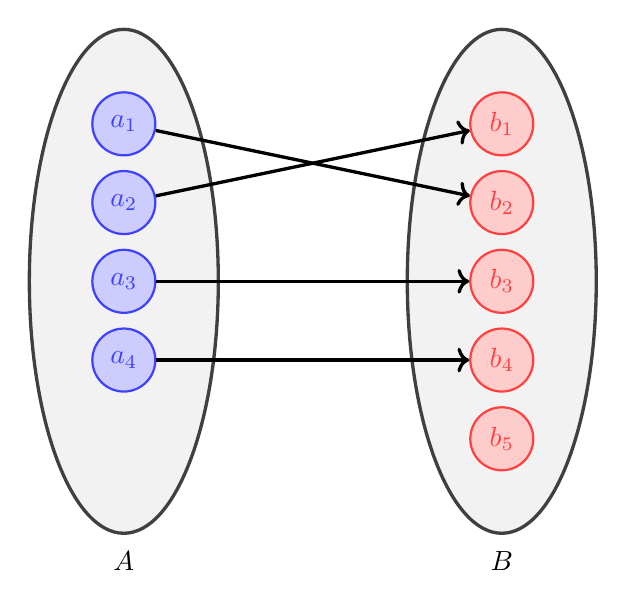
\begin{tikzpicture}[scale=0.8]
        \tikzstyle{blue-node}=[color=blue!75,fill=blue!20,thick,circle, draw, minimum width=0.8cm]
        \tikzstyle{red-node}=[color=red!75,fill=red!20,thick,circle, draw, minimum width=0.8cm]
        \tikzstyle{parent}=[color=black!75,fill=black!5,very thick]
        \tikzstyle{mapsto}=[->,very thick]
        % set A
        \draw [parent] (-2,0) ellipse (1.5cm and 4cm);       
        \node [blue-node] at (-2,2.5) (a1) {$a_1$};        
        \node [blue-node] at (-2,1.25) (a2) {$a_2$};
        \node [blue-node] at (-2,0) (a3) {$a_3$};
        \node [blue-node] at (-2,-1.25) (a4) {$a_4$} (-2,-4.75) node[anchor=south,color=black] {$A$};
        % set B
        \draw [parent] (4,0) ellipse (1.5cm and 4cm);
        \node [red-node] at (4,2.5) (b1) {$b_1$};
        \node [red-node] at (4,1.25) (b2) {$b_2$};
        \node [red-node] at (4,0)(b3) {$b_3$};
        \node [red-node] at (4,-1.25) (b4) {$b_4$};
        \node [red-node] at (4,-2.5) (b5) {$b_5$} (4,-4.75) node[anchor=south,color=black] {$B$};
        % mapsto
        \draw [mapsto] (a1) -- (b2);
        \draw [mapsto] (a2) -- (b1);
        \draw [mapsto] (a3) -- (b3);
        \draw [mapsto] (a4) -- (b4);
    \end{tikzpicture}
    \caption{Example of an injective function}
    \label{sketch-injective-function}
\end{figure}

\begin{exm}\label{exm-surjective-function}
    Let $f:\mathbb{R}\rightarrow\mathbb{R},f(x)=2x+3$. Is this function surjective?
    \begin{flushleft}
        \textbf{Answer}: For any $y=f(x)\in\mathbb{R}$ there exists an $x=\frac{y-3}{2}$
        such that
        \begin{align*}
            f(x) &= 2\left(\frac{y-3}{2}\right)+3 \\
                 &= y - 3 + 3 \\
                 &= y
        \end{align*}
        This proves that the function $f(x)=2x+3$ is surjective since $\text{Im}(f)=\mathbb{R}$. 
        With respect to \pref{figure}{sketch-surjective-function} this means that 
        every value from the codomain is taken on \textit{at least} once.
    \end{flushleft}
    \begin{rem}
        The strategy for determining whether a function is 
        surjective or not boils down to solving the original function definition
        for $x$ and plugging in this expression in $f(x)$. If you can show that 
        $f(x)=y$ then you are done, if not then the function is not surjective.
    \end{rem}
\end{exm}

\begin{figure}[ht!]
    \centering
    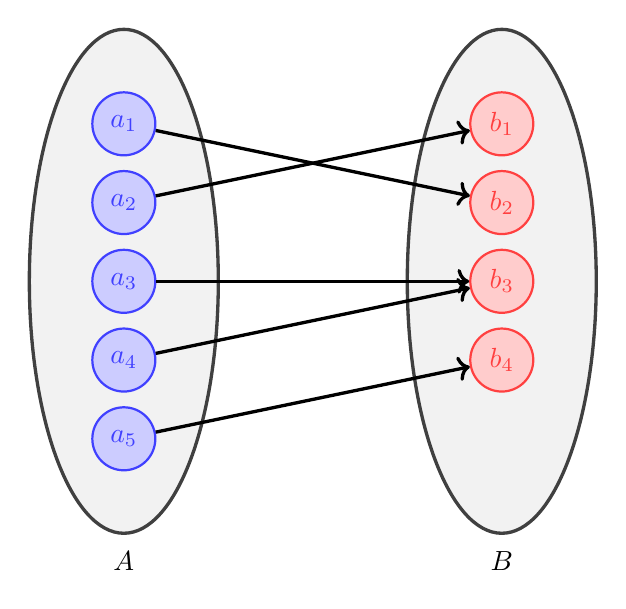
\begin{tikzpicture}[scale=0.8]
        \tikzstyle{blue-node}=[color=blue!75,fill=blue!20,thick,circle, draw, minimum width=0.8cm]
        \tikzstyle{red-node}=[color=red!75,fill=red!20,thick,circle, draw, minimum width=0.8cm]
        \tikzstyle{parent}=[color=black!75,fill=black!5,very thick]
        \tikzstyle{mapsto}=[->,very thick]
        % set A
        \draw [parent] (-2,0) ellipse (1.5cm and 4cm);       
        \node [blue-node] at (-2,2.5) (a1) {$a_1$};        
        \node [blue-node] at (-2,1.25) (a2) {$a_2$};
        \node [blue-node] at (-2,0) (a3) {$a_3$};
        \node [blue-node] at (-2,-1.25) (a4) {$a_4$};
        \node [blue-node] at (-2,-2.5) (a5) {$a_5$} (-2,-4.75) node[anchor=south,color=black] {$A$};
        % set B
        \draw [parent] (4,0) ellipse (1.5cm and 4cm);
        \node [red-node] at (4,2.5) (b1) {$b_1$};
        \node [red-node] at (4,1.25) (b2) {$b_2$};
        \node [red-node] at (4,0)(b3) {$b_3$};
        \node [red-node] at (4,-1.25) (b4) {$b_4$} (4,-4.75) node[anchor=south,color=black] {$B$};
        % mapsto
        \draw [mapsto] (a1) -- (b2);
        \draw [mapsto] (a2) -- (b1);
        \draw [mapsto] (a3) -- (b3);
        \draw [mapsto] (a4) -- (b3);
        \draw [mapsto] (a5) -- (b4);
    \end{tikzpicture}
    \caption{Example of an surjective function}
    \label{sketch-surjective-function}
\end{figure}

\begin{exm}\label{exm-bijective-function}
    Let $f:\mathbb{R}\rightarrow\mathbb{R},f(x)=2x+3$. Is this function bijective?
    \begin{flushleft}
        \textbf{Answer}: From \pref{example}{exm-injective-function} and
        \pref{example}{exm-surjective-function} we can deduce that since the function
        is injective and surjective, that it is bijective as well. With respect 
        to \pref{figure}{sketch-bijective-function} this means that every value 
        from the codomain is taken on \textit{exactly} once.
    \end{flushleft}
\end{exm}

\begin{figure}[ht!]
    \centering
    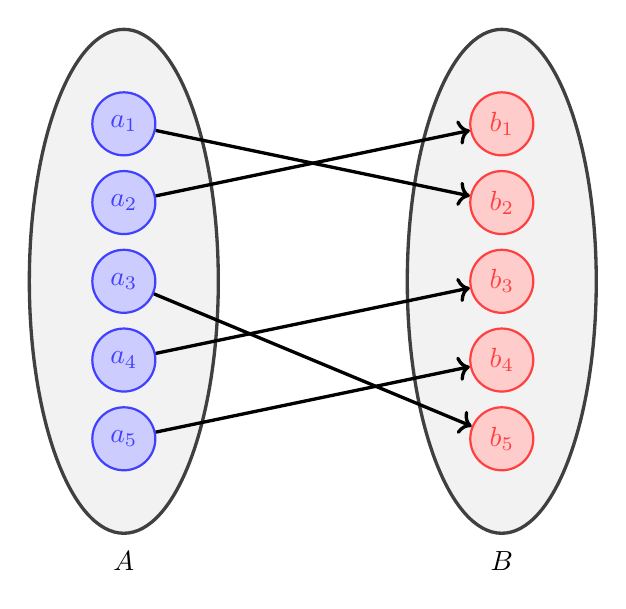
\begin{tikzpicture}[scale=0.8]
        \tikzstyle{blue-node}=[color=blue!75,fill=blue!20,thick,circle, draw, minimum width=0.8cm]
        \tikzstyle{red-node}=[color=red!75,fill=red!20,thick,circle, draw, minimum width=0.8cm]
        \tikzstyle{parent}=[color=black!75,fill=black!5,very thick]
        \tikzstyle{mapsto}=[->,very thick]
        % set A
        \draw [parent] (-2,0) ellipse (1.5cm and 4cm);       
        \node [blue-node] at (-2,2.5) (a1) {$a_1$};        
        \node [blue-node] at (-2,1.25) (a2) {$a_2$};
        \node [blue-node] at (-2,0) (a3) {$a_3$};
        \node [blue-node] at (-2,-1.25) (a4) {$a_4$};
        \node [blue-node] at (-2,-2.5) (a5) {$a_5$} (-2,-4.75) node[anchor=south,color=black] {$A$};
        % set B
        \draw [parent] (4,0) ellipse (1.5cm and 4cm);
        \node [red-node] at (4,2.5) (b1) {$b_1$};
        \node [red-node] at (4,1.25) (b2) {$b_2$};
        \node [red-node] at (4,0)(b3) {$b_3$};
        \node [red-node] at (4,-1.25) (b4) {$b_4$};
        \node [red-node] at (4,-2.5) (b5) {$b_5$} (4,-4.75) node[anchor=south,color=black] {$B$};
        % mapsto
        \draw [mapsto] (a1) -- (b2);
        \draw [mapsto] (a2) -- (b1);
        \draw [mapsto] (a3) -- (b5);
        \draw [mapsto] (a4) -- (b3);
        \draw [mapsto] (a5) -- (b4);
    \end{tikzpicture}
    \caption{Example of an bijective function}
    \label{sketch-bijective-function}
\end{figure}

\begin{exm}\label{exm-injective-surjective-bijective}
    Determine whether the following functions are injective, surjective or
    bijective\footnote{You may also consult \pref{figure}{sktech:exm-1:4} for
    additional help.}:
    \begin{enumerate}
        \item[1.)] $f(x):\mathbb{R}^+\rightarrow\mathbb{R}^+,x\mapsto x^2-1$
        \item[2.)] $g(x):\mathbb{R}^+\rightarrow\mathbb{R},x\mapsto x^2-1$
        \item[3.)] $h(x):\mathbb{R}\rightarrow\mathbb{R}^+,x\mapsto x^2-1$
        \item[4.)] $i(x):\mathbb{R}\rightarrow\mathbb{R},x\mapsto x^2-1$ 
    \end{enumerate}
    \begin{flushleft}
        \textbf{Answer:} TODO
    \end{flushleft}
\end{exm}

\begin{definition}\label{def-inverse-function}
    Let $f:\mathcal{D}\to\mathcal{C}$. We say that $f$ is invertible if there exists
    $f^{-1}:\mathcal{C}\to\mathcal{D}$ such that
    \begin{equation}
        \forall x\in\mathcal{D}:(f^{-1}\circ f)(x)=x 
        \land \forall y\in\mathcal{C}:(f \circ f^{-1})(y)=y
    \end{equation}
    If that's the case, we call $f^{-1}$ the inverse function of $f$.
\end{definition}

\begin{thm}\label{thm-inverse-function}
    A function $f$ is invertible, \textit{iff} it is bijective.
\end{thm}

\begin{rem}\label{rem-sqrt-function}
    In school we learnt that the function 
    \begin{equation}\label{eq-sqrt-function}
        f:\mathbb{R}^+\to\mathbb{R}^+,x\mapsto\sqrt{x}
    \end{equation}
    is the inverse function of
    \begin{equation}\label{eq-pow-function}
        f:\mathbb{R}\to\mathbb{R}^+,x\mapsto x^2
    \end{equation}
    Notice that the square root function in \pref{equation}{eq-sqrt-function} is 
    only defined for positive values on $\mathbb{R}$. This is because the principal
    square root is positive:
    \begin{equation}\label{eq-sqrt-abs-function}
        \sqrt{x^2}=\abs{x}
    \end{equation}
    You may have been taught in physics that the square root function can take on
    two values, \textit{i.e.} $\sqrt{x^2}=\pm x$, for example
    \begin{equation*}
        f(x=9)=\sqrt{9}\implies x=3 \lor x=-3
    \end{equation*}
    But \pref{theorem}{thm-inverse-function} states that inverse functions are 
    bijective\footnote{To satisfy this old notion, the square root function would
    have to be strictly surjective, see also \pref{figure}{sketch-surjective-function}.}.
    \begin{figure}[h!]
        \centering
        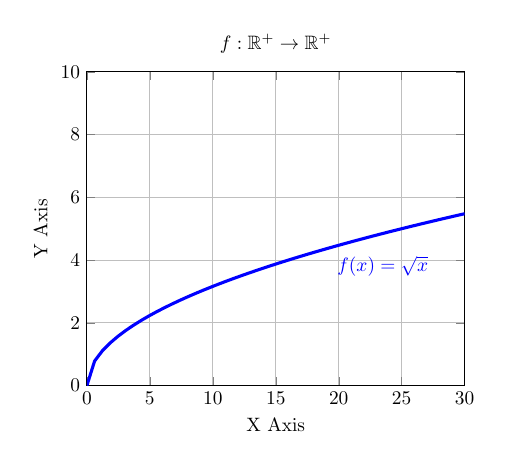
\begin{tikzpicture}[scale=0.7]
            \begin{axis}[
                xmax=30,
                xmin=0,
                ymax=10,
                ymin=0,
                samples=50,
                grid=major,
                xlabel={X Axis},
                ylabel={Y Axis},
                title={$f:\mathbb{R}^+\to\mathbb{R}^+$}
            ]
            \addplot[blue, ultra thick,domain=0:30]{sqrt(x)} node[anchor=north west,pos=0.65] {$f(x)=\sqrt{x}$};
        \end{axis}
        \end{tikzpicture}
        \caption{The square root function only operates with positive numbers}
        \label{sketch:rem-sqrt-function}
    \end{figure}
    So, while it is sometimes convenient to follow the convention in \pref{equation}{eq-sqrt-abs-function},
    strictly speaking the square root function only ever takes on positive values
    (\textit{cf.} \pref{figure}{sketch:rem-sqrt-function}).
\end{rem}

\begin{definition}\label{def-floor-function}
    The floor function is defined by
    \begin{equation}
        \ffloor(x)=\floor{x}\defines\max\left\{m\in\mathbb{Z}\setbuild m\leq x\right\}
    \end{equation}
\end{definition}

\begin{definition}\label{def-ceiling-function}
    The ceiling function is defined by
    \begin{equation}
        \fceil(x)=\ceil{x}\defines\min\left\{n\in\mathbb{Z}\setbuild n\geq x\right\}
    \end{equation}
\end{definition}

\begin{definition}\label{def-dirichlet-function}
    The Dirichlet function is defined by
    \begin{equation}
        D(x)=\begin{cases}
            1\text{ if }x\in\mathbb{Q}\\
            0\text{ else }
        \end{cases}
    \end{equation}
\end{definition}

\begin{definition}\label{def-absolute-value-function}
    The absolute value function is defined by
    \begin{equation}
        \forall x\in\mathbb{R}: \abs{x}\defines\max\{x,-x\}=\begin{cases}
            x\text{ if } x \geq 0 \\
            -x \text{ else }
        \end{cases}
    \end{equation}
\end{definition}

\begin{thm}\label{thm-absolute-value-properties}
    Below are listed some of the properties related to the absolute value; for
    any $x\in\mathbb{R}$ the following holds:
    \begin{enumerate}
        \item $\abs{x} \geq 0$
        \item $\abs{x} \geq \pm x$
        \item $\abs{x} = \abs{-x}$
        \item $\abs{x} = 0 \iff x = 0$
        \item $\abs{xy} = \abs{x}\abs{y}$
        \item $\abs{x} + \abs{y} \geq \abs{x+y}$
        \item $\abs{x-y} \geq \abs[\big]{\abs{x}-\abs{y}}$
        \item $\abs{x} < M \iff -M < x < M$
    \end{enumerate}
\end{thm}

\begin{proof}
    Of theorem (\ref{thm-absolute-value-properties}).
    \begin{flushleft}
        In this proof we will only show property 6 of this theorem which is also
        known as the triangle inequality. From property 2 it follows that the sum 
        of $\abs{x}\geq x$ and $\abs{y}\geq y$ equals
        \begin{equation}\label{tmp-absolute-value-properties:1}
            \abs{x} + \abs{y} \geq x + y
        \end{equation}
        Likewise, from $\abs{x}\geq -x$ and $\abs{y}\geq -y$ it follows that
        \begin{equation}\label{tmp-absolute-value-properties:2}
            \abs{x} + \abs{y} \geq -(x+y)
        \end{equation}
        Thus, by definition (\ref{def-absolute-value-function}) and equation
        (\ref{tmp-absolute-value-properties:1}) and (\ref{tmp-absolute-value-properties:2})
        we can conclude that
        \begin{equation*}
            \abs{x} + \abs{y} \geq \abs{x+y}
        \end{equation*}
    \end{flushleft}
\end{proof}

\begin{rem}
    A geometric interpretation of the absolute value function $\abs{x}$ is the 
    distance from $x$ to $0$. Similarly, the absolute value of the difference 
    $\abs{x-y}$ can be interpreted as the distance between $x$ and $y$. See also
    \hyperref[subsec-metric-spaces]{the subsection for metric spaces} for more 
    more information on distances.
\end{rem}

\subsection{Limit Prerequisites}\label{subsec-limit-prerequisites}

\begin{definition}\label{def-interval-notation}
    As opposed to closed intervals, open and half-open intervals contain infinitely
    many elements. The $\infty$ symbol always needs to be paired with a parenthesis
    rather than a bracket because it is technically incorrect to think of infinity
    as a number. So far, we haven't agreed on a formal definition for the concept
    of infinity, but it will become important later when we discuss limits in more
    detail.
    \begin{enumerate}
        \item $(a,b)\defines\left\{x\setbuild a < x < b\right\}       \quad \text{(Open interval)}$
        \item $(a,b]\defines\left\{x\setbuild a < x \leq b\right\}    \quad \text{(Half-open interval)}$
        \item $[a,b)\defines\left\{x\setbuild a \leq x < b\right\}    \quad \text{(Half-closed interval)}$
        \item $[a,b]\defines\left\{x\setbuild a \leq x \leq b\right\} \quad \text{(Closed interval)}$
    \end{enumerate}
\end{definition}

\begin{definition}\label{def-epsilon-neighborhood}
    Let $a\in\mathbb{R}$ and $\varepsilon > 0$. Then the open interval 
    $(a-\varepsilon,a+\varepsilon)$ is called the epsilon neighborhood of $a$
    and is denoted by
    \begin{equation}
        \mathcal{U}_\varepsilon(a)\defines
        \left\{x \setbuild x\in\mathbb{R},\abs{x-a}<\varepsilon \right\}=
        (a-\varepsilon,a+\varepsilon)
    \end{equation}
\end{definition}

\begin{rem}\label{rem-epsilon-neighborhood}
    In reference to property 8 of theorem (\ref{thm-absolute-value-properties})
    we can note that
    \begin{equation}
        x\in(a-\varepsilon,a+\varepsilon) \iff \abs{x-a} < \varepsilon
    \end{equation}
\end{rem}

\begin{definition}\label{def-epsilon-punctured-neighborhood}
    Let $a\in\mathbb{R}$. For $\varepsilon>0$ we define the punctured epsilon 
    neighborhood of $a$, denoted by 
    \begin{equation}
        \mathcal{U}_{\varepsilon}^{\bolddot}(a)\defines
        \left\{x \setbuild x\in\mathbb{R}, 0<\abs{x-a}<\varepsilon\right\}=
        (a-\varepsilon,a+\varepsilon)\setminus\{a\}
    \end{equation}
\end{definition}

\begin{definition}\label{def-limit-point}
    Let $M\subset\mathbb{R}$ and $a\in\mathbb{R}$. Then, $a$ is called a limit 
    point\footnote{Or cluster point} of $M$ \textit{iff}
    \begin{equation}
        \bigwedge_{\varepsilon>0}(M\cap\mathcal{U}_\varepsilon^{\bolddot}\neq\emptyset)
    \end{equation}
\end{definition}

\begin{definition}\label{def-isolated-point}
    In contrast to definition (\ref{def-limit-point}), we call $a$ an isolated point
    of $M$ \textit{iff}
    \begin{equation}
        \neg\bigwedge_{\varepsilon>0}(M\cap\mathcal{U}_\varepsilon^{\bolddot}\neq\emptyset)
        \iff
        \bigvee_{\varepsilon>0}(M\cap\mathcal{U}_\varepsilon^{\bolddot}=\emptyset)
    \end{equation}
    \textit{i.e.} $a\in M\subset\mathbb{R}$ and $a$ is not a limit point.
\end{definition}

\begin{rem}
    If $a$ is an isolated point of $M$, then \cite[p.67]{wuest2009}
    \begin{align*}
        a\in M:\mathcal{U}_\varepsilon(a)
        &=(\{a\}\cup\mathcal{U}_\varepsilon^{\bolddot})\cap M \\
        &=(\{a\}\cap M)\cup(\mathcal{U}_\varepsilon^{\bolddot}\cap M) \\
        &=\{a\}
    \end{align*}
    Therefore, in the neighborhood of $a$ are no other elements of the set $M$.
\end{rem}

\begin{exm}\label{exm-limit-points}
    Find the set of all limit points for
    \begin{enumerate}
        \item $A\defines\displaystyle\bigcup_{n\in\mathbb{N}}\left(\frac{1}{n},2-\frac{1}{n}\right)$
        \item $B\defines\left\{x\in\mathbb{R}\setbuild x=n+\frac{1}{m}\quad\text{($n,m$ appropriate)}\right\}$
    \end{enumerate}
    \begin{flushleft}
        \textbf{\nth{1} Answer:} TODO
    \end{flushleft}
    \begin{flushleft}
        \textbf{\nth{2} Answer:} TODO
    \end{flushleft}
\end{exm}

\begin{definition}\label{def-bounded-sets}
    Let $A \subseteq\mathbb{R}$ be a set.
    \begin{enumerate}
        \item Then $A$ is called bounded from above if there exists $M\in\mathbb{R}$ 
        such that $x\leq M$ for any $x\in A$.
        \item Similarly, $A$ is bounded from below if there exists $m\in\mathbb{R}$ 
        such that $x\geq M$ for any $x\in A$.
        \item Finally, $A$ is called bounded if it is bounded from above and below.
        \footnote{Notice that the boundary points in this definition
        lay no claim to uniqueness.}
    \end{enumerate}
\end{definition}

\begin{exm}\label{exm-bounded-sets:1}
    \hfill
    \begin{enumerate}
        \item Consider the set of natural numbers: $\mathbb{N}$ is not bounded from above, but 
        below, \textit{i.e.} $1$ is a lower bound of $\mathbb{N}$.
        \item Let $A=(-3,2]$. Then this set is bounded from above and below.
        \item Let $B=\left\{\frac{1}{n}\setbuild n\in\mathbb{N}\right\}$. Then this
        set is bounded from above by $1$, and bounded from below by $0$.
    \end{enumerate}
\end{exm}

\begin{definition}\label{def-supremum-infimum-sets}
    Let $A\subset\mathbb{R}$ be a set.
    \begin{enumerate}
        \item $S$ is called the supremum of $A$ if it is the smallest upper bound 
        of $A$, and is denoted by $S=\sup(A)$.
        \item $I$ is called the infimum of $A$ if it is the largest lower bound 
        of $A$, and is denoted by $I=\inf(A)$.
    \end{enumerate}
\end{definition}

\begin{exm}\label{exm-bounded-sets:2}
    Consider the sets from \pref{example}{exm-bounded-sets:1}. Then\footnote{Remark:
    $\mathbb{N}\defines\{1,2,3,\dots\}$}
    \begin{enumerate}
        \item $\inf(\mathbb{N})=1$
        \item $\inf(A)=-3$ and $\sup(A)=2$
        \item $\inf(B)=0$ and $\sup(B)=1$
    \end{enumerate}
\end{exm}

\begin{definition}\label{def-maximum-minimum}
    Let $A\subset\mathbb{R}$ be a set.
    \begin{enumerate}
        \item If $S=\sup(A)$, then $S\in A$ is also a maximum of $A$ and is denoted by $S=\max(A)$.
        \item If $I=\inf(A)$, then $I\in A$ is also a minimum of $A$ and is denoted by $I=\min(A)$.
    \end{enumerate}
\end{definition}

\begin{exm}\label{exm-bounded-sets:3}
    Expanding on the results from example (\ref{exm-bounded-sets:2}), we note that
    \begin{enumerate}
        \item $\min(\mathbb{N})=1$
        \item $\min(A)=\text{\gls{dne}}$ and $\max(A)=2$
        \item $\min(B)=\text{\gls{dne}}$ and $\max(B)=1$
    \end{enumerate}
\end{exm}

\begin{definition}\label{def-monotonicity}
    Let $x,y\in\mathbb{R}$. A function is called
    \begin{enumerate}
        \item monotonically increasing, if for all $x,y$ it follows that
        \begin{equation}\label{eq-monotonically-increasing}
            x<y \implies f(x)\leq f(y)
        \end{equation}
        \item strictly monotonically increasing, if for all $x,y$ follows that
        \begin{equation}\label{eq-strictly-monotonically-increasing}
            x<y \implies f(x)<f(y)
        \end{equation}
        \item monotonically decreasing, if for all $x,y$ follows that
        \begin{equation}\label{eq-monotonically-decreasing}
            x<y \implies f(x)\geq f(y)
        \end{equation}
        \item strictly monotonically decreasing, if for all $x,y$ follows that
        \begin{equation}\label{eq-strictly-monotonically-decreasing}
            x<y \implies f(x)>f(y)
        \end{equation}
    \end{enumerate}
\end{definition}

\begin{exm}
    Let $f(x)=\sin(x)$.
    \begin{enumerate}
        \item Then $f$ is strictly increasing on $[-\tfrac{\pi}{2},\tfrac{\pi}{2}]$.
        \item Then $f$ is strictly decreasing on $[\tfrac{\pi}{2},\tfrac{3\pi}{2}]$.
    \end{enumerate}
\end{exm}

\begin{definition}\label{def-even-function}
    Let $f$ be a function. Then, $f$ is called an even function if
    \begin{equation}
        \forall x\in\domain{f}:f(x)=f(-x)
    \end{equation}
\end{definition}

\begin{exm}
    See the list below for some even functions:
    \begin{itemize}
        \item $x\mapsto\abs{x}$
        \item $x\mapsto x^2$
        \item $x\mapsto\cos(x)$
    \end{itemize}
\end{exm}

\begin{definition}\label{def-odd-function}
    Let $f$ be a function. Then, $f$ is called an odd function if
    \begin{equation}
        \forall x\in\domain{f}:f(x)=-f(-x)
    \end{equation}
\end{definition}

\begin{exm}
    See the list below for some odd functions:
    \begin{itemize}
        \item $x\mapsto x$
        \item $x\mapsto x^3$
        \item $x\mapsto\sin(x)$
    \end{itemize}
\end{exm}

\begin{definition}
    Let $f$ be a function. Then, $f$ is called a periodic function if
    \begin{equation}
        \forall x\in\domain{f}\,\exists T\in\mathbb{R}: f(x)=f(x+T)
    \end{equation}
\end{definition}

\begin{exm}
    See the list below for some periodic functions:
    \begin{itemize}
        \item $x\mapsto\sin(x)$
        \item $x\mapsto\cos(x)$
        \item $x\mapsto\tan(x)$
        \item \hyperref[def-dirichlet-function]{$x\mapsto D(x)$}
    \end{itemize}
\end{exm}

\begin{definition}\label{def-bounded-function}
    Let $f$ be a function. Then, $f$ is called\footnote{This definition extends 
    the notion of boundaries as defined in \pref{definition}{def-bounded-sets} to 
    functions.}
    \begin{enumerate}
        \item bounded from above if
        \begin{equation}
            \forall x\in\domain{f}\,\exists M\in\mathbb{R}:f(x)\leq M
        \end{equation}
        \item bounded from below if 
        \begin{equation}
            \forall x\in\domain{f}\,\exists m\in\mathbb{R}:f(x)\geq m
        \end{equation}
        \item bounded if $f$ is bounded from above and below.
    \end{enumerate}
\end{definition}

\begin{exm}
    The function $f:\mathcal{D}\to\mathbb{R}$ with
    \begin{itemize}
        \item $\domain{f}=\mathbb{R}^-:f(x)=x$ is bounded from above but not below
        \item $\domain{f}=\mathbb{R}:f(x)=x^2$ is bounded from below, but not above
        \item $\domain{f}=\mathbb{R}^+:f(x)=\sqrt{x}$ is bounded from below, but not above
        \item $\domain{f}=\mathbb{R}:f(x)=\sin(x)$ is bounded from above and below
        \item $\domain{f}=\mathbb{R}:f(x)=\ffloor(x)$ is neither bounded from above nor below
    \end{itemize}
\end{exm}

\begin{rem}\label{rem-bounded-function}
    A function $f$ is bounded \textit{iff}
    \begin{equation}
        \forall x\in\domain{f}\,\exists B\in\mathbb{R}:\abs{f(x)}\leq B
    \end{equation}
    since $\abs{f(x)}\leq B\iff -B\leq f(x) \leq B$ by the \nth{8} property from
    \pref{theorem}{thm-absolute-value-properties}.
\end{rem}

\begin{definition}\label{def-supremum-infimum-functions}
    Let $f$ be a function. Then we define
    \begin{enumerate}
        \item the supremum of a function by
        \begin{equation}
            \sup_{x\in\mathcal{D}}(f)\defines\sup\left\{f(x)\setbuild x\in\mathcal{D}\right\}
        \end{equation}
        \item the infimum of a function by
        \begin{equation}
            \inf_{x\in\mathcal{D}}(f)\defines\inf\left\{f(x)\setbuild x\in\mathcal{D}\right\}
        \end{equation}
    \end{enumerate}
\end{definition}

\begin{exm}
    Let $f(x)=\arctan(x)$. Then,
    \begin{itemize}
        \item the supremum of this function is
        \begin{equation}
            \sup(f)=\frac{\pi}{2}
        \end{equation}
        \item the infimum of this function is
        \begin{equation}
            \inf(f)=-\frac{\pi}{2}
        \end{equation}
    \end{itemize}
\end{exm}

\begin{definition}\label{def-function-operations}
    Let $f$ and $g$ be two functions. Then we define
    \begin{enumerate}
        \item the addition between two functions by
        \begin{equation}
            (f \pm g)(x) \defines f(x) \pm g(x)
        \end{equation}
        \item the multiplication between two functions by
        \begin{equation}
            (f \cdot g)(x) \defines f(x) \cdot g(x)
        \end{equation}
        \item the division between two functions by\footnote{For $g(x)\neq0$}
        \begin{equation}
            \left(\frac{f}{g}\right)(x) \defines \frac{f(x)}{g(x)} 
        \end{equation}
        \item the composition between two functions by
        \begin{equation}
            (f \circ g)(x) \defines f(g(x))
        \end{equation}
    \end{enumerate}
\end{definition}

\begin{exm}
    Let $f:\mathbb{R}\to[-1,1],x\mapsto\sin(x)$ and $g:\mathbb{R}\setminus\{0\}\to\mathbb{R},x\mapsto\tfrac{1}{x}$.
    Then the two compositions for these functions are given by
    \begin{align*}
        &(f \circ g):\mathbb{R}\setminus\{0\}\to[-1,1],x\mapsto\sin\left(\frac{1}{x}\right)\\
        &(g \circ f):\mathbb{R}\setminus\left\{\pi k\setbuild k\in\mathbb{Z}\right\}\to\mathbb{R},x\mapsto\frac{1}{\sin(x)}
    \end{align*}
\end{exm}

\begin{rem}\label{rem-monotone-implies-injective}
    If $f$ is strictly monotone, then $f$ is injective.
\end{rem}

\begin{rem}\label{rem-elementary-functions}
    It is advised to remember the following elementary functions by heart:
    \begin{itemize}
        \item Polynomial functions\footnote{$a_0$ is the so-called \enquote{free coefficient}}: $p(x)=\sum_{i=0}^na_ix^i$
        \item Rational functions: $f(x)=\tfrac{p(x)}{q(x)}$ where $p(x)$ and $q(x)$ are well-defined polynomial functions
        \item Exponential functions: $f(x)=a^x$ for $a>0$ and $a\neq 1$
        \item Trigonometric functions: for example, $f(x)=\sin(x)$
        \item Inverse trigonometric functions: for example, $f^{-1}(x)=\arcsin(x)$
        \item Inverse functions of polynomials, for example $f^{-1}(x)=\sqrt{x}$
        \item Inverse functions of rationals
        \item Inverse functions of exponentials: for example, $f^{-1}(x)=\log_a(x)$
    \end{itemize}
\end{rem}

\begin{definition}\label{def-elementary-functions}
    An elementary function is any function obtained from the list in \pref{remark}{rem-elementary-functions},
    including their combinations using the operations defined in \pref{definition}{def-function-operations}.
    \footnote{Note that this is not a standard definition.}
\end{definition}

\subsection{Limits}\label{subsec-limits}

\begin{definition}\label{def-epsilon-delta-definition-limit}
	Let $f(x)$ be a function with $a,b\in\mathbb{R}$ with $a$ as a limit point of $\domain{f}$.
	Then the the function $f$ has the limit $b$ as $x$ approaches $a$, \textit{i.e.}
	\begin{equation}
		\bigwedge_{\varepsilon>0}\bigvee_{\delta>0}\bigwedge_{x\in\domain{f}}
		\left(0<\abs{x-a}<\delta\implies\abs{f(x)-b}<\varepsilon\right)
	\end{equation}
	The limit of this function is denoted by
	\begin{equation}
		\lim_{x\to a}f(x)=b,
	\end{equation}
\end{definition}

\begin{rem}
	The equation $\displaystyle\lim_{x\to a}f(x)=b$ is equivalent to the following
	expressions:
	\begin{enumerate}
		\item For $f$ there exists a limit (point) at $a$.
		\item This limit of $f$ is equal to $b$.
	\end{enumerate}
	In other words, $f$ has a limit at $a$ if
	\begin{equation*}
		\bigvee_{b\in\mathbb{R}}\bigwedge_{\varepsilon>0}\bigvee_{\delta>0}\bigwedge_{x\in\domain{f}}
		\left(0<\abs{x-a}<\delta \implies \abs{f(x)-b}<\varepsilon\right)
	\end{equation*}
\end{rem}

\begin{exm}\label{exm-epsilon-delta-definition-limit:1}
	Show that
	\begin{equation*}
		\lim_{x\to3}\frac{x-1}{2}=1
	\end{equation*}
	by using the epsilon-delta definition for limits.
	\begin{flushleft}
		\textbf{Answer}: Let $\varepsilon>0$ and $b\in\mathbb{R}$. Take
		$\delta\defines2\varepsilon$; Then $\abs{x-3}<\delta$, which implies
		\begin{align*}
			\abs{f(x)-b} & =\abs[\Bigg]{\frac{x-1}{2}-1} \\
			             & =\frac{\abs{x-3}}{2}          \\
			             & <\frac{\delta}{2}             \\
			             & =\varepsilon
		\end{align*}
	\end{flushleft}
\end{exm}

\begin{exm}\label{exm-epsilon-delta-definition-limit:2}
	Show that for some $a\in\mathbb{R}$,
	\begin{equation*}
		\lim_{x\to a}\sin(x)=\sin(a)
	\end{equation*}
	by using the epsilon-delta definition for limits.
	\begin{flushleft}
		\textbf{Answer}: Let $\varepsilon>0$ and $b\in\mathbb{R}$. Take
		$\varepsilon\defines\delta$ such that $\abs{x-a}<\delta$. Further, recall that
		\begin{align*}
			 & \text{(A)}:\forall\alpha\in\mathbb{R}:\abs{\cos(\alpha)}\leq1            \\
			 & \text{(B)}:\forall\alpha\in\mathbb{R}:\abs{\sin(\alpha)}\leq\abs{\alpha}
		\end{align*}
		\begin{align*}
			\abs{f(x)-b} & =\abs{\sin(x)-\sin(a)}                                                                                                    \\
			             & =\abs[\Bigg]{2\sin\left(\frac{x-a}{2}\right)\cos\left(\frac{x+a}{2}\right)}                                               \\
			             & =2\cdot\abs[\Bigg]{\sin\left(\frac{x-a}{2}\right)}\abs[\Bigg]{\cos\left(\frac{x+a}{2}\right)}                             \\
			             & \leq 2\cdot\frac{\abs{x-a}}{2}                                                                &  & \text{note (A) \& (B)} \\
			             & =\varepsilon
		\end{align*}
	\end{flushleft}
\end{exm}

\begin{exm}\label{exm-epsilon-delta-definition-limit:3}
	Show \cite[p.69]{wuest2009} that the function $f(x)=\tfrac{x^2-3x+2}{x(x-1)}$
	with $x\in\mathbb{R}\setminus\{0,1\}$ has the limit $b=-1$ as $x\to1$.
	\begin{flushleft}
		\textbf{Answer}: Let $\varepsilon>0$.
		\begin{align}
			\abs{f(x)-(-1)} & =\abs[\Bigg]{\frac{x^2-3x+2}{x(x-1)}+1}\nonumber                             \\
			                & =\abs[\Bigg]{\frac{(x-2)(x-1)}{x(x-1)}+1}\nonumber                           \\
			                & =\abs[\Bigg]{\frac{x-2}{x}+1}\nonumber                                       \\
			                & =\abs[\Bigg]{\frac{2x-2}{x}}\nonumber                                        \\
			                & =\frac{2}{\abs{x}}\cdot\abs{x-1}\label{eq3-epsilon-delta-definition-limit:1}
		\end{align}
		Since we aim for the neighborhood of $x=1$ we can impose the following
		restriction on this inequality:
		\begin{equation}\label{eq3-epsilon-delta-definition-limit:2}
			0<\abs{x-1}<\frac{1}{2}
		\end{equation}
		This in turn implies
		\begin{align}
			\abs{x} & =\abs{x-1+1}\nonumber                                                                                                               \\
			        & \geq1-\abs{x-1}\nonumber                                                                                                            \\
			        & >1-\frac{1}{2}                                           &  & \text{\pref{equation}{eq3-epsilon-delta-definition-limit:2}}\nonumber \\
			        & =\frac{1}{2}\label{eq3-epsilon-delta-definition-limit:3}
		\end{align}
		Hence,
		\begin{align}
			\abs{f(x)-b} & =\frac{2}{\abs{x}}\cdot\abs{x-1}                             &  & \text{\pref{equation}{eq3-epsilon-delta-definition-limit:1}}\nonumber \\
			             & <\frac{2}{\tfrac{1}{2}}\cdot\abs{x-1}                        &  & \text{\pref{equation}{eq3-epsilon-delta-definition-limit:3}}\nonumber \\
			             & =4\cdot\abs{x-1}\label{eq3-epsilon-delta-definition-limit:4}
		\end{align}
	\end{flushleft}
	Let $q(\varepsilon)\defines\min\left\{\tfrac{\varepsilon}{4},\tfrac{1}{2}\right\}$.
	Then for all $\varepsilon>0$ there exists a $\delta\defines q(\varepsilon)$ such that
	for $x\in\domain{f}$ it follows that
	\begin{align*}
		0<\abs{x-1}<\delta \implies \abs{f(x)-(-1)} & <4\cdot\abs{x-1}             &  & \text{\pref{equation}{eq3-epsilon-delta-definition-limit:4}} \\
		                                            & <4\cdot\frac{\varepsilon}{4}                                                                   \\
		                                            & =\varepsilon
	\end{align*}
\end{exm}

\begin{exm}\label{exm-epsilon-delta-definition-limit:4}
	Show that the function $f(x)=\tfrac{x^2-4x+3}{2x-6}$ with $x\in\mathbb{R}\setminus\{3\}$
	has the limit $b=1$ as $x\to3$.
	\begin{flushleft}
		\textbf{Answer}: Let $\varepsilon>0$. Define $\delta\defines2\varepsilon$,
		such that $\abs{x-3}<\delta$, wherefore
		\begin{align*}
			\abs{f(x)-b} & =\abs[\Bigg]{\frac{x^2-4x+3}{2x-6}-1}     \\
			             & =\abs[\Bigg]{\frac{(x-1)(x-3)}{2(x-3)}-1} \\
			             & =\abs[\Bigg]{\frac{1}{2}(x-1)-1}          \\
			             & =\abs[\Bigg]{\frac{1}{2}x-\frac{3}{2}}    \\
			             & =\frac{1}{2}\abs{x-3}                     \\
			             & <\frac{1}{2}\cdot2\varepsilon             \\
			             & =\varepsilon
		\end{align*}
	\end{flushleft}
\end{exm}

\begin{exm}\label{exm-epsilon-delta-definition-limit:5}
	Show that for $a>0$ ($a\in\mathbb{R}$),
	\begin{equation*}
		\sqrt{x}\tolim{x}{a}\sqrt{a}
	\end{equation*}
	\begin{flushleft}
		\textbf{Answer}: Let $\varepsilon>0$. When we define $\delta\defines\min\left\{a,\varepsilon\sqrt{a}\right\}$,
		then $\abs{x-a}<\delta$ implies that
		\begin{align*}
			\abs{f(x)-b} & =\abs[\big]{\sqrt{x}-\sqrt{a}}                                                         \\
			             & =\frac{\abs[\big]{\sqrt{x}-\sqrt{a}}\left(\sqrt{x}+\sqrt{a}\right)}{\sqrt{x}+\sqrt{a}} \\
			             & =\frac{\abs{x-a}}{\sqrt{x}+\sqrt{a}}                                                   \\
			             & <\frac{\abs{x-a}}{\sqrt{a}}                                                            \\
			             & <\frac{\varepsilon\sqrt{a}}{\sqrt{a}}                                                  \\
			             & =\varepsilon
		\end{align*}
		Therefore,
		\begin{equation*}
			\lim_{x\to a}\sqrt{x}=\sqrt{a}
		\end{equation*}
	\end{flushleft}
\end{exm}

\begin{rem}\label{rem-undefined-limits}
	Examples of functions where \pref{definition}{def-epsilon-delta-definition-limit} breaks:
	\begin{enumerate}
		\item For any $a\in\mathbb{Z}$, the limit of $f(x)=\floor{x}$ does not exists.
		\item The limit $\displaystyle\lim_{x\to0}\tfrac{1}{x}$ does not exists.
		\item The limit $\displaystyle\lim_{x\to0}\tfrac{1}{x^2}$ does not exists.
		\item The limit $\displaystyle\lim_{x\to0}\sin\left(\tfrac{1}{x}\right)$ does not exists.
	\end{enumerate}
\end{rem}

\begin{thm}\label{thm-limit-arithmetic}
	Let $\displaystyle\lim_{x \to a}f(x) = b_1$ and $\displaystyle\lim_{x \to a}g(x) = b_2$
	be two well-defined limits. Then the following statements hold:
	\begin{enumerate}
		\item $c \cdot f(x) \tolim{x}{a} c \cdot b_1 \quad (c\in\mathbb{R})$
		\item $f(x) + g(x) \tolim{x}{a} b_1 + b_2$
		\item $f(x) \cdot g(c) \tolim{x}{a} b_1 \cdot b_2$
		\item $\tfrac{f(x)}{g(x)} \tolim{x}{a} \tfrac{b_1}{b_2} \quad (b_2 \neq 0)$
	\end{enumerate}
\end{thm}


\begin{proof}
	Of \pref{theorem}{thm-limit-arithmetic}.
	\begin{flushleft}
		\textbf{\nth{2} Property}. From \pref{definition}{def-epsilon-delta-definition-limit}
		we can note that
		\begin{align*}
			 & \forall\varepsilon>0\;\exists\delta_1>0:\,\abs{x-a}<\delta_1\implies\abs{f(x)-b_1}<\frac{\varepsilon}{2} \\
			 & \forall\varepsilon>0\;\exists\delta_2>0:\,\abs{x-a}<\delta_2\implies\abs{g(x)-b_2}<\frac{\varepsilon}{2}
		\end{align*}
		Define $\delta\defines\min\{\delta_1,\delta_2\}$ Then, if $\abs{x-a}<\delta$,
		it follows from the triangle inequality that
		\begin{align*}
			\abs{f(x)+g(x)-(b_1+b_2)} & =\abs{(f(x)-b_1)+(g(x)-b_2)}                 \\
			                          & \leq\abs{f(x)-b_1}+\abs{g(x)-b_2}            \\
			                          & <\frac{\varepsilon}{2}+\frac{\varepsilon}{2} \\
			                          & =\varepsilon
		\end{align*}
	\end{flushleft}
\end{proof}

\begin{exm}
	Find the limit of
	\begin{equation*}
		\lim_{x \to 0}\left(\arctan\left(2\sqrt{\frac{\cos(x)}{3x+4}}\right)\right)=\frac{\pi}{4}
	\end{equation*}
	\begin{flushleft}
		\textbf{Answer}: TODO
	\end{flushleft}
\end{exm}

\begin{thm}\label{thm-absolute-value-of-limit:1}
	If $f(x) \tolim{x}{a} 0$, then this is equivalent to
	$\abs{f(x)} \tolim{x}{a} 0$.
\end{thm}

\begin{thm}\label{thm-absolute-value-of-limit:2}
	Let $b\in\mathbb{R}$. If $f(x) \tolim{x}{a} b$, then
	this implies $\abs{f(x)} \tolim{x}{a} \abs{b}$.
\end{thm}

\begin{rem}
	Note that the opposite direction of \pref{theorem}{thm-absolute-value-of-limit:2}
	is in general not true. A counter example for this would be the
	\hyperref[def-dirichlet-function]{Dirichlet function}.
\end{rem}

\begin{proof}
	Of \pref{theorem}{thm-absolute-value-of-limit:2}.
	\begin{flushleft}
		Let $\varepsilon>0$. Then $\abs{x-a}<\delta$ implies that
		\begin{align*}
			\abs[\big]{\abs{f(x) - \abs{b}}} & \leq \abs{f(x) - b} \\
			                                 & <\varepsilon
		\end{align*}
		by using the reverse triangle inequality for absolute values.
	\end{flushleft}
\end{proof}

\begin{thm}\label{thm-limit-monotonicity}
	Let $f(x) \geq g(x)$ for any $x\in\mathcal{U}_{\varepsilon}^{\bolddot}(a)$.
	If the limit of $f(x)$ and $g(x)$ exist, then
	\begin{equation*}
		\lim_{x \to a}f(x) \geq \lim_{x \to a}g(x)
	\end{equation*}
\end{thm}

\begin{rem}
	As for \pref{theorem}{thm-limit-monotonicity}, if $f(x) \geq 0$,
	then
	\begin{equation*}
		\lim_{x \to a}f(x) \geq 0
	\end{equation*}
\end{rem}

\begin{rem}
	\pref{Theorem}{thm-limit-monotonicity} does not hold if we replace the greater
	than or equal to inequality with a strictly greater than inequality.
\end{rem}

\begin{thm}\label{thm-unique-limit}
	If the limit of $\displaystyle\lim_{x\to a}f(x)=b\in\mathbb{R}$ exists, then $b$ is unique.
\end{thm}

\begin{proof}
	Of \pref{theorem}{thm-unique-limit}.
	\begin{flushleft}
		Assume \gls{wlog} that $b<c$ are both limits of this function. Define
		$\varepsilon\defines\tfrac{c-b}{3}>0$. Then by
		\pref{definition}{def-epsilon-delta-definition-limit} we have that
		\begin{equation}\label{eq-unique-limit:1}
			\exists\delta_1\text{ s.t. }a-\delta_1<x<a+\delta_1 \implies b-\varepsilon<f(x)<b+\varepsilon
		\end{equation}
		Likewise we know that
		\begin{equation}\label{eq-unique-limit:2}
			\exists\delta_2\text{ s.t. }a-\delta_1<x<a+\delta_1 \implies c-\varepsilon<f(x)<c+\varepsilon
		\end{equation}
	\end{flushleft}
	Therefore by \pref{equation}{eq-unique-limit:1} and \pref{equation}{eq-unique-limit:2},
	it follows that
	\begin{equation*}
		\left(f(x)<b+\varepsilon<c+\varepsilon\right)\land\left(c+\varepsilon<f(x)\right)
	\end{equation*}
	which is a contradiction.
\end{proof}

\begin{thm}\label{def-limit-is-bounded}
	If the limit of $\displaystyle\lim_{x\to a}f(x)=b\in\mathbb{R}$ exists, then
	$f$ is bounded in a neighborhood of $a$.
\end{thm}

\begin{thm}\label{thm-sandwich-theorem}
	Suppose that for any $x$ in a neighborhood of $a$
	\begin{equation*}
		h(x) \leq f(x) \leq g(x)
	\end{equation*}
	Further assume that
	\begin{equation*}
		\lim_{x \to a}h(x) = b = \lim_{x \to a}g(x)
	\end{equation*}
	Then it follows that
	\begin{equation*}
		\lim_{x \to a}f(x) = b
	\end{equation*}
\end{thm}

\begin{proof}
	Of \pref{theorem}{thm-sandwich-theorem}.
	\begin{flushleft}
		Let $\varepsilon>0$. Take $\delta\defines\min\{\delta_1,\delta_2\}$ where
		\begin{align*}
			 & 0 < \abs{x - a} < \delta_1 \implies \abs{g(x) - b} < \varepsilon \iff b - \varepsilon < g(x) < b + \varepsilon, \\
			 & 0 < \abs{x - a} < \delta_2 \implies \abs{h(x) - b} < \varepsilon \iff b - \varepsilon < h(x) < b + \varepsilon
		\end{align*}
		Therefore, if $0 < \abs{x - a} < \delta$,
		\begin{equation*}
			b - \varepsilon < h(x) \leq f(x) \leq g(x) < b + \varepsilon
		\end{equation*}
		which is equivalent to
		\begin{equation*}
			\abs{f(x) - b} < \varepsilon \iff \lim_{x \to a}f(x) = b
		\end{equation*}
	\end{flushleft}
\end{proof}

\begin{thm}\label{thm-product-of-bounded-zero-limit}
	If $\displaystyle\lim_{x \to a}f(x) = 0$ and $g(x)$ is bounded in a neighborhood
	of $a$, then
	\begin{equation*}
		\lim_{x \to a} \left(f(x)\cdot g(x)\right) = 0
	\end{equation*}
\end{thm}

\begin{proof}
	Of \pref{theorem}{thm-product-of-bounded-zero-limit}.
	\begin{flushleft}
		Since $g(x)$ is bounded, we can write $\abs{g(x)} \leq M$. So,
		\begin{align*}
			 & -M \leq \abs{g(x)} \leq M                                                                                                                                                                   \\
			\implies
			 & -M\cdot\abs{f(x)} \leq \abs{f(x)}\cdot\abs{g(x)} \leq M\cdot \abs{f(x)}                                                                                                                     \\
			\implies
			 & -M\cdot \lim_{x \to a}\abs{f(x)} \leq  \lim_{x \to a}\left(\abs{f(x)}\cdot\abs{g(x)}\right) \leq M \cdot \lim_{x \to a}\abs{f(x)}                                                           \\
			\implies
			 & -M \cdot 0 \leq \abs{f(x)}\cdot\abs{g(x)} \leq M \cdot 0                                                                          &  & \text{\pref{theorem}{thm-absolute-value-of-limit:1}} \\
			\implies
			 & 0 \leq \abs{f(x)}\cdot\abs{g(x)} \leq 0                                                                                           &  & \text{\pref{theorem}{thm-limit-arithmetic}}          \\
			\implies
			 & \lim_{x \to a}\left(\abs{f(x)}\cdot\abs{g(x)}\right)=0                                                                            &  & \text{\pref{theorem}{thm-sandwich-theorem}}          \\
			\implies
			 & \lim_{x \to a}\left(f(x)\cdot g(x)\right)=0                                                                                       &  & \text{\pref{theorem}{thm-absolute-value-of-limit:1}} \\
		\end{align*}
	\end{flushleft}
\end{proof}

\begin{exm}
	The limit of the function
	\begin{equation*}
		f(x) = x\cdot\sin\left(\frac{1}{x}\right)
	\end{equation*}
	as $x \to 0$ is
	\begin{equation*}
		\lim_{x \to 0}\left(x\cdot\sin\left(\frac{1}{x}\right)\right)=0
	\end{equation*}
	by \pref{theorem}{thm-product-of-bounded-zero-limit} since $\sin\left(\tfrac{1}{x}\right)$
	is bounded\footnote{But in and of itself not defined at $x=0$} by $[-1,1]$
	and the left factor of this function is $x=0$ as $x \to 0$.
\end{exm}

\begin{definition}\label{def-one-sided-limits}
	We denote the one-sided limit of the function $f(x)$ approached from the right by
	\begin{equation*}
		\lim_{x \to a^+}f(x)=b
	\end{equation*}
	if and only if
	\begin{equation}
		\forall\varepsilon>0\;\exists\delta>0:x\in(a,a+\delta)\implies\abs{f(x)-b}<\varepsilon
	\end{equation}
	Conversely, the left-sided limit is denoted by
	\begin{equation*}
		\lim_{x \to a^-}f(x)=b
	\end{equation*}
	if and only if
	\begin{equation}
		\forall\varepsilon>0\;\exists\delta>0:x\in(a-\delta,a)\implies\abs{f(x)-b}<\varepsilon
	\end{equation}
\end{definition}

\begin{rem}\label{rem-one-sided-limits}
	With respect to \pref{definition}{def-one-sided-limits}, note that there exist
	several equivalent notations. So, the right-sided limit of $f(x)$ can be denoted
	by
	\begin{equation*}
		\lim_{x \to a^+}f(x)=b
		\iff
		\lim_{x \underset{x>a}{\to} a}f(x)=b
		\iff
		\lim_{x\searrow  a}f(x)=b
	\end{equation*}
	Similarly, at times the left-sided limits may be denoted by
	\begin{equation*}
		\lim_{x \to a^-}f(x)=b
		\iff
		\lim_{x \underset{x<a}{\to} a}f(x)=b
		\iff
		\lim_{x \nearrow a}f(x)=b
	\end{equation*}
\end{rem}

\begin{thm}\label{thm-limit-exists-one-sided-limits}
	The limit of $f(x) \to b$ exists as $x \to a$ if and only if the left-sided
	limit as well as the right-sided limit of $f$ exists with
	\begin{equation}
		\lim_{x \to a}f(x)=b \iff \lim_{x \to a^+}f(x)=b=\lim_{x \to a^-}f(x)
	\end{equation}
\end{thm}

\begin{proof}
	Of \pref{theorem}{thm-limit-exists-one-sided-limits}.
	\begin{flushleft}
		TODO
	\end{flushleft}
\end{proof}

\begin{exm}\label{exm-important-sin-over-x-limit}
	Show that\footnote{This is a very useful limit that we are going to encounter
		more often in the near future.}
	\begin{equation}\label{eq-important-sin-over-x-limit}
		\lim_{x \to 0}\frac{\sin(x)}{x}=1
	\end{equation}
	\begin{flushleft}
		\textbf{Answer}: From figure (??) we can derive two observations:
		\begin{equation*}
			\forall x\in\left(0,\frac{\pi}{2}\right)\implies \sin(x)<x
		\end{equation*}
		Notice also that
		\begin{equation*}
			x < \tan(x)
		\end{equation*}
		So, this implies
		\begin{equation}\label{eq-important-sin-over-x-limit:1}
			\sin(x) < x < \tan(x)
		\end{equation}
		Furthermore, figure (??) reveals that
		\begin{equation*}
			\forall x\in\mathbb{R}:\abs{\sin(x)}\leq\abs{x}
		\end{equation*}
		From \pref{equation}{eq-important-sin-over-x-limit:1} follows that for all
		$\tfrac{\pi}{2}>x>0$:
		\begin{align*}
			\implies
			 & \frac{1}{\sin(x)} > \frac{1}{x} > \frac{1}{\tan(x)}                                                              \\
			\implies
			 & 1 > \frac{\sin(x)}{x} > \cos(x)                                                                                  \\
			\implies
			 & 1 > \lim_{x \to 0^+}\frac{\sin(x)}{x} > \lim_{x \to 0^+}\cos(x)                                                  \\
			\implies
			 & 1 > \lim_{x \to 0^+}\frac{\sin(x)}{x} > 1                                                                        \\
			\implies
			 & \lim_{x \to 0^+}\frac{\sin(x)}{x}=1                             &  & \text{theorem (\ref{thm-sandwich-theorem})}
		\end{align*}
		A similar argument can be made for
		\begin{align*}
			\forall x\in\left(-\frac{\pi}{2},0\right):\lim_{x \to 0^-}\frac{\sin(x)}{x}=1
		\end{align*}
		Last but not least, \pref{theorem}{thm-limit-exists-one-sided-limits} ensures
		that the limit in \pref{equation}{eq-important-sin-over-x-limit} exists.
	\end{flushleft}
\end{exm}

\begin{thm}\label{thm-monotone-one-sided-limits}
	Assume that $f$ is monotone on some interval $[a,b]$. Then $f$ has one-sided
	limits at every point.
\end{thm}

\begin{definition}\label{def-infinity-limits}
	Let $f$ be a function such that\footnote{In other words, $\infty$ is a limit
		point of the domain of $f$}
	\begin{equation}
		\forall c\in\mathbb{R}: (c,\infty)\cap\domain{f}\neq\emptyset
	\end{equation}
	Next let $b\in\mathbb{R}$. We say that $f(x) \to b$ for $x \to \infty$ if and only if
	\footnote{Similarly, we can define the limit for $f(x) \to b$ as $x \to -\infty$}
	\begin{equation}
		\bigwedge_{\varepsilon>0}\bigvee_{c\in\mathbb{R}}\bigwedge_{x\in\domain{f}}
		\left(x>c \implies \abs{f(x) - b}<\varepsilon\right)
	\end{equation}
	Then this is equivalent to \cite[p.70]{wuest2009}
	\begin{equation}
		\lim_{x \to \infty}f(x)=b
	\end{equation}
\end{definition}

\begin{rem}
	Definition (\ref{def-infinity-limits}) works with all previously encountered theorems.
\end{rem}

\begin{exm}\label{exm-infinity-limit:1}
	Let $f$ be defined by \cite[p.71]{wuest2009}
	\begin{equation*}
		f(x)\defines\frac{3x^2-2x+1}{x^2+5x}
	\end{equation*}
	where $x\in(0,\infty)$. Show that
	\begin{equation*}
		\lim_{x \to \infty}f(x)=3
	\end{equation*}
	\begin{flushleft}
		\textbf{Answer}: First observe, that for very large $x$ the quadratic terms
		in the numerator and denominator dominate over the other terms in the long
		run. Keeping this in mind we can make an intelligent guess for the limit point
		$f(x) \to 3$ as $x \to \infty$. Now for the formal part of this proof: Let $x>0$.
		Then, for $a(\varepsilon)\defines\max\left\{1,\tfrac{18}{\varepsilon}\right\}$ it
		follows that
		\begin{align*}
			\abs{f(x) - b} & = \abs[\Bigg]{\frac{3x^2-2x+1}{x^2+5x}-3}                               \\
			               & = \abs[\Bigg]{\frac{3x^2-2x+1-3x^2-15x}{x^2+5x}}                        \\
			               & = \abs[\Bigg]{\frac{-17x+1}{x^2+5x}}                                    \\
			               & \leq {\frac{\abs{-17x}+\abs{1}}{x^2+5x}}                                \\
			               & = \frac{17x}{x^2+5x} + \frac{1}{x^2+5x}                                 \\
			               & \leq \frac{17x}{x^2} + \frac{1}{x^2}                                    \\
			               & \leq \frac{18}{x}                                &  & \text{if } x\geq1 \\
			               & < \frac{18}{\tfrac{18}{\varepsilon}}                                    \\
			               & = \varepsilon
		\end{align*}
		in other words for every $\varepsilon>0$ there exists a $c\in\mathbb{R}$
		such that $c\defines a(\varepsilon)$ for which is true that
		\begin{equation*}
			x>c \implies \abs{f(x)-b}<\varepsilon
		\end{equation*}
		which means that $f(x)$ converges towards $3$ as $x$ approaches infinity.
	\end{flushleft}
\end{exm}

\begin{definition}\label{def-infinite-limits}
	We say a function has an infinite limit at infinity when
	\begin{equation}
		\bigwedge_{c\in\mathbb{R}}\bigvee_{\delta>0}
		\left(\abs{x-a}<\delta \implies f(x)>c\right)
	\end{equation}
	which is denoted by
	\begin{equation}
		\lim_{x \to a}f(x)=\infty
	\end{equation}
	Another frequently used expression to describes this behavior is divergence;
	limits that exhibit this type behavior are said to diverge.
\end{definition}

\begin{exm}\label{exm-infinity-limit:3}
	Use \pref{definition}{def-infinite-limits} to show that
	\begin{equation}
		\lim_{x \to 0}\frac{1}{x^2}=\infty
	\end{equation}
	\begin{flushleft}
		\textbf{Answer}: Let $c\in\mathbb{R}^+$ such that $\delta\defines\tfrac{1}{\sqrt{c}}$.
		Then, it follows that
		\begin{equation*}
			0<\abs{x-0}<\delta \implies \abs{x} < \frac{1}{\sqrt{c}} \implies \frac{1}{x^2} > c
		\end{equation*}
	\end{flushleft}
\end{exm}

\begin{rem}
	Beware: for $f(x) \to \pm\infty$ not all theorems hold, in particular
	\pref{theorem}{thm-limit-arithmetic} is only partially true.
\end{rem}

\begin{thm}\label{thm-pizza-theorem}
	If $g(x) \geq f(x)$ in a neighborhood of $a$ and $f(x) \to \infty$ as $x \to a$,
	then $g(x) \to \infty$ for $x \to a$.
\end{thm}

\subsection{Sequences}\label{subsec-sequences}

\begin{definition}\label{def-sequence}
	An infinite ordered set of real\footnote{This document restricts the definition
		to the set of real numbers, but in other courses it can be more abstract than that}
	numbers is called a sequence, most formally denoted by $\{a_n\}_{n=1}^\infty$,
	or just $a_n$.
\end{definition}

\begin{definition}\label{def-sequence-recursive:1}
	Let $a\in\mathbb{N}$. We define \cite[p.51]{wuest2009}
	\begin{align*}
		a_1     & = a + 1   \\
		a_{n+1} & = a_n + 1
	\end{align*}
\end{definition}

\begin{definition}\label{def-sequence-recursive:2}
	Let $a\in\mathbb{R}\setminus\{0\}$. We define \cite[p.51]{wuest2009}
	\begin{align*}
		a^0     & = 1                                                                         \\
		a^{n+1} & = a^n \cdot n &  & (n\in\mathbb{N}_0\defines\mathbb{N}\cup\{0\}=\mathbb{Z})
	\end{align*}
\end{definition}

\begin{definition}\label{def-sequence-recursive:3}
	Let $n\in\mathbb{N}_0$. We define \cite[p.51]{wuest2009}
	\begin{align*}
		0!     & = 1       \\
		(n+1)! & = n!(n+1)
	\end{align*}
	This is known as the faculty.
\end{definition}

\begin{definition}\label{def-sequence-recursive:4}
	Let $c\in\mathbb{Z}$ and $\{a_n\}_{n\in\mathbb{Z}_c}$ be sequences. We define \cite[p.51]{wuest2009}
	\begin{align*}
		\sum_{k=c}^n a_k     & = a_c                                                \\
		\sum_{k=c}^{n+1} a_k & = \sum_{k=c}^n a_k + a_{n+1} &  & (n\in\mathbb{Z}_c)
	\end{align*}
	This is known as the sum.
\end{definition}

\begin{definition}\label{def-sequence-recursive:5}
	Let $c\in\mathbb{Z}$ and $\{a_n\}_{n\in\mathbb{Z}_c}$ be sequences. We define \cite[p.51]{wuest2009}
	\begin{align*}
		\prod_{k=c}^n a_k     & = a_c                                                                  \\
		\prod_{k=c}^{n+1} a_k & = \left(\prod_{k=c}^n a_k\right) \cdot a_{n+1} &  & (n\in\mathbb{Z}_c)
	\end{align*}
	This is known as the product.
\end{definition}

\begin{rem}
	A sequence can also be written as a function $f:\mathbb{N}\to\mathbb{R}$,
	where $a_n = f(n)$.
\end{rem}

\begin{definition}\label{def-sequence-limit}
	Let $a_n$ be a sequence. We say that
	\begin{equation*}
		\lim_{n\to\infty}a_n=b
	\end{equation*}
	for $b\in\mathbb{R}$ if and only if
	\begin{equation*}
		\forall\varepsilon>0\;\exists N\in\mathbb{N}: n>N \implies \abs{a_n - b}<\varepsilon
	\end{equation*}
\end{definition}

\begin{rem}\label{rem-remarkable-sequences}
	What follows is a short list of some of the more notable sequences that we will
	get to know over time:
	\begin{enumerate}
		\item Linear sequence: $a_n=n$, \textit{e.g.} $1,3,4,5,\dots$
		\item Harmonic sequence: $a_n=\tfrac{1}{n}$, \textit{e.g.} $1,\tfrac{1}{2},\tfrac{1}{3},\tfrac{1}{4},\tfrac{1}{5},\dots$
		\item Alternating sequence: $a_n=(-1)^n$, \textit{e.g.} $-1,1,-1,1,-1,\dots$
		\item Alternating harmonic sequence: $a_n=\tfrac{(1)^{n}}{n}$, \textit{e.g.} $1,-\tfrac{1}{2},\tfrac{1}{3},-\tfrac{1}{4},\tfrac{1}{5},\dots$
		\item Arithmetic sequence: $a_n=5+2(n-1)$, \textit{e.g.} $5,7,9,11,13,\dots$
		\item Geometric sequence: $a_n=3\cdot2^{n-1}$, \textit{e.g.} $3,6,12,24,48,\dots$
		\item Constant sequence: $a_n=2$, \textit{e.g.} $2,2,2,2,2,\dots$
		\item Case sequence: $a_n=\begin{cases}1\text{ if }n\text{ is even}\\n\text{ else}\end{cases}$, \textit{e.g.} $1,1,3,1,5,\dots$
		\item Sequence of prime numbers\footnote{To date there exists no known formula for this sequence}, \textit{e.g.} $2,3,5,7,11,\dots$
		\item Sequence of digital digits of $\pi$, \textit{e.g.} $1,4,1,5,9,\dots$
		\item Recursive sequence: $a_n=\begin{cases}a_1=2\\a_n=3a_{n-1}^2\end{cases}$, \textit{e.g.} $2,12,432,559.872,\dots$
	\end{enumerate}
\end{rem}

\begin{exm}\label{exm-harmonic-sequence}
	Let $a_n$ be the harmonic sequence. Show that $\tfrac{1}{n}\to0$ as $n\to\infty$.
	\begin{flushleft}
		\textbf{Answer}: Let $\varepsilon>0$ and $N>\tfrac{1}{\varepsilon}$. Then,
		\begin{align*}
			\abs{f(x) - b} & = \abs[\Bigg]{\frac{1}{n}-0} \\
			               & = \frac{1}{n}                \\
			               & < \frac{1}{N}                \\
			               & < \varepsilon
		\end{align*}
	\end{flushleft}
\end{exm}

\begin{rem}
	Adding, dropping or changing any finite number of elements in a sequence does
	not affect the limit.
\end{rem}

\begin{thm}\label{thm-sequence-unique-limit}
	If $a_n$ has a limit, then the limit is unique.
\end{thm}

\begin{thm}\label{thm-sequence-limit-bounded}
	If $a_n$ has a limit, then $a_n$ is also bounded.
\end{thm}

\begin{rem}\label{rem-sequence-limit-bounded}
	\pref{Theorem}{thm-sequence-limit-bounded} only works in one direction; the
	limit might not exist if the sequence is bounded. Take for instance the alternating
	sequence as an counter example. Conversely, if the sequence is not bounded, then
	it has no finite limit.
\end{rem}

\begin{proof}
	Of \pref{theorem}{thm-sequence-limit-bounded}.
	\begin{flushleft}
		Suppose that $a_n$ has a limit, \textit{i.e.}
		\begin{equation*}
			\lim_{n\to\infty}a_n=b
		\end{equation*}
		then define
		\begin{equation*}
			M\defines\max\left\{b+1,a_1,a_2,\dots,a_N\right\}
		\end{equation*}
		for $n>N$ such that $a_n\in(b-1,b+1)$. We define
		\begin{equation*}
			m\defines\min\left\{b-1,a_1,a_2,\dots,a_N\right\}
		\end{equation*}
		Hence, $m \leq a_n \leq M$ for all $n\in\mathbb{N}$.
	\end{flushleft}
\end{proof}

\begin{thm}\label{thm-sequence-arithmetic}
	Let $a_n \seqinfty{n} L$ and $b_n \seqinfty{n} K$ be two limited sequences. Then
	\begin{enumerate}
		\item $\forall c\in\mathbb{R}:c \cdot a_n \seqinfty{n} c \cdot L$
		\item $a_n+b_n \seqinfty{n} L+K$
		\item $a_n \cdot b_n \seqinfty{n} L \cdot K$
		\item $\tfrac{a_n}{b_n} \seqinfty{n} \tfrac{L}{K}$ if $b_n \neq 0$ and $K \neq 0$
	\end{enumerate}
\end{thm}

\begin{exm}\label{exm-sequence-arithmetic:1}
	By \pref{example}{exm-harmonic-sequence} and \pref{theorem}{thm-sequence-arithmetic}
	it immediately follows that
	\begin{equation*}
		1+\frac{1}{n} \seqinfty{n} 1
	\end{equation*}
\end{exm}

\begin{thm}\label{thm-sequence-sqrt-limit}
	Let $a_n \seqinfty{n} b$. Assume that for any $a_n\geq0$ ($n\in\mathbb{N}$),
	\begin{equation*}
		\sqrt{a_n} \seqinfty{n} \sqrt{b}
	\end{equation*}
\end{thm}

\begin{thm}\label{thm-sequence-abs}
	Let $a_n \seqinfty{n} b$. Then
	\begin{equation*}
		\abs{a_n} \seqinfty{n} \abs{b}
	\end{equation*}
\end{thm}

\begin{thm}\label{thm-sequence-zero-limit}
	Let $a_n \seqinfty{n} 0$. Then this is equivalent to
	\begin{equation*}
		\abs{a_n} \seqinfty{n} 0
	\end{equation*}
\end{thm}

\begin{rem}\label{rem-sequence-abs}
	Note that for \pref{theorem}{thm-sequence-abs},
	\begin{equation*}
		\abs{a_n} \seqinfty{n} \abs{b} \notimplies a_n \seqinfty{n} b
	\end{equation*}
	The alternating sequence from \pref{remark}{rem-remarkable-sequences} is a
	counterexample for this statement.
\end{rem}

\begin{exm}\label{exm-sequence-arithmetic:2}
	Find the limit of
	\begin{equation*}
		\lim_{n\to\infty}\sqrt{\frac{n+1}{3n-\frac{2}{n}}}
	\end{equation*}
	\begin{flushleft}
		\textbf{Answer}: We use the result from \pref{example}{exm-harmonic-sequence},
		\textit{i.e.} $\tfrac{1}{n} \seqinfty{n} 0$ and some basic algebraic manipulation to get
		\begin{align*}
			\lim_{n\to\infty}\sqrt{\frac{n+1}{3n-\frac{2}{n}}}
			 & = \lim_{n\to\infty}\sqrt{\frac{1+\frac{1}{n}}{3-\frac{2}{n^2}}}                                                                                                                    \\
			 & = \lim_{n\to\infty}\sqrt{\frac{1+\frac{1}{n}}{3-2\cdot\frac{1}{n}\cdot\frac{1}{n}}}                                                                                                \\
			 & = \frac{1}{\sqrt{3}}                                                                &  & \text{\pref{theorem}{thm-sequence-arithmetic} \& \pref{theorem}{thm-sequence-zero-limit}}
		\end{align*}
	\end{flushleft}
\end{exm}

\begin{thm}\label{thm-product-of-bounded-zero-sequence}
	If $a_n \seqinfty{n} 0$ and $b_n$ is a bounded sequence, then\footnote{This is
		analogous to \pref{theorem}{thm-product-of-bounded-zero-limit}}
	\begin{equation*}
		a_n \cdot b_n \seqinfty{n} 0
	\end{equation*}
\end{thm}

\begin{thm}\label{thm-sequence-sandwich-theorem}
	Assume that
	\begin{equation*}
		a_n \leq b_n \leq c_n
	\end{equation*}
	as well as
	\begin{equation*}
		\lim_{n\to\infty} a_n = L = \lim_{n\to\infty} c_n
	\end{equation*}
	Then the sandwich theorem for sequences states that
	\begin{equation*}
		\lim_{n\to\infty} b_n = L
	\end{equation*}
\end{thm}

\begin{exm}
	Take the sequence $a_n=\tfrac{1}{n}\sin(n)$. We can find lower and upper bounds
	for this sequence since $\codomain{\sin(n)}=[-1,1]$, such that
	\begin{equation*}
		-\frac{1}{n}\leq\frac{\sin(n)}{n}\leq\frac{1}{n}
	\end{equation*}
	Notice that by \pref{theorem}{thm-sequence-zero-limit},
	\begin{equation*}
		\abs[\Bigg]{-\frac{1}{n}} \seqinfty{n} 0
	\end{equation*}
	Hence, by \pref{theorem}{thm-sequence-sandwich-theorem}
	\begin{equation*}
		\lim_{n\to\infty}\frac{\sin(n)}{n}=0
	\end{equation*}
\end{exm}

\begin{exm}
	Let $a_n=\tfrac{n!}{n^n}$. We claim that $a_n$ is bounded from above by the
	sequence $\tfrac{1}{n}$ since
	\begin{align*}
		\frac{n!}{n^n}                                                                           & \leq\frac{1}{n}                                         \\
		\iff
		n!n                                                                                      & \leq n^n                                                \\
		\iff
		n!                                                                                       & \leq n^{n-1}                                            \\
		\iff
		\underbrace{n \cdot (n-1) \cdot (n-2) \cdots 3 \cdot 2 \cdot 2 \cdot 1}_{n\text{ times}} & \leq \underbrace{n \cdot n \cdots n}_{n-1\text{ times}} \\
		\iff
		\underbrace{n \cdot (n-1) \cdot (n-2) \cdots 3 \cdot 2 \cdot 2}_{n-1\text{ times}}       & \leq \underbrace{n \cdot n \cdots n}_{n-1\text{ times}} \\
	\end{align*}
	The sequence is also bounded from below by $0$, so by theorem (\ref{thm-sequence-sandwich-theorem})
	it follows that
	\begin{equation*}
		0\leq\frac{n!}{n^n}\leq\frac{1}{n}\implies\lim_{n\to\infty}\frac{n!}{n^n}=0
	\end{equation*}
\end{exm}

\begin{thm}\label{thm-sequence-nth-root}
	Let $a_n=\sqrt[n]{n}$. Then this sequence converges to
	\begin{equation*}
		\sqrt[n]{n} \seqinfty{n} 1
	\end{equation*}
\end{thm}

\begin{thm}\label{thm-sequence-nth-root-of-constant}
	Let $a_n=\sqrt[n]{c}$ for any $c\in\mathbb{R}^+\setminus\{0\}$. Then this
	sequence converges to
	\begin{equation*}
		\sqrt[n]{c} \seqinfty{n} 1
	\end{equation*}
\end{thm}

\begin{exm}\label{exm-sequence-nth-root}
	Consider the sequence
	\begin{equation*}
		a_n =\sqrt[n]{3^{2n+1} \cdot n}
	\end{equation*}
	Then this is the same as
	\begin{equation*}
		a_n = \sqrt[n]{9^n}\sqrt[n]{3}\sqrt[n]{n} = 9\sqrt[n]{3}\sqrt[n]{n}
	\end{equation*}
	So, by \pref{theorem}{thm-sequence-nth-root} and \pref{theorem}{thm-sequence-nth-root-of-constant}
	this implies
	\begin{equation*}
		a_n \seqinfty{n} 9
	\end{equation*}
\end{exm}

\begin{thm}\label{thm-sequence-converges-positively}
	Let $a_n\geq0$. Then\footnote{This is still true if we only require $a_n\geq0$
		for some threshold $n\geq N\in\mathbb{N}$.},
	\begin{equation*}
		a_n \seqinfty{n} b \implies b \geq 0
	\end{equation*}
\end{thm}

\begin{thm}\label{thm-sequence-limit-greater-than}
	Suppose that $a_n \geq b_n$. Let $a_n \seqinfty{n} K$ and $b_n \seqinfty{n} L$. Then
	\footnote{This would be no longer true for strict inequalities, \textit{cf.} the
		sequence $0<\tfrac{1}{n}\seqinfty{n}0$.},
	\begin{equation*}
		K = \lim_{n\to\infty} a_n \geq \lim_{n\to\infty} b_n = L
	\end{equation*}
\end{thm}

\begin{thm}\label{thm-sequence-greater-than}
	If $a_n \seqinfty{n} L$ and $b_n \seqinfty{n} K$ with $L > K$, then there exists
	a threshold $n>N\in\mathbb{N}$ such that $a_n>b_n$.
\end{thm}

\begin{definition}\label{def-sequence-divergence}
	We say\footnote{Also called divergence of a sequence} that $a_n \seqinfty{n} \infty$
	if for every $M$ there exists an $N\in\mathbb{N}$ such that
	\begin{equation*}
		n>N \implies a_n > M
	\end{equation*}
\end{definition}

\begin{rem}
	Here are some sequences that diverge towards infinity:
	\begin{enumerate}
		\item $a_n=n!$
		\item $a_n=2^n$
		\item $a_n=n^3$
	\end{enumerate}
	Another very interesting sequence is $a_n=(-1)^n\cdot n$. It's an unbounded
	alternating sequence that bounces between $-\infty$ for odd numbers, and
	$+\infty$ for even numbers.
\end{rem}

\begin{thm}\label{thm-sequence-infinity-zero}
	If $a_n \seqinfty{n} \infty$, then $\tfrac{1}{a_n} \seqinfty{n} 0$.
\end{thm}

\begin{thm}\label{thm-sequence-zero-infinity}
	If $a_n>0$ for all $n\in\mathbb{N}$ where $a_n \seqinfty{n} 0$, then
	$\tfrac{1}{a_n} \seqinfty{n} \infty$.
\end{thm}

\begin{thm}
	If $a_n \geq b_n$ and $b_n \seqinfty{n} \infty$, then $a_n \seqinfty{n} \infty$.
\end{thm}

\begin{definition}\label{def-monotonicity-sequences}
	Let $a_n$ be a sequence. It is called
	\begin{enumerate}
		\item monotonically increasing, if $\forall n>N\in\mathbb{N}:a_{n+1} \geq a_n$
		\item strictly monotonically increasing, if $\forall n>N\in\mathbb{N}:a_{n+1} > a_n$
		\item monotonically decreasing, if $\forall n>N\in\mathbb{N}:a_{n+1} \leq a_n$
		\item strictly monotonically decreasing, if $\forall n>N\in\mathbb{N}:a_{n+1} < a_n$
	\end{enumerate}
\end{definition}

\begin{exm}\label{exm-monotonicity-sequences:1}
	We claim that $a_n=\tfrac{n^2}{2^n}$ is a monotonically decreasing sequence for $n>3$.
	\begin{flushleft}
		\textbf{Answer}: To prove this, we need to show that $a_{n+1}<a_n$. So,
		\begin{align*}
			\frac{a_{n+1}}{a_n} & = \frac{(n+1)^2}{2^{n+1}}\cdot\frac{2^n}{n^2}           \\
			                    & = \frac{1}{2}\left(\frac{n+1}{n}\right)^2               \\
			                    & = \frac{1}{2}\left(1+\frac{1}{n}\right)^2               \\
			                    & < 1                                           & (\star)
		\end{align*}
		The inequality in $(\star)$ holds \textit{iff} $n>3:\left(1+\tfrac{1}{n}\right)^2<2$.
		But then
		\begin{align*}
			\frac{1}{n}                  & \leq \frac{1}{3}                  \\
			\implies
			1+\frac{1}{n}                & \leq 1+\frac{1}{3}                \\
			\implies
			\left(1+\frac{1}{n}\right)^2 & \leq \left(1+\frac{1}{3}\right)^2 \\
			\implies
			\left(1+\frac{1}{n}\right)^2 & \leq \frac{16}{9} = 2
		\end{align*}
	\end{flushleft}
\end{exm}

\begin{exm}\label{exm-monotonicity-sequences:2}
	We claim that $a_n=\tfrac{n!}{n^n}$ is a strictly monotonically decreasing sequence.
	\begin{flushleft}
		\textbf{Answer}: To prove this, we need to show that $a_{n+1}<a_n$. So,
		\begin{align*}
			\frac{a_{n+1}}{a_n} & = \frac{(n+1)!}{(n+1)^{n+1}}\cdot\frac{n^n}{n!} \\
			                    & = \frac{(n+1)n^n}{(n+1)^{n+1}}                  \\
			                    & = \left(\frac{n}{n+1}\right)^n                  \\
			                    & < 1
		\end{align*}
		wherefore $a_{n+1}<a_n$ for any $n\in\mathbb{N}$.
	\end{flushleft}
\end{exm}

\begin{thm}\label{thm-euler-sequence-monotonicity-increasing}
	The sequence $a_n=\left(1+\tfrac{1}{n}\right)^n$ is strictly monotonically increasing.
\end{thm}

\begin{thm}\label{thm-monotone-bounded-sequence-converges}
	Every monotone and bounded sequence converges.
\end{thm}

\begin{rem}\label{rem-euler-sequence}
	By \pref{theorem}{thm-monotone-bounded-sequence-converges}, the sequence in
	\pref{theorem}{thm-euler-sequence-monotonicity-increasing} has a limit bounded
	by $2 \leq a_n \leq 3$ for all $n\in\mathbb{N}$ and is denoted by $e$, which
	is an irrational number.
\end{rem}

\begin{proof}
	Of \pref{theorem}{thm-monotone-bounded-sequence-converges}.
	\begin{flushleft}
		Assume \gls{wlog} that the sequence $a_n$ is monotonically increasing.
		By the axiom of completeness, $a_n$ has a supremum by the virtue of being
		bounded, denoted by $L=\sup(a_n)$. We claim that
		\begin{equation*}
			\lim_{n\to\infty}a_n=L
		\end{equation*}
		Let $\varepsilon>0$. Note that $L-\varepsilon$ is not an upper bound of
		$a_n$. Therefore, for any $n>N\in\mathbb{N}$ we have that
		\begin{equation*}
			\exists a_N: L - \varepsilon < a_N < a_n < \sup(a_n) = L < L + \varepsilon
		\end{equation*}
		By definition (\ref{def-sequence-limit}),
		\begin{equation*}
			L - \varepsilon < a_n < L + \varepsilon \iff \abs{a_n - L} < \varepsilon
		\end{equation*}
	\end{flushleft}
\end{proof}

\begin{thm}\label{thm-monotone-sequence-converges-diverges}
	Every monotone sequence either converges or diverges towards $-\infty$ or $+\infty$.
\end{thm}

\begin{rem}
	Based on \pref{theorem}{thm-euler-sequence-monotonicity-increasing} here are
	a few notable observations:
	\begin{equation}
		\lim_{n\to\infty}\left(1+\frac{a}{n}\right)^n=e^a
	\end{equation}
	Additionally, if $a_n\neq0$ for every $n\in\mathbb{N}$ and $a_n \seqinfty{n} \infty$, then
	\begin{equation}
		\lim_{n\to\infty}\left(1+\frac{1}{a_n}\right)^{a_n}=e
	\end{equation}
\end{rem}

\begin{exm}\label{exm-sequence-limit:1}
	Consider the sequence
	\begin{equation*}
		a_n=\sqrt[n+1]{\left(\frac{n}{n-1}\right)^{n^2-n}}
	\end{equation*}
	Find the limit of $a_n$.
	\begin{flushleft}
		\textbf{Answer}:
		\begin{align*}
			\lim_{n\to\infty}\sqrt[n+1]{\left(\frac{n}{n-1}\right)^{n^2-n}}
			 & =\lim_{n\to\infty}\left(\frac{n}{n-1}\right)^{\frac{n^2-n}{n+1}}                      \\
			 & =\lim_{n\to\infty}\left(\frac{n-1+1}{n-1}\right)^{\frac{n(n-1)}{n+1}}                 \\
			 & =\lim_{n\to\infty}\left(\left(1+\frac{1}{n-1}\right)^{n-1}\right)^{\frac{n+1-1}{n+1}} \\
			 & =\lim_{n\to\infty}\left(\left(1+\frac{1}{n-1}\right)^{n-1}\right)^{1-\frac{1}{n+1}}   \\
			 & =e
		\end{align*}
	\end{flushleft}
\end{exm}

\begin{exm}\label{exm-sequence-limit:2}
	Consider the sequence
	\begin{equation*}
		a_n=\begin{cases}
			a_1=\frac{1}{4} \\
			a_n=(a_{n-1})^2+\frac{1}{4}
		\end{cases}
	\end{equation*}
	Find the limit of $a_n$.
	\begin{flushleft}
		\textbf{Answer}:
		First we need to show by induction, that the sequence is monotonically increasing
		and bounded from above by $\tfrac{1}{2}$.
		\begin{flushleft}
			\textbf{Monotonically increasing}: The base case holds since
			\begin{equation*}
				a_2 = \left(\frac{1}{4}\right)^2+\frac{1}{4} = \frac{1}{2} > \frac{1}{4} = a_1
			\end{equation*}
			For the induction hypothesis, assume that $a_{n+1}>a_{n}$. Then this equivalent
			to $a_{n+1}-a_n>0$. Therefore, the induction step $n \to n+1$ it follows that
			\begin{align*}
				a_{n+2}-a_{n+1} & = \left(a_{n+1}^2+\frac{1}{4}\right) - \left(a_n^2+\frac{1}{4}\right)                                  \\
				                & = a_{n+1}^2 - a_n^2                                                                                    \\
				                & = (a_{n+1} - a_n)(a_{n+1} + a_n)                                      &  & \text{Induction Hypothesis} \\
				                & >0
			\end{align*}
			Since the assertion works for the base case, and assuming it works for the
			induction hypothesis as well, the sequence is monotonically increasing for all $n\in\mathbb{N}$
			by the principle of induction.
		\end{flushleft}
		\begin{flushleft}
			\textbf{Bounded from above}: The base case holds since
			\begin{equation*}
				a_1 = \frac{1}{4} < \frac{1}{2}
			\end{equation*}
			For the induction hypothesis, assume that $a_{n}<\tfrac{1}{2}$. Then
			the induction step $n \to n+1$ indicates that
			\begin{align*}
				a_{n+1} & = (a_n)^2 + \frac{1}{4}                                                     \\
				        & < \left(\frac{1}{2}\right)^2 + \frac{1}{4} &  & \text{Induction Hypothesis} \\
				        & = \frac{1}{2}
			\end{align*}
			Since the assertion works for the base case, and assuming it works for the
			induction hypothesis as well, the sequence is bounded from above by $\tfrac{1}{2}$
			for all $n\in\mathbb{N}$ by the principle of induction.
		\end{flushleft}
		So, by \pref{theorem}{thm-monotone-bounded-sequence-converges}, the sequence
		converges. Therefore, $a_n \seqinfty{n} L$ and $a_{n-1} \seqinfty{n} L^2+\tfrac{1}{4}$, \textit{i.e.}
		\begin{align*}
			 & L = L^2 + \frac{1}{4}   \\
			\implies
			 & L - L^2 - \frac{1}{4}=0 \\
			\implies
			 & L=\frac{1}{2}
		\end{align*}
	\end{flushleft}
\end{exm}

\subsection{Subsequences}\label{subsec-subsequences}

\begin{definition}\label{def-subsequence}
	Let $a_n$ be a sequence. A sequence obtained from $a_n$ by deleting some of
	the elements is called a subsequence.
\end{definition}

\begin{exm}\label{exm-subsequence:1}
	Consider the alternating sequence
	\begin{equation*}
		a_n = 1,0,1,0,1,0,1,0,\dots
	\end{equation*}
	Then we denote its subsequences (odd indices only) by
	\begin{equation*}
		\{a_{2k-1}\}_{k=1}^\infty = 1,1,1,1,\dots
	\end{equation*}
	and (even indices only) by
	\begin{equation*}
		\{a_{2k}\}_{k=1}^\infty = 0,0,0,0,\dots
	\end{equation*}
\end{exm}

\begin{exm}\label{exm-subsequence:2}
	Consider the alternating sequence
	\begin{equation*}
		a_n = 1,\frac{1}{2},\frac{1}{3},\frac{1}{4},\frac{1}{5},\frac{1}{6},\dots
	\end{equation*}
	Then we denote its subsequence by
	\begin{equation*}
		\{a_{k^2}\}_{k=1}^\infty = 1,\frac{1}{4},\frac{1}{9},\frac{1}{16},\frac{1}{25},\dots
	\end{equation*}
\end{exm}

\begin{thm}\label{thm-subsequence-converges}
	If $a_n$ has a limit, then any subsequence of $a_n$ has that same limit, including $\pm\infty$.
\end{thm}

\begin{definition}\label{def-partial-limit}
	A limit of a subsequence is called a partial limit.
\end{definition}

\begin{crl}\label{crl-subsequence-different-limits}
	If $a_n$ has different partial limits, then $a_n$ diverges.
\end{crl}

\begin{thm}\label{thm-bolzano-weierstrass}
	The theorem of Bolzano-Weierstrass states that every bounded sequence has a
	converging subsequence.
\end{thm}

\subsubsection{Heine's Theorem}\label{subsubsec-heines-theorem}

\begin{thm}\label{thm-heines-theorem}
	Heine's theorem states that
	\begin{equation*}
		\lim_{x\to a}f(x)=L \iff \forall x_n\neq a: x_n \seqinfty{n} a \implies f(x_n) \seqinfty{n} L
	\end{equation*}
\end{thm}

\begin{exm}\label{exm-heine:1}
	In this example we are proving that a function does not have a limit. For this,
	consider the following: Let $f(x)=\sin\left(\tfrac{1}{x}\right)$. We will show
	that the limit of the function
	\begin{equation}\label{eq-heine-dne}
		\lim_{x\to0}\sin\left(\frac{1}{x}\right)
	\end{equation}
	does not exist. Note that for all $x_n$ we have that
	\begin{equation*}
		x_n=\frac{1}{2n\pi+\tfrac{\pi}{2}} \seqinfty{n} 0
	\end{equation*}
	Therefore,
	\begin{equation*}
		f(x_n)=\sin\left(\frac{1}{x_n}\right)=\sin(2n\pi+\tfrac{\pi}{2})=1
		\implies f(x_n) \seqinfty{n} 1
	\end{equation*}
	Next consider the sequence $\tilde{x}_n\neq0$ with
	\begin{equation*}
		\tilde{x}_n=\frac{1}{2n\pi-\tfrac{\pi}{2}} \seqinfty{n} 0
	\end{equation*}
	which gives us
	\begin{equation*}
		f(\tilde{x}_n)=\sin\left(\frac{1}{\tilde{x}_n}\right)=\sin(2n\pi-\tfrac{\pi}{2})=-1
		\implies f(\tilde{x}_n) \seqinfty{n} -1
	\end{equation*}
	In summary, by Heine's theorem, the limit in equation (\ref{eq-heine-dne}) \gls{dne}.
\end{exm}

\begin{exm}\label{exm-heine:2}
	In this example, we are finding a limit of a sequence by using its functions
	representation. For this, consider the following: Let
	\begin{equation}\label{eq-heine-find:1}
		\lim_{n\to\infty}n\sin\left(\tfrac{1}{n}\right)=\lim_{n\to\infty}\frac{\sin\left(\tfrac{1}{n}\right)}{\tfrac{1}{n}}
	\end{equation}
	be the sequence of interest. We know from \pref{example}{exm-important-sin-over-x-limit} that
	\begin{equation}\label{eq-heine-find:2}
		\frac{\sin(x)}{x} \tolim{x}{0} 1
	\end{equation}
	Then take any $x_n\neq0$ such that
	\begin{equation}
		x_n=\frac{1}{n}\seqinfty{n}0
	\end{equation}
	By Heine's theorem and \pref{equation}{eq-heine-find:2},
	\begin{equation*}
		f(x_n)=\frac{\sin\left(\tfrac{1}{n}\right)}{\tfrac{1}{n}}\seqinfty{n}1
		\iff \lim_{n\to\infty}n\sin\left(\tfrac{1}{n}\right)=1
	\end{equation*}
\end{exm}

\begin{exm}\label{exm-heine:3}
	In this example, we are proving theorems for functions based on previous theorems
	for sequences. For this, consider the following: Suppose we know that if
	$a_n \seqinfty{n} 0$ and $b_n$ is bounded, then\footnote{This is exactly
		\pref{theorem}{thm-product-of-bounded-zero-sequence}}
	\begin{equation*}
		a_n \cdot b_n \seqinfty{n} 0
	\end{equation*}
	Based on this theorem we want to give an alternative proof of
	\pref{theorem}{thm-product-of-bounded-zero-limit}. Since $f(x)\tolim{x}{a}0$,
	it follows by Heine's theorem that
	\begin{equation*}
		\forall x_n\neq a: x_n \seqinfty{n} a \implies f(x_n) \seqinfty{n} 0
	\end{equation*}
	Therefore, $g(x_n)$ is also a bounded sequence (since $x_n$ in particular is
	bounded)
	\begin{equation*}
		\forall x_n\seqinfty{n}a: f(x_n) \cdot g(x_n) \seqinfty{n} 0
	\end{equation*}
	by \pref{theorem}{thm-product-of-bounded-zero-sequence}. Finally, by Heine's
	theorem it follows from the other direction that
	\begin{equation*}
		\lim_{x \to a} f(x) \cdot g(x) = 0
	\end{equation*}
\end{exm}

\subsection{Continuity}\label{subsec-continuity}

\begin{definition}\label{def-continuity-at-point-a}
	Let $a\in\mathbb{R}$ and $\mathcal{D}\subset\mathbb{R}$. A function $f$ is
	continuous at the point $a$ if
	\begin{align}
		 & a\in\domain{f}\text{ and }\bigwedge_{\varepsilon>0}\bigvee_{\delta>0}\bigwedge_{x\in\domain{f}}
		\left(\abs{x-a}<\delta\implies\abs{f(x)-f(a)}<\varepsilon\right)\label{eq-continuity-at-point-a:1} \\
		\iff
		 & \lim_{x \to a}f(x) = f(a)\label{eq-continuity-at-point-a:2}                                     \\
		\iff
		 & \forall x_n \seqinfty{n} a \implies f(x_n) \seqinfty{n} f(a)\label{eq-continuity-at-point-a:3}
	\end{align}
\end{definition}

\begin{thm}\label{thm-elementary-functions-continuous}
	All elementary function in \pref{definition}{def-elementary-functions} are
	continuous everywhere in $a\in\domain{f}$.
\end{thm}

\begin{thm}\label{thm-arithmetic-continuous}
	The arithmetic operations defined in \pref{definition}{thm-limit-arithmetic}
	also preserve continuity.
\end{thm}

\begin{thm}\label{thm-composition-continuous}
	The composition of continuous function preserves continuity.
\end{thm}

\begin{proof}
	Of \pref{theorem}{thm-composition-continuous}.
	\begin{flushleft}
		The precise statement of this theorem goes as followed: If  $g$ is continuous
		at point $a$, and $f$ is continuous at $g(a)$, then $f \circ g$ is continuous
		at point $a$. So, by equation (\ref{eq-continuity-at-point-a:3}), let
		$x_n \seqinfty{n} a$. Then since $g$ is continuous at point $a$ and because $f$
		is continuous at $f(g(a))$, we can write
		\begin{align*}
			g(x_n)    & \seqinfty{n} g(a)    \\
			\implies
			f(g(x_n)) & \seqinfty{n} f(g(a))
		\end{align*}
		Hence, $f \circ g$ is continuous at $a$.
	\end{flushleft}
\end{proof}

\begin{definition}\label{def-one-sided-continuity}
	A function $f$ is continuous from the right side at the point $a$, if
	\begin{equation*}
		\lim_{a \to a^+} f(x)=f(a)
	\end{equation*}
	Similarly, $f$ is continuous from the left side at the point $a$, if
	\begin{equation*}
		\lim_{a \to a^-} f(x)=f(a)
	\end{equation*}
\end{definition}

\begin{exm}\label{exm-one-sided-continuity}
	The function $f(x)=\sqrt{x}$ is continuous from the right side at the point $0$,
	\textit{i.e.}
	\begin{equation*}
		\lim_{a \to 0^+} \sqrt{x}=0
	\end{equation*}
	but not from the left side because $\sqrt{x}$ is not defined for negative numbers.
	So, the square root function satisfies \pref{definition}{def-one-sided-continuity},
	but not \pref{definition}{def-continuity-at-point-a}. Therefore, $\sqrt{x}$ is
	only continuous on $[0,\infty)$.
\end{exm}

\begin{definition}\label{def-continuity}
	Moreover, we say a function is continuous \textit{iff} the function is continuous
	everywhere in $a\in\domain{f}$.
\end{definition}

\begin{rem}\label{rem-continuity}
	A function is continuous on $[a,b]$ if it is continuous on $(a,b)$ and satisfies
	both equations in \pref{definition}{def-one-sided-continuity}.
\end{rem}

\begin{definition}\label{def-removable-discontinuity}
	A function has a removable discontinuity if the limit of the function exists
	at the point $a$, but
	\begin{equation*}
		\lim_{x \to a}f(x)\neq f(a)
	\end{equation*}
	In some instances, $f(a)$ may not even by defined at all.
\end{definition}

\begin{exm}\label{exm-removable-discontinuity}
	Consider the function
	\begin{equation*}
		f(x)=\frac{\sin(x)}{x}
	\end{equation*}
	We saw in \pref{example}{exm-important-sin-over-x-limit} that
	\begin{equation*}
		\lim_{x\to0}\frac{\sin(x)}{x}=1
	\end{equation*}
	Notice that the function is not defined at $x=0$. To remove this discontinuity,
	we define a new function on top of the original one such that
	\begin{equation*}
		g(x)=\begin{cases}
			\frac{\sin(x)}{x}\text{ if }x\neq0 \\
			1\text{ if }x=0
		\end{cases}
	\end{equation*}
	Here, $g(x)$ fixes the discontinuity of $f(x)$.
\end{exm}

\begin{exm}\label{def-jump-discontinuity}
	A function has a jump discontinuity if both one-sided limits of the function
	exists, but
	\begin{equation*}
		\lim_{a \to a^+} f(x)\neq\lim_{a \to a^-} f(x)
	\end{equation*}
\end{exm}

\begin{exm}\label{exm-jump-discontinuity}
	Any step function has jump discontinuities, \textit{e.g.} the floor function
	defined in \pref{definition}{def-floor-function} or the ceiling function
	from \pref{definition}{def-ceiling-function}.
\end{exm}

\begin{definition}\label{def-infinite-discontinuity}
	A function has an infinite discontinuity\footnote{Sometimes also called an
		oscillating discontinuity} if at least one of the one-sided limits of $f$
	diverge.
\end{definition}

\begin{exm}\label{exm-infinite-discontinuity}
	Consider the function
	\begin{equation*}
		f(x)=\sin\left(\frac{1}{x}\right)
	\end{equation*}
	We saw in \pref{example}{exm-heine:1} that the limit at $x=0$ does not exists.
	So, $f$ has infinite discontinuities one the left-hand side and right-hand side.
\end{exm}

\begin{thm}\label{thm-monotone-jump-discontinuities}
	If a function $f$ is monotone on some interval, then $f$ only has jump discontinuities.
\end{thm}

\begin{thm}\label{thm-continuous-opposite-signs}
	Let $f:[a,b]\to\mathbb{R}$ be a continuous function. If $f(a)$ and $f(b)$ have
	opposite signs, then there exists a $c\in\mathbb{R}$ such that $f(c)=0$.
\end{thm}

\begin{proof}
	Proof of \pref{theorem}{thm-continuous-opposite-signs}.
	\begin{flushleft}
		\textbf{Answer:} The proof of this theorem involves an algorithm that is
		left to the reader as an exercise to implement. You can find more information
		about this online at \url{https://en.wikipedia.org/wiki/Bisection_method}.
	\end{flushleft}
\end{proof}

\begin{exm}\label{exm-continuous-opposite-signs:1}
	Let $p(x)=x^5-4x+1$. Show that this function has a root on the interval $[0,1]$.
	\begin{flushleft}
		\textbf{Answer}: By \pref{theorem}{thm-elementary-functions-continuous} this
		function is continuous $[0,1]$. Therefore we can use \pref{theorem}{thm-continuous-opposite-signs}
		to compute
		\begin{align*}
			 & p(0)=1>0, \\
			 & p(1)=-2<0 \\
		\end{align*}
		So, there exists a $c\in\mathbb{R}$ such that $p(c)=0$.
	\end{flushleft}
\end{exm}

\begin{rem}
	The mathematicians proved in the early \nth{19} century by \'Evariste Galois
	and Niels Henrik Abel separately that there is no closed formula to solve
	polynomials of degree $5$ and higher by using a combination of group theory
	and field theory, but the proofs itself are beyond the scope of this lecture
	because they are technically advanced.
\end{rem}

\begin{exm}\label{exm-continuous-opposite-signs:2}
	Show that the equation $\sin(x)=x-1$ has a solution.
	\begin{flushleft}
		\textbf{Answer}: Define the function
		\begin{equation*}
			f(x)=\sin(x)-x+1
		\end{equation*}
		Since $f$ is continuous on $[0,\pi]$ (\textit{cf.}
		\pref{figure}{sketch:exm-continuous-opposite-signs:2}), it follows that
		\begin{align*}
			 & f(0)=1>0,       \\
			 & f(\pi)=-\pi+1<0
		\end{align*}
		Therefore, by \pref{theorem}{thm-continuous-opposite-signs} there exists
		a $c\in\mathbb{R}$ such that $f(c)=0$.
	\end{flushleft}
	\begin{figure}[h!]
		\centering
		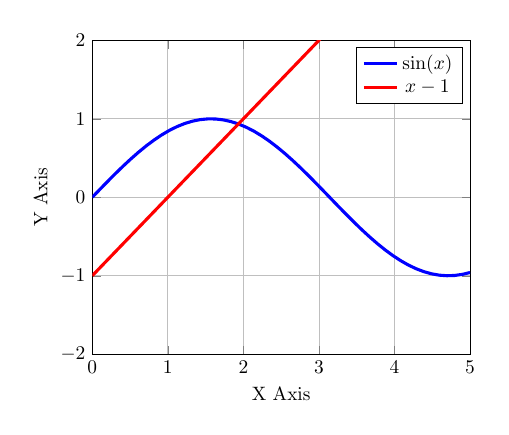
\begin{tikzpicture}[scale=0.7]
			\begin{axis}[
					xmax=5,
					xmin=0,
					ymax=2,
					ymin=-2,
					samples=50,
					grid=major,
					xlabel={X Axis},
					ylabel={Y Axis},
				]
				\addplot[blue, ultra thick,domain=0:5]{sin(deg(x))};
				\addplot[red, ultra thick,domain=0:5]{x-1};
				\legend{$\sin(x)$,$x-1$}
			\end{axis}
		\end{tikzpicture}
		\caption{Plot of the equation $\sin(x)=x-1$}
		\label{sketch:exm-continuous-opposite-signs:2}
	\end{figure}
\end{exm}

\begin{thm}\label{thm-intermediate-value-theorem}
	Let $f:[a,b]\to\mathbb{R}$ be a continuous function, and let $y_0$ be a value
	between $f(a)$ and $f(b)$. Then there exists an $x_0\in(a,b)$ such that
	\footnote{This a generalization of \pref{theorem}{thm-continuous-opposite-signs}}
	$f(x_0)=y_0$. \textit{Remark}: This theorem is also known as the intermediate
	value theorem.
\end{thm}

\begin{proof}
	Of \pref{theorem}{thm-intermediate-value-theorem}.
	\begin{flushleft}
		Assume \gls{wlog} that $f(a)<y_0<f(b)$. Then define $g(x)=f(x)-y_0$. By
		\pref{theorem}{thm-arithmetic-continuous} this function is also continuous on $[a,b]$.
		Therefore,
		\begin{align*}
			 & g(a)=f(a)-y_0<0, \\
			 & g(b)=f(b)-y_0>0
		\end{align*}
	\end{flushleft}
	By \pref{theorem}{thm-continuous-opposite-signs} there exists an $x_0$ such that
	$g(x_0)=0$. Therefore, $f(x_0)=y_0$.
\end{proof}

\begin{thm}\label{thm-weierstrass-theorems}
	Let $f:[a,b]\to\mathbb{R}$ be a continuous function. Weierstrass states the
	following two theorems:
	\begin{enumerate}
		\item The function $f$ is bounded.
		\item The function $f$ assumes a minimum and a maximum.
	\end{enumerate}
\end{thm}

\begin{thm}\label{thm-monotone-closed-interval}
	Let $f:[a,b]\to\mathbb{R}$ be a monotone function. Then, $f$ is continuous
	\textit{iff} the image of $f$ is a closed interval.
\end{thm}

\begin{proof}
	Of theorem (\ref{thm-monotone-closed-interval}).
	\begin{flushleft}
		By \pref{theorem}{thm-weierstrass-theorems}, statement 2, the function $f$
		assumes a minimum $m$ and maximum $M$. The image of $f$ is $[m,M]$ because
		$f$ obtains any value $y_0\in(m,M)$ by \pref{the intermediate value theorem}{thm-intermediate-value-theorem}.
	\end{flushleft}
\end{proof}

\begin{thm}\label{thm-continuous-monotone-invertible}
	If $f$ is continuous and strictly monotone, then $f$ is invertible whose
	inverse function is also continuous and monotone.
\end{thm}

% Single Variable Calculus
\section{Single Variable Calculus}

TODO: Add descriptions

\subsection{Derivatives}\label{subsec-derivatives}

\begin{definition}\label{def-differentiable}
	We say that a function $f$ is differentiable at $x_0$ if the limit in
	\pref{equation}{eq-differentiable} exists and is finite. The (first) derivative
	of $f$ at $x_0$ is equal to the result of this limit and is denoted by
	\begin{equation}\label{eq-differentiable}
		\lim_{x \to x_0}\frac{f(x)-f(x_0)}{x-x_0} \defines f^\prime(x_0) = \frac{\diff f}{\diff x}(x_0)
	\end{equation}
\end{definition}

\begin{rem}\label{rem-differentiable}
	The limit in \pref{definition}{def-differentiable} is equivalent to
	\begin{equation}\label{eq-differentiable-alt}
		f^\prime(x_0)=\lim_{h \to 0}\frac{f(x_0+h)-f(x_0)}{h}
	\end{equation}
	You can convince yourself that these definitions are equivalent by substituting
	$h\defines x-x_0$.
\end{rem}

\begin{definition}
	If $f$ is differentiable at $x_0$, then
	\begin{equation}
		y = f^\prime(x_0)(x-x_0)+f(x_0)
	\end{equation}
	is called the tangent line of $f$ at $x_0$.
\end{definition}

\begin{exm}\label{exm-derivatives:1}
	Let $f(x)=c$. For any $x_0\in\domain{f}$,
	\begin{align*}
		f^\prime(x_0) & = \lim_{x \to x_0}\frac{c-c}{x-x_0} \\
		              & = 0
	\end{align*}
\end{exm}

\begin{exm}\label{exm-derivatives:2}
	Let $f(x)=x$. For any $x_0\in\domain{f}$,
	\begin{align*}
		f^\prime(x_0) & = \lim_{x \to x_0}\frac{x-x_0}{x-x_0} \\
		              & = 1
	\end{align*}
\end{exm}

\begin{exm}\label{exm-derivatives:3}
	Let $f(x)=x^2$. For any $x_0\in\domain{f}$,
	\begin{align*}
		f^\prime(x_0) & = \lim_{x \to x_0}\frac{x^2-x_0^2}{x-x_0}      \\
		              & = \lim_{x \to x_0}\frac{(x-x_0)(x+x_0)}{x-x_0} \\
		              & = \lim_{x \to x_0} \left(x+x_0\right)          \\
		              & = 2x_0
	\end{align*}
\end{exm}

\begin{exm}\label{exm-derivatives:4}
	Let $f(x)=\sqrt{x}$. For any\footnote{This function in particular is not
		differentiable in the origin} $x_0\in\domain{f}:x_0>0$,
	\begin{align*}
		f^\prime(x_0) & = \lim_{x \to x_0}\frac{\sqrt{x}-\sqrt{x_0}}{x-x_0}                                               \\
		              & = \lim_{x \to x_0}\frac{(\sqrt{x}-\sqrt{x_0})(\sqrt{x}+\sqrt{x_0})}{(x-x_0)(\sqrt{x}+\sqrt{x_0})} \\
		              & = \lim_{x \to x_0}\frac{x-x_0}{(x-x_0)(\sqrt{x}+\sqrt{x_0})}                                      \\
		              & = \lim_{x \to x_0}\frac{1}{\sqrt{x}+\sqrt{x_0}}                                                   \\
		              & = \frac{1}{2\sqrt{x_0}}
	\end{align*}
\end{exm}

\begin{exm}\label{exm-derivatives:5}
	Let $f(x)=\sin(x)$. For any $x_0\in\domain{f}$,
	\begin{align*}
		f^\prime(x_0) & = \lim_{x \to x_0}\frac{\sin(x)-\sin(x_0)}{x-x_0}                                                                                                                                                               \\
		              & = \lim_{x \to x_0}\frac{2\sin\left(\frac{x-x_0}{2}\right)\cos\left(\frac{x+x_0}{2}\right)}{x-x_0}                                                                                                               \\
		              & = \lim_{x \to x_0}\left(\frac{\sin\left(\frac{x-x_0}{2}\right)}{\frac{x-x_0}{2}}\right)\lim_{x \to x_0}\left(\cos\left(\frac{x+x_0}{2}\right)\right) &  & \text{definition (\ref{thm-limit-arithmetic})}        \\
		              & = \cos(x_0)                                                                                                                                          &  & \text{example (\ref{exm-important-sin-over-x-limit})}
	\end{align*}
\end{exm}

\begin{rem}\label{rem-euler-limit}
	We can rewrite theorem (\ref{thm-euler-sequence-monotonicity-increasing}) as
	function, \textit{i.e.}
	\begin{equation}
		\exp(x)\defines\lim_{h \to 0}\left(1+hx\right)^\frac{1}{h}=e
	\end{equation}
\end{rem}

\begin{definition}\label{def-euler-alt}
	An alternative definition of the euler number defines that $e$ is the unique
	positive number for which $f(x_0)=\exp(x_0)$, and
	\begin{align}
		f'(x_0) & = \lim_{h\to0}\frac{f(x_0+h)-f(x_0)}{h}\nonumber                          \\
		        & = \lim_{h\to0}\frac{\exp(x_0+h)-\exp(x_0)}{h}         &  & x_0=0\nonumber \\
		        & = \lim_{h\to0}\frac{\exp(h)-1}{h}\label{eq-euler-alt}                     \\
		        & = 1\nonumber
	\end{align}
\end{definition}

\begin{exm}\label{exm-derivatives:6}
	Let $f(x)=\ln(x)$. For any $x_0\in\domain{f}$,
	\begin{align*}
		f^\prime(x_0) & = \lim_{h \to 0}\frac{\ln(x_0+h)-\ln(x_0)}{h}                                                                                                           \\
		              & = \lim_{h \to 0}\frac{\ln\left(\frac{x+h}{x_0}\right)}{h}                                                                                               \\
		              & = \ln\left(\lim_{h \to 0}\left(\left(1+\frac{h}{x_0}\right)^{\frac{1}{h}}\right)\right) &  & \text{\pref{theorem}{thm-elementary-functions-continuous}} \\
		              & = \ln\left(\exp\left(\frac{1}{x_0}\right)\right)                                        &  & \text{\pref{remark}{rem-euler-limit}}                      \\
		              & = \frac{1}{x_0}
	\end{align*}
\end{exm}

\begin{exm}\label{exm-derivatives:7}
	Let $f(x)=\abs{x}$. For $x=0$ this limit does not exists because
	\begin{align*}
		f^\prime(x_0) & = \lim_{x \to 0}\frac{\abs{x}-\abs{0}}{x-0} \\
		              & = \lim_{x \to 0}\frac{\abs{x}}{x}
	\end{align*}
	but notice that this limit doesn't exists since
	\begin{equation*}
		\lim_{x \to 0^+}\frac{x}{x} = 1 \neq -1 = \lim_{x \to 0^-}\frac{-x}{x}
	\end{equation*}
	wherefore the derivative of the absolute value function \gls{dne} in the origin.
\end{exm}

\begin{rem}
	In \pref{example}{exm-derivatives:6} we saw why functions are not differentiable
	at cusps.
\end{rem}

\begin{thm}\label{thm-differentiability-implies-continuity}
	If the function $f$ is differentiable at $x_0$, then $f$ is continuous at $x_0$.
\end{thm}

\begin{proof}
	Of \pref{theorem}{thm-differentiability-implies-continuity}.
	\begin{flushleft}
		One of the prerequisites of this theorem are that the limit stated in
		\pref{definition}{def-differentiable} exists. Therefore,
		\begin{align*}
			\lim_{x \to x_0}\left(f(x)-f(x_0)\right) & = \underbrace{\lim_{x \to x_0}\left(\frac{f(x)-f(x_0)}{x-x_0}\right)}_{=f^\prime(x_0)}\cdot\underbrace{\lim_{x \to x_0}(x-x_0)}_{=0}                                                     \\
			                                         & =  0                                                                                                                                 &  & \text{\pref{definition}{thm-limit-arithmetic}} \\
		\end{align*}
		But this means $f(x)\tolim{x}{x_0}0$.
		So, by \pref{definition}{def-continuity-at-point-a}, $f$ is continuous at
		the point $x_0$.
	\end{flushleft}
\end{proof}

\begin{rem}\label{rem-continuity-doesnt-imply-differentiability}
	It is very important to point out that the converse of \pref{theorem}{thm-differentiability-implies-continuity}
	is false, \textit{i.e.} continuity does not imply differentiability. See \pref{example}{exm-derivatives:6}
	why this couldn't possibly be true. However, if $f$ is not continuous, then $f$ is not differentiable, either.
\end{rem}

\begin{definition}\label{def-one-sided-derivatives}
	Similar to \pref{definition}{def-differentiable}, we can define one-sided derivatives by
	\begin{equation}\label{eq-right-sided-derivative}
		f_+^\prime(x)=\lim_{x \to x_0^+}\frac{f(x)-f(x_0)}{x-x_0}
	\end{equation}
	\begin{equation}\label{eq-left-sided-derivative}
		f_-^\prime(x)=\lim_{x \to x_0^-}\frac{f(x)-f(x_0)}{x-x_0}
	\end{equation}
	if the limit exists.
\end{definition}

\begin{thm}\label{thm-derivative-arithmetic}
	Let $f$ and $g$ be two differentiable functions, and $c\in\mathbb{R}$. Then
	\begin{enumerate}
		\item $(c\cdot f)^\prime(x_0) = c \cdot f^\prime(x_0)$
		\item $(f \pm g)^\prime(x_0) = f^\prime(x_0) \pm g^\prime(x_0)$
		\item $(f \cdot g)^\prime(x_0) = f^\prime(x_0) \cdot g(x_0) + g^\prime(x_0) \cdot f(x_0)$
		\item $\left(\tfrac{f}{g}\right)^\prime(x_0) = \tfrac{f^\prime(x_0)\cdot g(x_0) - g^\prime(x_0) \cdot f(x_0)}{g^2(x_0)}$ if $g(x_0)\neq0$
	\end{enumerate}
\end{thm}

\begin{proof}
	Of \pref{theorem}{thm-derivative-arithmetic}.
	\begin{flushleft}
		\textbf{Product Rule}:
		\begin{align*}
			(f \cdot g)^\prime(x_0) & = \lim_{h \to 0}\frac{f(x_0+h) g(x_0+h)-f(x_0) g(x_0)}{h}                                                           \\
			                        & = \lim_{h \to 0}\left(\frac{1}{h}\big( f(x_0+h) g(x_0+h) - f(x_0)(x_0+h) +f(x_0)(x_0+h) - f(x_0) g(x_0)\big)\right) \\
			                        & = \lim_{h \to 0}\left(g(x_0+h)\frac{f(x_0+h)-f(x_0)}{h}+f(x_0)\frac{g(x_0+h)-g(x_0)}{h}\right)                      \\
			                        & = g(x_0) \cdot f^\prime(x_0) + f(x_0) \cdot g^\prime(x_0)
		\end{align*}
		Notice that in the last step we used the fact that by \pref{theorem}{thm-differentiability-implies-continuity},
		$g$ is continuous which is an important detail required in this proof that explains why
		$g(x_0+h)\tolim{h}{0}g(x_0)$.
	\end{flushleft}
\end{proof}

\begin{thm}\label{thm-chain-rule}
	If $f$ is differentiable at $x_0$ and $g$ is differentiable at $f(x_a)$, then
	\begin{equation}\label{eq-chain-rule}
		(g \circ f)^\prime(x_0) = \underbrace{g^\prime(f(x_0))}_{\text{outer derivative}} \cdot \underbrace{f^\prime(x_0)}_{\text{inner derivative}}
	\end{equation}
	This is called the chain rule.
\end{thm}

\begin{thm}\label{thm-derivative-of-inverse-function}
	Let $y=f(x)$ be invertible, continuous at a neighborhood of $x_0$, and differentiable
	at $x_0$. Also assume that $f^\prime(x_0)\neq0$. Then $x=f^{-1}(y)$ is differentiable
	at $y_0=f(x_0)$, and
	\begin{equation}\label{eq-derivative-of-inverse-function}
		\left(f^{-1}\right)^\prime(y_0)=\frac{1}{f^\prime(x_0)}
	\end{equation}
\end{thm}

\begin{exm}\label{exm-derivative-of-inverse-function:1}
	We know that for all $x>0$, $(\ln(x))^\prime=\tfrac{1}{x}$. The inverse function
	of $y=\ln(x)$ is $x=e^y$. Hence, by \pref{theorem}{thm-derivative-of-inverse-function}
	we can write
	\begin{equation*}
		(e^y)^\prime = \frac{1}{\ln(x)^\prime} = \frac{1}{x^{-1}} = e^y
	\end{equation*}
	where we used the result obtained from \pref{example}{exm-derivatives:5}.
\end{exm}

\begin{exm}\label{exm-derivative-of-inverse-function:2}
	Let $f(x)=\sin(x)=y$ and $f^{-1}(x)=\arcsin(y)$. Hence, by
	\pref{theorem}{thm-derivative-of-inverse-function} we can write
	\begin{align*}
		(\arcsin(y))^\prime & = \frac{1}{\sin(x)^\prime}     \\
		                    & = \frac{1}{\cos(x)}            \\
		                    & = \frac{1}{\sqrt{1-\sin^2(x)}} \\
		                    & = \frac{1}{\sqrt{1-y^2}}
	\end{align*}
\end{exm}

\begin{exm}\label{exm-derivative-of-inverse-function:3}
	Let $f(x)=\tan(x)=y$ and $f^{-1}(x)=\arctan(y)$. Hence, by
	\pref{theorem}{thm-derivative-of-inverse-function} we can write TODO
\end{exm}

\begin{rem}\label{rem-first-derivative-polynomial}
	Let $f(x)=x^\alpha$ with $\alpha\in\mathbb{R}$ and $x>0$. Define
	$g(x)\defines \ln(f(x))$. By using the chain rule we get that
	\begin{equation}\label{eq-first-derivative-polynomial:1}
		g^\prime(x) = \frac{1}{f(x)} \cdot f^\prime(x)
	\end{equation}
	On the other hand,
	\begin{equation}\label{eq-first-derivative-polynomial:2}
		g(x) = \ln(x^\alpha) = \alpha\ln(x) \implies g^\prime(x) = \frac{\alpha}{x}
	\end{equation}
	So by \pref{equation}{eq-first-derivative-polynomial:1} and \pref{equation}{eq-first-derivative-polynomial:2},
	\begin{align*}
		\frac{1}{f(x)} \cdot f^\prime(x) = \frac{\alpha}{x} \implies f^\prime(x) = \alpha \cdot x^{\alpha-1}
	\end{align*}
\end{rem}

\subsection{Higher Order Derivatives}\label{subsec-higher-order-derivatives}

\begin{definition}\label{def-higher-order-derivatives}
	We define the $n$-th derivative by recursion as the $(n-1)$-th derivative of
	the function $f$ and denote it in Leibniz notation by
	\begin{equation}
		f^{(n)}(x) = \frac{\diff^n f}{\diff x^n}
	\end{equation}
	if $f$ is $n$-times differentiable.
\end{definition}

\begin{rem}
	The zeroth derivative of a function is just the original function.
\end{rem}

\begin{thm}\label{thm-higher-order-derivative-arithmetic}
	Let $f$ and $g$ be two differentiable functions, and $c\in\mathbb{R}$. Then
	\footnote{Recall that $\binom{n}{k}=\tfrac{n!}{k!(n-k)!}$}
	\begin{enumerate}
		\item $(c\cdot f)^{(n)}(x_0) = c \cdot f^{(n)}(x_0)$
		\item $(f \pm g)^{(n)}(x_0) = f^{(n)}(x_0) \pm g^{(n)}(x_0)$
		\item $(f \cdot g)^{(n)}(x_0) = \sum_{k=0}^n \binom{n}{k}f^{(k)}(x_0) \cdot g^{(k-1)}(x_0)$
	\end{enumerate}
	The third item in this list is also called Leibniz' formula.
\end{thm}

\begin{exm}
	Let $f(x)=x^2e^x$. Find the $9$-th derivative of this function.
	\begin{flushleft}
		\textbf{Answer}: By \pref{theorem}{thm-higher-order-derivative-arithmetic},
		we have that
		\begin{align*}
			(x^2e^x)^{(9)} & = \sum_{k=0}^9\binom{9}{k}(x^2)^{(k)}(e^x)^{(k)}                                                                                \\
			               & = \left(\binom{9}{0}x^2+\binom{9}{1}2x+\binom{9}{2}2\right)e^x &  & \text{\pref{example}{exm-derivative-of-inverse-function:1}} \\
			               & = \left(x^2+18x+72\right)e^x
		\end{align*}
	\end{flushleft}
\end{exm}

\subsubsection{Fermats Theorem for Extrema}\label{subsubsec-fermtas-theorem-extrema}

\begin{thm}\label{thm-fermats-theorem-extrema}
	Let $f(x)$ be a function defined on $(a,b)$ and let this function take on
	a maximum (or minimum) value at some point $c\in(a,b)$. Fermat's theorem for
	extrema states that if $f$ is differentiable, then
	\begin{equation}
		f^\prime(c)=0
	\end{equation}
\end{thm}

\begin{proof}
	Of \pref{theorem}{thm-fermats-theorem-extrema}.
	\begin{flushleft}
		\gls{wlog} assume that $x_0$ is a maximum. Since $f$ is differentiable
		we can write
		\begin{align*}
			f^\prime(x_0) & = \lim_{x \to x_0}\frac{f(x)-f(x_0)}{x-x_0}   \\
			              & = \lim_{x \to x_0^+}\frac{f(x)-f(x_0)}{x-x_0} \\
			              & = \lim_{x \to x_0^-}\frac{f(x)-f(x_0)}{x-x_0}
		\end{align*}
		Now consider all $x>x_0$; it follows that
		\begin{align}
			 & x-x_0>0\nonumber                                                                     \\
			\implies
			 & f(x)-f(x_0)\leq0\nonumber                                                            \\
			\implies
			 & \frac{f(x)-f(x_0)}{x-x_0}\leq0\nonumber                                              \\
			\implies
			 & \lim_{x \to x_0^+}\frac{f(x)-f(x_0)}{x-x_0}\leq0\label{eq-fermats-theorem-extrema:1}
		\end{align}
		Next consider where $x<x_0$; then
		\begin{align}
			 & x-x_0<0\nonumber                                                                     \\
			\implies
			 & f(x)-f(x_0)\leq0\nonumber                                                            \\
			\implies
			 & \frac{f(x)-f(x_0)}{x-x_0}\geq0\nonumber                                              \\
			\implies
			 & \lim_{x \to x_0^-}\frac{f(x)-f(x_0)}{x-x_0}\geq0\label{eq-fermats-theorem-extrema:2}
		\end{align}
		In summary, \pref{equation}{eq-fermats-theorem-extrema:1} and \pref{equation}{eq-fermats-theorem-extrema:2}
		imply that
		\begin{equation*}
			f^\prime(x_0)=0
		\end{equation*}
	\end{flushleft}
\end{proof}

\begin{rem}
	In high school we often used implicitly \pref{theorem}{thm-fermats-theorem-extrema}
	to find candidates for maxima and minima values. But this theorem doesn't find
	\textit{all} possible candidates. Take for instance the absolute value function.
	It obviously has a minimum in the origin, but Fermat's theorem for extrema is not
	going to pick up this candidate since $f(x)=\abs{x}$ is not differentiable at $x=0$.
	On the other side, this theorem may even yield candidates that neither maxima nor
	minima (take for instance $f(x)=x^3$ at $x=0$) so you have to use this theorem with
	caution. It is not by accident that these values are referred to as \enquote{candidates}.
	They may or may not promote to extrema depending on the actual function.
\end{rem}

\subsubsection{Rolle's Theorem}\label{subsubsec-rolles-theorem}

\begin{thm}\label{thm-rolles-theorem}
	Let $a,b\in\mathbb{R}$ where $a<b$. Let $f$ be a continuous in $[a,b]$ and
	differentiable in $(a,b)$ subject to the condition \cite[p.169]{wuest2009} that
	\begin{equation*}
		f(a)=f(b)
	\end{equation*}
	Then there exists a $c\in(a,b)$ such that
	\begin{equation}
		f^\prime(c)=0
	\end{equation}
\end{thm}

\begin{proof}
	Of theorem (\ref{thm-rolles-theorem}).
	\begin{flushleft}
		Since $f$ is continuous on $[a,b]$, by \pref{theorem}{thm-weierstrass-theorems}
		it has a minimum $m$ and a maximum $M$. If $m=M$, then $f$ must be a constant
		function in which case we are done (\textit{cf.} \pref{example}{exm-derivatives:1}).
		But if we rule out this possibility, then $m<M$ implies that at least one
		the these extrema is not obtained at the endpoints of this interval since the
		theorem assumes that $f(a)=f(b)$ but $f(m)\neq f(M)$. Denote the extrema
		that is not an endpoint by $c\in(a,b)$. Because the function is differentiable
		in $(a,b)$, by \pref{theorem}{thm-fermats-theorem-extrema} we know that $f^\prime(c)=0$.
	\end{flushleft}
\end{proof}

\subsubsection{Mean Value Theorem}\label{subsubsec-mean-value-theorem}

\begin{thm}\label{thm-mean-value-theorem}
	Let $a,b\in\mathbb{R}$ where $a<b$. Let $f$ be continuous in $[a,b]$ and
	differentiable in $(a,b)$. Then there exists a $c\in(a,b)$ such that
	\footnote{This is also known as Lagrange's theorem}
	\begin{equation}
		f^\prime(c)=\frac{f(b)-f(a)}{b-a}
	\end{equation}
\end{thm}

\begin{proof}
	Of \pref{theorem}{thm-mean-value-theorem}.
	\begin{flushleft}
		We define a new function $F$ such that
		\begin{equation*}
			F(x)=f(x)-\underbrace{\left(f(a)+\frac{f(b)-f(a)}{b-a}(x-a)\right)}_{\text{secant line}}
		\end{equation*}
		Then \pref{theorem}{thm-arithmetic-continuous}, $F$ is continuous on $[a,b]$
		because $f$ was also continuous. It's also differentiable on $(a,b)$ for
		precisely the same reason, \textit{cf.} \pref{theorem}{thm-derivative-arithmetic}.
		Notice also that $F(a)=F(b)=0$. So, by \pref{theorem}{thm-rolles-theorem} there
		exists a $c\in(a,b)$ such that $F^\prime(c)=0$. Then
		\begin{align*}
			F^\prime(c) & = f^\prime(c) - \frac{f(b)-f(a)}{b-a} \\
			            & = 0
		\end{align*}
		Hence,
		\begin{equation*}
			f^\prime(c)=\frac{f(b)-f(a)}{b-a}
		\end{equation*}
	\end{flushleft}
\end{proof}

\subsubsection{Cauchy's Theorem}\label{subsubsec-cauchys-theorem}

\begin{thm}\label{thm-cauchys-theorem}
	Let $f(x)$ and $g(x)$ be continuous in $[a,b]$ and differentiable in $(a,b)$.
	Assume that $\forall x\in(a,b)$, $g^\prime(x)=0$. Then Cauchy's theorem states
	that
	\begin{enumerate}
		\item $g(a)\neq g(b)$
		\item $\exists c\in(a,b)$ s.t.
		      \begin{equation}
			      \frac{f^\prime(x)}{g^\prime(x)}=\frac{f(b)-f(a)}{g(b)-g(a)}
		      \end{equation}
	\end{enumerate}
\end{thm}

\begin{thm}\label{thm-differentiable-constant-zero}
	Let $f$ be a differentiable function defined on $(a,b)$. The function is constant
	\textit{iff} for any $x\in(a,b)$, $f^\prime(x)=0$.
\end{thm}

\begin{proof}
	Of \pref{theorem}{thm-differentiable-constant-zero}.
	\begin{flushleft}
		\proofright: We already proved this direction in \pref{example}{exm-derivatives:1}.
	\end{flushleft}
	\begin{flushleft}
		\proofleft: \gls{wlog} take any two points $x,y\in(a,b)$ such that $a<x<y<b$.
		By \pref{theorem}{thm-mean-value-theorem} on $[x,y]$, there exists a point
		$c\in(x,y)$ such that
		\begin{equation*}
			f^\prime(c) = \frac{f(y)-f(x)}{y-x} = 0
		\end{equation*}
		Hence, $f(y)=f(x)$. Therefore, $f$ is a constant function.
	\end{flushleft}
\end{proof}

\begin{thm}\label{thm-differentiable-strictly-monotone}
	Let $f$ be a differentiable function on $(a,b)$. If $f^\prime(x)>0$ for any
	$x\in\domain{f}$, then $f$ is strictly monotonically increasing. Conversely,
	if $f^\prime(x)<0$, then $f$ is strictly monotonically decreasing.
\end{thm}

\begin{proof}
	Of \pref{theorem}{thm-differentiable-strictly-monotone}.
	\begin{flushleft}
		\gls{wlog}, take any $a<x<y<b$. By \pref{theorem}{thm-mean-value-theorem},
		there is a point $c\in[x,y]$ such that
		\begin{equation}
			\frac{f^\prime(x)}{g^\prime(x)}=\frac{f(b)-f(a)}{g(b)-g(a)}
		\end{equation}
		Since $f^\prime(c)>0$ it follows that $f(y)>f(x)$. Hence, by
		\pref{definition}{def-monotonicity}, $f$ is strictly monotonically increasing.
	\end{flushleft}
\end{proof}

\begin{rem}\label{rem-differentiable-strictly-monotone}
	The converse of \pref{theorem}{thm-differentiable-strictly-monotone} is false,
	\textit{i.e.} if $f$ is strictly monotonically increasing or decreasing, then its
	first derivative is either strictly positive or negative, respectively. Take for
	instance $f(x)=x^3$. This function is strictly increasing on the entire real line,
	but its derivative at $x=0$ is zero. But what we can say is that
	\begin{equation}\label{eq-differentiable-strictly-monotone}
		\left(f\text{ is differentiable } \implies f^\prime\geq0\right)
		\iff f\text{ is monotonically increasing}
	\end{equation}
\end{rem}

\begin{exm}\label{exm-differentiable-strictly-monotone}
	Let $f(x)=\arctan(x)$. This function is strictly increasing on $\mathbb{R}$,
	since $f^\prime(x)=\tfrac{1}{1+x^2}>0$ for all $x\in\mathbb{R}$. Next consider
	the function $g(x)=\tfrac{1}{x}$. Then $g^\prime(x)=-\tfrac{1}{x^2}<0$ for any
	$x\neq0$, so this function is strictly monotonically decreasing.
\end{exm}

\subsection{Curve Sketching}\label{subsec-curve-sketching}

\begin{definition}\label{def-local-minimum-maximum}
	A point $x_0$ is called a local minimum if $f(x) \geq f(x_0)$ for all $x$ in
	a neighborhood of $x_0$. Likewise, it is called a local maximum if $f(x) \geq f(x_0)$
	for all $x$ in a neighborhood of $x_0$.
\end{definition}

\begin{definition}\label{def-extrema}
	We will call $x_0$ a local extrema if $x_0$ is a local minimum or maximum.
\end{definition}

\begin{definition}\label{def-critical-point}
	We will call $x_0$ a critical point if $f^\prime(x_0)=0$ or $f$ is not differentiable
	at $x_0$.
\end{definition}

\begin{thm}\label{thm-first-derivative-test}
	Let $x_0$ be a critical point of $f$, and assume that $f$ is continuous at $x_0$
	and differentiable in a neighborhood of $x_0$, although possibly not differentiable
	at $x_0$ itself. Then the first derivative test states that
	\begin{enumerate}
		\item if $f^\prime(x_0)$ changes signs from minus to plus, then
		      $x_0$ is local minimum.
		\item if $f^\prime(x_0)$ changes signs from plus to minus, then
		      $x_0$ is local maximum.
		\item if $f^\prime(x_0)$ does not change signs, then $x_0$ is not an
		      extremum.
	\end{enumerate}
\end{thm}

\begin{thm}\label{thm-second-derivative-test}
	Let $x_0$ be a critical point of $f$, and assume that $f$ is differentiable twice
	at $x_0$. Then the second derivative test states that
	\begin{enumerate}
		\item if $f''(x_0)>0$, then $x_0$ is local minimum.
		\item if $f''(x_0)<0$, then $x_0$ is local maximum.
		\item if $f''(x_0)=0$, then this theorem doesn't reveal any additional
		      information about $x_0$
	\end{enumerate}
\end{thm}

\begin{thm}\label{thm-darboux-theorem}
	Let $f$ be a differentiable function on $[a,b]$ (with one-sided derivatives
	at the points of this interval, \textit{i.e.} $f_+^\prime(a)$ and $f_-^\prime(b)$
	exists) and let $c$ be value between $f_+^\prime(a)$ and $f_-^\prime(b)$.
	Then Darboux theorem\footnote{This is sort of an
		\hyperref[thm-intermediate-value-theorem]{intermediate value theorem}
		for derivatives.} states that there exists an $x_0$ such that $f'(x_0)=c$.
\end{thm}

\begin{crl}\label{crl-darboux-theorem}
	If $f$ is differentiable on $[a,b]$, then $f'$ may have points of infinite
	discontinuities (as they were defined in definition (\ref{def-infinite-discontinuity})).
\end{crl}

\begin{rem}\label{rem-darboux-theorem}
	The derivative of $f$ never can have removable or jump discontinuities without
	violating \hyperref[thm-darboux-theorem]{Darboux theorem}.
\end{rem}

\begin{exm}
	Consider the function
	\begin{equation*}
		f(x)=\begin{cases}
			\abs{x}^\frac{3}{2}\sin\left(\frac{1}{x}\right)\text{ if }x\neq0 \\
			0\text{ else }
		\end{cases}
	\end{equation*}
	Show that $f'$ is not continuous at $x=0$.
	\begin{flushleft}
		\textbf{Answer}: TODO
	\end{flushleft}
\end{exm}

\begin{thm}\label{thm-lhopitals-rule}
	Let $f$ and $g$ be two differentiable functions in a neighborhood of $x=a$,
	although possibly not in the neighborhood of $x$ itself. Assume that
	\begin{equation*}
		\lim_{x \to a}f(x)=\lim_{x \to a}g(x)=0
	\end{equation*}
	and that $g'(x)\neq0$ for all $x \neq a$ near $a$. Assume further that the limit
	\begin{equation*}
		\lim_{x \to a}\frac{f'(x)}{g'(x)}
	\end{equation*}
	exists. If all these conditions are met, then L'H{\^o}pital's rule says that
	\begin{equation}
		\lim_{x \to a}\frac{f(x)}{g(x)}=\lim_{x \to a}\frac{f'(x)}{g'(x)}
	\end{equation}
\end{thm}

\begin{rem}\label{rem-lhopitals-rule}
	In L'H{\^o}pital's rule we find many theorems bundled together that allow us
	under certain conditions to calculate limits of the form \enquote{$\tfrac{\infty}{\infty}$}
	or \enquote{$\tfrac{0}{0}$}.
\end{rem}

\begin{exm}\label{exm-lhopitals-rule:1}
	Consider the function $f(x)=\tfrac{\sin(x)}{x}$. Find the limit of $f$ as $x\to0$.
	\begin{flushleft}
		\textbf{Answer}: By \pref{theorem}{thm-lhopitals-rule} we get that
		\begin{align*}
			\lim_{x\to0}\frac{\sin(x)}{x} & = \lim_{x\to0}\frac{\cos(x)}{1} \\
			                              & = 1
		\end{align*}
	\end{flushleft}
	Note that this was much easier to find than in \pref{example}{exm-important-sin-over-x-limit}.
\end{exm}

\begin{exm}\label{exm-lhopitals-rule:2}
	Consider the function $f(x)=\tfrac{\ln(x)}{x-1}$. Find the limit of $f$ as $x\to1$.
	\begin{flushleft}
		\textbf{Answer}: By \pref{theorem}{thm-lhopitals-rule} we get that
		\begin{align*}
			\lim_{x\to1}\frac{\ln(x)}{x-1} & = \lim_{x\to1}\frac{\frac{1}{x}}{1} \\
			                               & = 1
		\end{align*}
	\end{flushleft}
\end{exm}

\begin{exm}\label{exm-lhopitals-rule:3}
	Consider the function $f(x)=\tfrac{\sin(x)-x}{\tan(x)-x}$. Find the limit of $f$ as $x\to0$.
	\begin{flushleft}
		\textbf{Answer}: By \pref{theorem}{thm-lhopitals-rule} we get that
		\begin{align*}
			\lim_{x\to0}\frac{\sin(x)-x}{\tan(x)-x} & = \lim_{x\to0}\frac{\cos(x)-1}{\frac{1}{\cos^2(x)}}                      \\
			                                        & = \lim_{x\to0}\frac{-\sin(x)}{-2\cdot\frac{1}{\cos^3(x)}\cdot(-\sin(x))} \\
			                                        & = -\frac{1}{2}
		\end{align*}
	\end{flushleft}
\end{exm}

\begin{exm}\label{exm-lhopitals-rule:4}
	Consider the function $f(x)=x\ln(x)$. Find the limit of $f$ as $x\to0^+$.
	\begin{flushleft}
		\textbf{Answer}: By \pref{theorem}{thm-lhopitals-rule} we get that
		\begin{align*}
			\lim_{x\to0^+}x^x & = \lim_{x\to0^+}\frac{\ln(x)}{\frac{1}{x}}         \\
			                  & = \lim_{x\to0^+}\frac{\frac{1}{x}}{-\frac{1}{x^2}} \\
			                  & = \lim_{x\to0^+}\left(-x\right)                    \\
			                  & = 0
		\end{align*}
	\end{flushleft}
\end{exm}

\begin{exm}\label{exm-lhopitals-rule:5}
	Consider the function $f(x)=x^x$. Find the limit of $f$ as $x\to0^+$.
	\begin{flushleft}
		\textbf{Answer}: By \pref{theorem}{thm-lhopitals-rule} we get that
		\begin{align*}
			\lim_{x\to0^+}x^x & = \lim_{x\to0^+}e^{\ln\left(x^x\right)}                                                  \\
			                  & = \lim_{x\to0^+}e^{x\ln(x)}             &  & \text{example (\ref{exm-lhopitals-rule:4})} \\
			                  & = 1
		\end{align*}
	\end{flushleft}
\end{exm}

\begin{definition}\label{def-convex-concave-functions}
	A function is called convex on $I$ if for all $x,y\in I$ the secant connecting
	the point $(x,f(x))$ to the point $(y,f(y))$ is above the graph. Conversely,
	a function is called concave if for all $x,y\in I$ the secant connecting
	the point $(x,f(x))$ to the point $(y,f(y))$ is below the graph.
\end{definition}

\begin{thm}\label{thm-convex-concave-first-derivative}
	Let $f$ be a differentiable function on $(a,b)$. Then
	\begin{enumerate}
		\item $f$ is convex \textit{iff} the graph is above the tangent line at any $x_0\in(a,b)$.
		\item $f$ is convex \textit{iff} $f'$ is increasing
		\item $f$ is concave \textit{iff} the graph is below the tangent line at any $x_0\in(a,b)$.
		\item $f$ is concave \textit{iff} $f'$ is decreasing
	\end{enumerate}
\end{thm}

\begin{thm}\label{thm-convex-concave-second-derivative}
	Let $f$ be a twice differentiable function on $(a,b)$. Then
	\begin{enumerate}
		\item $f$ is convex \textit{iff} $f''\geq0$
		\item $f$ is concave \textit{iff} $f''<0$
	\end{enumerate}
\end{thm}

\begin{thm}\label{thm-convex-minimum}
	Let $f$ be a convex differentiable function on $(a,b)$, and let $x_0$ be a
	critical point of $f$. Then $x_0$ is a minimum.
\end{thm}

\begin{thm}\label{thm-concave-maximum}
	Let $f$ be a concave differentiable function on $(a,b)$, and let $x_0$ be a
	critical point of $f$. Then $x_0$ is a maximum.
\end{thm}

\begin{definition}\label{def-point-of-inflection}
	We call $x_0$ a point of inflection of $f$ if $f$ is continuous at $x_0$,
	convex on one side of $x_0$ and concave on the other side of $x_0$.
\end{definition}

\begin{rem}\label{rem-point-of-inflection}
	Definition (\ref{def-point-of-inflection}) makes no claim with respect to
	$f''(x_0)=0$ being a satisfactory condition for points of inflection.
\end{rem}

\begin{definition}\label{def-vertical-asymptotes}
	We call $x=x_0$ a vertical asymptote if\footnote{It suffices to require only
		one one-sided limit to diverge to towards either minus or plus infinity}
	\begin{equation}\label{eq-vertical-asymptotes:1}
		\lim_{x \to x_0^+}f(x)= \pm\infty
	\end{equation}
\end{definition}

\begin{definition}\label{def-asymptotes}
	We call $y=ax+b$ an asymptote if
	\begin{equation}\label{eq-asymptotes}
		\lim_{x \to \pm\infty}\left(f(x)-(ax+b)\right)=0
	\end{equation}
\end{definition}

\begin{rem}\label{rem-asymptotes}
	Note that
	\begin{align*}
		f(x)-ax-b                                                                                              & \tolim{x}{\infty}0 \\
		\iff
		\underbrace{\frac{f(x)}{x}}_{\to a}-\underbrace{\frac{ax}{x}}_{\to a}-\underbrace{\frac{b}{x}}_{\to 0} & \tolim{x}{\infty}0
	\end{align*}
	So to find linear asymptotes we can use the following limits:
	\begin{equation}\label{rem-asymptotes:a}
		a = \lim_{x \to \pm\infty}\frac{f(x)}{x}
	\end{equation}
	\begin{equation}\label{rem-asymptotes:b}
		b = \lim_{x \to \pm\infty}\left(f(x)-ax\right)
	\end{equation}
\end{rem}

\begin{exm}\label{exm-curve-sketching}
	Consider the function
	\begin{equation}\label{eq-curve-sketching}
		f(x)=\sqrt[3]{x^2(3-x)}
	\end{equation}
	\begin{flushleft}
		\textbf{Curve Sketching}:
		\begin{enumerate}
			\item The first thing we want to do is to find the domain of the
			      function $f$, which in this case is rather easy: $\domain{f}=\left\{x\in\mathbb{R}\setbuild x\leq3\right\}$.
			\item After that we are interested in the continuity of $f$; since compositions of
			      elementary function are continuous on their entire domain, there is no issue here.
			\item Next we look for points of intersection with the $x$-axis:
			      \begin{align*}
				      f(x) = 0   & = \sqrt[3]{x^2(3-x)} \\
				      \implies x & = 0                  \\
				      \implies x & = 3
			      \end{align*}
			      So the points of intersections are $(0,0)$ and $(3,0)$.
			\item Now we look for the first derivative of $f$. It's easier to find
			      if we rewrite \pref{equation}{eq-curve-sketching} to
			      \begin{equation}\label{eq-curve-sketching:2}
				      f'(x)=x^{\frac{2}{3}}(3-x)^{\frac{1}{3}}
			      \end{equation}
			      Therefore,
			      \begin{equation}\label{eq-curve-sketching:3}
				      f'(x) = \frac{2}{3}x^{-\frac{1}{3}}(3-x)^{\frac{1}{3}} - x^{\frac{2}{3}}\cdot\frac{1}{3}(3-x)^{-\frac{2}{3}}
			      \end{equation}
			      Note that \pref{equation}{eq-curve-sketching:3} is neither defined at
			      $x=0$ nor at $x=3$.
			\item This time we use \pref{theorem}{thm-convex-concave-first-derivative}
			      to find candidates for convex and concave points, \textit{i.e.} if $f' \geq 0$, then
			      \begin{align*}
				      \frac{2}{3}x^{-\frac{1}{3}}(3-x)^{\frac{1}{3}}      & \geq x^{\frac{2}{3}}\cdot\frac{1}{3}(3-x)^{-\frac{2}{3}}                    \\
				      \iff
				      \frac{2}{3}\left(\frac{3-x}{x}\right)^{\frac{1}{3}} & \geq \frac{1}{3}\left(\frac{x}{3-x}\right)^{\frac{2}{3}} &  & \text{if }x>0 \\
				      \iff
				      2(3-x)                                              & \geq x                                                                      \\
				      \iff
				      6-2x                                                & \geq 3x                                                                     \\
				      \iff
				      2                                                   & \geq x
			      \end{align*}
			      So, in the domain $0<x<2$, $f'$ is non-negative. On the other side,
			      if $x<0$ we get that
			      \begin{align*}
				      2(3-x) & \leq x \\
				      \iff
				      2      & \leq x
			      \end{align*}
			      In this case this case we reach a contradictory statement, so no new
			      information was obtained at this step of the calculation. Finally, if
			      $f' \leq 0$ and $x < 0$, then $2 \leq x \neq 3$. In particular, $f'(x=2)=0$.
			\item This step is dedicated to finding the extrema (minimum and maximum)
			      of this function. We can use the results from step (3) to calculate
			      \begin{align*}
				       & x=0 \implies (0,0) \text{ is a local minimum}          &  & \text{\pref{theorem}{thm-convex-minimum}}  \\
				       & x=2 \implies (2,\sqrt[3]{4})\text{ is a local maximum} &  & \text{\pref{theorem}{thm-concave-maximum}}
			      \end{align*}
			\item Now we use \pref{theorem}{thm-second-derivative-test}, the second derivative test:
			      \begin{equation}\label{eq-curve-sketching:4}
				      f''(x) = -2x^{-\frac{4}{3}}(3-x)^{-\frac{5}{3}}
			      \end{equation}
			      Notice that \pref{equation}{eq-curve-sketching:4} is not defined on $x = 0$
			      and $x = 3$. Furthermore, observe that $f'' > 0$ for $x > 3$ and $f'' < 0$ for
			      $0 \neq x < 3$.
			\item Finally it's time to look for points of inflection; we can see
			      from the previous results that there exists only one point of inflection
			      at $x=3$. And because this function is continuous, there exists no vertical
			      asymptote (\textit{cf.} \pref{definition}{def-vertical-asymptotes}) in the
			      domain of $f$. Using \pref{remark}{rem-asymptotes} the linear asymptote ends up being
			      \begin{equation*}
				      y = -x + 1
			      \end{equation*}
			      Last but not least we summarize the information we gathered so
			      far to sketch the curve, see also \pref{figure}{sketch:exm-curve-sketching:1}
			      for the final result.
		\end{enumerate}
	\end{flushleft}
	\begin{figure}[ht!]
		\centering
		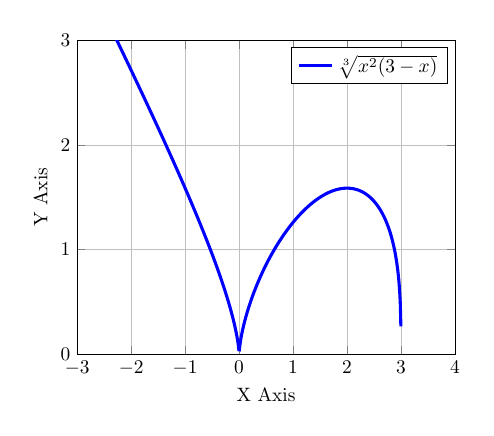
\begin{tikzpicture}[scale=0.7]
			\begin{axis}[
					xmax=4,
					xmin=-3,
					ymax=3,
					ymin=0,
					samples=1000,
					grid=major,
					xlabel={X Axis},
					ylabel={Y Axis},
				]
				\addplot[blue, ultra thick,domain=-5:5]{(x^2*(3-x))^(1/3)};
				\legend{$\sqrt[3]{x^2(3-x)}$}
			\end{axis}
		\end{tikzpicture}
		\caption{Final plot of curve from \pref{example}{exm-curve-sketching}}
		\label{sketch:exm-curve-sketching:1}
	\end{figure}
\end{exm}

\subsection{Taylor Polynomial}\label{subsec-taylor-polynomial}

Under certain conditions on $f$ near $x_0$ we will be able to find for any $\varepsilon>0$
a polynomial $p$ such that $f(x_0)=p(x_0)+R(x_0)$ where $R$ denotes the remainder ($\abs{R(x_0)}<\varepsilon$),
accounting for the inaccuracy of the approximation near $x_0$.

\begin{lemma}\label{lemma-polynomial-derivatives}
	Let $p_n(x)$ be a polynomial of degree $n$ of the function $f$ at the point $x$,
	such that
	\begin{equation}\label{eq-polynomial-derivatives:1}
		p_n(x) = \sum_{k=0}^n \beta_k x^k
	\end{equation}
	Then for any $k\in[0,n]$,
	\begin{equation}\label{eq-polynomial-derivatives:2}
		p_n^{(k)}(x) = \beta_k k!
	\end{equation}
\end{lemma}

\begin{proof}
	Of \pref{lemma}{lemma-polynomial-derivatives}.
	\begin{flushleft}
		If we differentiate the polynomial $p_n(x)$ $k$-times, then
		\begin{itemize}
			\item all terms of degree less than $k$ are zero
			\item for the $k$'th term ($\beta_k x^k$) we get $\beta_k k!$
			\item all terms of degree higher than $k$ disappear at $x=0$
		\end{itemize}
	\end{flushleft}
\end{proof}

\begin{rem}
	By the previous \pref{lemma}{lemma-polynomial-derivatives}, define the coefficients as
	\begin{equation*}
		\beta_k = \frac{p_n^{(k)}(x)}{k!}
	\end{equation*}
\end{rem}

\begin{definition}\label{def-taylor-polynomial}
	Let $n\in\mathbb{N}$ and $f$ be a $n$-times differentiable function at the point
	$x_0\in\domain{f}$. We call \cite[p.214]{wuest2009}
	\begin{equation}\label{eq-taylor-polynomial}
		p_n(f,x_0)(x) \defines \sum_{k=0}^n \frac{f^{(k)}(x_0)}{k!}(x-x_0)^k \qquad(x\in\mathbb{R})
	\end{equation}
	the Taylor polynomial of degree $n$ of the function $f$ at the point $x_0$.
\end{definition}

\begin{definition}\label{def-maclaurin-polynomial}
	The Taylor polynomial introduced in \pref{definition}{def-taylor-polynomial}
	is called Maclaurin polynomial, if $x_0=0$. So,
	\begin{equation}\label{eq-maclaurin-polynomial}
		p_n(f,0)(x) \defines \sum_{k=0}^n \frac{f^{(k)}(0)}{k!}x^k
	\end{equation}
\end{definition}

\begin{exm}\label{exm-sin-taylor-series}
	Find the Maclaurin polynomial for the function $f(x)=\sin(x)$ of degree $3$.
	\begin{flushleft}
		\textbf{Answer}: Since the Maclaurin polynomial evaluates at $x_0=0$,
		we find that
		\begin{align*}
			 & f(x)=\sin(x) \implies f(0)=0         \\
			 & f'(x)=\cos(x) \implies f'(0)=1       \\
			 & f''(x)=-\sin(x) \implies f''(0)=0    \\
			 & f'''(x)=-\cos(x) \implies f'''(0)=-1 \\
		\end{align*}
		So the polynomial is
		\begin{align*}
			p_3(\sin,0) & = f(0) + f'(0)x + \frac{f''(0)}{2!}x^2 + \frac{f'''(0)}{3!}x^3 \\
			            & = x - \frac{x^3}{3!}
		\end{align*}
	\end{flushleft}
	See \pref{figure}{sketch:taylor-polynomial:1} for an comparison between the
	original function and its approximation using the Maclaurin expansion.
	\begin{figure}[ht!]
		\centering
		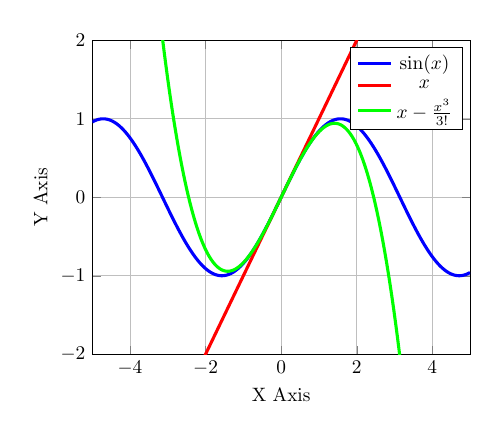
\begin{tikzpicture}[scale=0.7]
			\begin{axis}[
					xmax=5,
					xmin=-5,
					ymax=2,
					ymin=-2,
					samples=1000,
					grid=major,
					xlabel={X Axis},
					ylabel={Y Axis}]
				\addplot[blue, ultra thick,domain=-5:5]{sin(deg(x))};
				\addplot[red, ultra thick,domain=-5:5]{x};
				\addplot[green, ultra thick,domain=-5:5]{x-(x^3/3!)};
				\legend{$\sin(x)$,$x$,$x-\frac{x^3}{3!}$}
			\end{axis}
		\end{tikzpicture}
		\caption{Plot of the Taylor expansion for the function $\sin(x)$}
		\label{sketch:taylor-polynomial:1}
	\end{figure}
\end{exm}

\begin{exm}\label{exm-ln-taylor-series}
	Find the Maclaurin polynomial for the function $f(x)=\ln(x+1)$ of degree $n$.
	\begin{flushleft}
		\textbf{Answer}: Since the Maclaurin polynomial evaluates at $x_0=0$,
		we find that
		\begin{align*}
			 & f(x)=\ln(x+1) \implies f(0)=0                 \\
			 & f'(x)=\frac{1}{x+1} \implies f'(0)=1          \\
			 & f''(x)=-\frac{1}{(x+1)^2} \implies f''(0)=-1  \\
			 & f'''(x)=\frac{2}{(x+1)^3} \implies f'''(0)=-2 \\
		\end{align*}
		After a while it becomes easier to see that there is a pattern to this equation:
		\begin{align*}
			p_n(\ln(x+1),0) & = f(0) + f'(0)x + \frac{f''(0)}{2!}x^2 + \frac{f'''(0)}{3!}x^3 + \cdots + \frac{f^{(n)}(0)}{n!}x^n \\
			                & = x - \frac{x^2}{2} + \frac{x^3}{3} + \cdots + (-1)^{n+1}\frac{x^n}{n}                             \\
			                & = \sum_{k=1}^n (-1)^{k+1}\frac{x^k}{k}
		\end{align*}
	\end{flushleft}
\end{exm}

\begin{thm}\label{thm-taylor-lagrange-remainder-theorem}
	Let $f$ be a $n+1$-times differentiable function in a neighborhood of $x_0$,
	and let $x_0$ be a in that neighborhood. Then by Lagrange's remainder theorem
	there exists a point $\xi$ between $x_0$ and $x$ such that
	\begin{equation}\label{eq-taylor-lagrange-remainder-theorem}
		f(x) = p_n(f,x_0)(x) + \underbrace{\frac{f^{(n+1)}(\xi)}{(n+1)!}(x-x_0)^{n+1}}_{R_n(x)}
	\end{equation}
	where the error incurred by approximating $f$ is denoted by $R_n(x)$ and is
	called the remainder in Lagrange form.
\end{thm}

\begin{rem}
	For $n=0$ we get
	\begin{align*}
		f(x)             & = f(x_0) + f'(\xi)(x-x_0)   \\
		\implies f'(\xi) & = \frac{f(x)-f(x_0)}{x-x_0}
	\end{align*}
	So \hyperref[thm-mean-value-theorem]{the mean value theorem} is a special case
	of Lagrange's remainder theorem.
\end{rem}

\begin{exm}\label{exm-exp-taylor-series}
	The Maclaurin series of the exponential function can be easily found as
	\begin{equation*}
		p_n(\exp(x),0) = \sum_{k=0}^n \frac{x^k}{k!}
	\end{equation*}
	so we can approximate $f(x)=\exp(x)$ with a Taylor polynomial of degree $5$, \textit{i.e.}
	\begin{equation*}
		e^x = p_n(\exp(x),0) + R_n(x)
	\end{equation*}
	Now suppose we require $(\star)$ the remainder in Lagrange form to have at most an
	inaccuracy of $\tfrac{1}{100}$. Then there exists an $0<\xi<1$ and we can roughly
	estimate inaccuracy by
	\begin{align*}
		\abs{R_n(x)} & = \abs[\bigg]{\frac{e^\xi}{(n+1)!}}              \\
		             & = \frac{e^\xi}{(n+1)!}                           \\
		             & < \frac{e}{(n+1)!}                               \\
		             & < \frac{3}{(n+1)!}                               \\
		             & < \frac{1}{100}                     &  & (\star)
	\end{align*}
	Turns out that for $n=5$ the last inequality $(\star)$ holds. In fact, this
	estimation's inaccuracy was already found in the previous step to be $\tfrac{3}{6!}=\tfrac{1}{240}$.
\end{exm}

\begin{thm}\label{thm-infinite-taylor-lagrange-remainder-theorem}
	Let $f$ be a function differentiable infinitely many times in a neighborhood of $x_0$.
	Then there exists a constant $K$ such that for all $n\in\mathbb{N}$,
	\begin{equation}\label{eq-infinite-taylor-lagrange-remainder-theorem}
		\abs{f^{(n)}(x)} \leq K \implies R_n(x) \tolim{n}{\infty} 0
	\end{equation}
\end{thm}

\subsection{Indefinite Integrals}\label{subsec-indefinite-integrals}


\begin{definition}\label{def-indefinite-integral}
	The anti-derivative $F$ of a function $f$ on $I$ is defined such that
	\begin{equation}
		\forall x\in I:  F'(x) = f(x)
	\end{equation}
	When $F$ is an score of anti-derivative of $f$ we denote it by
	\begin{equation}\label{eq-indefinite-integral}
		\int f(x) \diff x = F(x) + C \qquad(C\in\mathbb{R})
	\end{equation}
	where the left-hand side of this equation describes an indefinite integral.
\end{definition}

\begin{exm}\label{exm-indefinite-integral:1}
	Find the indefinite integral of $\sin(x)$ with respect to $x$.
	\begin{flushleft}
		\textbf{Answer}: We can solve the immediate integral using the knowledge
		we obtained during our time when we studied derivatives of functions,
		\textit{i.e.}
		\begin{equation*}
			\int \sin(x) \diff x = -\cos(x) + C
		\end{equation*}
	\end{flushleft}
\end{exm}

\begin{exm}\label{exm-indefinite-integral:2}
	Find the indefinite integral of $x$ with respect to $x$.
	\begin{flushleft}
		\textbf{Answer}:
		\begin{equation*}
			\int x \diff x = -\frac{1}{2}x^2 + C
		\end{equation*}
	\end{flushleft}
\end{exm}

\begin{thm}\label{thm-indefinite-integral-linearity}
	Let $f$ and $g$ be two integrable functions, and let $\lambda\in\mathbb{R}$.
	Then indefinite integral satisfy the linearity property:
	\begin{enumerate}
		\item Addition:
		      \begin{equation}\label{eq-indefinite-integral-linearity:1}
			      \int \left(f(x)+g(x)\right) \diff x = \int f(x) \diff x + \int g(x) \diff x
		      \end{equation}
		\item Multiplication with a scalar:
		      \begin{equation}\label{eq-indefinite-integral-linearity:2}
			      \int \left(\lambda f(x)\right) \diff x = \lambda \int f(x) \diff x
		      \end{equation}
	\end{enumerate}
\end{thm}

\begin{exm}\label{exm-indefinite-integral:3}
	Find the indefinite integral of $\tfrac{x^4}{1+x^2}$ with respect to $x$.
	\begin{flushleft}
		\textbf{Answer}:
		\begin{align*}
			\int \frac{x^4}{1+x^2} \diff x & = \int \frac{x^4-1+1}{1+x^2} \diff x                                                                                \\
			                               & = \int \frac{(x^2-1)(x^2+1)+1}{1+x^2} \diff x                                                                       \\
			                               & = \int (x^2-1) \diff x + \int \frac{1}{1+x^2} \diff x &  & \text{\pref{theorem}{thm-indefinite-integral-linearity}} \\
			                               & = \frac{1}{3}x^3 - x + \arctan(x) + C
		\end{align*}
	\end{flushleft}
\end{exm}

\begin{exm}\label{exm-indefinite-integral:4}
	Find the indefinite integral of $\tan(x)$ with respect to $x$.
	\begin{flushleft}
		\textbf{Answer}: Note, that in general we have that
		\begin{equation}\label{eq-useful-integral}
			\int \frac{f'(x)}{f(x)} \diff x = \ln(\abs{f(x)}) + C \qquad(C\in\mathbb{R})
		\end{equation}
		which can be easily verified by taking the derivative on the right-hand side. Therefore,
		\begin{align*}
			\int \tan(x) \diff x & = \int \frac{\sin(x)}{\cos(x)} \diff x \\
			                     & = -\ln(\abs{\cos(x)}) + C
		\end{align*}
	\end{flushleft}
\end{exm}

\subsubsection{Integration by Parts}\label{subsubsec-integration-by-parts}

\begin{definition}\label{def-integration-by-parts}
	Using integration by parts we can integrate the product of two functions
	$u$,$v$ with respect to $x$ such that
	\begin{align*}
		\underbrace{\int \left(u(x)v(x)\right)' \diff x}_{u(x)v(x)} & = \int u'(x)v(x) \diff x + \int v'(x)u(x) \diff x &  & \text{\pref{definition}{thm-derivative-arithmetic}} \\
		\implies \int v'(x)u(x) \diff x                             & = u(x)v(x) - \int u'(x)v(x) \diff x
	\end{align*}
\end{definition}

\begin{exm}\label{exm-integration-by-parts:1}
	Use integration by parts to find the indefinite integral of $x\exp(x)$ with respect to $x$.
	\begin{flushleft}
		\textbf{Answer}: Let $u(x)=x$ and $v'(x)=\exp(x)$. Then,
		$u'(x)=1$ and $v(x)=\exp(x)$, thus
		\begin{align*}
			\int x\exp(x) \diff x & = x\exp(x) - \int 1\exp(x) \diff x \\
			                      & = \exp(x)\left(x-1\right) + C
		\end{align*}
	\end{flushleft}
\end{exm}

\begin{exm}\label{exm-integration-by-parts:2}
	Use integration by parts to find the indefinite integral of $\exp(x)\cos(x)$ with respect to $x$.
	\begin{flushleft}
		\textbf{Answer}: Let $u(x)=\cos(x)$ and $v'(x)=\exp(x)$. Then,
		$u'(x)=-\sin(x)$ and $v(x)=\exp(x)$, thus
		\begin{align*}
			\int \exp(x)\cos(x) \diff x           & = \exp(x)\cos(x) + \int \exp(x)\sin(x) \diff x                               \\
			                                      & = \exp(x)\cos(x) + \left(\exp(x)\sin(x) - \int \exp(x)\cos(x) \diff x\right) \\
			\implies 2\int \exp(x)\cos(x) \diff x & = \exp(x)\cos(x) + \exp(x)\sin(x) + C                                        \\
			                                      & = \frac{\exp(x)}{2}\big(\cos(x)+\sin(x)\big) + C
		\end{align*}
	\end{flushleft}
\end{exm}

\begin{exm}\label{exm-integration-by-parts:3}
	Use integration by parts to find the indefinite integral of $\arctan(x)$ with respect to $x$.
	\begin{flushleft}
		\textbf{Answer}: Note that $\arctan(x)=1\cdot\arctan(x)$. So, let
		$u(x)=\arctan(x)$ and $v'(x)=1$. Then, $u'(x)=\frac{1}{1+x^2}$ and $v(x)=x$, thus
		\begin{align*}
			\int \arctan(x) \diff x & = x\arctan(x) - \int \frac{x}{1+x^2} \diff x                                                    \\
			                        & = x\arctan(x) - \frac{1}{2}\ln(\abs{1+x^2}) + C &  & \text{\pref{equation}{eq-useful-integral}}
		\end{align*}
	\end{flushleft}
\end{exm}

\begin{exm}\label{exm-integration-by-parts:4}
	Find the indefinite integral of $\exp(-\abs{x})$ with respect to $x$.
	\begin{flushleft}
		\textbf{Answer}:
		\begin{align*}
			\int \exp(-\abs{x}) \diff x & = \begin{cases}
				\int \exp(-x) \diff x \text{ if } x\geq0 \\
				\int \exp(x) \diff x \text{ if } x<0     \\
			\end{cases}                    \\
			                            & \overset{(\star)}{=} \begin{cases}
				-\exp(-x) + 2 + C \text{ if } x\geq0 \\
				\exp(x) + C \text{ if } x<0
			\end{cases}
		\end{align*}
	\end{flushleft}
	Notice that we have to fix the discontinuity in $(\star)$ by adding $2$; see
	also \pref{figure}{sketch:exm-integration-by-parts:4}.
	\begin{equation*}
		\exp(-0)+C_1 = \exp(0) + C_2  \implies C_1 = 2 + C_2
	\end{equation*}
	If it weren't for this
	change the function would no longer be continuous (and by extension differentiable
	at $x=0$, \textit{cf.} \pref{remark}{rem-continuity-doesnt-imply-differentiability}),
	which in turn would violate \pref{definition}{def-indefinite-integral}.
	\begin{flushleft}
		\textbf{Left-hand side limit at $x=0$}:
		\begin{align*}
			F_-'(x_0) & = \lim_{h\to0^+}\frac{F(x_0+h)-F(x_0)}{h}                                                              \\
			          & = \lim_{h\to0^+}\frac{\exp(x_0+h)+C-(-\exp(-x_0)+2+C)}{h}                                              \\
			          & = \lim_{h\to0^+}\frac{\exp(x_0)\exp(h)+\exp(x_0)-2}{h}    &  & x_0 = 0                                 \\
			          & = \lim_{h\to0^+}\frac{\exp(h)-1}{h}                       &  & \text{\pref{definition}{def-euler-alt}} \\
			          & = 1
		\end{align*}
		\textbf{Right-hand side limit at $x=0$}:
		\begin{align*}
			F_+'(x_0) & = \lim_{h\to0^-}\frac{F(x_0+h)-F(x_0)}{h}                                                                 \\
			          & = \lim_{h\to0^-}\frac{\exp(-x_0-h)+2+C-(-\exp(-x_0)+2+C)}{h} &  & x_0 = 0                                 \\
			          & = \lim_{h\to0^-}\frac{-\exp(h)+1}{h}                         &  & \text{\pref{definition}{def-euler-alt}} \\
			          & = 1
		\end{align*}
	\end{flushleft}
	\begin{figure}[ht!]
		\centering
		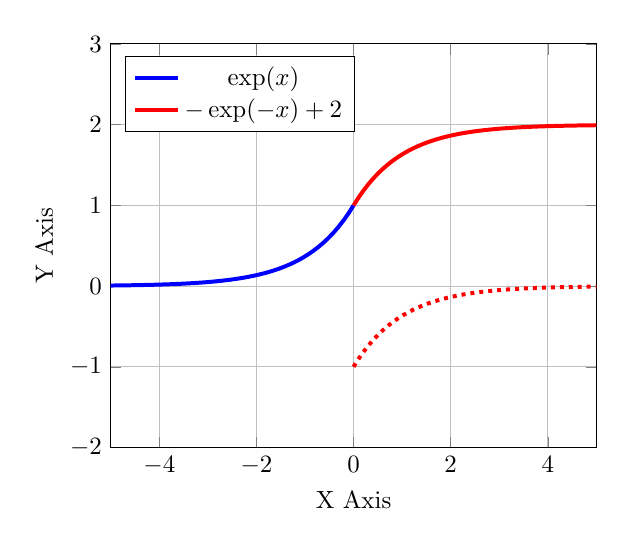
\begin{tikzpicture}[scale=0.9]
			\begin{axis}[
					xmax=5,
					xmin=-5,
					ymax=3,
					ymin=-2,
					samples=50,
					grid=major,
					xlabel={X Axis},
					ylabel={Y Axis},
					legend pos=north west
				]
				\addplot[blue,ultra thick,domain=-5:0]{exp(x)};
				\addplot[red,ultra thick,domain=0:5]{-exp(-x)+2};
				\addplot[red,ultra thick,dotted,domain=0:5]{-exp(-x)};
				\legend{$\exp(x)$,$-\exp(-x)+2$}
			\end{axis}
		\end{tikzpicture}
		\caption{Plot of the indefinite integral of $\exp(-\abs{x})$}
		\label{sketch:exm-integration-by-parts:4}
	\end{figure}
\end{exm}

\subsubsection{Integration of Rational Functions}\label{subsubsec-integration-rational-functions}

\begin{flushleft}
	Rational functions are of the form $\tfrac{p(x)}{q(x)}$ (where $p(x)$ and $q(x)$
	are polynomials and $q(x)\neq0$) that require different approaches when it
	comes to integration depending on the situation at hand. In this subsection
	we will walk through each case step by step by example, rather than proving
	the theorem that provides the underlying theory.
\end{flushleft}

\begin{exm}\label{exm-integration-rational-function:1}
	Find the indefinite integral of
	\begin{equation*}
		\int \frac{2x^4-x^3-x^2+3x-4}{x^2+1} \diff x
	\end{equation*}
	\begin{flushleft}
		\textbf{Answer}: In this example we have to first simplify the expression
		algebraically by performing a long division with polynomials\footnote{See
			also: \url{https://en.wikipedia.org/wiki/Polynomial_long_division}}, the
		result of which is
		\begin{align*}
			\int \frac{2x^4-x^3-x^2+3x-4}{x^2+1} \diff x
			 & = \int \left(2x^2-x-3+\frac{4x-1}{x^2-1}\right) \diff x                                                                                       \\
			 & = \frac{2}{3}x^3 -\frac{1}{2}x^2-3x + \int \frac{4x-1}{x^2-1} \diff x         &  & \text{\pref{example}{exm-integration-rational-function:4}} \\
			 & = \frac{2}{3}x^3 -\frac{1}{2}x^2-3x + \ln(\abs{3x-1}) + \frac{2}{3(3x-1)} + C
		\end{align*}
		\textit{This kind of situation occurs when $\deg(p)>\deg(q)$.}
	\end{flushleft}
\end{exm}

\begin{exm}\label{exm-integration-rational-function:2}
	Find the indefinite integral of
	\begin{equation*}
		\int \frac{1}{2x^2+9x-5} \diff x
	\end{equation*}
	\begin{flushleft}
		\textbf{Answer}: In this example we use \gls{pfd} to split up the integral
		into two parts\footnote{See also: \url{https://en.wikipedia.org/wiki/Partial_fraction_decomposition}}
		\begin{align*}
			\int \frac{1}{2x^2+9x-5} \diff x
			 & = \int \frac{1}{(2x-1)(x+5)} \diff x                                                                                              \\
			 & = \int \frac{A}{2x-1} \diff x + \int \frac{B}{x+5} \diff x                                                                        \\
			 & = \int \frac{\frac{2}{11}}{2x-1} \diff x + \int \frac{-\frac{1}{11}}{x+5} \diff x                                                 \\
			 & = \frac{1}{11}\int \frac{2}{2x-1} - \frac{1}{11} \int \frac{1}{x+5} \diff x       &  & \text{\pref{equation}{eq-useful-integral}} \\
			 & = \frac{1}{11}\ln(\abs{2x-1}) - \frac{1}{11}\ln(\abs{x+5}) + C
		\end{align*}
		\textit{This kind of situation occurs when the denominator $q$ has distinct
			linear factors.}
	\end{flushleft}
\end{exm}

\begin{exm}\label{exm-integration-rational-function:3}
	Find the indefinite integral of
	\begin{equation*}
		\int \frac{9x-5}{9x^2-6x+1} \diff x
	\end{equation*}
	\begin{flushleft}
		\textbf{Answer}: This type of integral is similar to the one we encountered
		in \pref{example}{exm-integration-rational-function:1}, but it has a little
		twist to it as can be observed in the solution below:
		\begin{align*}
			\int \frac{9x-5}{9x^2-6x+1} \diff x
			 & = \int \frac{9x-5}{(3x-1)^2} \diff x                                                                            \\
			 & = \int \frac{A}{3x-1} \diff x + \int \frac{B}{(3x-1)^2} \diff x                                                 \\
			 & = \int \frac{3}{3x-1} \diff x - \int \frac{2}{(3x-1)^2} \diff x &  & \text{\pref{equation}{eq-useful-integral}} \\
			 & = \ln(\abs{3x-1}) + \frac{2}{3}\cdot\frac{1}{3x-1} + C
		\end{align*}
		\textit{This kind of situation occurs when $q$ has a linear factor with
			multiplicity greater than or equal to $2$.}
	\end{flushleft}
\end{exm}

\begin{exm}\label{exm-integration-rational-function:4}
	Find the indefinite integral of
	\begin{equation*}
		\int \frac{4x-1}{x^2-1} \diff x
	\end{equation*}
	\begin{flushleft}
		\textbf{Answer}: This one is kind of weird, but it turns out to be not as
		involved as the previous examples once we recognize that we can force this
		integral into a form that is easier to solve:
		\begin{align*}
			\int \frac{4x-1}{x^2-1} \diff x
			 & = 2 \int \frac{2x}{x^2-1} \diff x - \int \frac{1}{x^2-1} \diff x &  & \text{\pref{equation}{eq-useful-integral}} \\
			 & = 2\ln(\abs{x^2-1}) - \arctan(x) + C
		\end{align*}
		\textit{This kind of situation occurs when $q$ has a quadratic irreducible
			factor does not break into linear factors.}
	\end{flushleft}
\end{exm}

\begin{exm}\label{exm-integration-rational-function:5}
	Find the indefinite integral of
	\begin{equation*}
		\int \frac{1}{x^2-x-1} \diff x
	\end{equation*}
	\begin{flushleft}
		\textbf{Answer}: This type of integral is of the set of problems as
		\pref{example}{exm-integration-rational-function:4}, but here we use a
		different approach: We use the identity
		\begin{equation}\label{eq-useful-square-identity}
			x^2 + px + q = \left(x+\frac{p}{2}\right)^2 + \left(q - \frac{p^2}{4}\right)
		\end{equation}
		So, the integral simplifies to
		\begin{align*}
			\int \frac{1}{x^2-x-1} \diff x
			 & = \int \frac{1}{\left(x-\frac{1}{2}\right)^2+\frac{3}{4}} \diff x                                           &  & \text{\pref{equation}{eq-useful-square-identity}} \\
			 & = \frac{4}{3} \int \frac{1}{\left(\frac{2}{\sqrt{3}}\left(x-\frac{1}{2}\right)\right)^2+1} \diff x                                                                 \\
			 & = \frac{4}{3} \cdot \frac{\sqrt{3}}{2} \arctan\left(\frac{2}{\sqrt{3}}\left(x-\frac{1}{2}\right)\right) + C                                                        \\
			 & = \frac{2\sqrt{3}}{3} \arctan\left(\frac{2}{\sqrt{3}}\left(x-\frac{1}{2}\right)\right) + C                                                                         \\
		\end{align*}
		\textit{This kind of situation occurs when $q$ has a quadratic irreducible
			factor does not break into linear factors.}
	\end{flushleft}
\end{exm}

\begin{exm}\label{exm-integration-rational-function:6}
	Find the indefinite integral of
	\begin{equation*}
		\int \frac{-x+2}{x^2-x+1} \diff x
	\end{equation*}
	\begin{flushleft}
		\textbf{Answer}: In this example we are still exploring the situation
		has a quadratic irreducible factor does not break into linear factors.
		\begin{align*}
			\int \frac{-x+2}{x^2-x+1} \diff x
			 & = -\frac{1}{2} \int \frac{2x-1}{x^2-x+1} \diff x + \frac{3}{2}\int \frac{1}{x^2-x+1} \diff x                      &  & \text{\pref{example}{exm-integration-rational-function:5}} \\
			 & = -\frac{1}{2}\ln(\abs{x^2-x-+1}) + \sqrt{3} \arctan\left(\frac{2}{\sqrt{3}}\left(x-\frac{1}{2}\right)\right) + C
		\end{align*}
		\textit{This kind of situation occurs when $q$ has a quadratic irreducible
			factor does not break into linear factors.}
	\end{flushleft}
\end{exm}

\begin{exm}\label{exm-integration-rational-function:7}
	Find the indefinite integral of
	\begin{equation*}
		\int \frac{1}{x^3+1} \diff x
	\end{equation*}
	\begin{flushleft}
		\textbf{Answer}: Finding the roots of polynomials of degree $3$ or higher is
		usually rather difficult, but in this example we can already see that $-1$ is
		a root of this polynomial. Therefore, we are in a position where we can use
		\gls{pfd} again to solve this integral:
		\begin{align*}
			\int \frac{1}{x^3+1} \diff x
			 & = \int \frac{1}{(x+1)(x^2-x=1)} \diff x                                                                                                                         \\
			 & = \int \frac{A}{x+1} \diff x + \int \frac{Bx+C}{x^2-x+1} \diff x                                                                                                \\
			 & = \int \frac{\frac{1}{3}}{x+1} \diff x + \int \frac{-\frac{1}{3}x+\frac{2}{3}}{x^2-x+1} \diff x                                                                 \\
			 & = \frac{1}{3} \frac{1}{x+1} \diff x + \frac{1}{3} \int \frac{-x+2}{x^2-x+1} \diff x             &  & \text{\pref{example}{exm-integration-rational-function:6}} \\
			 & = \frac{1}{3}\ln(\abs{x+1}) -\frac{1}{6}\ln(\abs{x^2-x-+1})                                                                                                     \\
			 & + \frac{1}{\sqrt{3}} \arctan\left(\frac{2}{\sqrt{3}}\left(x-\frac{1}{2}\right)\right) + C
		\end{align*}
		\textit{This kind of situation occurs when $\deg(q)=3$.}
	\end{flushleft}
\end{exm}

\subsubsection{Integration by Substitution}\label{subsubsec-integration-by-substitution}

\begin{thm}\label{thm-integration-using-substitution}
	If $x=\varphi(u)$ is differentiable and invertible, then the formula for
	substitution\footnote{Sometimes also called change of variables} is
	\begin{equation}\label{eq-integration-using-substitution}
		\int f(x) \diff x = \int f(\varphi(u))\varphi'(u) \diff u
	\end{equation}
\end{thm}

\begin{exm}\label{exm-integration-using-substitution:1}
	Use the substitution technique to find the indefinite integral of $\arctan(x)$ with respect to $x$.
	\begin{flushleft}
		\textbf{Answer}: Let $u \defines \exp(x)$. Then $\diff u = \exp(x) \diff x$, and
		\begin{align*}
			\int \frac{\exp(x)}{\exp(2x)+1} \diff x & = \int \frac{1}{u^2+1} \diff u \\
			                                        & = \arctan(\abs{u}) + C         \\
			                                        & = \arctan(\abs{\exp(x)}) + C
		\end{align*}
	\end{flushleft}
\end{exm}

\begin{exm}\label{exm-integration-using-substitution:2}
	Use the substitution technique to find the indefinite integral of $2x\exp(x^2)$ with respect to $x$.
	\begin{flushleft}
		\textbf{Answer}: Let $u \defines x^2$. Then $\diff u = 2x \diff x$, and
		\begin{align*}
			\int 2x\exp(x^2) \diff x & = \int \exp(u) \diff u \\
			                         & = \exp(u) + C          \\
			                         & = \exp(x^2) + C
		\end{align*}
	\end{flushleft}
\end{exm}

\begin{exm}\label{exm-integration-using-substitution:3}
	Use the substitution technique to find the indefinite integral of $\tfrac{\sqrt{x}}{x+1}$ with respect to $x$.
	\begin{flushleft}
		\textbf{Answer}: Let $u \defines \sqrt{x}$. Then $x = u^2$ and $\diff x = 2u \diff u$, so
		\begin{align*}
			\int \frac{\sqrt{x}}{x+1} \diff & = 2\int \frac{u^2+1-1}{u^2+1} \diff u                          \\
			                                & = 2 \left(\int 1 \diff u - \int \frac{1}{u^2+1} \diff u\right) \\
			                                & = 2u - 2\arctan(\abs{u}) + C                                   \\
			                                & = 2\sqrt{x} - 2\arctan(\sqrt{x}) + C
		\end{align*}
	\end{flushleft}
\end{exm}

\begin{exm}\label{exm-integration-using-substitution:4}
	Use the substitution technique to find the indefinite integral of $\tfrac{1}{\cos(x)}$ with respect to $x$.
	\begin{flushleft}
		\textbf{Answer}: Let $u \defines \tan\left(\tfrac{x}{2}\right)$. Then $x = 2\arctan(u)$
		and $\diff x = \tfrac{2}{1+u^2} \diff u$. Note that $u=\sqrt{\frac{1-\cos(x)}{1+\cos(x)}}$, so
		\begin{align*}
			u^2                       & = \frac{1-\cos(x)}{1+\cos(x)} \\
			\implies u^2 + u^2\cos(x) & = 1 - \cos(x)                 \\
			\implies \cos(x)          & = \frac{1-u^2}{1+u^2}
		\end{align*}
		Therefore the integral becomes
		\begin{align*}
			\int \frac{1}{\cos(x)} \diff x & = \int \frac{1+u^2}{1-u^2} \cdot \frac{2}{1+u^2} \diff u                                                  \\
			                               & = \int \frac{2}{1-u^2} \diff u                                                                            \\
			                               & = \int \frac{1}{1-u} \diff u + \int \frac{1}{1+u} \diff u                                                 \\
			                               & = -\ln(\abs{1-u}) + \ln(\abs{1+u}) + C                                                                    \\
			                               & = -\ln\left(\abs[\Bigg]{\frac{1+\tan\left(\frac{x}{2}\right)}{1-\tan\left(\frac{x}{2}\right)}}\right) + C \\
		\end{align*}
	\end{flushleft}
\end{exm}

\subsection{Definite Integrals}\label{subsec-definite-integrals}

\begin{definition}\label{def-partition-of-an-interval}
	A partition of an interval $[a,b]$ on $\mathbb{R}$ is a finite sequence
	$x_0,x_1,\dots,x_n$ of real numbers such that
	\begin{equation}\label{eq-partition-of-an-interval}
		a = x_0 < x_1 < \dots < x_n = b
	\end{equation}
	and is denoted by $P$.
\end{definition}

\begin{definition}\label{def-max-partition}
	The biggest interval of the partition is defined by
	\begin{equation}\label{eq-max-partition}
		\lambda(P) \defines \max\left\{\Delta x_i \setbuild i\in\mathbb{N}\right\}
	\end{equation}
\end{definition}

\begin{definition}\label{def-riemann-sum}
	Let $P$ be a partition of $[a,b]$, and let $f:[a,b]\to\mathbb{R}$ be bounded.
	Choose points $x_i^*\in[x_{i-1},x_i]$ for $i\in\mathbb{N}$. Then
	\begin{equation}\label{eq-riemann-sum}
		\sum_{i=1}^n f(x_i^*)(x_i-x_{i-1}) = \sum_{i=1}^n f(x_i^*)\Delta x
	\end{equation}
	is called the Riemann sum for $f$ determined by the partition $P$.
\end{definition}

\begin{definition}\label{def-riemann-integrable}
	Let $f:[a,b]\to\mathbb{R}$ be bounded. We say that $f$ is a Riemann integrable
	function on $[a,b]$ if there exists an $I\in\mathbb{R}$ such that
	\begin{equation}
		\bigwedge_{\varepsilon>0}\bigvee_{\delta>0}\bigwedge_{\lambda(P)<\delta}
		\abs[\Bigg]{\sum_{i=1}^n f(x_i^*)\Delta x_i - I}<\varepsilon
	\end{equation}
	for all $x_i^*$.
\end{definition}

\begin{definition}\label{def-definite-integral}
	For a continuous function and bounded function $f:[a,b]\to\mathbb{R}$,
	the Riemann sum can by computed by
	\begin{equation}\label{eq-definite-integral}
		\int_a^b f(x) \diff x = \lim_{n\to\infty}\sum_{i=1}^n f(x_i^*)\Delta x
	\end{equation}
	for any choice of the $x_i^*\in[x_{i-1},x_i]$ with $\delta x = \tfrac{b-a}{n}$
	and $x_i = a + (i-1)\Delta x_i$, \textit{i.e.} $P$ partitions the interval $[a,b]$
	into subintervals of equal length\footnote{which are also called regular intervals}.
\end{definition}

\begin{rem}\label{rem-definite-integral}
	To determine the value of $x_i$, we use the formula
	\begin{enumerate}
		\item Left-Hand Rule: $\sum_{i=1}^n f(x_i)\Delta x$
		\item Midpoint Rule: $\sum_{i=1}^n f(x_{i+1})\Delta x$
		\item Right-Hand Rule: $\sum_{i=1}^n f\left(\frac{x_i+x_{i+1}}{2}\right)\Delta x$
	\end{enumerate}
\end{rem}

\begin{exm}\label{exm-riemann-sum:1}
	Consider the constant function $f(x)=c$ on the interval $[a,b]$. For any $P$
	and choice off $c_i$ we get
	\begin{align*}
		\sum_{i=1}^n c \Delta x & = c \sum_{i=1}^n \Delta x \\
		                        & = c (b-a)
	\end{align*}
	Hence,
	\begin{equation*}
		\int_a^b c \diff x = c(b-a)
	\end{equation*}
\end{exm}

\begin{exm}\label{exm-riemann-sum:2}
	Consider the linear function $f(x)=x$ on the interval $[0,1]$. For any $P$
	and choice off $c_i$ we partition the interval into subintervals of length $n$
	using the right-hand rule, so $\Delta x = \frac{1}{n}$, and
	\begin{equation*}
		x_i = 0 + ((i+1)-1)\Delta x = \frac{i}{n}
	\end{equation*}
	Then the Riemann sum of this function is
	\begin{align*}
		\sum_{i=1}^n f(x_{i+1}) \Delta x & = \sum_{i=1}^n f\left(\frac{i}{n}\right)\Delta x \\
		                                 & = \frac{1}{n^2} \sum_{i=1}^n i                   \\
		                                 & = \frac{1}{n^2} \cdot \frac{n(n+1)}{2}           \\
		                                 & = \frac{n+1}{2n}
	\end{align*}
	Hence,
	\begin{equation*}
		\int_0^1 x \diff x = \lim_{n\to\infty}\frac{n+1}{2n} = \frac{1}{2}
	\end{equation*}
\end{exm}

\begin{exm}\label{exm-riemann-sum:3}
	Compute the Riemann sum of $f(x)=4x-x^2$ on $[0,4]$ with regular partitions
	$16$ using the left and right-hand rule from \pref{remark}{rem-definite-integral}.
	\begin{flushleft}
		\textbf{Answer}: Note that $a=0$ and $b=4$. From \pref{definition}{def-definite-integral}
		we have that for the right-hand rule,
		\begin{align*}
			\Delta x & = \frac{4-0}{16} = \frac{1}{4}      \\
			x_i      & = 0 + ((i+1)-1)\Delta x = i\Delta x
		\end{align*}
		Using the left-hand rule we get
		\begin{align*}
			\sum_{i=1}^{16} f(x_{i+1})\Delta x & = \sum_{i=1}^{16} f(i\Delta x)\Delta x                               \\
			                                   & = \sum_{i=1}^{16} \left(4 i \Delta x - i^2 \Delta x^2\right)\Delta x \\
			                                   & = 4 \Delta x^2 \sum_{i=1}^{16} i - \Delta x^3 \sum_{i=1}^{16} i^2    \\
			                                   & = 10.625
		\end{align*}
	\end{flushleft}
\end{exm}

\begin{rem}
	If $I\defines \int_a^b f(x) \diff x$ in \pref{definition}{def-definite-integral}
	exists, then it is unique.
\end{rem}

\begin{definition}\label{def-definite-integral-properties}
	The following properties of the definite integral can be deduced from the
	Riemann sum approach to integration:
	\begin{enumerate}
		\item Additive properties:
		      \begin{align}
			      \int_a^c f(x) \diff x & = \int_a^b f(x) \diff x + \int_b^c f(x) \diff x \\
			      \int_a^a f(x) \diff x & = 0                                             \\
			      \int_a^b f(x) \diff x & = -\int_b^a f(x) \diff x
		      \end{align}
	\end{enumerate}
\end{definition}

\begin{thm}\label{thm-continuous-monotone-integrable}
	If $f$ is piecewise continuous or piecewise monotone, then $f$ is (Riemann)
	integrable.
\end{thm}

\begin{thm}\label{thm-definite-integral-theorems}
	Let $f:[a,b]\to\mathbb{R}$ be a bounded function.
	\begin{enumerate}
		\item If $f$ is integrable on $[a,b]$, then it is integrable on any $[c,d]\subseteq[a,b]$.
		\item If $f$ and $g$ are integrable on $[a,b]$ and $\alpha,\beta\in\mathbb{R}$, then $\alpha f(x)+ \beta g(x)$ is integrable, and
		      \begin{equation}\label{eq-definite-integral-linearity}
			      \int_a^b \left(\alpha f(x)+ \beta g(x)\right) \diff x = \alpha \int_a^b f(x) \diff x + \beta \int_a^b g(x) \diff x
		      \end{equation}
		\item If $f$ and $g$ are integrable on $[a,b]$, then $(f \circ g)(x)$ is also integrable.
		\item If $f$ is integrable on $[a,b]$, then so is $\abs{f}$, and the following inequality holds:
		      \begin{equation}\label{eq-definite-integral-triangle-inequality}
			      \abs[\Bigg]{\int_a^b f(x) \diff x} \leq \int_a^b \abs{f(x)} \diff x
		      \end{equation}
		\item If $f$ is integrable on $[a,b]$ and $f(x)\geq0$ for every $x\in\domain{f}$, then\footnote{If $f(x_0)>0$ for some $x_0$,
			      $\int_a^b f(x) \diff x$ need not to strictly greater than zero. However, one can correct this by demanding continuity for $f$.}
		      \begin{equation}\label{eq-definite-integral-positvity}
			      \int_a^b f(x) \diff x \geq 0
		      \end{equation}
		\item If $f$ and $g$ are integrable on $[a,b]$ and $f(x)\geq g(x)$ for all $x\in\domain{f}$, then
		      \begin{equation}\label{eq-definite-integral-monotonicity}
			      \int_a^b f(x) \diff x \geq \int_a^b g(x) \diff x
		      \end{equation}
		\item If $f$ is integrable on $[a,b]$ and $m \leq f(x) \leq M$ for all $x\in\domain{f}$, then
		      \begin{equation}\label{eq-definite-integral-bounded}
			      m(b-a) \leq \int_a^b f(x) \diff x \leq M(b-a)
		      \end{equation}
		\item If $f$ is integrable on $[a,b]$ and continuous, there exists a $c\in[a,b]$ such that
		      \footnote{This is also called the intermediate value theorem for integrals, \textit{cf.} \pref{theorem}{thm-intermediate-value-theorem}}
		      \begin{equation}\label{eq-intermediate-value-theorem-for-theorems}
			      \int_a^b f(x) \diff x = f(c)(b-a)
		      \end{equation}
		\item If $f$ is integrable on $[a,b]$ and $\tilde{f}$ differs from $f$ at finitely many points, then $\tilde{f}$ is integrable and
		      \begin{equation}\label{eq-change-points-retain-integral}
			      \int_a^b f(x) \diff x =  \int_a^b \tilde{f}(x) \diff x
		      \end{equation}
	\end{enumerate}
\end{thm}

\begin{proof}
	Of \pref{equation}{eq-intermediate-value-theorem-for-theorems} in \pref{theorem}{thm-definite-integral-theorems}.
	\begin{flushleft}
		By \pref{equation}{eq-definite-integral-bounded} we know that
		\begin{equation*}
			m(b-a) \leq \int_a^b f(x) \diff x \leq M(b-a)
		\end{equation*}
		Then this implies
		\begin{align*}
			m \leq \frac{1}{b-a}\int_a^b f(x) \diff x \leq M
		\end{align*}
		So, by the intermediate value \pref{theorem}{thm-intermediate-value-theorem},
		there exists a $c$ such that
		\begin{equation*}
			f(c) =  \frac{1}{b-a}\int_a^b f(x) \diff x
		\end{equation*}
	\end{flushleft}
\end{proof}

\begin{thm}\label{thm-integrable-continuous}
	If $f$ is integrable on $[a,b]$, then
	\begin{equation}
		F(x) = \int_a^x f(t) \diff t
	\end{equation}
	is continuous on $[a,b]$.
\end{thm}

\subsubsection{The Fundamental Theorem of Calculus}\label{subsubsec-the-fundamental-theorem-of-calculus}

\begin{thm}\label{thm-the-fundamental-theorem-of-calculus}
	Suppose that $f:[a,b]\to\mathbb{R}$ is continuous. Define
	\begin{equation*}
		F(x) = \int_a^x f(t) \diff t
	\end{equation*}
	Then $F$ is differentiable. Moreover,
	\begin{equation}
		F'(x) = f(x)
	\end{equation}
\end{thm}

\begin{proof}
	Of \pref{theorem}{thm-the-fundamental-theorem-of-calculus}.
	\begin{flushleft}
		For any $x_0\in[a,b]$,
		\begin{align*}
			F_+'(x_0) & = \lim_{x \to x_0^+} \frac{F(x)-F(x_0)}{x-x_0}                                       &  & \text{\pref{theorem}{thm-integrable-continuous}}                   \\
			          & = \lim_{x \to x_0^+} \frac{\int_a^x f(t) \diff t - \int_a^{x_0} f(t) \diff t}{x-x_0}                                                                         \\
			          & = \lim_{x \to x_0^+} \frac{\int_{x_0}^x f(t) \diff t}{x-x_0}                         &  & \text{\pref{equation}{eq-intermediate-value-theorem-for-theorems}} \\
			          & = \lim_{x \to x_0^+} \frac{f(c_x)(x-x_0)}{x-x_0}                                                                                                             \\
			          & = \lim_{x \to x_0^+} f(c_x)                                                          &  & \text{\pref{definition}{def-continuity-at-point-a}}                \\
			          & = f(x_0)
		\end{align*}
	\end{flushleft}
\end{proof}

\begin{crl}\label{crl-continuity-implies-anti-derivative}
	Every continuous function has an anti-derivative.
\end{crl}

\begin{rem}\label{rem-continuity-implies-anti-derivative}
	Although the anti-derivative is not always an elementary function.
\end{rem}

\begin{crl}\label{crl-newton-leibniz-formula}
	Let $f:[a,b]\to\mathbb{R}$ be continuous and let $F(x)$ be an anti-derivative
	of $f$. Then
	\begin{equation}\label{eq-newton-leibniz-formula}
		\int_a^b f(x) \diff x = F(b) - F(a) = \evalat{F}{a}{b}
	\end{equation}
\end{crl}

\begin{exm}\label{exm-newton-leibniz-formula:1}
	Find the definite integral of
	\begin{equation*}
		f(x) = 2 + \cos(x) - \frac{x^2}{2}
	\end{equation*}
	from $0$ to $\tfrac{\pi}{2}$ with respect to $x$.
	\begin{flushleft}
		\textbf{Answer}:
		\begin{align*}
			\int_0^{\frac{\pi}{2}} f(x) \diff x & = \evalat{\left(2x+\sin(x)-\frac{x^3}{3}\right)}{0}{\frac{\pi}{2}}                                       \\
			                                    & = \left(2\cdot\frac{\pi}{2}+\sin\left(\frac{\pi}{2}\right)-\frac{\left(\frac{\pi}{2}\right)^3}{3}\right)
			- \left(2\cdot0+\sin(0)-\frac{0^3}{3}\right)                                                                                                   \\
			                                    & = \pi+1-\frac{\pi^3}{24}
		\end{align*}
	\end{flushleft}
\end{exm}

\begin{proof}
	Of \pref{corollary}{crl-newton-leibniz-formula}.
	\begin{flushleft}
		Define $G(x)=\int_a^x f(t) \diff t$. By \pref{theorem}{thm-the-fundamental-theorem-of-calculus},
		$G'(x)=f(x)$. Hence, there exists a constant $C\in\mathbb{R}$ such that $F(x)=G(x)+C$.
		Therefore,
		\begin{align*}
			F(b) - F(a) & = (G(b)+c) - (G(a)+c)                                                                                           \\
			            & = G(b) - G(a)                                                                                                   \\
			            & = \int_a^b f(x) \diff x - \int_a^a f(x) \diff x &  & \text{\pref{definition}{def-definite-integral-properties}} \\
			            & = \int_a^b f(x) \diff x
		\end{align*}
	\end{flushleft}
\end{proof}

\begin{exm}\label{exm-newton-leibniz-formula:2}
	Evaluate the following expression:
	\begin{equation*}
		\lim_{x\to0}\frac{1}{x^3}\int_0^x \sin^2(3t) \diff t
	\end{equation*}
	\begin{flushleft}
		\textbf{Answer}:
		\begin{align*}
			\lim_{x\to0}\frac{1}{x^3}\int_0^x \sin^2(3t) \diff t
			 & = \lim_{x\to0}\frac{\int_0^x \sin^2(3t) \diff t}{x^3} &  & \text{\pref{theorem}{thm-lhopitals-rule}, (\ref{thm-the-fundamental-theorem-of-calculus})} \\
			 & = \lim_{x\to0}\frac{3\sin^2(3x)}{3\cdot3x^2}          &  & \text{\pref{equation}{eq-important-sin-over-x-limit}}                                      \\
			 & = 1
		\end{align*}
	\end{flushleft}
\end{exm}

\begin{exm}\label{exm-newton-leibniz-formula:3}
	Let $G(x)=\int_0^{x+x^2}\sin(t)\diff t$. Find the first derivative of $G$.
	\begin{flushleft}
		\textbf{Answer}: By \pref{theorem}{thm-the-fundamental-theorem-of-calculus},
		that
		\begin{equation*}
			F(x)=\int_0^{x}\sin(t)\diff t \implies G'(x) = \sin(x)
		\end{equation*}
		Note that $G(x)=F(x+x^2)$, so
		\begin{align*}
			G'(x) & = F'(x+x^2)(1+2x)   \\
			      & = \sin(x+x^2)(1+2x)
		\end{align*}
	\end{flushleft}
\end{exm}

\begin{rem}\label{rem-newton-leibniz-formula}
	The implication below makes sense when $f$ is continuous, but when we drop this
	condition we will suddenly see that there are integrable function that are not
	continuous - take, for instance, the function
	\begin{equation*}
		f(x) = \begin{cases}
			1\text{ if } x\geq0 \\
			0\text{ else }
		\end{cases}
	\end{equation*}
	Obviously, $f(x)$ is piecewise integrable because it is piecewise continuous,
	but it doesn't have an anti-derivative on the entire interval since it has a
	jump discontinuity in the origin. So, it is not continuous at $x=0$ which
	violates \pref{definition}{def-indefinite-integral}. Therefore, in general
	\begin{equation}\label{eq-rem-newton-leibniz-formula:ltr}
		\text{$f$ is integrable} \notimplies \text{$f$ has an anti-derivative}
	\end{equation}
	Conversely, the other direction also doesn't hold:
	\begin{equation}\label{eq-rem-newton-leibniz-formula:rtl}
		\text{$f$ has an anti-derivative} \notimplies \text{$f$ is integrable}
	\end{equation}
	A function can be unbounded but still have an anti-derivative; but if the
	function is not bounded, then it is not integrable. For example, the function
	\begin{equation*}
		f:(0,1)\to\mathbb{R},x\mapsto\frac{1}{x}
	\end{equation*}
	is not bounded, which is why it is not integrable. This is the reason why we
	demand continuity in the fundamental theorem of \pref{calculus}{thm-the-fundamental-theorem-of-calculus}.
\end{rem}

\subsubsection{Integration by Parts}\label{subsubsec-integration-by-parts-definite-integrals}

\begin{thm}\label{thm-integration-by-parts-definite-integrals}
	If $u(x)$ and $v(x)$ have continuous derivatives on $[a,b]$ (\textit{cf.}
	\pref{definition}{def-integration-by-parts}), then
	\begin{equation}\label{eq-integration-by-parts-definite-integrals}
		\int_a^b u(x) v'(x) \diff x = \evalat{u(x)v(x)}{a}{b} - \int_a^b u'(x) v(x) \diff x
	\end{equation}
\end{thm}

\begin{proof}
	Of \pref{theorem}{thm-integration-by-parts-definite-integrals}.
	\begin{flushleft}
		From the product rule in \pref{theorem}{thm-derivative-arithmetic} we know that
		\begin{equation*}
			(u(x)v(x))' = u(x)v'(x) + u'(x)v(x)
		\end{equation*}
		So, because the derivatives are continuous we can write
		\begin{align*}
			\int_a^b (u(x)v(x))' \diff x & = \int_a^b u(x)v'(x) \diff x + \int_a^b u'(x)v(x) \diff x                                                          \\
			\implies
			\evalat{u(x)v(x)}{a}{b}      & = \int_a^b u(x)v'(x) \diff x + \int_a^b u'(x)v(x) \diff x &  & \text{\pref{corollary}{crl-newton-leibniz-formula}} \\
			\implies
			\int_a^b u(x)v'(x) \diff x   & = \evalat{u(x)v(x)}{a}{b} -  \int_a^b u'(x)v(x) \diff x
		\end{align*}
	\end{flushleft}
\end{proof}

\begin{exm}\label{exm-integration-by-parts-definite-integrals}
	Find the definite integral of
	\begin{equation*}
		f(x) = x\sin(x)
	\end{equation*}
	from $0$ to $\pi$ with respect to $x$.
	\begin{flushleft}
		\textbf{Answer}: Let $u(x)=x$ and $v'(x)=\sin(x)$. Then by
		\pref{theorem}{thm-integration-by-parts-definite-integrals}), (with $u'(x)=1$
		and $v(x)=-\cos(x)$) it follows that
		\begin{align*}
			\int_0^\pi x\sin(x) \diff x & = \evalat{-x\cos(x)}{0}{\pi} + \int_0^\pi \cos(x) \diff x                                                          \\
			                            & = \pi - \evalat{\sin(x)}{0}{\pi}                          &  & \text{\pref{corollary}{crl-newton-leibniz-formula}} \\
			                            & = \pi
		\end{align*}
	\end{flushleft}
\end{exm}

\begin{rem}
	So there are two methods to solve definite integrals:
	\begin{enumerate}
		\item[a)] Find an anti-derivative and then use \pref{corollary}{crl-newton-leibniz-formula}
		\item[b)] Only use theorems for definite integral to simplify the expression and then use \pref{corollary}{crl-newton-leibniz-formula}
	\end{enumerate}
\end{rem}

\subsubsection{Integration by Subsitution}\label{subsubsec-integration-by-substitution-definite-integrals}

\begin{thm}\label{thm-integration-by-substitution-definite-integrals}
	Let $f:[a,b]\to\mathbb{R}$ be a continuous function, and let $\varphi:[\alpha,\beta]\to[a,b]$
	be differentiable such that $\varphi(\alpha)=a$ and $\varphi(\beta)=b$. Then
	\begin{equation}
		\int_a^b f(x) \diff x = \int f(\varphi(t))\varphi'(t) \diff t
	\end{equation}
\end{thm}

\begin{exm}\label{exm-integration-using-substitution-definite-integrals}
	Find the definite integral of
	\begin{equation*}
		f(x)=\sqrt{1-x^2}
	\end{equation*}
	from $0$ to $1$ with respect to $x$ by using \pref{theorem}{thm-integration-by-substitution-definite-integrals}.
	\begin{flushleft}
		\textbf{Answer}: Let $x=\cos(t)$. Then $\diff x = -\sin(t) \diff t$, and
		\begin{align*}
			\int_0^1 \sqrt{1-x^2} \diff x
			 & = \int_{\frac{\pi}{2}}^0 \sqrt{1-\cos^2(t)}\cdot(-\sin(t)) \diff t         &  & \text{\pref{definition}{def-definite-integral-properties}} \\
			 & = \int_0^{\frac{\pi}{2}} \sin^2(t) \diff t                                                                                                 \\
			 & = \frac{1}{2}\int_0^{\frac{\pi}{2}} (1-\cos(2t)) \diff t                                                                                   \\
			 & = \evalat{\frac{1}{2}\left(t-\frac{1}{2}\sin(2t)\right)}{0}{\frac{\pi}{2}}                                                                 \\
			 & = \frac{\pi}{4}
		\end{align*}
	\end{flushleft}
\end{exm}

\subsubsection{Arc Length}\label{subsubsec-arc-length}

\begin{flushleft}
	In this section we are going to take a closer look at the arc length of any
	continuous function $f(x)$ bounded by the closed interval $[a,b]$. We are
	also going to assume that the derivative is continuous on this interval as
	well. A first glance a very rough approximation of an arc length can be obtained
	by dividing the curve into line segments. To keep things short and clear, the
	plot below shows an estimation for $n=3$ next to the original function:
\end{flushleft}

% TODO: Add tikz figure of arc segments here

\begin{flushleft}
	The distance between two points is given by
	\begin{align}
		L & \approx\sum_{i=1}^n\sqrt{(x_i-x_{i-1})^2+(y_i-y_{i-1})^2}\nonumber       \\
		  & =\sum_{i=1}^n\sqrt{\Delta x^2 + \Delta y_i^2}\label{eq-arc-length-tmp:1}
	\end{align}
\end{flushleft}

\begin{flushleft}
	By the \hyperref[thm-mean-value-theorem]{Mean Value Theorem} we know there
	is a number $x_i^*$ such that $x_i^*\in(x_{i-1},x_i)$, i.e.
	\begin{equation}
		f(x_i)-f(x_{i-1}) = f'(x_i^*)\cdot(x_i-x_{i-1})
		\implies
		\Delta y_i=f'(x_i^*)\Delta x\label{eq-arc-length-tmp:2}
	\end{equation}
	From \pref{equation}{eq-arc-length-tmp:1} and \pref{equation}{eq-arc-length-tmp:2}
	then follows that
	\begin{align}
		L & \approx\sum_{i=1}^n \sqrt{\Delta x_i^2 + \left[f'(x_i^*)\Delta x_i\right]^2}\nonumber \\
		  & = \sum_{i=1}^n \sqrt{1+\left[f'(x_i^*)\right]^2}\Delta x_i\label{eq-arc-length-tmp:3}
	\end{align}
	For $n\rightarrow\infty$ and $x\in[a,b]$ we can estimate the arc length more
	precisely, so taking the limit for \pref{equation}{eq-arc-length-tmp:3} yields:
	\begin{align}
		L & =\lim_{n\rightarrow\infty}\sum_{i=1}^n \sqrt{1+\left[f'(x_i^*)\right]^2}\Delta x_i      &  & \text{\pref{definition}{def-definite-integral}} \nonumber \\
		  & =\int_a^b \sqrt{1+\left[f'(x)\right]^2}\diff x\nonumber                                                                                                \\
		  & =\int_a^b \sqrt{1+\left(\frac{\diff y}{\diff x}\right)^2}\diff x\label{eq-arc-length-x}
	\end{align}
	The second to last step used the definition of the definite integral since
	the initial function was well-defined from the beginning. The length of a
	curve can also be written with respect to $y$ using the same chain of
	arguments for a function $g(y)=x$ with $y\in[c,d]$:
	\begin{align}
		L & =\lim_{n\rightarrow\infty}\sum_{i=1}^n \sqrt{1+\left[g'(y_i^*)\right]^2}\Delta y_i      &  & \text{\pref{definition}{def-definite-integral}}\nonumber \\
		  & =\int_c^d \sqrt{1+\left[g'(y)\right]^2}\diff y\nonumber                                                                                               \\
		  & =\int_c^d \sqrt{1+\left(\frac{\diff x}{\diff y}\right)^2}\diff y\label{eq-arc-length-y}
	\end{align}
\end{flushleft}

\begin{exm}\label{exm-arc-length-x}
	Take the function $f(x)=\sqrt{1-x^2}$ on $[-1,1]$. Then the derivative of this function is
	\begin{equation*}
		f'(x) = \frac{1}{2}\cdot\frac{-2x}{\sqrt{1-x^2}} = -\frac{x}{\sqrt{1-x^2}}
	\end{equation*}
	Now we can use \pref{equation}{eq-arc-length-x} to find the arc length of $f$, \textit{i.e.}
	\begin{align*}
		\int_{-1}^1 \sqrt{1+\left(-\frac{x}{\sqrt{1-x^2}}\right)^2} \diff x
		 & = \int_{-1}^1 \sqrt{1+\frac{x^2}{1-x^2}} \diff x \\
		 & = \int_{-1}^1 \frac{1}{\sqrt{1-x^2}} \diff x     \\
		 & = \evalat{\arcsin(x)}{-1}{1}                     \\
		 & = \frac{\pi}{2} - \left(-\frac{\pi}{2}\right)    \\
		 & = \pi
	\end{align*}
\end{exm}

% "We are so excited every time we have the opportunity to draw the dirichlet 
% function, right? But that's as far as fun can go." 
% - Aviv Censor 

\subsection{Improper Integrals}\label{subsec-improper-integrals}

\begin{definition}\label{def-improper-integral}
	Let $f[a,\infty)\to\mathbb{R}$ be a function which is integrable on $[a,M]$
	for every $M>a$. We define
	\begin{equation}\label{eq-improper-integral:1}
		\int_a^\infty f(x) \diff x \defines \lim_{M\to\infty} \int_a^M f(x) \diff x
	\end{equation}
	provided that the limit on the right-hand side exists\footnote{This removes the
		restriction that the integral only works with bounded functions}. If the limit,
	however, doesn't exists, we say that the integral diverges or does not exits (\gls{dne}).
\end{definition}

\begin{exm}\label{exm-improper-integral:1}
	Compute the improper integral
	\begin{equation*}
		\int_0^\infty e^{-x} \diff x
	\end{equation*}
	\begin{flushleft}
		\textbf{Answer}: By \pref{definition}{def-improper-integral} we have that
		\begin{align*}
			\int_0^\infty e^{-x} \diff x
			 & = \lim_{M\to\infty} \int_0^M e^{-x} \diff x             \\
			 & = \lim_{M\to\infty} \left(\evalat{-e^{-x}}{0}{M}\right) \\
			 & = \lim_{M\to\infty} \left(-e^{-M}-(-1)\right)           \\
			 & = 1
		\end{align*}
	\end{flushleft}
\end{exm}

\begin{exm}\label{exm-improper-integral:2}
	Compute the improper integral
	\begin{equation*}
		\int_0^\infty \cos(x) \diff x
	\end{equation*}
	\begin{flushleft}
		\textbf{Answer}: By \pref{definition}{def-improper-integral} we have that
		\begin{align*}
			\int_0^\infty \cos(x) \diff x
			 & = \lim_{M\to\infty}\int_0^M \cos(x) \diff x \\
			 & = \lim_{M\to\infty}\evalat{\sin(x)}{0}{M}   \\
			 & = \text{\gls{dne}}
		\end{align*}
	\end{flushleft}
\end{exm}

\begin{rem}\label{rem-improper-integral}
	We similarly define
	\begin{equation}\label{eq-improper-integral:2}
		\int_{-\infty}^a f(x) \diff x \defines \lim_{m\to-\infty} \int_m^a f(x) \diff x
	\end{equation}
	Additionally, if $f:\mathbb{R}\to\mathbb{R}$ we further define
	\begin{equation}\label{eq-improper-integral:3}
		\int_{-\infty}^\infty f(x) \diff x \defines \int_{-\infty}^a f(x) \diff x + \int_a^\infty f(x) \diff x
	\end{equation}
	provided that both integrals on the right-hand side exist.
\end{rem}

\begin{exm}\label{exm-improper-integral:3}
	Compute the improper integral
	\begin{equation*}
		\int_1^\infty \frac{1}{x} \diff x
	\end{equation*}
	\begin{flushleft}
		\textbf{Answer}: By \pref{definition}{def-improper-integral} we have that
		\begin{align*}
			\int_1^\infty \frac{1}{x} \diff x
			 & = \lim_{M\to\infty} \int_1^M \frac{1}{x} \diff x       \\
			 & = \lim_{M\to\infty} \left(\evalat{\ln(x)}{1}{M}\right) \\
			 & = \text{\gls{dne}}
		\end{align*}
	\end{flushleft}
\end{exm}

\begin{exm}\label{exm-improper-integral:4}
	Compute the improper integral
	\begin{equation*}
		\int_1^\infty \frac{1}{x^\alpha} \diff x
	\end{equation*}
	for $\alpha\neq1$.
	\begin{flushleft}
		\textbf{Answer}: By \pref{definition}{def-improper-integral} we have that
		\begin{align*}
			\int_1^\infty \frac{1}{x} \diff x
			 & = \lim_{M\to\infty} \int_1^M \frac{1}{x^\alpha} \diff x                       \\
			 & = \lim_{M\to\infty} \left(\evalat{\frac{x^{1-\alpha}}{1-\alpha}}{1}{M}\right) \\
			 & = \lim_{M\to\infty} \frac{1}{1-\alpha}\left(M^{1-\alpha}-1\right)             \\
			 & = \begin{cases}
				-\frac{1}{1-\alpha}\text{ if }\alpha>1 \\
				\text{\gls{dne} if }\alpha<1
			\end{cases}
		\end{align*}
	\end{flushleft}
\end{exm}

\begin{thm}\label{thm-geometric-improper-integral}
	The improper integral
	\begin{equation*}
		\int_1^\infty \frac{1}{x^\alpha} \diff x
	\end{equation*}
	converges \textit{iff} $\alpha>1$, \textit{i.e.}
	\begin{equation}\label{eq-geometric-improper-integral:1}
		\int_1^\infty \frac{1}{x^\alpha} \diff x = \lim_{M\to\infty} \int_1^M \frac{1}{x^\alpha} \diff x = \frac{1}{\alpha-1}
	\end{equation}
\end{thm}

\begin{definition}\label{def-integral-of-unbounded-functions}
	Suppose that $f:[a,b)\to\mathbb{R}$ is integrable on $[a,b-\varepsilon]$ for
	any $\varepsilon>0$ such that $a<b-\varepsilon$. We define
	\begin{equation}\label{eq-integral-of-unbounded-functions:1}
		\int_a^b f(x) \diff x = \lim_{\varepsilon\to0^+}\int_a^{b-\varepsilon} f(x) \diff x
	\end{equation}
	provided that the limit on the right-hand side exists.
\end{definition}

\begin{rem}\label{rem-integral-of-unbounded-functions}
	We similarly define
	\begin{equation}\label{eq-integral-of-unbounded-functions:2}
		\int_a^b f(x) \diff x = \lim_{\varepsilon\to0^+}\int_{a+\varepsilon}^b f(x) \diff x
	\end{equation}
	In the event that the function is not bounded in the neighborhood of $a$, the
	prerequisites for this definitions follows analogous to \pref{definition}{def-integral-of-unbounded-functions}.
\end{rem}

\begin{exm}\label{exm-integral-of-unbounded-functions:1}
	Compute the unbounded integral
	\begin{equation*}
		\int_{-1}^1 \frac{1}{x^2} \diff x
	\end{equation*}
	\begin{flushleft}
		\textbf{Answer}: By \pref{definition}{def-integral-of-unbounded-functions} we have that
		\begin{equation}\label{eq-integral-of-unbounded-functions}
			\int_{-1}^1 \frac{1}{x^2} \diff x = \int_{-1}^0 \frac{1}{x^2} \diff x + \int_0^1 \frac{1}{x^2} \diff x
		\end{equation}
		but since
		\begin{align*}
			\int_0^1 \frac{1}{x^2} \diff x
			 & = \lim_{\varepsilon\to0^+} \int_\varepsilon^1 \frac{1}{x^2} \diff x           \\
			 & = \lim_{\varepsilon\to0^+} \left(\evalat{-\frac{1}{x}}{\varepsilon}{1}\right) \\
			 & = \lim_{\varepsilon\to0^+} \left(-1+\frac{1}{\varepsilon}\right)              \\
			 & = \text{\gls{dne}}
		\end{align*}
		the integral in equation (\ref{eq-integral-of-unbounded-functions}) diverges as well.
	\end{flushleft}
\end{exm}

\begin{thm}\label{thm-geometric-unbounded-integral}
	The unbounded integral
	\begin{equation*}
		\int_0^1 \frac{1}{x^\alpha} \diff x
	\end{equation*}
	converges \textit{iff} $\alpha<1$, \textit{i.e.}
	\begin{equation}\label{eq-geometric-improper-integral:2}
		\int_0^1 \frac{1}{x^\alpha} \diff x = \lim_{\varepsilon\to0^+} \int_\varepsilon^1 \frac{1}{x^\alpha} \diff x = \frac{1}{1-\alpha}
	\end{equation}
\end{thm}

\begin{exm}\label{exm-integral-of-unbounded-functions:2}
	Compute the unbounded integral
	\begin{equation*}
		\int_0^1 \frac{1}{\sqrt{x}} \diff x
	\end{equation*}
	\begin{flushleft}
		\textbf{Answer}: By \pref{definition}{def-integral-of-unbounded-functions} we have that
		\begin{align*}
			\int_0^1 \frac{1}{\sqrt{x}} \diff x
			 & = \lim_{\varepsilon\to0^+} \int_\varepsilon^1 \frac{1}{\sqrt{x}} \diff x                                                                    \\
			 & = \lim_{\varepsilon\to0^+} \left(\evalat{2\sqrt{x}}{\varepsilon}{1}\right)                                                                  \\
			 & = \lim_{\varepsilon\to0^+} 2\left(1-\sqrt{\varepsilon}\right)              &  & \text{\pref{example}{exm-epsilon-delta-definition-limit:5}} \\
			 & = 2
		\end{align*}
	\end{flushleft}
\end{exm}

\begin{thm}\label{thm-comparison-test}
	Let $f$ and $g$ be \textit{non-negative} on $[a,\infty)$ and integrable on
	$[a,M]$ for every $M$. Furthermore, assume that $g(x) \geq f(x) \geq 0$ for
	every $x \geq a$. Then the comparison test states that
	\begin{equation}
		\int_a^\infty g(x) \diff x \text{ converges } \implies \int_a^\infty f(x) \diff x \text{ converges }
	\end{equation}
\end{thm}

\begin{rem}\label{rem-comparison-test:1}
	Another way of saying \pref{theorem}{thm-comparison-test} is
	\begin{equation}
		\int_a^\infty f(x) \diff x \text{ diverges } \implies \int_a^\infty g(x) \diff x \text{ diverges }
	\end{equation}
\end{rem}

\begin{rem}\label{rem-comparison-test:3}
	There is a theorem similar to \pref{theorem}{thm-comparison-test} for unbounded functions.
\end{rem}

\begin{exm}\label{exm-comparison-test:2}
	Find out whether the following integral converges or not by using the comparison test:
	\begin{equation*}
		\int_0^1 \frac{1}{x^2+5x} \diff x
	\end{equation*}
	\begin{flushleft}
		\textbf{Answer}: For $0 < x \leq 1$,
		\begin{equation*}
			x \geq x^2 \implies 6x \geq x^2 + 5x \implies 0 \leq \frac{1}{6x} \leq \frac{1}{x^2+5x}
		\end{equation*}
		By \pref{theorem}{thm-geometric-unbounded-integral}, the integral
		\begin{equation*}
			\int_0^1 \frac{1}{6x} \diff x = \frac{1}{6} \int_0^1 \frac{1}{x} \diff x
		\end{equation*}
		diverges, therefore so does
		\begin{equation*}
			\int_0^1 \frac{1}{x^2+5x} \diff x
		\end{equation*}
		by \pref{remark}{rem-comparison-test:1} and \pref{remark}{rem-comparison-test:3}.
	\end{flushleft}
\end{exm}

\begin{thm}\label{thm-limit-comparison-test}
	Let $f$ and $g$ be \textit{non-negative} on $[a,\infty)$ and integrable on
	$[a,M]$ for every $M$. Furthermore, assume that
	\begin{equation*}
		\lim_{x\to\infty}\frac{f(x)}{g(x)} \defines L
	\end{equation*}
	for every $L\in(0,\infty)$. Then the limit comparison test states that
	$\int_a^\infty f(x) \diff x$ and $\int_a^\infty g(x) \diff x$ bother either
	converge \textit{or} diverge.
\end{thm}

\begin{exm}\label{exm-limit-comparison-test:1}
	Find out whether the following integral converges or not by using the limit comparison test:
	\begin{equation*}
		\int_0^\frac{1}{2} \frac{1}{x\sqrt{1-x}} \diff x
	\end{equation*}
	\begin{flushleft}
		\textbf{Answer}: Since
		\begin{equation*}
			\lim_{x\to0} \frac{\frac{1}{x\sqrt{x-1}}}{\frac{1}{x}} = \lim_{x\to0} \frac{1}{\sqrt{1-x}} = 1
		\end{equation*}
		and by \pref{theorem}{thm-geometric-unbounded-integral}, the integral
		\begin{equation*}
			\int_0^\frac{1}{2} \frac{1}{x} \diff x
		\end{equation*}
		diverges, and by the limit comparison test in \pref{theorem}{thm-limit-comparison-test},
		the original integral diverges as well.
	\end{flushleft}
\end{exm}

\begin{definition}\label{def-converges-absolutely}
	We say that $\int_a^\infty f(x) \diff x$ converges absolutely, if $\int_a^\infty \abs{f(x)}\diff x$
	converges.
\end{definition}

\begin{thm}\label{thm-converges-absolutely-implies-convergence}
	Absolute convergence implies convergence\footnote{The converse of this theorem
		is not true, see \pref{remark}{rem-exm-comparison-test:5-diverges} for an counter
		example.}.
\end{thm}

\begin{exm}\label{exm-comparison-test:3}
	Find out whether the following integral converges or not by using the comparison test:
	\begin{equation*}
		\int_1^\infty \frac{\abs{\cos(x)}}{x^2} \diff x
	\end{equation*}
	\begin{flushleft}
		\textbf{Answer}: First notice that for all $x\in[1,\infty)$,
		\begin{equation*}
			0 \leq \frac{\abs{\cos(x)}}{x^2} \leq \frac{1}{x^2}
		\end{equation*}
		Since by \pref{theorem}{thm-geometric-improper-integral}, the integral
		$\int_1^\infty \frac{1}{x^2} \diff x$ converges, we can use the
		\hyperref[thm-comparison-test]{comparison test} to deduce that the original
		improper integral converges as well.
	\end{flushleft}
\end{exm}

\begin{exm}\label{exm-comparison-test:4}
	Find out whether the following integral converges or not:
	\begin{equation*}
		\int_1^\infty \frac{\cos(x)}{x^2} \diff x
	\end{equation*}
	\begin{flushleft}
		\textbf{Answer}: Since $\cos(x)$ is not a non-negative function, the neither the
		comparison test nor the limit comparison test can be applied on this improper
		integral. Prior to this we saw in \pref{example}{exm-comparison-test:3} that the
		integrand converges absolutely. However, by \pref{theorem}{thm-converges-absolutely-implies-convergence}
		we know that absolute convergence implies convergence, wherefore the original
		integral does converge.
	\end{flushleft}
\end{exm}

\begin{rem}
	Every theorem we state for improper integrals has dual versions for unbounded integrals,
	except where otherwise explicitly specified.
\end{rem}

\begin{exm}\label{exm-comparison-test:5}
	Find out whether the following integral converges or not:
	\begin{equation*}
		\int_1^\infty \frac{\sin(x)}{x} \diff x
	\end{equation*}
	\begin{flushleft}
		\textbf{Answer}: Let $u(x)=\tfrac{1}{x}$ and $v'(x)=\sin(x)$. Then $v(x)=-\cos(x)$
		and $u'(x)=-\tfrac{1}{x^2}$, so by \hyperref[thm-integration-by-parts-definite-integrals]{integration by parts}
		we have that
		\begin{align*}
			\int_1^\infty \frac{\sin(x)}{x} \diff x
			 & = \lim_{M\to\infty}\left(\int_1^M \frac{\sin(x)}{x} \diff x\right)                                                                                                                       \\
			 & = \lim_{M\to\infty}\left(\evalat{-\frac{\cos(x)}{x}}{1}{M}-\int_1^M\frac{\cos(x)}{x^2}\diff x\right)                                   &  & \text{\pref{example}{exm-comparison-test:4}} \\
			 & = \lim_{M\to\infty}\left(\underbrace{-\frac{\cos(M)}{M}}_{\to0}+\cos(1)-\underbrace{\int_1^M\frac{\cos(x)}{x^2}\diff x}_{\to L}\right)
		\end{align*}
		Hence, the original integral converges conditionally\footnote{Converging
			conditionally is the opposite of converging absolutely.}.
	\end{flushleft}
\end{exm}

\begin{rem}\label{rem-exm-comparison-test:5-diverges}
	One can show that the integral
	\begin{equation*}
		\int_1^\infty \abs[\Bigg]{\frac{\sin(x)}{x}} \diff x
	\end{equation*}
	diverges.
\end{rem}

\subsection{Series}\label{subsec-series}

\begin{flushleft}
	Suppose we have a non-negative continuous function such that for all $x\in\domain{f}$,
	$f(x)\geq0$. Moreover, assume that the integral $\int_0^\infty f(x) \diff x$
	converges. Is it necessarily true that $f(x) \tolim{x}{\infty} 0$? As far as
	we have seen in previous examples, this seems to be in the realm of possibilities.
	But contrary to our suspicion, the answer is no.
\end{flushleft}

\begin{equation*}
	\int_0^\infty f(x) \diff x = \sum_{n=1}^\infty \frac{1}{2^{n-1}} \cdot \frac{1}{2} = \sum_{n=1}^\infty \frac{1}{2^n} = 1
\end{equation*}

\begin{definition}\label{def-series-partial-sum}
	Let $a_k$ be a sequence. Then the infinite sum
	\begin{equation}\label{eq-series-definition}
		\sum_{k=1}^\infty a_k = a_1 + a_2 + a_3 + \cdots
	\end{equation}
	is called a series. The finite sum
	\begin{equation}\label{eq-partial-sum-definition}
		S_n = \sum_{k=1}^n a_k
	\end{equation}
	is called a partial sum of the series.
\end{definition}

\begin{definition}\label{def-series-converges-diverges}
	We say that the series $\sum_{k=1}^\infty a_k$ converges if there exists a
	finite limit of the partial sums, \textit{i.e.} $\lim_{n\to\infty}S_n$. In
	other cases we say that the series diverges.
\end{definition}

\begin{exm}\label{exm-sequence-series:1}
	In addition to \pref{definition}{def-series-partial-sum}\, remark the following:
	\begin{equation}\label{eq-exm-geometric-sequence}
		\sum_{k=1}^\infty \frac{1}{3^k} = \overbrace{\frac{1}{3} + \frac{1}{9} + \frac{1}{27}}^{S_3} + \underbrace{\frac{1}{81}}_{a_4} + \cdots + \underbrace{\frac{1}{3^k}}_{a_k} + \cdots
	\end{equation}
	The expression in \pref{equation}{eq-exm-geometric-sequence} is called a geometric series
	and has a formula for the partial sum of the first $n$-terms:
	\begin{equation}
		S_n = a_1\cdot\frac{1-q^n}{1-q}
	\end{equation}
	where $q$ is the common ratio. So, for \pref{equation}{eq-exm-geometric-sequence}
	we can also write
	\begin{equation*}
		S_n = \frac{1}{3}\cdot\frac{1-\frac{1}{3^n}}{1-\frac{1}{3}} \implies S_n \seqinfty{\infty} \frac{1}{2}
	\end{equation*}
\end{exm}

\begin{exm}\label{exm-sequence-series:2}
	The general form of a geometric sequence is given by
	\begin{equation}\label{eq-geometric-sequence}
		\sum_{k=1}^\infty a_1 q^{k-1}
	\end{equation}
	If $\abs{q}\leq1$, then
	\begin{equation}\label{eq-geometric-series-formula}
		\lim_{n\to\infty} S_n = \frac{a_1}{1-q}
	\end{equation}
	Conversely, if $\abs{q}\geq1$, the series converges.
\end{exm}

\begin{exm}\label{exm-sequence-series:3}
	Does the series $\sum_{k=1}^\infty (-1)^k$ converge?
	\begin{flushleft}
		\textbf{Answer}: The sequence of partial sums is
		\begin{align*}
			S_n = \begin{cases}
				-1\text{ if } n \text{ is even} \\
				0\text{ else}
			\end{cases}
		\end{align*}
		Since this alternating sequence does not have a limit as $n\to\infty$,
		the series diverges.
	\end{flushleft}
\end{exm}


\begin{exm}\label{exm-sequence-series:4}
	Does the series $\sum_{k=1}^\infty k$ converge?
	\begin{flushleft}
		\textbf{Answer}: This series obviously diverges.
	\end{flushleft}
\end{exm}

\begin{exm}\label{exm-sequence-series:5}
	Does the series $\sum_{k=1}^\infty \frac{1}{k(k+1)}$ converge?
	\begin{flushleft}
		\textbf{Answer}: Observe that\footnote{This result is obtained from using \gls{pfd}}
		\begin{equation*}
			\frac{1}{k(k+1)} = \frac{1}{k} - \frac{1}{k+1}
		\end{equation*}
		Therefore,
		\begin{align*}
			S_n & = \sum_{k=1}^n \frac{1}{k(k+1)}                                                                                                                                                      \\
			    & = \sum_{k=1}^n \left(\frac{1}{k} - \frac{1}{k+1}\right)                                                                                                                              \\
			    & = \underbrace{1-\frac{1}{2}}_{a_1} + \underbrace{\frac{1}{2}-\frac{1}{3}}_{a_2} + \underbrace{\frac{1}{3}-\frac{1}{4}}_{a_3} + \cdots + \underbrace{\frac{1}{n}-\frac{1}{n+1}}_{a_n} \\
			    & = 1 - \frac{1}{n+1}
		\end{align*}
		When these sorts of cancellations occur in a partial sum, it give rise to
		a new term, called telescopic sum. Taking the limit of $S_n$ shows that
		the series converges to:
		\begin{equation*}
			\lim_{n\to\infty} \left(1 - \frac{1}{n+1}\right) = 1
		\end{equation*}
	\end{flushleft}
\end{exm}

\begin{thm}\label{thm-series-converges-sequence-zero}
	If the series $\sum_{k=1}^\infty a_k$ converges, then $a_k \seqinfty{k} 0$.
\end{thm}

\begin{rem}\label{rem-series-converges-sequence-zero}
	It is very important to note that the converse of \pref{theorem}{thm-series-converges-sequence-zero}
	is false\footnote{An counter example for this statement would be $\sum_{k=1}^\infty \tfrac{1}{k}$
		by \pref{theorem}{thm-divergent-geometric-series}.}:
	\begin{equation*}
		a_k \seqinfty{k} 0 \notimplies \sum_{k=1}^\infty a_k \text{ converges}
	\end{equation*}
\end{rem}

\begin{proof}
	Of \pref{theorem}{thm-series-converges-sequence-zero}.
	\begin{flushleft}
		Note that $a_k = S_k - S_{k-1}$. Then
		\begin{equation*}
			S_k - S_{k-1} \seqinfty{k} L - L = 0
		\end{equation*}
	\end{flushleft}
\end{proof}

\begin{exm}\label{exm-sequence-series:6}
	Does the series $\sum_{k=1}^\infty \frac{1}{\sqrt[k]{k}}$ converge?
	\begin{flushleft}
		\textbf{Answer}: Since
		\begin{align*}
			a_k & = \frac{1}{\sqrt[k]{k}} \seqinfty{k} = 1 \neq 0 &  & \text{\pref{theorem}{thm-sequence-nth-root}}
		\end{align*}
		the original series diverges by \pref{theorem}{thm-series-converges-sequence-zero}.
	\end{flushleft}
\end{exm}

\begin{exm}\label{exm-sequence-series:7}
	Does the series $\sum_{k=1}^\infty \left(\frac{k}{k+1}\right)^k$ converge?
	\begin{flushleft}
		\textbf{Answer}: When we rewrite the sequence
		\begin{align*}
			\left(\frac{k}{k+1}\right)^k
			 & = \frac{1}{\left(\frac{k+1}{k}\right)^k} \\
			 & = \frac{1}{\left(1+\frac{1}{k}\right)^k}
		\end{align*}
		Therefore, by \pref{remark}{rem-euler-limit} we have that
		\begin{equation*}
			\frac{1}{\left(1+\frac{1}{k}\right)^k} \seqinfty{k} \frac{1}{e}
		\end{equation*}
		so since $a_k \seqinfty{k} e^{-1} \neq 0$ the original series diverges
		by \pref{theorem}{thm-series-converges-sequence-zero}.
	\end{flushleft}
\end{exm}

\begin{thm}\label{thm-series-properties}
	If $\sum_{k=1}^\infty a_k$ and $\sum_{k=1}^\infty b_k$ converge, then
	\begin{align}
		\sum_{k=1}^\infty c \cdot a_k & = c \cdot \sum_{k=1}^\infty a_k                                                &  & c\in\mathbb{R} \label{eq-series-properties:1} \\
		\sum_{k=1}^\infty (a_k + b_k) & = \sum_{k=1}^\infty a_k + \sum_{k=1}^\infty b_k \label{eq-series-properties:2}
	\end{align}
\end{thm}

\begin{exm}\label{exm-sequence-series:8}
	Does the series $\sum_{k=1}^\infty \frac{(-1)^{k+1}+3^{k-1}}{5^k}$ converge?
	\begin{flushleft}
		\textbf{Answer}: By \pref{theorem}{thm-series-properties} we can write
		\begin{align*}
			\sum_{k=1}^\infty \frac{(-1)^{k+1}+3^{k-1}}{5^k}
			 & = \sum_{k=1}^\infty \frac{(-1)^3}{5}\cdot\left(-\frac{1}{5}\right)^{k-1} + \sum_{k=1}^\infty \frac{1}{5}\cdot\left(\frac{3}{5}\right)^{k-1} &  & \text{\pref{equation}{eq-geometric-series-formula}} \\
			 & = \frac{-\frac{1}{5}}{1+\frac{1}{5}} + \frac{\frac{1}{5}}{1-\frac{3}{5}}                                                                                                                             \\
			 & = -\frac{1}{6} + \frac{1}{2}                                                                                                                                                                         \\
			 & = \frac{1}{3}
		\end{align*}
	\end{flushleft}
\end{exm}

\subsubsection{Positive Series}\label{subsubsec-positive-series}

\begin{definition}\label{def-positive-series}
	A series $\sum_{k=1}^\infty a_k$ is called positive, if $a_k>0$ for all $k\in\mathbb{N}^\times$.
\end{definition}

\begin{thm}\label{thm-positive-series-bounded}
	If $\sum_{k=1}^\infty a_k$ is a positive series, then $S_n$ is monotonically increasing,
	and hence\footnote{In conclusion, a positive series converges \textit{iff} $S_n$ is bounded.}
	\begin{equation}
		\lim_{n\to\infty} S_n = \begin{cases}
			L \text{ if } S_n \text{ is bounded} \\
			\infty \text{ else }
		\end{cases}
	\end{equation}
\end{thm}

\begin{exm}\label{exm-positive-series:1}
	From \pref{example}{exm-sequence-series:5} we already know that the the series
	$\sum_{k=1}^\infty \frac{1}{k(k+1)}$ converges. Using an index shift we can
	rewrite this series as
	\begin{equation*}
		\sum_{k=1}^\infty \frac{1}{k(k+1)} = \sum_{k=2}^\infty \frac{1}{k(k-1)}
	\end{equation*}
	Then by \pref{theorem}{thm-positive-series-bounded} this means that the sequence
	of partial sum is bounded, so
	\begin{equation*}
		S_n = \sum_{k=2}^n \frac{1}{k(k-1)} \leq M
	\end{equation*}
	for any $n\in\mathbb{N}$. Therefore,
	\begin{equation*}
		\frac{1}{k^2} \leq \frac{1}{k(k-1)} \implies T_n = \sum_{k=2}^n \frac{1}{k^2} \leq \sum_{k=2}^n \frac{1}{k(k-1)} \leq M
	\end{equation*}
	for any $k\geq2$. But if $T_n$ is bounded, this series converges by
	\pref{theorem}{thm-positive-series-bounded}, and so does $\sum_{k=1}^n \frac{1}{k^2}$.
\end{exm}

\subsubsection{Direct Comparison Test}\label{subsubsec-direct-comparison-test-series}

\begin{thm}\label{thm-direct-comparison-test-series}
	If $b_k \geq a_k \geq 0$ for all $k\in\mathbb{N}^\times$, then the direct comparison test
	for series states that\footnote{This theorem is a dual to \pref{theorem}{thm-comparison-test}}
	\begin{equation*}
		\sum_{k=1}^\infty b_k \text{ converges} \implies \sum_{k=1}^\infty a_k \text{ converges}
	\end{equation*}
	Similarly,
	\begin{equation*}
		\sum_{k=1}^\infty a_k \text{ diverges} \implies \sum_{k=1}^\infty b_k \text{ diverges}
	\end{equation*}
\end{thm}

\begin{exm}\label{exm-positive-series:2}
	The series
	\begin{equation*}
		\sum_{k=1}^\infty \frac{1}{k^3}
	\end{equation*}
	converges since $\tfrac{1}{k^2}\geq\frac{1}{k^3}\geq0$ for all $k\in\mathbb{N}^\times$,
	by \pref{theorem}{thm-direct-comparison-test-series} and \pref{example}{exm-positive-series:1}.
\end{exm}

\begin{exm}\label{exm-positive-series:3}
	The series
	\begin{equation*}
		\sum_{k=1}^\infty \frac{1}{\sqrt{k}}
	\end{equation*}
	diverges since $\tfrac{1}{\sqrt{k}}\geq\frac{1}{k}\geq0$ for all $k\in\mathbb{N}^\times$,
	by \pref{theorem}{thm-direct-comparison-test-series} because $ \sum_{k=1}^\infty\tfrac{1}{k}$ diverges
	by \pref{theorem}{thm-divergent-geometric-series}.
\end{exm}

\begin{thm}\label{thm-divergent-geometric-series}
	The series $\sum_{k=1}^\infty \tfrac{1}{k^\alpha}$ converges\footnote{The
		\hyperref[proof-divergent-geometric-series]{proof} follows a few pages later.}
	\textit{iff} $\alpha>1$.
\end{thm}

\subsubsection{Limit Comparison Test}\label{subsubsec-limit-comparison-test-series}

\begin{thm}\label{thm-limit-comparison-test-series}
	Let $\sum_{k=1}^\infty a_k$ and $\sum_{k=1}^\infty b_k$ be two positive series.
	If $L\in(0,\infty)$ and
	\begin{equation*}
		\lim_{k\to\infty}\frac{a_k}{b_k} = L,
	\end{equation*}
	then the limit comparison test states that either both converge or or both diverge.
\end{thm}

\begin{rem}\label{rem-limit-comparison-test-series}
	Note: This remark also applies to \pref{theorem}{thm-limit-comparison-test}.
	\begin{itemize}
		\item If $L=0$, then
		      \begin{equation*}
			      \sum_{k=1}^\infty b_k \text{ converges} \implies \sum_{k=1}^\infty a_k \text{ converges}
		      \end{equation*}
		\item If $L=\infty$, then
		      \begin{equation*}
			      \sum_{k=1}^\infty b_k \text{ diverges} \implies \sum_{k=1}^\infty a_k \text{ diverges}
		      \end{equation*}
	\end{itemize}
\end{rem}

\begin{exm}\label{exm-positive-series:4}
	Does the series $\sum_{k=1}^\infty \frac{1}{\sqrt{3k^2+1}}$ converge?
	\begin{flushleft}
		\textbf{Answer}: Note that
		\begin{align*}
			\lim_{k\to\infty}\frac{\frac{1}{\frac{1}{\sqrt{3k^2+1}}}}{\frac{1}{k}}
			 & = \lim_{k\to\infty}\sqrt{\frac{k}{3k^2+1}}          \\
			 & = \lim_{k\to\infty}\sqrt{\frac{1}{3+\frac{1}{k^2}}} \\
			 & =\frac{1}{\sqrt{3}}
		\end{align*}
		Therefore, by the \hyperref[thm-limit-comparison-test-series]{limit comparison test},
		and by \pref{theorem}{thm-divergent-geometric-series} we know that $\sum_{k=1}^\infty\tfrac{1}{k}$
		diverges, so the original sequence diverges as well.
	\end{flushleft}
\end{exm}

\begin{rem}
	What follows are two new convergence tests that \textit{don't} have a dual for
	integral convergence tests.
\end{rem}

\subsubsection{Ratio Test}\label{subsubsec-ratio-test-series}

\begin{thm}\label{thm-ratio-test-series}
	For a positive series $\sum_{k=1}^\infty a_k$, the ratio test by D'Alembert
	states that if\footnote{Even though we haven't used it yet, know that there
		also exists a dual ratio test for sequences.}
	\begin{equation*}
		\lim_{k\to\infty}\frac{a_{k+1}}{a_k} = q
	\end{equation*}
	then
	\begin{enumerate}
		\item $q > 1 \implies \sum_{k=1}^\infty a_k$ diverges
		\item $q < 1 \implies \sum_{k=1}^\infty a_k$ converges
		\item $q = 1$ means that the result of the ratio test is undetermined
	\end{enumerate}
\end{thm}

\begin{exm}\label{exm-positive-series:5}
	Does the series $\sum_{k=1}^\infty \frac{2^k}{k!}$ converge?\footnote{The ratio
		test is especially useful when you see factorials in the series definition.}
	\begin{flushleft}
		\textbf{Answer}: This series converges, since by the \hyperref[thm-ratio-test-series]{ratio test}
		it follows that
		\begin{align*}
			\lim_{k\to\infty} \frac{2^{k+1}}{(k+1)!}\cdot\frac{k!}{2^k}
			 & = \lim_{k\to\infty} \frac{2}{k+1} \\
			 & = 0                               \\
			 & < 1
		\end{align*}
	\end{flushleft}
\end{exm}

\begin{exm}\label{exm-positive-series:6}
	Does the series $\sum_{k=1}^\infty \frac{2^k}{k}$ converge?
	\begin{flushleft}
		\textbf{Answer}: This series diverges, since by the \hyperref[thm-ratio-test-series]{ratio test}
		it follows that
		\begin{align*}
			\lim_{k\to\infty} \frac{2^{k+1}}{k+1}\cdot\frac{k}{2^k}
			 & = \lim_{k\to\infty} \frac{2k}{k+1}          \\
			 & = \lim_{k\to\infty} \frac{2}{1+\frac{1}{k}} \\
			 & > 1
		\end{align*}
	\end{flushleft}
\end{exm}

\begin{rem}\label{rem-ratio-test}
	If the series $\sum_{k=1}^\infty a_k$ diverges by the ratio test, then $a_k$
	doesn't go to zero.
\end{rem}

\subsubsection{Root Test}\label{subsubsec-root-test-series}

\begin{thm}\label{thm-root-test-series}
	For a positive series $\sum_{k=1}^\infty a_k$, the root test by Cauchy
	states that if
	\begin{equation*}
		\lim_{k\to\infty}\sqrt[k]{a_k} = q
	\end{equation*}
	then
	\begin{enumerate}
		\item $q > 1 \implies \sum_{k=1}^\infty a_k$ diverges
		\item $q < 1 \implies \sum_{k=1}^\infty a_k$ converges
		\item $q = 1$ means that the result of the root test is undetermined
	\end{enumerate}
\end{thm}

\begin{exm}\label{exm-positive-series:7}
	Does the series $\sum_{k=1}^\infty \frac{1}{(\ln(k))^k}$ converge?\footnote{The root
		test is especially useful when you see powers in the series definition.}
	\begin{flushleft}
		\textbf{Answer}: This series converges, since by the \hyperref[thm-root-test-series]{root test}
		it follows that
		\begin{align*}
			\lim_{k\to\infty} \sqrt[k]{\frac{1}{(\ln(k))^k}}
			 & = \lim_{k\to\infty} \frac{1}{\ln(k)} \\
			 & = 0                                  \\
			 & < 1
		\end{align*}
	\end{flushleft}
\end{exm}

\begin{exm}\label{exm-positive-series:8}
	Does the series $\sum_{k=1}^\infty \frac{2^k}{k^2}$ converge?
	\begin{flushleft}
		\textbf{Answer}: This series diverges, since by the \hyperref[thm-root-test-series]{root test}
		it follows that
		\begin{align*}
			\lim_{k\to\infty} \sqrt[k]{\frac{2^k}{k^2}}
			 & = \lim_{k\to\infty} \frac{2}{\sqrt[k]{k^2}}                                                     \\
			 & = \lim_{k\to\infty} \frac{2}{(\sqrt[k]{k})^2} &  & \text{\pref{theorem}{thm-sequence-nth-root}} \\
			 & = 2                                                                                             \\
			 & > 1
		\end{align*}
	\end{flushleft}
\end{exm}

\begin{rem}\label{rem-root-ratio-test}
	If the series $\sum_{k=1}^\infty a_k$ diverges by the \hyperref[thm-root-test-series]{root}
	or \hyperref[thm-ratio-test-series]{ratio test}, then $a_k$ doesn't converge to zero.
\end{rem}

\subsubsection{Integral Test}\label{subsubsec-integral-test-series}

\begin{thm}\label{thm-integral-test-series}
	Let $f(x)$ be a positive monotonically decreasing function defined on $[1,\infty)$.
	Define a sequence $a_n=f(n)$ where $n\in\mathbb{N}$. Then
	\begin{equation*}
		\int_1^\infty f(x) \diff x \text{ converges} \iff \sum_{n=1}^\infty a_n \text{ converges}
	\end{equation*}
\end{thm}

\begin{crl}\label{crl-integral-test}
	If $f(x)=\tfrac{1}{x^\alpha}$ where $\alpha>0$ on $[1,\infty)$, then by
	\pref{theorem}{thm-integral-test-series} it follows that
	\begin{equation*}
		\sum_{n=1}^\infty \frac{1}{n^\alpha}\text{ converges}
		\iff \int_1^\infty \frac{1}{x^\alpha} \diff x
		\iff \alpha>1
	\end{equation*}
\end{crl}

\begin{proof}\label{proof-divergent-geometric-series}
	Of \pref{theorem}{thm-divergent-geometric-series}.
	\begin{flushleft}
		This follows immediately from \pref{corollary}{crl-integral-test} in
		combination with \pref{theorem}{thm-geometric-improper-integral}. In particular,
		\begin{equation*}
			\sum_{k=1}^\infty \frac{1}{k}
		\end{equation*}
		diverges since $\alpha=1$.
	\end{flushleft}
\end{proof}

\begin{rem}\label{rem-divergent-geometric-series}
	Fun fact: As for \pref{theorem}{thm-divergent-geometric-series}, you need
	about $200$ million terms in order to exceed $20$.
\end{rem}

\subsubsection{General Series}\label{subsubsec-general-series}

\begin{definition}\label{def-general-converges-absolutely}
	We say that $\sum_{k=1}^\infty a_k$ converges absolutely if  $\sum_{k=1}^\infty \abs{a_k}$
	converges.
\end{definition}

\begin{thm}\label{thm-general-absolute-convergence-implies-convergence}
	Absolute convergence implies convergence.
\end{thm}

\begin{rem}\label{rem-general-absolute-convergence-implies-convergence}
	In other words, if a series $\sum_{k=1}^\infty a_k$ is convergent but
	$\sum_{k=1}^\infty \abs{a_k}$ is divergent, we call the series conditionally
	convergent. An counter example for the reverse direction of
	\pref{theorem}{thm-general-absolute-convergence-implies-convergence} would
	be the alternating harmonic series.
\end{rem}

\subsubsection{Leibniz Test}\label{subsubsec-leibniz-test}

\begin{thm}\label{thm-leibniz-test}
	Let $a_k$ be a positive sequence such that
	\begin{enumerate}
		\item $a_k$ is monotonically decreasing
		\item $a_k \seqinfty{k} 0$
	\end{enumerate}
	Then the alternating series of $a_k$
	\begin{equation*}
		\sum_{k=1}^\infty (-1)^{k+1} a_k
	\end{equation*}
	converges.
\end{thm}

\begin{exm}\label{exm-leibniz-test:1}
	Does the series $\sum_{k=1}^\infty \frac{(-1)^k}{k}$ converge?
	\begin{flushleft}
		\textbf{Answer}: Since $a_k=\tfrac{1}{k}$ is monotonically decreasing,
		positive, and $a_k \seqinfty{k} 0$ it follows by \pref{theorem}{thm-leibniz-test}
		that the original series converges.
	\end{flushleft}
\end{exm}

\begin{exm}\label{exm-leibniz-test:2}
	Does the series $\sum_{k=1}^\infty \frac{\cos(k\pi)}{k^\frac{2}{3}}$ converge?
	\begin{flushleft}
		\textbf{Answer}: Note that $\cos(k\pi)=(-1)^k$. Since $a_k=\tfrac{1}{k^\frac{2}{3}}$
		is monotonically decreasing, positive, and $a_k \seqinfty{k} 0$ it follows by
		\pref{theorem}{thm-leibniz-test} that the original series converges.
	\end{flushleft}
\end{exm}

\begin{exm}\label{exm-leibniz-test:3}
	Does the series $\sum_{k=1}^\infty (-1)^k \tan\left(\frac{1}{k}\right)$ converge?
	\begin{flushleft}
		\textbf{Answer}: Since $\tan\left(\tfrac{1}{k}\right)$ is monotonically decreasing,
		positive, and $a_k \seqinfty{k} 0$ it follows by \pref{theorem}{thm-leibniz-test}
		that the original series converges.
	\end{flushleft}
\end{exm}

\begin{rem}\label{rem-leibniz-test:1}
	Sometimes the series in \pref{example}{exm-leibniz-test:1} and \pref{example}{exm-leibniz-test:2}
	and \pref{example}{exm-leibniz-test:3} are even called a leibniz series because
	they satisfy the conditions of the test of \pref{theorem}{thm-leibniz-test}.
\end{rem}

\begin{rem}\label{rem-leibniz-test:2}
	If $S$ is the sum of a leibniz series, then $S\in(0,a_1)$\footnote{Or  $S\in(a_1,0)$.}.
\end{rem}

\begin{thm}\label{thm-general-series-converges-absolutely-change-order}
	If a series $\sum_{k=1}^\infty a_k$ converges absolutely, then any series
	obtained from it by changing the order of summation would also converge absolutely
	to the same sum.
\end{thm}

\begin{thm}\label{thm-general-series-converges-conditionally-dont-change-order}
	If a series $\sum_{k=1}^\infty a_k$ converges conditionally, then changing the
	order of summation would make it converge to any arbitrary number or diverge.
\end{thm}

\begin{exm}\label{exm-leibniz-test:4}
	Does the series $\sum_{k=1}^\infty \frac{(-3)^k k!}{k^k}$ converge?
	\begin{flushleft}
		\textbf{Answer}: By the ratio test from \pref{theorem}{thm-ratio-test-series} we get that
		\begin{align*}
			\lim_{k\to\infty}\frac{\abs{a_{k+1}}}{\abs{a_k}}
			 & = \lim_{k\to\infty}\frac{3^{k+1}(k+1)!}{(k+1)^{k+1}}\cdot\frac{k^k}{3^k k!} \\
			 & = 3\lim_{k\to\infty}\left(\frac{k}{k+1}\right)^k                            \\
			 & = 3\lim_{k\to\infty}\frac{1}{\left(1+\frac{1}{k}\right)^k}                  \\
			 & = \frac{3}{e}                                                               \\
			 & > 1
		\end{align*}
		Therefore, $\sum_{k=1}^\infty \abs{a_k}$ diverges but it seems like we
		can't make any certain statements about the original series yet. However,
		recall that by \pref{remark}{rem-root-ratio-test} we can conclude that if an
		absolute series diverges, it's sequence won't converge to zero, either.
		Hence, by \pref{theorem}{thm-series-converges-sequence-zero} the original
		series diverges as well\footnote{What's interesting about this series is that
			if you were to replace the $-3$ in the original series by $-2$, it would
			end up being a convergent series after all.}.
	\end{flushleft}
\end{exm}

\subsubsection{Power Series}\label{subsubsec-power-series}

\begin{definition}\label{def-power-series}
	A power series is an infinite series of the form
	\begin{equation}
		\sum_{n=0}^\infty a_n (x-c)^n
	\end{equation}
	where $a_n$ represents the coefficient of the $n$-th term and $c\in\mathbb{R}$
	is a constant.
\end{definition}

\begin{rem}\label{rem-power-series}
	For any fixed $x=x_0$ we get a regular infinite series. Moreover, we think of
	a power series as a polynomial of an infinite degree.
\end{rem}

\begin{exm}\label{exm-power-series:1}
	Consider the power series
	\begin{equation*}
		\sum_{n=0}^\infty \frac{1}{n}x^n = x + \frac{x^2}{2} + \frac{x^3}{3} + \frac{x^4}{4} + \cdots
	\end{equation*}
	In this case ($c=0$), the coefficients are given by $\tfrac{1}{n}$. Moreover,
	we can observe that
	\begin{enumerate}
		\item for $x_0=-1$, this series becomes the alternating harmonic series (and converges)
		\item for $x_0=0$, this series converges
		\item for $x_0=\tfrac{1}{3}$, this series converges
		\item for $x_0=1$, this series becomes the harmonic series (and diverges)
		\item for $x_0=2$, this series diverges
	\end{enumerate}
\end{exm}

\begin{exm}\label{exm-power-series:2}
	Consider the power series
	\begin{equation*}
		\sum_{n=0}^\infty \frac{1}{n!}x^n = 1 + x + \frac{x^2}{2!} + \frac{x^3}{3!}+ \cdots
	\end{equation*}
	In this case ($c=0$), the coefficients are given by $\tfrac{1}{n!}$. Moreover,
	we can observe that
	\begin{enumerate}
		\item for $x_0<0$, this series converges absolutely
		\item for $x_0=0$, this series converges
		\item for $x_0>0$, this series converges\footnote{to zero by the ratio test}
	\end{enumerate}
\end{exm}

\begin{definition}\label{def-domain-of-convergence}
	The collection of $x$'s where the power series converges is called the domain
	of convergence.
\end{definition}

\subsubsection{Radius of Convergence}\label{subsubsec-radius-of-convergence}

\begin{thm}\label{thm-radius-of-convergence}
	There exists a $0 \leq R \leq \infty$ called the radius of convergence such that for
	any $\abs{x}<R$ the power series converges, and for any $\abs{x}>R$ the power
	series diverges\footnote{If $R=0$, then power series converges only at $0$.}.
\end{thm}

\begin{thm}\label{thm-radius-of-convergence-formula}
	The radius of convergence of a power series $\sum_{n=0}^\infty a_n x^n$ is
	given by the formulas
	\begin{equation}\label{eq-radius-of-convergence-formula:1}
		R=\frac{1}{\lim\limits_{n\to\infty}\sqrt[n]{\abs{a_n}}}
	\end{equation}
	and
	\begin{equation}\label{eq-radius-of-convergence-formula:2}
		R=\frac{1}{\lim\limits_{n\to\infty}\frac{\abs{a_{n+1}}}{\abs{a_n}}}
	\end{equation}
	provided both limits exists.
\end{thm}

\begin{exm}\label{exm-radius-of-convergence:1}
	The radius of convergence in \pref{example}{exm-power-series:1} is $R=1$ and
	the domain of convergence is $[-1,1)$ since
	\begin{align*}
		R & = \frac{1}{\lim\limits_{n\to\infty}\sqrt[n]{\abs{a_n}}}               \\
		  & = \frac{1}{\lim\limits_{n\to\infty}\sqrt[n]{\abs[\big]{\frac{1}{n}}}} \\
		  & = \frac{1}{\lim\limits_{n\to\infty}\frac{1}{\sqrt[n]{n}}}             \\
		  & = 1
	\end{align*}
\end{exm}

\begin{exm}\label{exm-radius-of-convergence:2}
	The radius of convergence in \pref{example}{exm-power-series:2} is $R=\infty$ and
	the domain of convergence is $(-\infty,\infty)$ since
	\begin{align*}
		R & = \frac{1}{\lim\limits_{n\to\infty}\frac{\abs{a_{n+1}}}{\abs{a_n}}}                               \\
		  & = \frac{1}{\lim\limits_{n\to\infty}\frac{\abs[\big]{\frac{1}{(n+1)!}}}{\abs[\big]{\frac{1}{n!}}}} \\
		  & = \frac{1}{\lim\limits_{n\to\infty}\frac{1}{n+1}}                                                 \\
		  & = \infty
	\end{align*}
\end{exm}

\begin{exm}\label{exm-power-series:3}
	Consider the power series
	\begin{equation*}
		\sum_{n=1}^\infty \frac{\ln(n+1)}{n+1}(x-2)^n
	\end{equation*}
	Denote $y \defines x-2$.
	\begin{align*}
		R & = \frac{1}{\lim\limits_{n\to\infty}\frac{\abs{a_{n+1}}}{\abs{a_n}}}                                   \\
		  & = \frac{1}{\lim\limits_{n\to\infty}\frac{\ln(n+2)}{n+2}\cdot\frac{n+1}{\ln(n+1)}}                     \\
		  & = \frac{1}{\lim\limits_{n\to\infty}\frac{\ln(n+2)}{\ln(n+1)}\cdot\frac{1+\frac{1}{n}}{1+\frac{2}{n}}}
	\end{align*}
	Notice that by \hyperref[thm-heines-theorem]{Heine's theorem} we can convert this
	sequence to a function so that we can make use the rule of \lhoptial\, from
	\pref{theorem}{thm-lhopitals-rule} to simplify this expression to
	\begin{equation*}
		\lim_{x\to\infty}\frac{\ln(x+2)}{\ln(x+1)} = \lim_{x\to\infty}\frac{\frac{1}{x+2}}{\frac{1}{x+1}} = 1
	\end{equation*}
	Therefore, the radius of convergence is $R=1$ in $y$. Hence, the power series
	in $y$ converges between $-1<y<1$, so
	\begin{equation*}
		-1 < x-2 < 1 \implies 1 < x < 3
	\end{equation*}
	But we still have to check what happens at the endpoints: At $x=1$ we examine the series
	\begin{align*}
		\sum_{n=1}^\infty \frac{\ln(n+1)}{n+1}(-1)^n
	\end{align*}
	By \hyperref[thm-heines-theorem]{Heine's theorem} we have that
	\begin{align*}
		\lim_{x\to\infty}\frac{\ln(x+1)}{x+1} = \lim_{x\to\infty}\frac{1}{x+1} = 0 \implies \lim_{n\to\infty}\frac{\ln(n+1)}{n+1} = 0
	\end{align*}
	So, $\tfrac{\ln(n+1)}{n+1}>0$ is decreasing since $\tfrac{\ln(x+1)}{x+1}$ is
	decreasing as a function because by \pref{theorem}{thm-differentiable-strictly-monotone}
	it follows that
	\begin{align*}
		f'(x) & = \frac{\diff}{\diff x}\left(\frac{\ln(x+1)}{x+1}\right)                                 \\
		      & = \frac{\frac{1}{x+1}(x+1)-\ln(x+1)\cdot1}{(x+1)^2}                                      \\
		      & = \frac{1-\ln(x+1)}{(x+1)^2}                                                             \\
		      & < 0                                                      &  & \text{(at some threshold)}
	\end{align*}
	which is why we can use \hyperref[thm-leibniz-test]{Leibniz' theorem}
	to argue that the series converges. Next, at $x=3$ we examine the series
	\begin{align*}
		\sum_{n=1}^\infty \frac{\ln(n+1)}{n+1}(+1)^n = \sum_{n=1}^\infty \frac{\ln(n+1)}{n+1}
	\end{align*}
	but the inequality
	\begin{equation*}
		\frac{\ln(n+1)}{n+1} > \frac{1}{n+1} > 0
	\end{equation*}
	suggests that because $\sum_{n=1}\frac{1}{n+1}$ diverges by \pref{theorem}{thm-divergent-geometric-series},
	then by the \hyperref[thm-direct-comparison-test-series]{direct comparison test} the original series at
	$x=3$ diverges, too. In summary, the domain of convergence becomes $[1,3)$.
\end{exm}

\begin{definition}\label{def-power-series-function}
	For any $x_0$ in the domain of convergence we get a converging series defined by the function
	\begin{equation}\label{eq-power-series-function}
		f(x)=\sum_{n=0}^\infty a_n x^n
	\end{equation}
\end{definition}

\begin{rem}
	Power series are specific cases of a more general theory called function series.
	The theorems that we are going to mention soon are a direct consequence of this
	theory, which is why we will skip many proofs in the subsection.
\end{rem}

\begin{thm}\label{thm-power-series-continuous}
	Let $\sum_{n=0}^\infty a_n x^n$ be a power series with a radius of convergence $R>0$.
	Then the function in \pref{definition}{def-power-series-function} is continuous on
	the domain $(-R,R)$. If the power series converges at the endpoints, then $f$ is
	continuous at $-R$ from the left, or $f$ is continuous at $R$ from the right.
\end{thm}

\begin{definition}\label{def-power-series-taylor-maclaurin-series}
	Given a function $f(x)$, the power series $\sum_{n=0}^\infty a_n x^n$ where
	$a_n=\tfrac{f^{(n)}(0)}{n!}$ is called the Taylor (or Maclaurin) series of $f$.
\end{definition}

\begin{thm}\label{thm-power-series-converges-to-taylor}
	If there exists a power series which converges to $f$ in an symmetric interval $(-R,R)$,
	then it is unique and is precisely the Taylor series.
\end{thm}

\begin{rem}\label{rem-power-series-converges-to-taylor}
	A necessary condition of \pref{theorem}{thm-power-series-converges-to-taylor}
	is that $f$ must be differentiable infinitely many times, although this is not
	a sufficient condition. Take for instance the function
	\begin{equation*}
		f(x)=\begin{cases}
			\exp\left(-\frac{1}{x^2}\right) & \text{for }x\neq0 \\
			0                               & \text{for }x=0
		\end{cases}
	\end{equation*}
	has derivatives $f^{(n)}(x_0=0)=0$ for all $n\in\mathbb{N}$ but the Taylor
	(or rather Maclaurin) series is $p_n(f,x_0)(x)=0$; the Taylor series doesn't
	converge to the function if $x\neq0$. Therefore, this is not a sufficient condition.
\end{rem}

\begin{exm}\label{exm-power-series-converges-to-taylor:1}
	We have seen in \pref{example}{exm-exp-taylor-series} that
	\begin{equation*}
		\exp(x) = 1 + x + \frac{x^2}{2!} + \frac{x^3}{3!} + \cdots = \sum_{n=0}^\infty \frac{x^n}{n!}
	\end{equation*}
	What's more, in \pref{example}{exm-radius-of-convergence:2} we also found
	the radius of convergence to be $R=\infty$, so the domain of convergence is
	well-defined for any $x\in\mathbb{R}$.
\end{exm}

\begin{exm}\label{exm-power-series-converges-to-taylor:2}
	We have seen in \pref{example}{exm-sin-taylor-series} that
	\begin{equation*}
		\sin(x) = x - \frac{x^3}{3!} + \frac{x^5}{5!} \mp \cdots = \sum_{n=0}^\infty \frac{(-1)^n x^{2n+1}}{(2n+1)!}
	\end{equation*}
	where the radius of convergence is also $R=\infty$. The formula doesn't really
	give it away but note that the coefficients for this power series actually are
	\begin{equation*}
		\{a_k\}_{k=0}^\infty=\left\{0,1,0,-\frac{1}{3!},0,\frac{1}{5!},\dots\right\}
	\end{equation*}
\end{exm}

\begin{exm}\label{exm-power-series-converges-to-taylor:3}
	We have seen in \pref{example}{exm-ln-taylor-series} that
	\begin{equation*}
		\ln(1+x) = x - \frac{x^2}{2} + \frac{x^3}{3} \mp \cdots = \sum_{n=1}^\infty \frac{(-1)^{n+1} x^n}{n}
	\end{equation*}
	where the radius of convergence is $R=1$, \textit{i.e.} $\abs{x}<1$.
\end{exm}

\begin{exm}\label{exm-power-series-converges-to-taylor:4}
	Another important example is the geometric series written as
	\begin{equation*}
		\frac{1}{1-x} = 1 + x + x^2 + x^3 + \cdots = \sum_{n=0}^\infty x^n
	\end{equation*}
	where the radius of convergence is $R=1$, \textit{i.e.} $\abs{x}<1$.
\end{exm}

\subsubsection{Term by Term Differentiation}\label{subsubsec-term-by-term-differentiation}

\begin{thm}\label{thm-term-by-term-differentiation}
	Let $f(x)=\sum_{n=0}^\infty a_n x^n$ with a radius of convergence $R>0$. Then,
	for any $\abs{x}<R$, we can use term-by-term differentiation to find
	\begin{equation}\label{eq-term-by-term-differentiation}
		f'(x) = \sum_{n=1}^\infty a_n nx^{n-1}
	\end{equation}
	where $f'$ retains its predecessor radius of convergence.
\end{thm}

\begin{exm}\label{exm-term-by-term-differentiation:1}
	We can use \pref{theorem}{thm-term-by-term-differentiation} to find the first
	derivative of the power series in \pref{example}{exm-power-series-converges-to-taylor:4} as
	\begin{align*}
		f'(x) & = \frac{\diff}{\diff x}\left(\frac{1}{1-x}\right)         \\
		      & = \frac{\diff}{\diff x}\left(\sum_{n=0}^\infty x^n\right) \\
		      & = \sum_{n=1}^\infty nx^{n-1}                              \\
		      & = \frac{1}{(1-x)^2}
	\end{align*}
\end{exm}

\begin{rem}\label{rem-term-by-term-differentiation}
	Note that for \pref{example}{exm-power-series-converges-to-taylor:4}, if we
	plug in $\abs{x}=\tfrac{1}{3}<1$ we get
	\begin{equation*}
		\sum_{n=0}^\infty \frac{1}{3^n} = \frac{1}{1-\frac{1}{3}} = \frac{3}{2}
	\end{equation*}
	without having to rely on any convergence tests. Be aware that one could lose
	convergence at the endpoints.
\end{rem}

\begin{exm}\label{exm-term-by-term-differentiation:2}
	We can use \pref{theorem}{thm-term-by-term-differentiation} to find the first
	derivative of the power series in \pref{example}{exm-power-series-converges-to-taylor:2} as
	\begin{align*}
		f'(x) & = \frac{\diff}{\diff x}\left(\sin(x)\right)                                           \\
		      & = \frac{\diff}{\diff x}\left(\sum_{n=0}^\infty \frac{(-1)^n x^{2n+1}}{(2n+1)!}\right) \\
		      & = \sum_{n=0}^\infty \frac{(-1)^n x^{2n}}{(2n)!}                                       \\
		      & = \cos(x)
	\end{align*}
	where the domain of convergence is $x\in\mathbb{R}$.
\end{exm}

\subsubsection{Term by Term Integration}\label{subsubsec-term-by-term-integration}

\begin{thm}\label{thm-term-by-term-integration}
	Let $f(x)=\sum_{n=0}^\infty a_n x^n$ with a radius of convergence $R>0$. Then,
	for any $\abs{x}<R$, we can use term-by-term integration to find
	\begin{equation}\label{eq-term-by-term-integration}
		\int_0^x f(t) \diff t = \sum_{n=0}^\infty a_n \evalat{\frac{t^{n+1}}{n+1}}{0}{x} = \sum_{n=0}^\infty \frac{a_n x^{n+1}}{n+1}
	\end{equation}
	where $f$ retains its successors radius of convergence.
\end{thm}

\begin{exm}\label{exm-term-by-term-integration:1}
	We can use \pref{theorem}{thm-term-by-term-differentiation} to find the definite
	integral of the power series in \pref{example}{exm-power-series-converges-to-taylor:4},
	such that\footnote{Substitute $x\defines-t^2$}
	\begin{equation*}
		\frac{1}{1+t^2} = \sum_{n=0}^\infty (-1)^n t^{2n}
	\end{equation*}
	provided that $\abs{-t^2}<1\implies\abs{t}<1$. Then,
	\begin{align*}
		\int_0^x  \frac{1}{1+t^2} \diff t
		 & = \evalat{\arctan(t)}{0}{x}                                     \\
		 & = \arctan(x)                                                    \\
		 & = \sum_{n=0}^\infty (-1)^n \evalat{\frac{t^{2n+1}}{2n+1}}{0}{x} \\
		 & = \sum_{n=0}^\infty \frac{(-1)^n x^{2n+1}}{2n+1}
	\end{align*}
	where the domain of convergence is $x\in\mathbb{R}$.
\end{exm}

\begin{rem}\label{rem-term-by-term-integration}
	The power series of $\arctan(x)$ converges for $-1 \leq x \leq 1$. So, after
	integration you may gain additional convergence at the endpoints as opposed
	to term-by-term differentiation (\textit{cf.} \pref{remark}{rem-term-by-term-differentiation}).
\end{rem}

\begin{rem}\label{rem-power-series-taylor-convergence}
	The power series $\sum_{n=0}^\infty a_n x^n$ converges to $f(x)$ \textit{iff}
	\begin{equation*}
		\forall x\in(-R,R): \underbrace{\sum_{n=0}^n a_n x^n}_{p_N(f,0)(x)} = S_N(x) \seqinfty{N} f(x)
	\end{equation*}
	which is equivalent to\footnote{See also \pref{theorem}{thm-infinite-taylor-lagrange-remainder-theorem}}
	\begin{equation*}
		\forall x\in(-R,R): S_N(x)-f(x) \seqinfty{N} 0 \iff R_N(x) \seqinfty{N} 0
	\end{equation*}
\end{rem}

\begin{thm}\label{thm-power-series-taylor-convergence}
	If $f$ is differentiable infinitely many times on $[-R,R]$ and there exists a
	$M$ such that $\abs{f^{(n)}(x)} \leq M$ for all $x\in[-R,R]$ and $n\in\mathbb{N}$,
	then\footnote{See also \pref{remark}{rem-power-series-converges-to-taylor}}
	$R_n(x) \seqinfty{n} 0$.
\end{thm}

\begin{thm}\label{thm-power-series-taylor-convergence-properties}
	Suppose that the power series $\sum_{n=0}^\infty a_n x^n$ converges to $f(x)$
	and $\sum_{n=0}^\infty b_n x^n$ converges to $g(x)$ for all $x\in(-R,R)$. Then,
	\begin{enumerate}
		\item $\sum\limits_{n=0}^\infty c a_n x^n=cf(x)$
		\item $\sum\limits_{n=0}^\infty (a_n \pm b_n)x^n = f(x) \pm g(x)$
		\item Define $c_n = \sum\limits_{n=0}^\infty a_k b_{n-k}$. Then $\sum\limits_{n=0}^\infty c_n x^n=f(x)g(x)$.
	\end{enumerate}
\end{thm}

\begin{exm}\label{exm-find-power-series:1}
	Let $f(x)=\tfrac{1}{x^2+2x-3}$. Find the power series corresponding to this function.
	\begin{flushleft}
		\textbf{Answer}: Using \gls{pfd} we get
		\begin{align}
			\frac{1}{x^2+2x-3}
			 & = \frac{1}{4}\left(\frac{1}{x-1}-\frac{1}{x+3}\right)\nonumber                                                                            \\
			 & = \frac{1}{4}\left(-\frac{1}{1-x}-\frac{1}{3}\frac{1}{1+\frac{x}{3}}\right)\nonumber                                                      \\
			 & = \frac{1}{4}\left(-\sum_{n=0}^\infty x^n - \frac{1}{3}\sum_{n=0}^\infty \left(-\frac{x}{3}\right)^n\right)\label{eq-find-power-series:1} \\
			 & = \frac{1}{4}\left(-\sum_{n=0}^\infty x^n - \frac{1}{3}\sum_{n=0}^\infty \frac{(-1)^n x^n}{3^n} \right)\nonumber                          \\
			 & = -\frac{1}{4}\sum_{n=0}^\infty \left(1+\frac{(-1)^n}{3^{n+1}}\right)x^n\label{eq-find-power-series:2}
		\end{align}
		The domain of convergence for the left sum in \pref{equation}{eq-find-power-series:1}
		is $\abs{x}\leq1$, and for the right sum it is $\abs[\big]{\tfrac{x}{3}}\leq1\implies\abs{x}\leq3$,
		so the domain of convergence for \pref{equation}{eq-find-power-series:2} is the lesser of both,
		\textit{i.e.} $\abs{x}\leq1$.
	\end{flushleft}
\end{exm}

% Multi Variable Calculus
\section{Multi Variable Calculus}\label{sec-multi-var-calc}

TODO

% Differential Equations
\section{Differential Equations}\label{sec-diff-eq}

There are several types of differential equations that we are successively going
to study in the sub-sections to come. An \gls{ode} is a linear or nonlinear
differential equation with one independent variable, while a \gls{pde} has at least
two independent variables which can also be further divided into linear and nonlinear
differential equations. In addition to all of that, differential equations are
further described by their order that is determined by the term with the highest
derivatives, or whether they are said to be homogeneous or heterogenous. It is
important to understand these concepts because they are useful to remember which
approach to take in order to find an analytical solution. Unfortunately, we will
encounter many differential equations that are either very hard or impossible to
solve without numerical methods. Even so there are many good reasons to dedicate
a good amount of time to studying differential equations: their usefulness
comes into play whenever it is easier to describe change than absolute amounts.
They are omnipresent in the natural sciences capable of describing the laws of
nature in a way that is very succinct yet non-trivial, as there is often more to
them than one would suspect at first glance. Appreciation for their beauty may
grow much more pronounced once we take a look into a more generalized theory of
differential equations. However, this endeavor requires some hands-on experience
in order to build up the necessary intuition to progress this path.

\subsection{First Order Linear Differential Equations}\label{subsec-folde}

\begin{flushleft}
	The concepts of \gls{folde} are deeply tied to \hyperref[sec-single-var-calc]{calculus};
	in fact chances are very high that you already recognize some differential equations.
	Take for example the equation
\end{flushleft}

\begin{equation}\label{eq-folde-simple}
	\frac{\diff y}{\diff x} = f(x)
\end{equation}

\begin{flushleft}
	To find a solution to this equation means that one finds a function $y=y(x)$ such
	that its derivative is equal to $f(x)$. By using the \hyperref[thm-the-fundamental-theorem-of-calculus]{Fundamental Theorem of Calculus}
	we can a one-parameter family of solutions to this equation with
\end{flushleft}

\begin{equation}\label{eq-folde-general-solution}
	y(x) = y_0 + \int_{x_0}^{x} f(s) \diff s
\end{equation}

\begin{flushleft}
	where $f$ is a continuous function defined on $[a,b]$ subject to the initial
	condition $y(x_0)=y_0$.
\end{flushleft}

\begin{definition}\label{def-separable-equation}
	If the right-hand side of the equation
	\begin{equation}
		\frac{\diff y}{\diff x} = f(x,y)
	\end{equation}
	can be expressed as a function $g(x)$ that depends only on $x$ times a function
	$p(y)$ which in turn only depends on $y$, then the differential equation is
	said to be separable \cite[p.41]{nagle2010}.
\end{definition}

\begin{flushleft}
	We can generalize \pref{equation}{eq-folde-simple} and replace the right-hand
	side of this equation by a function that depends on two independent variables
	$x$ and $y$:
\end{flushleft}

\begin{equation}\label{eq-folde-simple2}
	\frac{\diff y}{\diff x} = f(x, y)
\end{equation}

\begin{flushleft}
	This equation can be further rewritten so that $f(x,y)$ linearly depends on
	$y$, \emph{i.e.} $f(x,y) = g(x) - p(x)y$. Thus, we are lead to study
\end{flushleft}

\begin{equation}\label{eq-folde-simple3}
	\frac{\diff y}{\diff x} + p(x)y = g(x)
\end{equation}

\begin{flushleft}
	where $g(x)$ and $p(x)$ are continuous functions of $x$.
\end{flushleft}

\begin{exm}\label{exm-diff-eq-euler}
	Take \pref{equation}{eq-folde-simple3} and make this \gls{ode} subject to
	the initial conditions that $p(x)=-1$ and $g(x)=0$. Then this becomes a
	homogeneous \gls{folde} and assumes the form of
	\begin{equation}\label{eq-diff-eq-euler}
		\frac{\diff y}{\diff x} = y
	\end{equation}
	In \hyperref[sec-single-var-calc]{single variable calculus} we already
	studied a function thoroughly that satisfies this equation, namely
	the limit mentioned in \pref{equation}{eq-euler-limit}, which can also
	be expressed as the solution $y=y(x)$ to the equation:
	\begin{equation*}
		x = \int_1^y \frac{1}{t} \diff t
	\end{equation*}
	One could go on to use \pref{equation}{eq-diff-eq-euler} to prove that the
	derivative of $\exp(x)$ is equal to itself by noting that this function can
	also be defined as the unique solution which satisfies $y(0)=1$. Another
	interesting fact about this differential equation follows from the fact
	that it immediately implies the taylor expansion by using the forward difference
	formula:
	\begin{equation*}
		\exp(x) = \sum_{n=0}^\infty \frac{x^n}{n!}
	\end{equation*}
\end{exm}

\subsection{Method of Integrating Factors}\label{subsec-meth-of-int-factors}

\begin{flushleft}
	The method of integrating factors is an algorithm for solving differential equations
	of the form described in \pref{equation}{eq-folde-simple3}. If this differential
	equation were already in the form of \pref{equation}{def-separable-equation} it
	would be a separable differential equation whose exact solution could be immediately
	determined by integrating both sides. However, for $p(x)\neq0$ this is not an option
	until we find an \emph{integrating factor} $\mu(x)$ and multiply this function to
	\pref{equation}{eq-folde-simple3}. The reason why we would do that is that we did
	like to transform the left-hand of the equation below such that it can be written
	in terms of a derivative with respect to $x$ which is how the method of integrating
	factors implements a solution for a \gls{folde} written	in general form.
\end{flushleft}

\begin{equation*}
	\mu(x)\frac{\diff y}{\diff x} + \mu(x)p(x)y = \mu(x)g(x)
\end{equation*}

\begin{flushleft}
	From here on we can make the following observation: as far as the right-hand
	side of the	aforementioned equation is concerned, it would be beneficial to our
	objective to find a function $\mu(x)$ (the so called \emph{integrating factor})
	such that
\end{flushleft}

\begin{equation}\label{eq-meth-of-int-factors-tmp1}
	\mu(x)g(x) = \frac{\diff}{\diff x}\left(\mu(x)y\right)
\end{equation}

\begin{flushleft}
	Based on this assumption we further note that if this were to be the
	case, then we can simplify this expression with the product rule, so from
	\pref{equation}{eq-meth-of-int-factors-tmp1} it follows that
\end{flushleft}

\begin{align*}
	\mu(x)\frac{\diff y}{\diff x} + \mu(x)p(x)y & = \frac{\diff}{\diff x}\left(\mu(x)y\right) \\
	\implies \mu(x)p(x)                         & = \frac{\diff \mu(x)}{\diff x}
\end{align*}

\begin{flushleft}
	By separation of variables this differential equation reveals the integrating
	factor which takes on the form of
\end{flushleft}

\begin{align}
	\int \frac{\mu^\prime(x)}{\mu(x)} \diff x & = \int p(x) \diff x                 \nonumber                            \\
	\implies \ln\abs{\mu(x)} + C              & = \int p(x) \diff x                  \nonumber                           \\
	\overset{C=0}{\implies} \mu(x)            & = \exp\left(\int p(x) \diff x\right) \label{eq-meth-of-int-factors-tmp2}
\end{align}

\begin{flushleft}
	Notice that imposing $C=0$ on \pref{equation}{eq-meth-of-int-factors-tmp2}
	does not cause a loss of generality. Taking this into account, we solve
	\pref{equation}{eq-meth-of-int-factors-tmp1} for $\mu(x)$ which yields
	the final transformation
\end{flushleft}

\begin{equation}\label{eq-meth-of-int-factors}
	y = \frac{1}{\mu(x)}\int \mu(x)g(x)\diff x
\end{equation}

\begin{flushleft}
	The most noticeably constraint for this technique is that we limit ourselves
	to integrals that we are able to solve analytically which is something that is
	going to haunt is in the next sections.
\end{flushleft}


\section{Appendix}\label{sec-appendix}

\begin{figure}[ht]
    \centering
    \caption{Various plots for $f(x)=x^2-1$ from example (\ref{exm-injective-surjective-bijective})}
    \label{sktech:exm-1:4}
    \begin{subfigure}[ht]{0.47\textwidth}
        \centering
        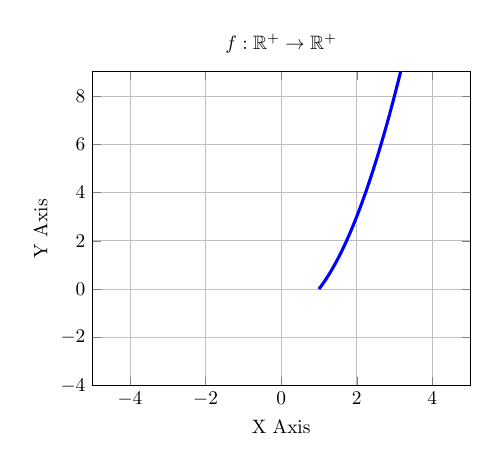
\begin{tikzpicture}[scale=0.7]
            \begin{axis}[
                xmax=5,
                xmin=-5,
                ymax=9,
                ymin=-4,
                samples=50,
                grid=major,
                xlabel={X Axis},
                ylabel={Y Axis},
                title={$f:\mathbb{R}^+\rightarrow\mathbb{R}^+$}
            ]
            \addplot[blue,ultra thick,domain=1:5](x,x^2-1);
        \end{axis}
        \end{tikzpicture}
        \label{sketch:exm-1}
    \end{subfigure}
    \hfill
    \begin{subfigure}[ht]{0.47\textwidth}
        \centering
        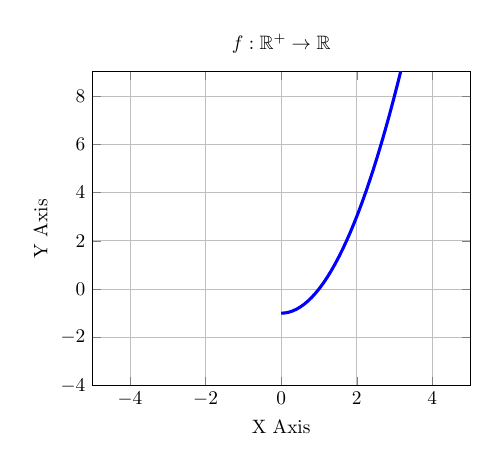
\begin{tikzpicture}[scale=0.7]
            \begin{axis}[
                xmax=5,
                xmin=-5,
                ymax=9,
                ymin=-4,
                samples=50,
                grid=major,
                xlabel={X Axis},
                ylabel={Y Axis},
                title={$f:\mathbb{R}^+\rightarrow\mathbb{R}$}
            ]
            \addplot[blue,ultra thick,domain=0:5](x,x^2-1);
        \end{axis}
        \end{tikzpicture}
        \label{sketch:exm-2}
    \end{subfigure}
    \vfill
    \begin{subfigure}[ht]{0.47\textwidth}
        \centering
        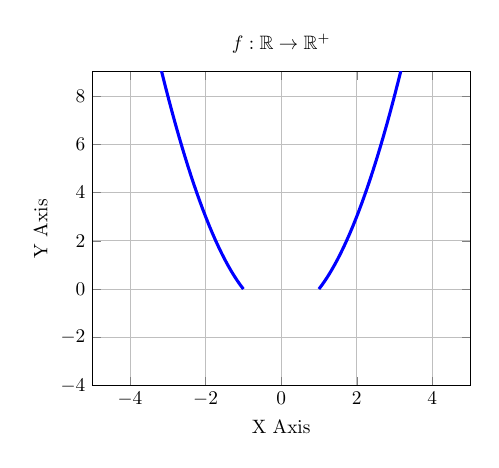
\begin{tikzpicture}[scale=0.7]
            \begin{axis}[
                xmax=5,
                xmin=-5,
                ymax=9,
                ymin=-4,
                samples=50,
                grid=major,
                xlabel={X Axis},
                ylabel={Y Axis},
                title={$f:\mathbb{R}\rightarrow\mathbb{R}^+$}
            ]
            \addplot[blue,ultra thick,domain=-5:-1](x,x^2-1);
            \addplot[blue,ultra thick,domain=1:5](x,x^2-1);
        \end{axis}
        \end{tikzpicture}
        \label{sketch:exm-3}
    \end{subfigure}
    \hfill
    \begin{subfigure}[ht]{0.47\textwidth}
        \centering
        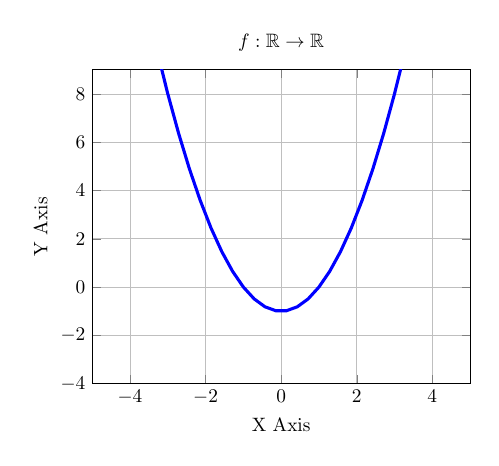
\begin{tikzpicture}[scale=0.7]
            \begin{axis}[
                xmax=5,
                xmin=-5,
                ymax=9,
                ymin=-4,
                samples=50,
                grid=major,
                xlabel={X Axis},
                ylabel={Y Axis},
                title={$f:\mathbb{R}\rightarrow\mathbb{R}$}
            ]
            \addplot[blue, ultra thick,domain=-5:9](x,x^2-1);
        \end{axis}
        \end{tikzpicture}
        \label{sketch:exm-4}
    \end{subfigure}
\end{figure}


% === End Section Includes ====

\newpage

\medskip
\printbibliography

\end{document}
